%\documentstyle[a4,twoside,epsf,makeidx]{sislman}
\documentclass[a4paper]{report}
\usepackage{sislman2}
\usepackage{graphicx}
\usepackage{fancyvrb}
\pagestyle{headings}
\usepackage{imakeidx} 
\makeindex
\begin{document}

\begin{titlepage}
  \vspace{5 cm}
  \begin{center}
  \Huge
  \textbf{SISL} \\
  \huge
  The SINTEF Spline Library \\ 
  \LARGE
  Reference Manual \\
  (version 4.5)\\ 
  \vspace{10 mm}
  \large
  SINTEF Digital, Mathematics and Cybernetics \\
  January 18, 2021
  \end{center}

\end{titlepage}

\pagenumbering{roman}
\tableofcontents
\cleardoublepage
\pagenumbering{arabic}
\setcounter{page}{1}
\chapter{Preface}
Welcome to the SISL 4.5 user's manual.  SISL stands for
\emph{\textbf{Si}ntef \textbf{S}pline \textbf{L}ibrary}, and has been gradually 
developed and enhanced for more than three decades by the geometry group at SINTEF in Oslo.
Although it is very comprehensive, its organisation is simple.  There are but a 
few structures, and its nearly four hundred main functions can usually be employed
directly and individually. This manual organises and explains the main routines.  However, much of this
information can also be found directly in the code in the form of commentaries.

The complete software package you have in your hands should contain the following:
\begin{itemize}
\item The SISL 4.5 distribution and reference guide (the document you are reading now)
\item Supplementary routines for writing SISL objects to streams (including file 
streams) in a simple ASCII format called \textbf{\Verb/Go/}.
\item A selection of \emph{sample programs}, designed to demonstrate functionalities
and use of SISL.
\item Source code for a simple \emph{viewer} that can be used to view geometric objects stored
in the \Verb/Go/-format.  This allows visual inspection of SISL-generated curves
and surfaces, as well as points.
\end{itemize}

\section{The structure of this document}
\textbf{Chapter 2} is a general introduction to SISL and its programming style. A simple example program
including instructions in how to compile and link the program and the expected output is provided.
Since it is strongly recommended that the user has some general knowledge of splines, this 
chapter also contains a couple of sections introducing the subject of spline curves and
surfaces. \\
\\
\textbf{Chapter 3 to 11} presents the main SISL routines.  \\
\\
\textbf{Chapter 12} goes through the provided sample programs and explain what these do,
and what the user can expect to learn from them.  There are a total of 15 sample 
programs, ranging from very basic to intermediate complexity.\\
\\
The goal of \textbf{Chapter 13} is to explain the use of the \emph{viewer program}, 
which is a small but handy tool for visually inspecting results from SISL routines.\\
\\
\textbf{Chapter 14} is an appendix presenting an explanation of the error codes used in SISL.\\
\\
Finally there is an \textbf{annex}, citing the text of the General Public License.

\section{The structure of the software package}\label{compile}
There are seven directories:
\begin{itemize}
\item \textbf{\Verb-include/-} - the inlude files related to the 4.5 release of SISL.
\item \textbf{\Verb-src/-} - the source code of the 4.5 release of SISL.
\item \textbf{\Verb-doc/-} - the basis for this document. 
\item \textbf{\Verb-streaming/-} - source code for the routines that can read and write
SISL objects to a stream.
\item \textbf{\Verb-examples/-} - sample programs making use of the SISL 4.5 source code.
\item \textbf{\Verb-viewer/-} - source code for a viewer that can be used to view SISL 
  objects saved in the \verb/Go/-format.
\item \textbf{\Verb-app/-} - the expected directory for test programs and applications. A
  couple of applications are provided including the example program described in Chapter 2.
\end{itemize}
Furthermore is the file CMakeLists.txt provided to facilitate building the library.

\section{Licensing information}
SISL is distibuted under the \emph{GNU Affero General Public License} (aGPL).  The license text 
is given in its entirety as an annex to this document.  Commercial licenses are also
available from SINTEF.  You can contact Tor Dokken (tor.dokken@sintef.no) for more
information.

%% *what is included in this distibution
%% *explain chapters
%% *the manual
%% *licensing information
%% *compilation
%% *the object viewer

\chapter{General Introduction}
\label{introduction}
SISL is a geometric toolkit to model with curves and surfaces. It is a
library of C functions to perform operations such as the definition,
intersection and evaluation of NURBS (Non-Uniform Rational B-spline)
geometries. Since many applications use implicit geometric
representation such as planes, cylinders, tori etc., SISL can also
handle the interaction between such geometries and NURBS.

\medskip
Throughout this manual, a distinction is made between NURBS (the
default) and B-splines. The term B-splines is used for non-uniform
non-rational (or polynomial) B-splines. B-splines are used only where it
does not make sense to employ NURBS (such as the approximation of a
circle by a B-spline) or in cases where the research
community has yet to develop stable technology for treating NURBS.
A NURBS require more memory space than a B-spline, even when the
extra degrees of freedom in a NURBS are not used. Therefore the routines
are specified to give B-spline output whenever the extra degrees of
freedom are not required.

Transferring a B-spline into NURBS format is done by constructing a new
coefficient vector using the original B-spline coefficients and setting
all the rational weights equal to one (1).
This new coefficient vector is then given as input to the routine for
creating a new curve/surface object while specifying that the object to
be created should be of the NURBS (rational B-spline) type.

To approximate a NURBS by a B-spline, use the offset calculation
routines with an offset of zero.

The routines in SISL are designed to function on curves and surfaces
which are at least continuously differentiable. However many routines
will also handle continuous curves and surfaces, including piecewise
linear ones.

\medskip
All arrays in SISL are 1-dimensional. In an array with points or vertices
are the points stored consecutively. In a raster are points or vertices
stored consecutively while points in the first parameter direction have
the shortest stride (stored right after each other). There is a special
rule for vertices given as input to a rational curve or surface, see the
Sections~\ref{sec:newCurve} and~\ref{sec:newSurf}.

The three important data structures used by SISL are SISLCurve,
SISLSurf, and SISLIntcurve. These are defined in the Curve Utilities,
Surface Utilities, and Surface Interrogation modules respectively. Other
structures are SISLBox and SISLCone, which represents a bounding box and
a normal cone, respectively. It is
important to remember to always free these structures and also to free
internally allocated structures and arrays used to pass results to the application,
otherwise strange errors might result.

In the construction of NURBS curves and surfaces is information on the order of the curve or
surface frequently required. The order is equal to the polynomial degree plus one.

The various functions are equipped with a status variable, typically
placed as the last entity in the parameter list. It returns information
about whether or not the function succeeded in its purpose. A negative
value means failure, the result zero means success while a positive
number is a warning. Section~\ref{errorcodes} provides a list over
possible error messages where most occurances are explained. 

\medskip
SISL is divided into seven modules, partly in order to provide a logical
structure, but also to enable users with a specific application to use
subsets of SISL. There are three modules dealing with curves, three with
surfaces, and one module to perform data reduction on curves and
surfaces. The modules for
curves and surfaces focus on functions for creation and definition,
intersection and interrogation, and general utilities.

The chapters 3 to 11 in this manual contain information concerning the top
level functions of each module. Lower level functions not usually
required by an application are not included. Each top level function is
documented by describing the purpose, the input and output arguments and
an example of use. Input parameters specified in the examples are suggestions, the
actual values must be set dependent on context. The geometric tolerance tells when
two points are regarded as equal. This implies that a large tolerance leads to
higher data size in approximaation type functionality such as s1360, offset curve.
In surface-surface intersections, on the other hand, will a large tolerance imply
that there is a large area around an intersection curve where the two surfaces are
closer than the tolerance, which may lead to unstability in tangential situations.
In the examples is the suggested tolerance stricter for intersection functionality
than in other cases. However, the intersection tolerance must reflect the accuracy
in which the associated geometry entities are constructed.
To get you started, this chapter contains an Example Program.

%\vfill
%\newpage

\section{\label{syntax}C Syntax Used in Manual}
This manual uses the K\&R style C syntax for historic reasons, but both
the ISO/ANSI and the K\&R C standards are supported by the library and
the include files.

\section{\label{dynamic}Dynamic Allocation in SISL}
In the description of all the functions in this manual, a
convention exists on when to declare or allocate arrays/objects outside a
function and when an array is allocated internally.
{\em NB! When memory for output arrays/objects are allocated inside a function you
must remember to free the allocated memory when it is not in use any
more.}

The convention is the following:
\begin{itemize}
\item If $[\,]$ is used in the synopsis and in the example it means
that the array has to be declared or allocated outside the function.
\item If $*$ is used it means that the function requires a
pointer and that the allocation will be done outside the function if necessary.
\item When either an array or an array of pointers or an object is to be
allocated in a function, two or three stars are used in the
synopsis.
To use the function you declare the parameter with one star less and use  \&
in the argument list.
\item For all output variables except arrays or objects
that are declared or allocated  outside the function you have to use \&
in the argument list.
\end{itemize}


\vfill
\newpage
\vfill
\newpage
\section{Creating the library}

In order to access SISL from your program you need one library inclusion, namely
the header file sisl.h. The statement
\begin{verbatim}
#include "sisl.h"
\end{verbatim}
must be written at the top of your main program.
In this header file all types
are defined.
It also contains all the
SISL top level function declarations.
Memory management and input/output require two more includes to avoid compiler warnings,
see Section~\ref{sec:exampleprog}.

SISL is prepared for makefile generation with CMake and equipped with a CMakeLists.txt file.
For information on using CMake, see www.cmake.org. The building procedure depends on whether your platform is
Linux or Windows.

\medskip
    {\noindent \bf LINUX}

Start by creating a build directory:
\begin{verbatim}
$ cd <path_to_source_code>
$ mkdir build
$ cd build
\end{verbatim}

Run the cmake program to setup the build process, selecting Debug or Release
as build type, optionally selecting a local install folder:
\begin{verbatim}
$ cmake .. -DCMAKE_BUILD_TYPE=Release (-DCMAKE_INSTALL_PREFIX=$HOME/install)
\end{verbatim}

For a gui-like cmake interface use ccmake (from cmake-ncurses-gui) or cmake-gui (from cmake.org).

Build the library:
\begin{verbatim}
$ make
\end{verbatim}
This will install the library in the build folder. Compilation and build of one particular
example program is done by a specific make statement:
\begin{verbatim}
$ make example01
\end{verbatim}
This option requires compilation of examples to be set in the Makefile.

Install the library to a local folder (requires the use of
-DCMAKE\_INSTALL\_PREFIX with a local folder in the previous step):
\begin{verbatim}
$ make install
\end{verbatim}

If the -DCMAKE\_INSTALL\_PREFIX in the cmake step was omitted or was set to a
system folder (like /usr/local) the user needs elevated privileges to install
the library:
\begin{verbatim}
$ sudo make install
\end{verbatim}

\medskip
{\noindent \bf Windows}

Add a new build folder somewhere. Start the CMake
executable and fill in the paths to the source and build folders. When
you run CMake, a Visual Studio project solution file will be generated
in the build folder.



\newpage
\section{An Example Program} \label{sec:exampleprog}

To clarify the previous section here is an example program designed to
test the SISL algorithm for intersecting a cone with
a B-spline curve. The program calls the SISL routines newCurve() documented in
Section ~\ref{sec:newCurve}, freeCurve() documented in~\ref{sec:freeCurve},
s1373() found in Section~\ref{sec:s1373} and freeIntcrvlist() in~\ref{sec:freeIntcrvlist}.

\begin{verbatim}
#include "sisl.h"
#include <stdlib.h>  
#include <stdio.h>

int main()
{
  SISLCurve *pc=0;                    /* Pointer to spline curve */
  double aepsco,aepsge;               /* Tolerances */
  double top[3],axispt[3],conept[3];  /* Representating the cone */
  double st[100],scoef[100];          /* Knot vector and coefficients of spline curve */
  double *spar;                       /* Parameter values of intersection points */
  int kstat;                          /* Return status from function calls */
  int cone_exists=0;
  int kk,kn,kdim;                     /* Order (polynomial degree+1), number of 
                                         coefficients and spatial dimension */
  int ki;                             /* Counter */
  int kpt,kcrv;                       /* Number of intersection points and curves */
  SISLIntcurve **qrcrv;               /* Array of pointer to intersection curves  */
  char ksvar[100];                    
  kdim=3;
  aepsge=0.001; /* Geometric tolerance */
  aepsco=0.000001; /* Computational tolerance. This parameter is included from 
                      historical reasons and no longer used */

  ksvar[0] = '0';  /* Arbitrary character */
  while (ksvar[0] != 'q')
    {
      printf("\n cu - define a new B-spline curve");
      printf("\n co - define a new cone");
      printf("\n i - intersect the B-spline curve with the cone");
      printf("\n q - quit");
      printf("\n> ");
      scanf("%s",ksvar);

      if (ksvar[0] == 'c' && ksvar[1] == 'u')
        {
          /* Define spline curve */
          printf("\n Give number of vertices, order of curve: ");
          scanf("%d %d", &kn, &kk);
          printf("Give knots values in ascending order: \n");
          for (ki=0; ki<kn+kk; ki++)
            {
               scanf("%lf",&st[ki]);
            }
          printf("Give vertices \n");
          for (ki=0; ki<kn*kdim; ki++)
            {
              scanf("%lf",&scoef[ki]);
            }
         if(pc) freeCurve(pc);

          /* Create curve */
          pc = newCurve(kn,kk,st,scoef,1,kdim,1);
        }
      else if (ksvar[0] == 'c' && ksvar[1] == 'o')
       {
         printf("\n Give top point: ");
         scanf("%lf %lf %lf",&top[0],&top[1],&top[2]);
         printf("\n Give a point on the axis: ");
         scanf("%lf %lf %lf",&axispt[0],&axispt[1],&axispt[2]);
         printf("\n Give a point on the cone surface: ");
         scanf("%lf %lf %lf",&conept[0],&conept[1],&conept[2]);
         cone_exists=1;
       }
      else if (ksvar[0] == 'i' && cone_exists && pc)
       {
         /* Intersect spline curve with cone */
         s1373(pc,top,axispt,conept,kdim,aepsco,aepsge,
               &kpt,&spar,&kcrv,&qrcrv,&kstat);
         printf("\n kstat %d",kstat);
         printf("\n kpt %d",kpt);
         printf("\n kcrv %d",kcrv);
         for (ki=0;ki<kpt;ki++)
          {
            printf("\nIntersection point %lf",spar[ki]);
          }
        if (spar)
          {
            /* The array containing parameter values of the intersection points between
               the curve and the cone is allocated inside s1373 and must be freed */
            free (spar);
            spar=0;
          }
        if (qrcrv)
         {
           /* The array containing pointers to intersection points curves between
              the curve and the cone is allocated inside s1373 and must be freed.
              This is done in a special function taking care of the intersection
              curves themselves */
          freeIntcrvlist(qrcrv,kcrv);
          qrcrv=0;
        }
      }
    }
  return 0;
}

\end{verbatim}
Note that sisl.h is included. stdlib.h is included to declare free, which
releases memory allocated in the function s1373. stdio.h declares printf and
scanf.

\bigskip

The program was compiled and built using the command:
\begin{verbatim}
$ make prog1
\end{verbatim}
Note that the program must be placed in the app folder and sisl\_COMPILE\_APPS must be set to true.

A sample run of prog1 went as follows:
\begin{verbatim}
$ prog1

     cu - define a new B-spline curve
     co - define a new cone
     i  - intersect the B-spline curve with the cone
     q  - quit
> cu

 Give number of vertices, order of curve: 2 2
Give knots values in ascending order:
0 0 1 1
Give vertices
1 0 0.5
-1 0 0.5

     cu - define a new B-spline curve
     co - define a new cone
     i  - intersect the B-spline curve with the cone
     q  - quit
> co

 Give top point: 0 0 1

 Give a point on the axis: 0 0 0

 Give a point on the cone surface: 1 0 0

     cu - define a new B-spline curve
     co - define a new cone
     i  - intersect the B-spline curve with the cone
     q  - quit
> i

 kstat 0
 kpt   2
 kcrv  0
Intersection point 0.250000
Intersection point 0.750000
     cu - define a new B-spline curve
     co - define a new cone
     i  - intersect the B-spline curve with the cone
     q  - quit
> q
$
\end{verbatim}
SISL found two intersection points given by the parameters
$0.25$ and $0.75$. These parameters correspond to the 3D points
$(-0.5,0,0.5)$ and $(0.5,0,0.5)$ (which could be found by calling
the evaluation routine s1221()). They lie on both
the B-spline curve and the cone --- as expected!

\section{B-spline Curves}

This section is optional reading for those who want to
become acquainted with some of the mathematics of
B-splines curves. For a description of the data structure for
B-spline curves in SISL, see the SISL 4.4 manual.

A B-spline curve is defined by the formula
$$ {\bf c}(t) = \sum_{i=1}^{n} {\bf p}_{i} B_{i,k,{\bf t}}(t). $$
The dimension of the curve ${\bf c}$ is equal to that of its
{\it control points} ${\bf p}_i$. For example, if the dimension of the
control points
is one, the curve is a function, if the dimension is two,
the curve is planar, and if the dimension is three,
the curve is spatial.
Usually the dimension of the curve will be at most three,
but SISL also allows higher dimensions.

Thus, a B-spline curve is a linear combination of a sequence of B-splines
$B_{i,k,{\bf t}}$ (called a B-basis)
uniquely determined by a knot vector ${\bf t}$ and
the order $k$. Order is equivalent to polynomial degree plus one.
For example, if the order is two, the degree is one and the B-splines
and the curve $c$ they generate are (piecewise) linear.
If the order is three, the degree is two and the B-splines and
the curve are quadratic. Cubic B-splines and
curves have order 4 and degree 3, etc.

The parameter range of a B-spline curve ${\bf c}$ is the interval
$$ [t_k, t_{n+1}], $$
and so mathematically, the curve is a mapping
${\bf c}: [t_k, t_{n+1}] \to \RR^d$, where $d$ is the Euclidean space
dimension of its control points.

The complete representation of a B-spline curve consists of
\begin{description}
\item[$dim$]: The dimension of the underlying Euclidean space,
              $1,2,3,\ldots$.
\item[$n$]: The number of vertices (also the number of B-splines)
\item[$k$]: The order of the B-splines.
\item[${\bf t}$]: The knot vector of the B-splines.
            ${\bf t} = (t_1, t_2, \ldots, t_{n+k})$.
\item[${\bf p}$]: The control points of the B-spline curve.
           $p_{d,i}\;,\; d=1,\ldots,dim\;,\;
                i=1,\ldots,n.\;\;$
                e.g. when $dim = 3$, we have
                ${\bf p} = (x_1,y_1,z_1,x_2,y_2,z_2,\ldots,x_n,y_n,z_n)$.
\end{description}

We note that arrays in $c$ start at index 0 which means,
for example, that if the array $t$ holds the knot vector,
then $t[0] = t_1,\ldots, t[n+k-1] = t_{n+k}$
and the parameter interval goes from
$t[k-1]$ to $t[n]$. Similar considerations apply to the other arrays.

The data in the representation must satisfy certain conditions:
\begin{itemize}
\item The knot vector must be non-decreasing: $t_i \le t_{i+1}$.
      Moreover, two knots $t_i$ and $t_{i+k}$ must be distinct:
      $t_i < t_{i+k}$.
\item The number of vertices should be greater than or equal
      to the order of the curve: $n \ge k$.
\item There should be $k$ equal knots at the beginning and at the end
      of the knot vector; that is the knot vector ${\bf t}$
      must satisfy the conditions $t_1 = t_2 = \ldots = t_k$
      and $t_{n+1} = t_{n+2} = \ldots = t_{n + k}$.
\end{itemize}

To understand the representation better, we will look at
three parts of the
representation: the B-splines (the basis functions),
the knot vector and the control polygon.

\subsection{B-splines}

A set of B-splines is determined by the order $k$
and the knots. For example,
to define a single B-spline of degree one, we need three knots.
In figure~\ref{curve1} the three knots are marked as dots.
Knots can also be equal as shown in figure
\ref{curve2}.
By taking a linear combination of the three types of B-splines shown
in figures~\ref{curve1} and~\ref{curve2}
we can generate a linear spline function
as shown in figure~\ref{curve3}.
\begin{figure}
        \begin{center}
                \begin{picture}(250,80)(0,0)
                \put(80,0){\circle*{2}}
                \put(150,0){\circle*{2}}
                \put(230,0){\circle*{2}}

                \put(30,4){\vector(0,1){76}}
                \put(28,10){\line(1,0){4}}
                \put(28,70){\line(1,0){4}}
                \put(20,10){\makebox(0,0){0.0}}
                \put(20,70){\makebox(0,0){1.0}}

                \thicklines
                \put(80,10){\line(6,5){70}}
                \put(150,70){\line(4,-3){80}}
                \end{picture}\\
        \end{center}
  \caption{\label{curve1}A linear B-spline (order 2) defined by
                        three knots.}
\end{figure}
\begin{figure}
        \begin{center}
                \begin{picture}(300,85)(0,0)
                \put(40,0){\circle*{2}}
                \put(280,0){\circle*{2}}
                \put(120,5){\circle*{2}}
                \put(200,5){\circle*{2}}
                \put(40,5){\circle*{2}}
                \put(280,5){\circle*{2}}

                \put(20,9){\vector(0,1){76}}
                \put(18,15){\line(1,0){4}}
                \put(18,75){\line(1,0){4}}
                \put(10,15){\makebox(0,0){0.0}}
                \put(10,75){\makebox(0,0){1.0}}

                \put(170,9){\vector(0,1){76}}
                \put(168,15){\line(1,0){4}}
                \put(168,75){\line(1,0){4}}
                \put(160,15){\makebox(0,0){0.0}}
                \put(160,75){\makebox(0,0){1.0}}

                \thicklines
                \put(120,15){\line(-4,3){80}}
                \put(200,15){\line(4,3){80}}
                \end{picture}\\
        \end{center}
  \caption{\label{curve2}Linear B-splines of with multiple knots at one end.}
\end{figure}
\begin{figure}
        \begin{center}
                \begin{picture}(300,90)(0,0)
                \put(0,0){\circle*{2}}
                \put(0,5){\circle*{2}}
                \put(60,5){\circle*{2}}
                \put(120,5){\circle*{2}}
                \put(160,5){\circle*{2}}
                \put(240,5){\circle*{2}}
                \put(300,5){\circle*{2}}
                \put(300,0){\circle*{2}}

                \multiput(0,10)(12,10){5}{\line(6,5){10}}
                \multiput(60,10)(-12,8){5}{\line(-3,2){10}}
                \multiput(60,10)(12,2){5}{\line(6,1){10}}
                \multiput(120,10)(-12,10){5}{\line(-6,5){10}}
                \multiput(120,10)(12,6){3}{\line(2,1){10}}
                \multiput(160,10)(-12,3){3}{\line(-4,1){10}}
                \multiput(160,10)(12,12){6}{\line(1,1){10}}
                \multiput(240,10)(-12,3){6}{\line(-4,1){10}}
                \multiput(240,10)(12,12){5}{\line(1,1){10}}
                \multiput(300,10)(-12,16){5}{\line(-3,4){10}}

                \thicklines
                \put(0,50){\line(6,1){60}}
                \put(60,60){\line(3,-2){60}}
                \put(120,20){\line(4,1){40}}
                \put(160,30){\line(4,3){80}}
                \put(240,90){\line(3,-1){60}}
                \end{picture}\\
        \end{center}
  \caption{\label{curve3}A B-spline curve of dimension 1 as a linear
            combination of a sequence of B-splines.
            Each B-spline (dashed) is scaled by a coefficient.}
\end{figure}

A quadratic B-spline is a linear combination of two linear
B-splines. Shown in figure~\ref{curve4}
is a quadratic B-spline defined by four knots.
A quadratic B-spline is
the sum of two products, the first product between the linear B-spline
on the left and a corresponding line from 0 to 1,
the second product between the linear B-spline
on the right and a corresponding line from 1 to 0;
see figure~\ref{curve4}.
For higher degree B-splines there is a similar definition.
A B-spline of order $k$ is the sum of two B-splines of
order $k-1$, each weighted with weights in the interval [0,1].
In fact we define B-splines of order 1 explicitly as box functions,
$$  B_{i,1}(t) =  \cases{1 & if $t_i \le t < t_{i+1}$; \cr
                              0 &  otherwise, \cr } $$
and then the complete definition of a $k$-th order B-spline is
$$ B_{i,k}(t) = {t - t_i \over t_{i+k-1} - t_i} B_{i,k-1}(t)
             +
             {t_{i+k} - t \over t_{i+k} - t_{i+1}} B_{i-1,k-1}(t). $$

\begin{figure}
        \begin{center}
                \begin{picture}(250,70)(0,0)

                \put(10,4){\vector(0,1){76}}
                \put(8,10){\line(1,0){4}}
                \put(8,70){\line(1,0){4}}
                \put(0,10){\makebox(0,0){0.0}}
                \put(0,70){\makebox(0,0){1.0}}

                \put(35,0){\circle*{2}}
                \put(95,0){\circle*{2}}
                \put(155,0){\circle*{2}}
                \put(215,0){\circle*{2}}

                \multiput(35,10)(18,9){7}{\line(2,1){10}}
                \multiput(215,10)(-18,9){7}{\line(-2,1){10}}

                \thicklines
                \put(35,10){\line(1,1){60}}
                \put(95,10){\line(1,1){60}}
                \put(155,10){\line(-1,1){60}}
                \put(215,10){\line(-1,1){60}}

                \bezier{70}(35,10)(65,10)(95,40)
                \bezier{70}(95,40)(125,70)(155,40)
                \bezier{70}(215,10)(185,10)(155,40)
                \end{picture}\\
        \end{center}
  \caption{\label{curve4}A quadratic B-spline, the two linear
           B-splines and the corresponding lines (dashed)
           in the quadratic B-spline definition.}
\end{figure}

B-splines satisfy some important properties for curve and surface design.
Each B-spline is non-negative and it can be shown that they sum to
one,
$$ \sum_{i=1}^{n}B_{i,k,{\bf t}}(t) = 1. $$
These properties combined mean that B-spline curves
satisfy the {\it convex hull property}: the curve lies in the convex
hull of its control points.
Furthermore, the support of the B-spline $B_{i,k,{\bf t}}$ is
the interval $[t_i,t_{i+k}]$ which means that B-spline
curves has {\it local control}: moving one control point only
alters the curve locally.

Due to the demand of $k$ multiple knots at the ends of the knot
vector, B-spline curves in SISL also have the {\it endpoint property}:
the start point of the B-spline curve
equals the first control point and the end point equals the
last control point, in other words
$$ {\bf c}(t_k) = {\bf p}_1
     \qquad \hbox{and} \qquad
   {\bf c}(t_{n+1}) = {\bf p}_n. $$

\subsection{\label{contrlpoly}The Control Polygon}

The control points ${\bf p}_i$ define the vertices
The {\it control polygon} of a B-spline curve is the polygonal
arc formed by its control points,
${\bf p}_0, {\bf p}_1, \ldots,{\bf p}_n$.
This means that
the control polygon, regarded as a parametric curve,
is itself piecewise linear B-spline curve (order two).
If we increase the order, the distance between the control polygon
and the curve increases (see figure~\ref{curve5}).
A higher order B-spline curve tends to smooth
the control polygon and at the same time mimic its shape.
For example, if the control polygon is convex, so is the B-spline curve.

Another property of the control polygon is that it will get closer
to the curve if it is redefined by inserting knots into the curve
and thereby increasing the number of vertices;
see figure~\ref{curve6}.
If the refinement is infinite then the control polygon converges to the curve.
\begin{figure}
        \begin{center}
                \begin{picture}(240,80)(0,0)
                \thicklines
                \put(0,40){\line(2,1){80}}
                \put(80,80){\line(1,-1){80}}
                \put(160,0){\line(1,1){80}}

                \bezier{120}(0,40)(80,80)(120,40)
                \bezier{120}(120,40)(160,0)(240,80)

                \bezier{120}(0,40)(60,70)(120,40)
                \bezier{120}(120,40)(180,20)(240,80)

                \end{picture}\\
        \end{center}
  \caption{\label{curve5}Linear, quadratic, and cubic B-spline
           curves sharing the same control polygon. The control polygon is
                equal to the linear B-spline curve. The curves
                are planar, i.e. the space dimension is two.}
\end{figure}

\begin{figure}
        \begin{center}
                \begin{picture}(240,80)(0,0)
                \thicklines
                \put(0,40){\line(2,1){40}}
                \put(40,60){\line(5,0){40}}
                \put(80,60){\line(2,-1){60}}
                \put(140,30){\line(6,1){60}}
                \put(200,40){\line(1,1){40}}

                \bezier{120}(0,40)(60,70)(120,40)
                \bezier{120}(120,40)(180,20)(240,80)

                \end{picture}\\
        \end{center}
  \caption{\label{curve6}The cubic B-spline curve with a
                redefined knot vector.}
\end{figure}

\subsection{The Knot Vector}

The knots of a B-spline curve describe the following properties of the curve:
\begin{itemize}
\item The parameterization of the B-spline curve
\item The continuity at the joins between the adjacent polynomial
   segments of the B-spline curve.
\end{itemize}
In figure~\ref{curve7} we have two curves
with the same control polygon and order but
with different parameterization.

This example is not meant as an encouragement to use
parameterization for modelling, rather to make users
aware of the effect of parameterization. Something close to
curve length parameterization is in most cases
preferable. For interpolation, chord-length parameterization
is used in most cases.

The number of equal knots determines the degree
of continuity. If $k$ consecutive internal knots are equal,
the curve is discontinuous.
Similarly if $k-1$ consecutive internal knots are equal,
the curve is continuous but not in general differentiable.
A continuously differentiable curve
with a discontinuity in the second derivative
can be modelled using $k-2$ equal knots etc. (see figure~\ref{curve8}).
Normally, B-spline curves in SISL are expected to be continuous.
For intersection algorithms, curves are usually expected to
be continuously differentiable ($C^1$).

\begin{figure}
        \begin{center}
                \begin{picture}(240,240)(0,0)
                \thicklines
                \put(0,130){\circle*{2}}
                \put(0,135){\circle*{2}}
                \put(0,140){\circle*{2}}
                \put(240,130){\circle*{2}}
                \put(240,135){\circle*{2}}
                \put(240,140){\circle*{2}}

                \put(60,140){\circle*{2}}
                \put(180,10){\circle*{2}}


                \put(0,0){\circle*{2}}
                \put(0,5){\circle*{2}}
                \put(0,10){\circle*{2}}
                \put(240,0){\circle*{2}}
                \put(240,5){\circle*{2}}
                \put(240,10){\circle*{2}}

                \put(0,185){\line(2,1){80}}
                \put(80,225){\line(1,-1){80}}
                \put(160,145){\line(1,1){80}}

                \put(0,55){\line(2,1){80}}
                \put(80,95){\line(1,-1){80}}
                \put(160,15){\line(1,1){80}}

                \bezier{130}(0,185)(80,225)(100,205)
                \bezier{160}(100,205)(160,145)(240,225)

                \bezier{160}(0,55)(80,95)(140,35)
                \bezier{130}(140,35)(160,15)(240,95)
                \end{picture}\\
        \end{center}
  \caption{\label{curve7}Two quadratic B-spline curves with the same
control polygon but different knot vectors. The curves and the control
polygons are two-dimensional.}
\end{figure}

\begin{figure}
        \begin{center}
                \begin{picture}(300,90)(0,0)
                \thicklines
                \put(0,0){\circle*{2}}
                \put(0,5){\circle*{2}}
                \put(0,10){\circle*{2}}

                \put(150,5){\circle*{2}}
                \put(150,10){\circle*{2}}

                \put(300,0){\circle*{2}}
                \put(300,5){\circle*{2}}
                \put(300,10){\circle*{2}}

                \bezier{200}(0,50)(80,90)(150,20)
                \bezier{200}(150,20)(220,80)(300,90)
                \end{picture}\\
        \end{center}
  \caption{\label{curve8}A quadratic B-spline curve with two
equal internal knots.}
\end{figure}

\subsection{NURBS Curves}

A NURBS (Non-Uniform Rational B-Spline) curve is a generalization
of a B-spline curve,
$$ {\bf c}(t) = {\sum_{i=1}^{n} w_i {\bf p}_{i} B_{i,k,{\bf t}}(t)
                 \over
                 \sum_{i=1}^{n} w_i B_{i,k,{\bf t}}(t)} . $$
In addition to the data of a B-spline curve, the NURBS curve
${\bf c}$ has a sequence of weights $w_1,\ldots,w_n$.
One of the advantages of NURBS curves over B-spline curves is that
they can be used to represent conic sections exactly (taking the
order $k$ to be three).
A disadvantage is that NURBS curves depend nonlinearly on their weights,
making some calculations, like the evaluation of derivatives,
more complicated and less efficient than with B-spline curves.

The representation of a NURBS curve is the same as for a B-spline
except that it also includes
\begin{description}
\item[${\bf w}$]: A sequence of weights
            ${\bf w} = (w_1, w_2, \ldots, w_n)$.
\end{description}

In SISL we make the assumption that
\begin{itemize}
\item The weights are (strictly) positive: $w_i > 0$.
\end{itemize}

Under this condition, a NURBS curve, like its B-spline cousin,
enjoys the convex hull property. 
Due to $k$-fold knots at the ends of the knot vector,
NURBS curves in SISL also have the endpoint property.


\section{B-spline Surfaces}

This section is optional reading for those who want to
become acquainted with some of the mathematics of
tensor-product B-splines surfaces. For a description of the data structure for
B-spline surfaces in SISL, see the reference manual.

A tensor product B-spline surface is defined as
\[{\bf s}(u,v) = \sum_{i=1}^{n_1}\sum_{j=1}^{n_2}{\bf p}_{i,j} 
	B_{i,k_1,{\bf u}}(u) B_{j,k_2,{\bf v}}(v) \]
with control points ${\bf p}_{i,j}$ and two variables
(or parameters) $u$ and $v$.
The formula shows that a basis function of a B-spline surface is a
product of two basis functions of B-spline curves (B-splines).
This is why a B-spline surface is called a tensor-product surface.
The following is a list of the components of the representation:
\begin{description}
\item[$dim$]: The dimension of the underlying Euclidean space.
\item[$n_1$]: The number of vertices with respect to the first parameter.
\item[$n_1$]: The number of vertices with respect to the second parameter.
\item[$k_1$]: The order of the B-splines in the first parameter.
\item[$k_2$]: The order of the B-splines in the second parameter.
\item[${\bf u}$]: The knot vector of the B-splines with respect to
                  the first parameter,
                  ${\bf u} = (u_1,u_2,\ldots,u_{n_1+k_1})$.
\item[${\bf v}$]: The knot vector of the B-splines with respect to
                  the second parameter,
                  ${\bf v} = (v_1,v_2,\ldots,v_{n_2+k_2})$.
\item[${\bf p}$]: The control points of the B-spline surface,
           $c_{d,i,j}$, $d=1,\ldots,dim$, $i=1,\ldots,n_1$,
		$j=1,\ldots,n_2$.
	When $dim = 3$, we have
          ${\bf p} = (x_{1,1},y_{1,1},z_{1,1},x_{2,1},y_{2,1},z_{2,1},\ldots$,
                  $x_{n_1,1},y_{n_1,1},z_{n_1,1},\ldots$,
                     $x_{n_1,n_2},y_{n_1,n_2},z_{n_1,n_2})$.
\end{description}

The data of the B-spline surface must fulfill the following requirements:
\begin{itemize}
\item
Both knot vectors must be non-decreasing.
\item
The number of vertices must be greater than or equal to the order
with respect to both parameters: $n_1 \ge k_1$ and $n_2 \ge k_2$.
\item
There should be $k_1$ equal knots at the beginning and end 
of knot vector ${\bf u}$ and $k_2$ equal knots at the beginning and
end of knot vector ${\bf v}$.
\end{itemize}

The properties of the representation of a B-spline surface are
similar to the properties of the representation of a B-spline curve.
The control points ${\bf p}_{i,j}$ form a {\it control net} as shown in
figure~\ref{surf1}.
The control net has similar properties to the control
polygon of a B-spline curve, described in section~\ref{contrlpoly}.
A B-spline surface has two knot vectors, one
for each parameter. In figure~\ref{surf1} we can
see {\it isocurves}, surface curves
defined by fixing the value of one of the parameters.

\begin{figure}
\vspace{50 mm}
  \special{psfile=surf1.ps hoffset=-30 voffset=-170 hscale=90 vscale=60}
  %\special{psfile=surf1.ps hoffset=95 hscale=40 vscale=40}
%  \epsffile{surf1.ps}
  \caption{\label{surf1}
		A B-spline surface and its control net.
		The surface is drawn using isocurves.
		The dimension is 3.}
\end{figure}

\subsection{The Basis Functions}

A basis function of a B-spline surface is the product of two
basis functions of two B-spline curves,
\[ B_{i,k_1,{\bf u}}(u) B_{j,k_2,{\bf v}}(v). \]
Its support is the rectangle $[u_i,u_{i+k_1}] \times [v_j,v_{j+k_2}]$.
If the basis functions in both directions are of degree one and all
knots have multiplicity one, then the surface basis functions are
pyramid-shaped 
(see figure~\ref{surf2}).
For higher degrees, the surface basis functions are bell shaped.

\begin{figure}
	\begin{center}
		\begin{picture}(250,125)(0,0)

		\put(10,39){\vector(0,1){86}}
		\put(8,45){\line(1,0){4}}
		\put(8,120){\line(1,0){4}}
		\put(0,45){\makebox(0,0){0.0}}
		\put(0,120){\makebox(0,0){1.0}}

		\put(50,5){\circle*{2}}
		\put(100,5){\circle*{2}}
		\put(150,5){\circle*{2}}

		\put(190,20){\circle*{2}}
		\put(215,45){\circle*{2}}
		\put(240,70){\circle*{2}}

		\thicklines
		\put(65,20){\line(1,0){100}}
		\put(165,20){\line(1,1){50}}
		\multiput(65,20)(18,18){3}{\line(1,1){10}}
		\multiput(115,70)(20,0){5}{\line(1,0){10}}


		\put(65,20){\line(3,4){75}}
		\put(165,20){\line(-1,4){25}}
		\put(215,70){\line(-3,2){75}}
		\multiput(115,70)(8,16){3}{\line(1,2){5}}
		\end{picture}\\
	\end{center}

  \caption{\label{surf2}
		A basis function of degree one in
		both variables.}
\end{figure}

\subsection{NURBS Surfaces}

A NURBS (Non-Uniform Rational B-Spline) surface is a generalization
of a B-spline surface,
$$ {\bf s}(u,v) = {\sum_{i=1}^{n_1}\sum_{j=1}^{n_2} w_{i,j} {\bf p}_{i,j} 
	    B_{i,k_1,{\bf u}}(u) B_{j,k_2,{\bf v}}(v)  \over
             \sum_{i=1}^{n_1}\sum_{j=1}^{n_2} w_{i,j}
	         B_{i,k_1,{\bf u}}(u) B_{j,k_2,{\bf v}}(v)}. $$
In addition to the data of a B-spline surface, the NURBS surface
has a weights $w_{i,j}$.
NURBS surfaces can be used to exactly represent several common
`analytic' surfaces such as spheres, cylinders, tori, and cones.
A disadvantage is that NURBS surfaces depend nonlinearly on their weights,
making some calculations, like with NURBS curves,
less efficient.

The representation of a NURBS surface is the same as for a B-spline
except that it also includes
\begin{description}
\item[${\bf w}$]: The weights of the NURBS surface,
           $w_{i,j}$, $i=1,\ldots,n_1$, $j=1,\ldots,n_2$, so
          ${\bf w} = (w_{1,1},w_{2,1},\ldots,w_{n_1,1},\ldots$,
                  $w_{1,2},\ldots,w_{n_1,n_2})$.
\end{description}
In SISL we make the assumption that
\begin{itemize}
\item The weights are (strictly) positive: $w_{i,j} > 0$.
\end{itemize}



\vfill
\newpage
%\mbox{}
%\newpage

\cleardoublepage
\chapter{Curve Definition}
\label{curvedefinition}

This chapter describes all functions in the Curve Definition module.
\section{Interpolation}
In this section we treat different kinds of interpolation of
points or points and derivatives (Hermite). In addition to the general
functions there are functions to find fillet curves
(a curve between two other curves),
and blending curves (a curve between the end points of two other curves).
\subsection{Compute a curve interpolating a straight line between two points.}
\funclabel{s1602}
\begin{minipg1}
To make a straight line represented as a B-spline curve between two points.
\end{minipg1}\\ \\
SYNOPSIS\\
        \>void s1602(\begin{minipg3}
                {\fov startpt}, {\fov endpt}, {\fov order}, {\fov dim}, {\fov startpar}, {\fov endpar},
                {\fov curve}, {\fov stat})
                \end{minipg3}\\[0.3ex]
                \>\>    double  \>      {\fov startpt}[\,];\\
                \>\>    double  \>      {\fov endpt}[\,];\\
                \>\>    int     \>      {\fov order};\\
                \>\>    int     \>      {\fov dim};\\
                \>\>    double  \>      {\fov startpar};\\
                \>\>    double  \>      *{\fov endpar};\\
                \>\>    SISLCurve       \>      **{\fov curve};\\
                \>\>    int     \>      *{\fov stat};\\
\newpagetabs
ARGUMENTS\\
        \>Input Arguments:\\
        \>\>    {\fov startpt}  \> - \> Start point of the straight line\\
        \>\>    {\fov endpt}    \> - \> End point of the straight line\\
        \>\>    {\fov order}    \> - \> The order of the curve to be made.\\
        \>\>    {\fov dim}      \> - \> The dimension of the geometric space\\
        \>\>    {\fov startpar} \> - \> Start value of the parameterization of the curve\\
\\
        \>Output Arguments:\\
        \>\>    {\fov endpar }\> - \>   Parameter value used at the end of the curve\\
        \>\>    {\fov curve}    \> - \> Pointer to the B-spline curve\\
        \>\>    {\fov stat}     \> - \> Status messages\\
                \>\>\>\>\>              $> 0$   : warning\\
                \>\>\>\>\>              $= 0$   : ok\\
                \>\>\>\>\>              $< 0$   : error\\
\\
EXAMPLE OF USE\\
                \>      \{ \\
                \>\>    double          \>{\fov startpt}[2];\\
                \>\>    double          \>{\fov endpt}[2];\\
                \>\>    int             \>{\fov order};\\
                \>\>    int             \>{\fov dim};\\
                \>\>    double          \>{\fov startpar};\\
                \>\>    double          \>{\fov endpar};\\
                \>\>    SISLCurve               \>*{\fov curve};\\
                \>\>    int             \>{\fov stat};\\
                \>\>    \ldots \\
        \>\>s1602(\begin{minipg4}
                {\fov startpt}, {\fov endpt}, {\fov order}, {\fov dim},
        {\fov startpar}, \&{\fov endpar}, \&{\fov curve}, \&{\fov stat});
                        \end{minipg4}\\
                \>\>    \ldots \\
                \>      \} \\
\end{tabbing}

\pgsbreak
\subsection{Compute a curve interpolating a set of points,
\mbox{automatic} parameterization.}
\funclabel{s1356}
\begin{minipg1}
Compute a curve interpolating a set of points.  The points
can be assigned a tangent (derivative).  The parameterization of the
curve will be generated and the curve can be open, closed non-periodic
or periodic.  If end-conditions are conflicting, the condition closed
curve rules out other end conditions.
The output will be represented as a B-spline curve.
\end{minipg1} \\ \\
SYNOPSIS\\
        \>void s1356(\begin{minipg3}
          {\fov epoint}, {\fov inbpnt}, {\fov idim}, {\fov nptyp}, {\fov icnsta}, {\fov icnend}, {\fov iopen}, {\fov ik}, {\fov astpar},
          {\fov cendpar}, {\fov rc}, {\fov gpar}, {\fov jnbpar}, {\fov jstat})
        \end{minipg3}\\[0.3ex]
        \>\>    double \>  {\fov epoint}[\,];\\
        \>\>    int    \>  {\fov inbpnt};\\
        \>\>    int    \>  {\fov idim};\\
        \>\>    int    \>  {\fov nptyp}[\,];\\
        \>\>    int    \>  {\fov icnsta};\\
        \>\>    int    \>  {\fov icnend};\\
        \>\>    int    \>  {\fov iopen};\\
        \>\>    int    \>  {\fov ik};\\
        \>\>    double \>  {\fov astpar};\\
        \>\>    double \>  *{\fov cendpar};\\
        \>\>    SISLCurve \> **{\fov rc};\\
        \>\>    double \>  **{\fov gpar};\\
        \>\>    int    \>  *{\fov jnbpar};\\
        \>\>    int    \>  *{\fov jstat};\\
\\
ARGUMENTS\\
        \>Input Arguments:\\
        \>\>    {\fov epoint}\> - \>
        \begin{minipg2}
          Array (of length $idim\times inbpnt$) containing the
          points/\-derivatives to be interpolated.
        \end{minipg2}\\
        \>\>    {\fov inbpnt}\> - \>
        \begin{minipg2}
          No. of points/\-derivatives in the {\fov epoint} array.
        \end{minipg2}\\
        \>\>    {\fov idim}\> - \>
        The dimension of the space in which the points lie.\\
        \>\>    {\fov nptyp}\> - \> \begin{minipg2}
                  Array (length {\fov inbpnt}) containing type indicator for
                  points/\-derivatives/\-second-derivatives:
                \end{minipg2}\\
                \>\>\>\> $=1$\>: Ordinary point.\\
                \>\>\>\> $=2$\>:
                \begin{minipg5}
                  Knuckle point.  (Is treated as an ordinary point.)
                \end{minipg5}\\
                \>\>\>\> $=3$\>: Derivative to next point.\\
                \>\>\>\> $=4$\>: Derivative to prior point.\\
                \>\>\>\> ($=5$\>: Second-derivative to next point.)\\
                \>\>\>\> ($=6$\>: Second derivative to prior point.)\\
                \>\>\>\> $=13$\>: Point of tangent to next point.\\
                \>\>\>\> $=14$\>: Point of tangent to prior  point.\\
\newpagetabs
        \>\>    {\fov icnsta}\> - \>
                Additional condition at the start of the curve:\\
                  \>\>\>\> $=0$\>: No additional condition.\\
                  \>\>\>\> $=1$\>: Zero curvature at start.\\
        \>\>    {\fov icnend}\> - \>
                Additional condition at the end of the curve:\\
                  \>\>\>\> $=0$\>: No additional condition.\\
                  \>\>\>\> $=1$\>: Zero curvature at end.\\
        \>\>    {\fov iopen}\> - \>
                Flag telling if the curve should be open or closed:\\
                  \>\>\>\> $=1$\>: Open curve.\\
                  \>\>\>\> $=0$\>: Closed, non-periodic curve.\\
                  \>\>\>\> $=-1$\>: Periodic (and closed) curve.\\
        \>\>    {\fov ik}\> - \> The order of the spline curve to be produced.\\
        \>\>    {\fov astpar}\> - \>
        \begin{minipg2}
          Parameter value to be used at the start of the curve.
        \end{minipg2}\\
\\
        \>Output Arguments:\\
        \>\>    {\fov cendpar}\> - \>
        \begin{minipg2}
          Parameter value used at the end of the curve.
        \end{minipg2}\\
        \>\>    {\fov rc}\> - \> Pointer to output B-spline curve.\\
        \>\>    {\fov gpar}\> - \>
        \begin{minipg2}
          Pointer to the parameter values of the points in the
          curve. Represented only once, although derivatives and
          second-derivatives will have the same parameter value as the
          points.
        \end{minipg2}\\
        \>\>    {\fov jnbpar}\> - \> No. of unique parameter values.\\
        \>\>    {\fov jstat}\> - \> Status message\\
                \>\>\>\>\> $< 0$ : Error.\\
                \>\>\>\>\> $= 0$ : Ok.\\
                \>\>\>\>\> $> 0$ : Warning.\\
\\ %\newpagetabs
EXAMPLE OF USE\\
        \>      \{ \\
        \>\>    double \>  {\fov epoint}[30];\\
        \>\>    int    \>  {\fov inbpnt} = 10;\\
        \>\>    int    \>  {\fov idim} = 3;\\
        \>\>    int    \>  {\fov nptyp}[10];\\
        \>\>    int    \>  {\fov icnsta} = 0;\\
        \>\>    int    \>  {\fov icnend} = 0;\\
        \>\>    int    \>  {\fov iopen} = 1;\\
        \>\>    int    \>  {\fov ik} = 4;\\
        \>\>    double \>  {\fov astpar} = 0.0;\\
        \>\>    double \>  {\fov cendpar} = 0.0;\\
        \>\>    SISLCurve \> *{\fov rc} = NULL;\\
        \>\>    double \>  *{\fov gpar} = NULL;\\
        \>\>    int    \>  {\fov jnbpar} = 0;\\
        \>\>    int    \>  {\fov jstat};\\
        \>\>    \ldots \\
        \>\>s1356(\begin{minipg4}
          {\fov epoint}, {\fov inbpnt}, {\fov idim}, {\fov nptyp}, {\fov icnsta}, {\fov icnend}, {\fov iopen}, {\fov ik}, {\fov astpar},
          \&{\fov cendpar}, \&{\fov rc}, \&{\fov gpar}, \&{\fov jnbpar}, \&{\fov jstat});
        \end{minipg4}\\
        \>\>    \ldots \\
        \>      \}
\end{tabbing}

\pgsbreak
\subsection{Compute a curve interpolating a set of points,
parameter\-ization as input.}
\funclabel{s1357}
\begin{minipg1}
Compute a curve interpolating a set of points.  The points
can be assigned a tangent (derivative).  The curve can be open, closed
or periodic. If end-conditions are conflicting, the condition closed
curve rules out other end conditions. The parameterization is given by
the array {\fov epar}.
The output will be represented as a B-spline curve.
\end{minipg1} \\ \\
SYNOPSIS\\
        \>void s1357(\begin{minipg3}
        {\fov epoint}, {\fov inbpnt}, {\fov idim}, {\fov ntype}, {\fov epar}, {\fov icnsta}, {\fov icnend}, {\fov iopen}, {\fov ik}, {\fov astpar},
        {\fov cendpar}, {\fov rc}, {\fov gpar}, {\fov jnbpar}, {\fov jstat})
        \end{minipg3}\\[0.3ex]
        \>\>    double \>  {\fov epoint}[\,];\\
        \>\>    int    \>  {\fov inbpnt};\\
        \>\>    int    \>  {\fov idim};\\
        \>\>    int    \>  {\fov ntype}[\,];\\
        \>\>    double \>  {\fov epar}[\,];\\
        \>\>    int    \>  {\fov icnsta};\\
        \>\>    int    \>  {\fov icnend};\\
        \>\>    int    \>  {\fov iopen};\\
        \>\>    int    \>  {\fov ik};\\
        \>\>    double \>  {\fov astpar};\\
        \>\>    double \>  *{\fov cendpar};\\
        \>\>    SISLCurve \> **{\fov rc};\\
        \>\>    double \>  **{\fov gpar};\\
        \>\>    int    \>  *{\fov jnbpar};\\
        \>\>    int    \>  *{\fov jstat};\\
\\
ARGUMENTS\\
        \>Input Arguments:\\
        \>\>    {\fov epoint}\> - \>
        \begin{minipg2}
          Array (length $idim\times inbpnt$) containing the
          points/\-derivatives to be interpolated.
        \end{minipg2}\\
        \>\>    {\fov inbpnt}\> - \>
        \begin{minipg2}
          No. of points/\-derivatives in the {\fov epoint} array.
        \end{minipg2}\\
        \>\>    {\fov idim}\> - \>
        The dimension of the space in which the points lie.\\
        \>\>    {\fov ntype}\> - \> \begin{minipg2}
                  Array (length {\fov inbpnt}) containing type indicator for
                  points/\-derivatives/\-second-derivatives:
                \end{minipg2}\\
                \>\>\>\> $=1$\>: Ordinary point.\\
                \>\>\>\> $=2$\>:
                \begin{minipg5}
                  Knuckle point.  (Is treated as an ordinary point.)
                \end{minipg5}\\
                \>\>\>\> $=3$\>: Derivative to next point.\\
                \>\>\>\> $=4$\>: Derivative to prior point.\\
                \>\>\>\> ($=5$\>: Second-derivative to next point.)\\
                \>\>\>\> ($=6$\>: Second derivative to prior point.)\\
                \>\>\>\> $=13$\>: Point of tangent to next point.\\
                \>\>\>\> $=14$\>: Point of tangent to prior  point.\\
        \>\>    {\fov epar}\> - \>
        \begin{minipg2}
          Array containing the wanted parameterization. Only parameter
          values corresponding to position points are given.
          For closed curves, one additional parameter value
          must be specified. The last entry contains
          the parametrization of the repeated start point.
          (if the end point is equal to the start point of
          the interpolation the length of the array should
          be equal to inpt1 also in the closed case).
        \end{minipg2}\\
        \>\>    {\fov icnsta}\> - \>
                Additional condition at the start of the curve:\\
                  \>\>\>\> $=0$\>: No additional condition.\\
                  \>\>\>\> $=1$\>: Zero curvature at start.\\
        \>\>    {\fov icnend}\> - \>
                Additional condition at the end of the curve:\\
                  \>\>\>\> $=0$\>: No additional condition.\\
                  \>\>\>\> $=1$\>: Zero curvature at end.\\
        \>\>    {\fov iopen}\> - \>
                Flag telling if the curve should be open or closed:\\
                  \>\>\>\> $=1$\>: The curve should be open.\\
                  \>\>\>\> $=0$\>: The curve should be closed.\\
                  \>\>\>\> $=-1$\>: The curve should be closed and periodic.\\
        \>\>    {\fov ik}\> - \> The order of the spline curve to be produced.\\
        \>\>    {\fov astpar}\> - \>
        \begin{minipg2}
          Parameter value to be used at the start of the curve.
        \end{minipg2}\\
\\
        \>Output Arguments:\\
        \>\>    {\fov cendpar}\> - \>
        \begin{minipg2}
          Parameter value used at the end of the curve.
        \end{minipg2}\\
        \>\>    {\fov rc}\> - \> Pointer to the output B-spline curve.\\
        \>\>    {\fov gpar}\> - \>
        \begin{minipg2}
          Pointer to the parameter values of the points in the
          curve. Represented only once, although derivatives and
          second-derivatives will have the same parameter value as the
          points.
        \end{minipg2}\\
        \>\>    {\fov jnbpar}\> - \>  No, of unique parameter values.\\
        \>\>    {\fov jstat}\> - \> Status message\\
                \>\>\>\>\> $< 0$ : Error.\\
                \>\>\>\>\> $= 0$ : Ok.\\
                \>\>\>\>\> $> 0$ : Warning.\\
\newpagetabs
EXAMPLE OF USE\\
        \>      \{ \\
        \>\>    double \>  {\fov epoint}[30];\\
        \>\>    int    \>  {\fov inbpnt} = 10;\\
        \>\>    int    \>  {\fov idim} = 3;\\
        \>\>    int    \>  {\fov ntype}[10];\\
        \>\>    double \>  {\fov epar}[10];\\
        \>\>    int    \>  {\fov icnsta} = 0;\\
        \>\>    int    \>  {\fov icnend} = 0;\\
        \>\>    int    \>  {\fov iopen} = 0;\\
        \>\>    int    \>  {\fov ik} = 4;\\
        \>\>    double \>  {\fov astpar} = 0.0;\\
        \>\>    double \>  {\fov cendpar};\\
        \>\>    SISLCurve \> *{\fov rc};\\
        \>\>    double \>  *{\fov gpar};\\
        \>\>    int    \>  {\fov jnbpar};\\
        \>\>    int    \>  {\fov jstat};\\
        \>\>    \ldots \\
        \>\>s1357(\begin{minipg4}
          {\fov epoint}, {\fov inbpnt}, {\fov idim}, {\fov ntype}, {\fov epar}, {\fov icnsta}, {\fov icnend}, {\fov iopen}, {\fov ik}, {\fov astpar},
          \&{\fov cendpar}, \&{\fov rc}, \&{\fov gpar}, \&{\fov jnbpar}, \&{\fov jstat});
        \end{minipg4}\\
        \>\>    \ldots \\
        \>      \}
\end{tabbing}

\pgsbreak
\subsection{\sloppy Compute a curve by Hermite interpolation, automatic parameteriza\-tion.}
\funclabel{s1380}
\begin{minipg1}
  To compute the cubic Hermite interpolant to the data given by the points
  point and the derivatives derivate.
 The output is represented as a B-spline curve.
\end{minipg1}\\ \\
SYNOPSIS\\
        \>void s1380(\begin{minipg3}
                {\fov point}, {\fov derivate}, {\fov numpt}, {\fov dim}, {\fov typepar}, {\fov curve}, {\fov stat})
                \end{minipg3}\\
                \>\>    double  \>      {\fov point}[\,];\\
                \>\>    double  \>      {\fov derivate}[\,];\\
                \>\>    int     \>      {\fov numpt};\\
                \>\>    int     \>      {\fov dim};\\
                \>\>    int     \>      {\fov typepar};\\
                \>\>    SISLCurve       \>      **{\fov curve};\\
                \>\>    int     \>      *{\fov stat};\\
\\
ARGUMENTS\\
        \>Input Arguments:\\
        \>\>    {\fov point}    \> - \> \begin{minipg2}
                                Array (length dim*numpt) containing the
                                points in sequence
                                $(x_{0},y_{0},x_{1},y_{1},\ldots)$
                                to be interpolated.
                                \end{minipg2}\\[0.3ex]
        \>\>    {\fov derivate}\> - \>  \begin{minipg2}
                                Array (length dim*numpt) containing the
                                derivate in sequence
                                $(\frac{dx_{0}}{dt},\frac{dy_{0}}{dt},
                                \frac{dx_{1}}{dt},\frac{dy_{1}}{dt},\ldots)$
                                to be interpolated.
                                \end{minipg2}\\[0.3ex]
        \>\>    {\fov numpt}    \> - \> \begin{minipg2}
                                No. of points/derivatives in the
                                point and derivative arrays.
                                \end{minipg2}\\[0.3ex]
        \>\>    {\fov dim}      \> - \> \begin{minipg2}
                                The dimension of the space in which
                                the points lie.
                                \end{minipg2}\\
        \>\>    {\fov typepar}  \> - \>
                                Type of parameterization:\\
                \>\>\>\>\>      $=1$ : \>  \begin{minipg5}
                                Parameterization using cord length\\
                                between the points.
                                \end{minipg5}\\[0.3ex]
                \>\>\>\>\>      $\neq 1$ :\>  Uniform parameterization.\\
\\
        \>Output Arguments:\\
        \>\>    {\fov curve}    \> - \> Pointer to the output B-spline curve\\
        \>\>    {\fov stat}     \> - \> Status messages\\
                \>\>\>\>\>              $> 0$   : warning\\
                \>\>\>\>\>              $= 0$   : ok\\
                \>\>\>\>\>              $< 0$   : error\\
\newpagetabs
EXAMPLE OF USE\\
                \>      \{ \\
                \>\>    double  \>      {\fov point}[10];\\
                \>\>    double  \>      {\fov derivate}[10];\\
                \>\>    int     \>      {\fov numpt} = 5;\\
                \>\>    int     \>      {\fov dim} = 2;\\
                \>\>    int     \>      {\fov typepar};\\
                \>\>    SISLCurve       \>      *{\fov curve};\\
                \>\>    int     \>      {\fov stat};\\
                \>\>    \ldots \\
        \>\>s1380(\begin{minipg4}
                {\fov point}, {\fov derivate}, {\fov numpt}, {\fov dim}, {\fov typepar}, \&{\fov curve}, \&{\fov stat});
                        \end{minipg4}\\
                \>\>    \ldots \\
                \>      \} \\
\end{tabbing}

\pgsbreak
\subsection{Compute a curve by Hermite interpolation,
parameter\-ization as input.}
\funclabel{s1379}
\begin{minipg1}
To compute the cubic Hermite interpolant to the data given by the points
point and the derivatives derivate and the parameterization par.
The output is represented as a B-spline curve.
\end{minipg1}\\ \\
SYNOPSIS\\
        \>void s1379(\begin{minipg3}
                {\fov point}, {\fov derivate}, {\fov par}, {\fov numpt}, {\fov dim}, {\fov curve}, {\fov stat})
                \end{minipg3}\\
                \>\>    double  \>      {\fov point}[\,];\\
                \>\>    double  \>      {\fov derivate}[\,];\\
                \>\>    double  \>      {\fov par}[\,];\\
                \>\>    int     \>      {\fov numpt};\\
                \>\>    int     \>      {\fov dim};\\
                \>\>    SISLCurve       \>      **{\fov curve};\\
                \>\>    int     \>      *{\fov stat};\\
\\
ARGUMENTS\\
        \>Input Arguments:\\
        \>\>    {\fov point}    \> - \> \begin{minipg2}
                                Array (length dim*numpt) containing the
                                points to be interpolated in the sequence is
                                $(x_{0},y_{0},x_{1},y_{1},\ldots)$
                                .
                                \end{minipg2}\\[0.3ex]
        \>\>    {\fov derivate}\> - \>  \begin{minipg2}
                                Array (length dim*numpt) containing the
                                derivatives to be interpolated in the sequence is
                                \[
                                (\frac{dx_{0}}{dt},\frac{dy_{0}}{dt},
                                \frac{dx_{1}}{dt},\frac{dy_{1}}{dt},\ldots).
                                \]
                                \end{minipg2}\\[0.8ex]
        \>\>    {\fov par}      \> - \> \begin{minipg2}
                                Parameterization array,
                                $(t_{0},t_{1},\ldots)$. The array should
                                be increasing in value.
                                \end{minipg2}\\[0.3ex]
        \>\>    {\fov numpt}    \> - \> \begin{minipg2}
                                No. of points/derivatives in the
                                point and derivative arrays.
                                \end{minipg2}\\[0.3ex]
        \>\>    {\fov dim}      \> - \> \begin{minipg2}
                                The dimension of the space in which
                                the points lie.
                                \end{minipg2}\\[0.3ex]
\\
        \>Output Arguments:\\
        \>\>    {\fov curve}    \> - \> Pointer to output B-spline curve\\
        \>\>    {\fov stat}     \> - \> Status messages\\
                \>\>\>\>\>              $> 0$   : warning\\
                \>\>\>\>\>              $= 0$   : ok\\
                \>\>\>\>\>              $< 0$   : error\\
\newpagetabs
EXAMPLE OF USE\\
                \>      \{ \\
                \>\>    double  \>      {\fov point}[10];\\
                \>\>    double  \>      {\fov derivate}[10];\\
                \>\>    double  \>      {\fov par}[5];\\
                \>\>    int     \>      {\fov numpt} = 5;\\
                \>\>    int     \>      {\fov dim} = 2;\\
                \>\>    SISLCurve       \>      *{\fov curve};\\
                \>\>    int     \>      {\fov stat};\\
                \>\>    \ldots \\
        \>\>s1379(\begin{minipg4}
                {\fov point}, {\fov derivate}, {\fov par}, {\fov numpt}, {\fov dim}, \&{\fov curve}, \&{\fov stat});
                        \end{minipg4}\\
                \>\>    \ldots \\
                \>      \} \\
\end{tabbing}

\pgsbreak
\subsection{Compute a fillet curve based on parameter value.}
\funclabel{s1607}
\begin{minipg1}
  To calculate a fillet curve between two curves. The start and end point
  for the fillet is given as one parameter value for each of the
  curves.
  The output is represented as a B-spline curve.
\end{minipg1} \\ \\
SYNOPSIS\\
        \>void s1607(\begin{minipg3}
        {\fov curve1}, {\fov curve2}, {\fov epsge}, {\fov end1}, {\fov fillpar1}, {\fov end2}, {\fov fillpar2},
        {\fov filltype}, {\fov dim}, {\fov order}, {\fov newcurve}, {\fov stat})
                \end{minipg3}\\[0.3ex]
                \>\>    SISLCurve       \>      *{\fov curve1};\\
                \>\>    SISLCurve       \>      *{\fov curve2};\\
                \>\>    double  \>      {\fov epsge};\\
                \>\>    double  \>      {\fov end1};\\
                \>\>    double  \>      {\fov fillpar1};\\
                \>\>    double  \>      {\fov end2};\\
                \>\>    double  \>      {\fov fillpar2};\\
                \>\>    int     \>      {\fov filltype};\\
                \>\>    int     \>      {\fov dim};\\
                \>\>    int     \>      {\fov order};\\
                \>\>    SISLCurve       \>      **{\fov newcurve};\\
                \>\>    int     \>      *{\fov stat};\\
\\
ARGUMENTS\\
        \>Input Arguments:\\
        \>\>    {\fov curve1}   \> - \> The first input curve.\\
        \>\>    {\fov curve2}   \> - \> The second input curve.\\
        \>\>    {\fov epsge}    \> - \> Geometry resolution.\\
        \>\>    {\fov end1}     \> - \> \begin{minipg2}
                        Parameter value on the first curve. The parameter fillpar1 divides the first curve in two pieces. End1 is used to select which of these pieces the fillet should extend.
                                \end{minipg2}\\[0.8ex]
        \>\>    {\fov fillpar1}\> - \>  \begin{minipg2}
                        Parameter value of the start point of the fillet
                                on the first curve.
                                \end{minipg2}\\[0.8ex]
        \>\>    {\fov end2}     \> - \> \begin{minipg2}
                        Parameter value on the second curve indicating that
                        the part of the curve lying on this side of fillpar2
                                shall not be replaced by the fillet.
                                \end{minipg2}\\[0.3ex]
        \>\>    {\fov fillpar2}\> - \>  \begin{minipg2}
                        Parameter value of the start point of the fillet
                                on the second curve.
                                \end{minipg2}\\
\newpagetabs
        \>\>    {\fov filltype}\> - \>  Indicator of the type of fillet.\\
                \>\>\>\>\>      $=1$ : \>\begin{minipg5}
                                Circle approximation, interpolating tangent on first
                                curve, not on curve 2.
                                \end{minipg5}\\[0.3ex]
                \>\>\>\>\>      $=2$ : \>\begin{minipg5}
                                Conic approximation if possible,
                                \end{minipg5}\\
                \>\>\>\>\>      else : \>\begin{minipg5}
                                polynomial segment.
                                \end{minipg5}\\
        \>\>    {\fov dim}      \> - \> Dimension of space.\\
        \>\>    {\fov order}    \> - \> Order of the fillet curve, which is not always used.\\
\\
        \>Output Arguments:\\
        \>\>    {\fov newcurve}\> - \> Pointer to the B-spline fillet curve.\\
        \>\>    {\fov stat}     \> - \> Status messages\\
                \>\>\>\>\>              $> 0$   : warning\\
                \>\>\>\>\>              $= 0$   : ok\\
                \>\>\>\>\>              $< 0$   : error\\
\\
EXAMPLE OF USE\\
                \>      \{ \\
                \>\>    SISLCurve       \>      *{\fov curve1};\\
                \>\>    SISLCurve       \>      *{\fov curve2};\\
                \>\>    double  \>      {\fov epsge};\\
                \>\>    double  \>      {\fov end1};\\
                \>\>    double  \>      {\fov fillpar1};\\
                \>\>    double  \>      {\fov end2};\\
                \>\>    double  \>      {\fov fillpar2};\\
                \>\>    int     \>      {\fov filltype};\\
                \>\>    int     \>      {\fov dim};\\
                \>\>    int     \>      {\fov order};\\
                \>\>    SISLCurve       \>      *{\fov newcurve};\\
                \>\>    int     \>      {\fov stat};\\
                \>\>    \ldots \\
        \>\>s1607(\begin{minipg4}
        {\fov curve1}, {\fov curve2}, {\fov epsge}, {\fov end1}, {\fov fillpar1}, {\fov end2}, {\fov fillpar2},
        {\fov filltype}, {\fov dim}, {\fov order}, \&{\fov newcurve}, \&{\fov stat});
                        \end{minipg4}\\
                \>\>    \ldots \\
                \>      \} \\
\end{tabbing}

\pgsbreak
\subsection{Compute a fillet curve based on points.}
\funclabel{s1608}
\begin{minipg1}
  To calculate a fillet curve between two curves. Points indicate
  between which points on the input curve the fillet is to be produced.
  The output is represented as a B-spline curve.
\end{minipg1} \\ \\
SYNOPSIS\\
        \>void s1608(\begin{minipg3}
        {\fov curve1}, {\fov curve2}, {\fov epsge}, {\fov point1}, {\fov startpt1}, {\fov point2}, {\fov endpt2},
        {\fov filltype}, {\fov dim}, {\fov order}, {\fov newcurve}, {\fov parpt1}, {\fov parspt1}, {\fov parpt2},
        {\fov parept2}, {\fov stat})
                \end{minipg3}\\[0.3ex]
                \>\>    SISLCurve       \>      *{\fov curve1};\\
                \>\>    SISLCurve       \>      *{\fov curve2};\\
                \>\>    double  \>      {\fov epsge};\\
                \>\>    double  \>      {\fov point1}[\,];\\
                \>\>    double  \>      {\fov startpt1}[\,];\\
                \>\>    double  \>      {\fov point2}[\,];\\
                \>\>    double  \>      {\fov endpt2}[\,];\\
                \>\>    int     \>      {\fov filltype};\\
                \>\>    int     \>      {\fov dim};\\
                \>\>    int     \>      {\fov order};\\
                \>\>    SISLCurve       \>      **{\fov newcurve};\\
                \>\>    double  \>      *{\fov parpt1};\\
                \>\>    double  \>      *{\fov parspt1};\\
                \>\>    double  \>      *{\fov parpt2};\\
                \>\>    double  \>      *{\fov parept2};\\
                \>\>    int     \>      *{\fov stat};\\
\\
ARGUMENTS\\
        \>Input Arguments:\\
        \>\>    {\fov curve1}   \> - \> The first input curve.\\
        \>\>    {\fov curve2}   \> - \> The second input curve.\\
        \>\>    {\fov epsge}    \> - \> Geometry resolution.\\
        \>\>    {\fov point1}   \> - \> \begin{minipg2}
                        Point close to curve 1 indicating that the part of the
                        curve lying on this side of startpt1 is
                        not to be replaced by the fillet.
                                \end{minipg2}\\[0.3ex]
        \>\>    {\fov startpt1}\> - \>  \begin{minipg2}
                        Point close to curve 1, indicating where the fillet is
                        to start. The tangent at the start of the fillet will
                        have the same orientation as the curve
                        from point1 to startpt1.
                                \end{minipg2}\\[0.3ex]
        \>\>    {\fov point2}   \> - \> \begin{minipg2}
                        Point close to curve 2 indicating that the part of the
                        curve lying on this side of endpt2 is not
                        to be replaced by the fillet.
                                \end{minipg2}\\[0.8ex]
        \>\>    {\fov endpt2}   \> - \> \begin{minipg2}
                        Point close to curve two, indicating where the fillet
                        is to end. The tangent at the end of the fillet will
                        have the same orientation as the curve
                        from endpt2 to point2.
                                \end{minipg2}\\[0.3ex]
\newpagetabs
        \>\>    {\fov filltype}\> - \>  Indicator of type of fillet.\\
                \>\>\>\>\>      $=1$ : \>\begin{minipg5}
                                Circle, interpolating tangent on first
                                curve, not on curve 2.
                                \end{minipg5}\\[0.3ex]
                \>\>\>\>\>      $=2$ : \>\begin{minipg5}
                                Conic if possible,
                                \end{minipg5}\\
                \>\>\>\>\>      else : \>\begin{minipg5}
                                polynomial segment.
                                \end{minipg5}\\
        \>\>    {\fov dim}      \> - \> Dimension of space.\\
        \>\>    {\fov order}    \> - \> Order of fillet curve, which is not always used.\\
\\
        \>Output Arguments:\\
        \>\>    {\fov newcurve}\> - \> Pointer to the B-spline fillet curve.\\
        \>\>    {\fov parpt1}   \> - \> \begin{minipg2}
                        Parameter value of point {\fov point1} on curve 1.
                                \end{minipg2}\\
        \>\>    {\fov parspt1}  \> - \> \begin{minipg2}
                        Parameter value of point {\fov startpt1} on curve 1.
                                \end{minipg2}\\
        \>\>    {\fov parpt2}   \> - \> \begin{minipg2}
                        Parameter value of point {\fov point2} on curve 2.
                                \end{minipg2}\\
        \>\>    {\fov parept2}  \> - \> \begin{minipg2}
                        Parameter value of point {\fov endpt2} on curve 2.
                                \end{minipg2}\\
        \>\>    {\fov stat}     \> - \> Status messages\\
                \>\>\>\>\>              $> 0$   : warning\\
                \>\>\>\>\>              $= 0$   : ok\\
                \>\>\>\>\>              $< 0$   : error\\
\\
EXAMPLE OF USE\\
                \>      \{ \\
                \>\>    SISLCurve       \>      *{\fov curve1};\\
                \>\>    SISLCurve       \>      *{\fov curve2};\\
                \>\>    double  \>      {\fov epsge};\\
                \>\>    double  \>      {\fov point1}[3];\\
                \>\>    double  \>      {\fov startpt1}[3];\\
                \>\>    double  \>      {\fov point2}[3];\\
                \>\>    double  \>      {\fov endpt2}[3];\\
                \>\>    int     \>      {\fov filltype};\\
                \>\>    int     \>      {\fov dim} = 3;\\
                \>\>    int     \>      {\fov order};\\
                \>\>    SISLCurve       \>      *{\fov newcurve};\\
                \>\>    double  \>      {\fov parpt1};\\
                \>\>    double  \>      {\fov parspt1};\\
                \>\>    double  \>      {\fov parpt2};\\
                \>\>    double  \>      {\fov parept2};\\
                \>\>    int     \>      {\fov stat};\\
                \>\>    \ldots \\
        \>\>s1608(\begin{minipg4}
        {\fov curve1}, {\fov curve2}, {\fov epsge}, {\fov point1}, {\fov startpt1}, {\fov point2}, {\fov endpt2},\linebreak[4]
        {\fov filltype}, {\fov dim}, {\fov order}, \&{\fov newcurve}, \&{\fov parpt1}, \&{\fov parspt1},
        \linebreak[4] \&{\fov parpt2}, \&{\fov parept2}, \&{\fov stat});
                        \end{minipg4}\\
                \>\>    \ldots \\
                \>      \} \\
\end{tabbing}

\pgsbreak
\subsection{Compute a fillet curve based on radius.}
\funclabel{s1609}
\begin{minipg1}
  To calculate a constant radius fillet curve between two curves
  if possible.
  The output is represented as a B-spline curve.
\end{minipg1} \\ \\
SYNOPSIS\\
        \>void s1609(\begin{minipg3}
        {\fov curve1}, {\fov curve2}, {\fov epsge}, {\fov point1}, {\fov pointf}, {\fov point2}, {\fov radius}, {\fov normal},\linebreak
        {\fov filltype}, {\fov dim}, {\fov order}, {\fov newcurve}, {\fov parend1}, {\fov parspt1}, {\fov parend2},\linebreak
        {\fov parept2}, {\fov stat})
                \end{minipg3}\\[0.3ex]
                \>\>    SISLCurve       \>      *{\fov curve1};\\
                \>\>    SISLCurve       \>      *{\fov curve2};\\
                \>\>    double  \>      {\fov epsge};\\
                \>\>    double  \>      {\fov point1}[\,];\\
                \>\>    double  \>      {\fov pointf}[\,];\\
                \>\>    double  \>      {\fov point2}[\,];\\
                \>\>    double  \>      {\fov radius};\\
                \>\>    double  \>      {\fov normal}[\,];\\
                \>\>    int     \>      {\fov filltype};\\
                \>\>    int     \>      {\fov dim};\\
                \>\>    int     \>      {\fov order};\\
                \>\>    SISLCurve       \>      **{\fov newcurve};\\
                \>\>    double  \>      *{\fov parend1};\\
                \>\>    double  \>      *{\fov parspt1};\\
                \>\>    double  \>      *{\fov parend2};\\
                \>\>    double  \>      *{\fov parept2};\\
                \>\>    int     \>      *{\fov stat};\\
\\
ARGUMENTS\\
        \>Input Arguments:\\
        \>\>    {\fov curve1}   \> - \> The first input curve.\\
        \>\>    {\fov curve2}   \> - \> The second input curve.\\
        \>\>    {\fov epsge}    \> - \> Geometry resolution.\\
        \>\>    {\fov point1}   \> - \> \begin{minipg2}
                        Point indicating that the fillet should be put on the
                        side of {\fov curve1} where {\fov point1} is situated.
                                \end{minipg2}\\[0.3ex]
        \>\>    {\fov pointf}\> - \>    \begin{minipg2}
                        Point indicating where the fillet curve should go.
                        {\fov point1} together with {\fov pointf}
                        indicates the direction of the start tangent of
                        the curve, while pointf together with {\fov point2}
                        indicates the direction of the end tangent of
                        the curve.  If more than one position of the fillet
                        curve is possible, the closest curve to {\fov pointf}
                        is chosen.
                                \end{minipg2}\\[0.3ex]
        \>\>    {\fov point2}   \> - \> \begin{minipg2}
                        Point indicating that the fillet should be put on the
                        side of {\fov curve2} where {\fov point2} is situated.
                                \end{minipg2}\\[0.3ex]
        \>\>    {\fov radius}   \> - \> \begin{minipg2}
                The radius to be used on the fillet if a circular fillet is
                possible, otherwise a conic or a quadratic polynomial
                curve is used, approximating the circular fillet.
                                \end{minipg2}\\[0.3ex]
        \>\>    {\fov normal}   \> - \> \begin{minipg2}
                        Normal to the plane the fillet curve
                        should lie close to. This is only used in 3D
                        fillet calculations, and the fillet centre will
                        be in the direction of the cross product of the
                        curve tangents and the normal.
                                \end{minipg2}\\[0.3ex]
        \>\>    {\fov filltype}\> - \>  Indicator of type of fillet.\\
                \>\>\>\>\>      $=1$ : \>\begin{minipg5}
                                Circle, interpolating tangent on first
                                curve, not on curve 2.
                                \end{minipg5}\\[0.3ex]
                \>\>\>\>\>      $=2$ : \>\begin{minipg5}
                                Conic if possible,
                                \end{minipg5}\\
                \>\>\>\>\>      else : \>\begin{minipg5}
                                polynomial segment.
                                \end{minipg5}\\
        \>\>    {\fov dim}      \> - \> Dimension of space.\\
        \>\>    {\fov order}    \> - \> Order of fillet curve, which is not always used.\\
\\
        \>Output Arguments:\\
        \>\>    {\fov newcurve}\> - \> Pointer to the B-spline fillet curve.\\
        \>\>    {\fov parend1}  \> - \> \begin{minipg2}
                        Parameter value of the end of curve 1 not affected
                        by the fillet.
                                \end{minipg2}\\[0.8ex]
        \>\>    {\fov parspt1}  \> - \> \begin{minipg2}
                        Parameter value of the point on curve 1 where the
                        fillet starts.
                                \end{minipg2}\\[0.8ex]
        \>\>    {\fov parend2}  \> - \> \begin{minipg2}
                        Parameter value of the end of curve 2 not affected
                        by the fillet.
                                \end{minipg2}\\[0.8ex]
        \>\>    {\fov parept2}  \> - \> \begin{minipg2}
                        Parameter value of the point on curve 2 where the
                        fillet ends.
                                \end{minipg2}\\[0.8ex]
        \>\>    {\fov stat}     \> - \> Status messages\\
                \>\>\>\>\>              $> 0$   : warning\\
                \>\>\>\>\>              $= 0$   : ok\\
                \>\>\>\>\>              $< 0$   : error\\
\newpagetabs
EXAMPLE OF USE\\
                \>      \{ \\
                \>\>    SISLCurve       \>      *{\fov curve1};\\
                \>\>    SISLCurve       \>      *{\fov curve2};\\
                \>\>    double  \>      {\fov epsge};\\
                \>\>    double  \>      {\fov point1}[3];\\
                \>\>    double  \>      {\fov pointf}[3];\\
                \>\>    double  \>      {\fov point2}[3];\\
                \>\>    double  \>      {\fov radius};\\
                \>\>    double  \>      {\fov normal}[3];\\
                \>\>    int     \>      {\fov filltype};\\
                \>\>    int     \>      {\fov dim} = 3;\\
                \>\>    int     \>      {\fov order};\\
                \>\>    SISLCurve       \>      *{\fov newcurve};\\
                \>\>    double  \>      {\fov parend1};\\
                \>\>    double  \>      {\fov parspt1};\\
                \>\>    double  \>      {\fov parend2};\\
                \>\>    double  \>      {\fov parept2};\\
                \>\>    int     \>      {\fov stat};\\
                \>\>    \ldots \\
        \>\>s1609(\begin{minipg4}
        {\fov curve1}, {\fov curve2}, {\fov epsge}, {\fov point1}, {\fov pointf}, {\fov point2}, {\fov radius},\\ {\fov normal},
        {\fov filltype}, {\fov dim}, {\fov order}, \&{\fov newcurve}, \&{\fov parend1}, \&{\fov parspt1},\\ \&{\fov parend2},
        \&{\fov parept2}, \&{\fov stat});
                        \end{minipg4}\\
                \>\>    \ldots \\
                \>      \} \\
\end{tabbing}

\pgsbreak
\input{func/s1014}
\pgsbreak
\subsection{Compute a circular fillet between two 2D curves.}
\funclabel{s1015}
\begin{minipg1}
  Compute the fillet by iterating to the start and end points of a
  fillet between two 2D curves. The centre of the circular fillet is
  also calculated.
\end{minipg1} \\ \\
SYNOPSIS\\
        \>void s1015(\begin{minipg3}
          {\fov pc1}, {\fov pc2}, {\fov aepsge}, {\fov eps1}, {\fov eps2}, {\fov aradius}, {\fov parpt1}, {\fov parpt2},
          {\fov centre}, {\fov jstat})
        \end{minipg3}\\[0.3ex]
                \>\>    SISLCurve  \>  *{\fov pc1};\\
                \>\>    SISLCurve  \>  *{\fov pc2};\\
                \>\>    double     \>  {\fov aepsge};\\
                \>\>    double     \>  {\fov eps1}[\,];\\
                \>\>    double     \>  {\fov eps2}[\,];\\
                \>\>    double     \>  {\fov aradius};\\
                \>\>    double     \>  *{\fov parpt1};\\
                \>\>    double     \>  *{\fov parpt2};\\
                \>\>    double     \>  {\fov centre}[\,];\\
                \>\>    int        \>  *{\fov jstat};\\
\\
ARGUMENTS\\
        \>Input Arguments:\\
        \>\>    {\fov pc1}     \> - \> The first 2D input curve.\\
        \>\>    {\fov pc2}     \> - \> The second 2D input curve.\\
        \>\>    {\fov aepsge}  \> - \> Geometry resolution.\\
        \>\>    {\fov eps1}    \> - \>
        \begin{minipg2}
          2D point telling that the fillet should be put on
          the side of curve 1 where {\fov eps1} is situated.
        \end{minipg2}\\[0.8ex]
        \>\>    {\fov eps2}    \> - \>
        \begin{minipg2}
          2D point telling that the fillet should be put on the
          side of curve 2 where {\fov eps2} is situated.
        \end{minipg2}\\[0.8ex]
        \>\>    {\fov aradius} \> - \> The radius to be used on the fillet.\\
\\
        \>Input/Output Arguments:\\
        \>\>    {\fov parpt1}  \> - \>
        \begin{minipg2}
          Parameter value of the point on curve 1 where the
          fillet starts. Input is a guess value for the iteration.
        \end{minipg2}\\[0.8ex]
        \>\>    {\fov parpt2}  \> - \>
        \begin{minipg2}
          Parameter value of the point on curve 2 where the
          fillet ends. Input is a guess value for the iteration.
        \end{minipg2}\\[0.8ex]
\\
        \>Output Arguments:\\
        \>\>    {\fov centre}  \> - \>
        \begin{minipg2}
          2D centre of the circular fillet.  Space must be
          allocated outside the function.
        \end{minipg2}\\[0.8ex]
        \>\>    {\fov jstat} \> - \> Status message\\
                \>\>\>\>\> $= 1$      : Converged,\\
                \>\>\>\>\> $= 2$      : Diverged,\\
                \>\>\>\>\> $< 0$      : Error.\\
\newpagetabs
EXAMPLE OF USE\\
        \>      \{ \\
        \>\>    SISLCurve \> *{\fov pc1};\\
        \>\>    SISLCurve \> *{\fov pc2};\\
        \>\>    double    \> {\fov aepsge};\\
        \>\>    double    \> {\fov eps1}[2];\\
        \>\>    double    \> {\fov eps2}[2];\\
        \>\>    double    \> {\fov aradius};\\
        \>\>    double    \> {\fov parpt1};\\
        \>\>    double    \> {\fov parpt2};\\
        \>\>    double    \> {\fov centre}[2];\\
        \>\>    int       \> {\fov jstat};\\
        \>\>    \ldots \\
        \>\>s1015(\begin{minipg4}
          {\fov pc1}, {\fov pc2}, {\fov aepsge}, {\fov eps1}, {\fov eps2}, {\fov aradius}, \&{\fov parpt1}, \&{\fov parpt2},
          {\fov centre}, \&{\fov jstat});
        \end{minipg4}\\
        \>\>    \ldots \\
        \>      \}
\end{tabbing}

\pgsbreak
\input{func/s1016}
\pgsbreak
\subsection{Compute a blending curve between two curves.}
\funclabel{s1606}
\begin{minipg1}
  To compute a blending curve between two curves.
  Two points indicate between which
  ends the blend is to be produced.
  The blending curve is either a circle or
  an approximated conic section if this is
  possible, otherwise it is a quadratic polynomial spline curve.
  The output is represented as a B-spline curve.
\end{minipg1} \\ \\
SYNOPSIS\\
        \>void s1606(\begin{minipg3}
        {\fov curve1}, {\fov curve2}, {\fov epsge}, {\fov point1}, {\fov point2},
        {\fov blendtype}, {\fov dim}, {\fov order}, {\fov newcurve}, {\fov stat})
                \end{minipg3}\\[0.3ex]
                \>\>    SISLCurve       \>      *{\fov curve1};\\
                \>\>    SISLCurve       \>      *{\fov curve2};\\
                \>\>    double  \>      {\fov epsge};\\
                \>\>    double  \>      {\fov point1}[\,];\\
                \>\>    double  \>      {\fov point2}[\,];\\
                \>\>    int     \>      {\fov blendtype};\\
                \>\>    int     \>      {\fov dim;}\\
                \>\>    int     \>      {\fov order};\\
                \>\>    SISLCurve       \>      **{\fov newcurve};\\
                \>\>    int     \>      *{\fov stat};\\
\\
ARGUMENTS\\
        \>Input Arguments:\\
        \>\>    {\fov curve1}   \> - \> The first input curve.\\
        \>\>    {\fov curve2}   \> - \> The second input curve.\\
        \>\>    {\fov epsge}    \> - \> Geometry resolution.\\
        \>\>    {\fov point1}   \> - \> \begin{minipg2}
                        Point near the end of curve 1 where the blend starts.
                                \end{minipg2}\\
        \>\>    {\fov point2}   \> - \> \begin{minipg2}
                        Point near the end of curve 2 where the blend starts.
                                \end{minipg2}\\
        \>\>    {\fov blendtype}\> - \> Indicator of type of blending.\\
                \>\>\>\>\>      $=1$ : \>\begin{minipg5}
                                Circle, interpolating tangent on first
                                curve, not on curve 2, if possible.
                                \end{minipg5}\\[0.3ex]
                \>\>\>\>\>      $=2$ : \>\begin{minipg5}
                                Conic if possible,
                                \end{minipg5}\\
                \>\>\>\>\>      else : \>\begin{minipg5}
                                polynomial segment.
                                \end{minipg5}\\
        \>\>    {\fov dim}      \> - \> Dimension of the geometry space.\\
        \>\>    {\fov order}    \> - \> Order of the blending curve.\\
\\
        \>Output Arguments:\\
        \>\>    {\fov newcurve}\> - \> Pointer to the B-spline blending curve.\\
        \>\>    {\fov stat}     \> - \> Status messages\\
                \>\>\>\>\>              $> 0$   : warning\\
                \>\>\>\>\>              $= 0$   : ok\\
                \>\>\>\>\>              $< 0$   : error\\
\newpagetabs
EXAMPLE OF USE\\
                \>      \{ \\
                \>\>    SISLCurve       \>      *{\fov curve1};\\
                \>\>    SISLCurve       \>      *{\fov curve2};\\
                \>\>    double  \>      {\fov epsge};\\
                \>\>    double  \>      {\fov point1}[3];\\
                \>\>    double  \>      {\fov point2}[3];\\
                \>\>    int     \>      {\fov blendtype};\\
                \>\>    int     \>      {\fov dim} = 3;\\
                \>\>    int     \>      {\fov order};\\
                \>\>    SISLCurve       \>      *{\fov newcurve};\\
                \>\>    int     \>      {\fov stat};\\
                \>\>    \ldots \\
        \>\>s1606(\begin{minipg4}
        {\fov curve1}, {\fov curve2}, {\fov epsge}, {\fov point1}, {\fov point2},
        {\fov blendtype}, {\fov dim}, {\fov order}, \&{\fov newcurve}, \&{\fov stat});
                        \end{minipg4}\\
                \>\>    \ldots \\
                \>      \} \\
\end{tabbing}

\pgsbreak
\section{Approximation}
Two kinds of curves are treated in this section.
The first is approximations of special shapes like
circles and conic segments.
The second is approximation of a point set, or offsets to curves.

Except for the point set approximation function, all functions
require a tolerance for the approximation.
Note that there is a close relationship
between the size of the tolerance and the amount of data
for the curve.
\subsection{Approximate a circular arc with a curve.}
\funclabel{s1303}
\begin{minipg1}
  To create a curve approximating a circular arc around
  the axis defined by the centre point, an axis vector,
  a start point and a rotational angle.
  The maximal deviation between the true circular arc and the
  approximation to the arc is controlled by the geometric
  tolerance (epsge).
  The output will be represented as a B-spline curve.
\end{minipg1} \\ \\
SYNOPSIS\\
        \>void s1303(\begin{minipg3}
                {\fov startpt}, {\fov epsge}, {\fov angle}, {\fov centrept}, {\fov axis}, {\fov dim},
                {\fov curve}, {\fov stat})
                \end{minipg3}\\[0.3ex]
                \>\>    double  \>      {\fov startpt}[\,];\\
                \>\>    double  \>      {\fov epsge};\\
                \>\>    double  \>      {\fov angle};\\
                \>\>    double  \>      {\fov centrept}[\,];\\
                \>\>    double  \>      {\fov axis}[\,];\\
                \>\>    int     \>      {\fov dim};\\
                \>\>    SISLCurve       \>      **{\fov curve};\\
                \>\>    int     \>      *{\fov stat};\\
\\
ARGUMENTS\\
        \>Input Arguments:\\
        \>\>    {\fov startpt}  \> - \> Start point of the circular arc\\
        \>\>    {\fov epsge}    \> - \> \begin{minipg2}
                                Maximal deviation allowed between the true
                                circle and the circle approximation.
                                \end{minipg2}\\[0.3ex]
        \>\>    {\fov angle}    \> - \> \begin{minipg2}
                                The rotational angle. Counterclockwise around
                                axis. If the rotational angle
                                is outside $<-2\pi,+2\pi>$
                                then a closed curve is produced.
                                \end{minipg2}\\[0.3ex]
        \>\>    {\fov centrept}\> - \>  Point on the axis of the circle.\\
        \>\>    {\fov axis}     \> - \> \begin{minipg2}
                                Normal vector to plane in which the circle lies.
                                Used if dim = 3.
                                \end{minipg2}\\[0.8ex]
        \>\>    {\fov dim}      \> - \> \begin{minipg2}
                                The dimension of the space in which the
                                circular arc lies (2 or 3).
                                \end{minipg2}\\[0.3ex]
\\
\newpagetabs
        \>Output Arguments:\\
        \>\>    {\fov curve}    \> - \> Pointer to the B-spline curve.\\
        \>\>    {\fov stat}     \> - \> Status messages\\
                \>\>\>\>\>              $> 0$   : warning\\
                \>\>\>\>\>              $= 0$   : ok\\
                \>\>\>\>\>              $< 0$   : error\\
\\
EXAMPLE OF USE\\
                \>      \{ \\
                \>\>    double  \>      {\fov startpt}[3];\\
                \>\>    double  \>      {\fov epsge};\\
                \>\>    double  \>      {\fov angle};\\
                \>\>    double  \>      {\fov centrept}[3];\\
                \>\>    double  \>      {\fov axis}[3];\\
                \>\>    int     \>      {\fov dim} = 3;\\
                \>\>    SISLCurve       \>      *{\fov curve};\\
                \>\>    int     \>      {\fov stat};\\
                \>\>    \ldots \\
        \>\>s1303(\begin{minipg4}
                        {\fov startpt}, {\fov epsge}, {\fov angle}, {\fov centrept},
                        {\fov axis}, {\fov dim}, \&{\fov curve}, \&{\fov stat});
                \end{minipg4}\\
                \>\>    \ldots \\
                \>      \} \\
\end{tabbing}

\pgsbreak
\subsection{Approximate a conic arc with a curve.}
\funclabel{s1611}
\begin{minipg1}
  To approximate a conic arc with a curve in two or three
  dimensional space. If two points are given, a straight line is
  produced, if three an approximation of a circular arc, and if four or
  five a conic arc.
  The output will be represented as a B-spline curve.
\end{minipg1} \\ \\
SYNOPSIS\\
        \>void s1611(\begin{minipg3}
                {\fov point}, {\fov numpt}, {\fov dim}, {\fov typept}, {\fov open}, {\fov order},
                {\fov startpar}, {\fov epsge}, {\fov endpar}, {\fov curve}, {\fov stat})
                \end{minipg3}\\[0.3ex]
                \>\>    double  \>      {\fov point}[\,];\\
                \>\>    int     \>      {\fov numpt};\\
                \>\>    int     \>      {\fov dim};\\
                \>\>    double  \>      {\fov typept}[\,];\\
                \>\>    int     \>      {\fov open};\\
                \>\>    int     \>      {\fov order};\\
                \>\>    double  \>      {\fov startpar};\\
                \>\>    double  \>      {\fov epsge};\\
                \>\>    double  \>      *{\fov endpar};\\
                \>\>    SISLCurve       \>      **{\fov curve};\\
                \>\>    int     \>      *{\fov stat};\\
\\
ARGUMENTS\\
        \>Input Arguments:\\
        \>\>    {\fov point}    \> - \>
                \begin{minipg2}
                  Array of length $dim\times numpt$ containing the
                  points/ derivatives to be interpolated.
                \end{minipg2}\\[0.3ex]
        \>\>    {\fov numpt}    \> - \>
                                No. of points/derivatives in the
                                point array.
                                \\
        \>\>    {\fov dim}      \> - \> \begin{minipg2}
                                The dimension of the space in which
                                the points lie.
                                \end{minipg2}\\
        \>\>    {\fov typept}   \> - \> \begin{minipg2}
                                Array (length numpt) containing type
                                indicator for points/derivatives/
                                second-derivatives:
                                \end{minipg2} \\[0.3ex]
                \>\>\>\>\>      1 : Ordinary point.\\
                \>\>\>\>\>      3 : Derivative to next point.\\
                \>\>\>\>\>      4 : Derivative to prior point.\\
        \>\>    {\fov open}     \> - \> Open or closed curve:\\
                \>\>\>\>\>      0 :     Closed curve, not implemented.\\
                \>\>\>\>\>      1 :     Open curve.\\
        \>\>    {\fov order}    \> - \> \begin{minipg2}
                                The order of the B-spline curve
                                to be produced.
                                \end{minipg2}\\
        \>\>    {\fov startpar}\> - \>  \begin{minipg2}
                                Parameter-value to be used at the
                                start of the curve.
                                \end{minipg2}\\
        \>\>    {\fov epsge}    \> - \> The geometry resolution.\\
\\
\newpagetabs
        \>Output Arguments:\\
        \>\>    {\fov endpar}   \> - \> \begin{minipg2}
                                Parameter-value used at the end
                                of the curve.
                                \end{minipg2}\\
        \>\>    {\fov curve}    \> - \> Pointer to the output B-spline curve.\\
        \>\>    {\fov stat}     \> - \> Status messages\\
                \>\>\>\>\>              $> 0$   : warning\\
                \>\>\>\>\>              $= 0$   : ok\\
                \>\>\>\>\>              $< 0$   : error\\
\\
NOTE\\
\>\begin{minipg6}
When four points/tangents are given as input, the xy term of the
implicit equation is set to zero. Thus the points might end on two
branches of a hyperbola and a straight line is produced. When
four or five points/tangents are given only three of these should
actually be points.
\end{minipg6}
\\ \\
EXAMPLE OF USE\\
                \>      \{ \\
                \>\>    double  \>      {\fov point}[30];\\
                \>\>    int     \>      {\fov numpt} = 10;\\
                \>\>    int     \>      {\fov dim} = 3;\\
                \>\>    double  \>      {\fov typept}[10];\\
                \>\>    int     \>      {\fov open};\\
                \>\>    int     \>      {\fov order};\\
                \>\>    double  \>      {\fov startpar};\\
                \>\>    double  \>      {\fov epsge};\\
                \>\>    double  \>      {\fov endpar};\\
                \>\>    SISLCurve       \>      *{\fov curve};\\
                \>\>    int     \>      {\fov stat};\\
                \>\>    \ldots \\
        \>\>s1611(\begin{minipg4}
                {\fov point}, {\fov numpt}, {\fov dim}, {\fov typept}, {\fov open}, {\fov order}, {\fov startpar}, {\fov epsge},\linebreak
                \&{\fov endpar}, \&{\fov curve}, \&{\fov stat});
                        \end{minipg4}\\
                \>\>    \ldots \\
                \>      \} \\
\end{tabbing}

\pgsbreak
\subsection{Compute a curve using the input points as
controlling \mbox{vertices}, automatic parameterization.}
\funclabel{s1630}
\begin{minipg1}
  To compute a curve using the input points as controlling
  vertices. The distances between the points are used as
  parametrization.
  The output will be represented as a B-spline curve.
\end{minipg1}\\ \\
SYNOPSIS\\
        \>void s1630(\begin{minipg3}
          {\fov epoint}, {\fov inbpnt}, {\fov astpar}, {\fov iopen}, {\fov idim}, {\fov ik}, {\fov rc}, {\fov jstat})
        \end{minipg3}\\[0.3ex]
        \>\> double \>  {\fov epoint}[\,];\\
        \>\> int    \>  {\fov inbpnt};\\
        \>\> double \>  {\fov astpar};\\
        \>\> int    \>  {\fov iopen};\\
        \>\> int    \>  {\fov idim};\\
        \>\> int    \>  {\fov ik};\\
        \>\> SISLCurve \> **{\fov rc};\\
        \>\> int    \>  *{\fov jstat};\\
\\
ARGUMENTS\\
        \>Input Arguments:\\
        \>\>    {\fov epoint} \> - \>
        \begin{minipg2}
          The array containing the points to be used as
          controlling vertices of the B-spline curve.
        \end{minipg2}\\[0.8ex]
        \>\>    {\fov inbpnt} \> - \> No. of points in epoint.\\
        \>\>    {\fov astpar} \> - \>
        \begin{minipg2}
          Parameter value to be used at the start of the curve.
        \end{minipg2}\\[0.8ex]
        \>\>    {\fov iopen} \> - \>
        \begin{minipg2}
          Open/closed/periodic condition.
        \end{minipg2}\\[0.8ex]
            \>\>\>\> $=-1$ \> : Closed and periodic.\\
            \>\>\>\> $=0$  \> : Closed.\\
            \>\>\>\> $=1$  \> : Open.\\
        \>\>    {\fov idim} \> - \> The dimension of the space.\\
        \>\>    {\fov ik}   \> - \> The order of the spline curve to be produced.\\
\\
        \>Output Arguments:\\
        \>\>    {\fov rc} \> - \> Pointer to the B-spline curve.\\
        \>\>    {\fov jstat}\> - \> Status message\\
                \>\>\>\>\> $< 0$ : Error.\\
                \>\>\>\>\> $= 0$ : Ok.\\
                \>\>\>\>\> $> 0$ : Warning.\\
\newpagetabs
EXAMPLE OF USE\\
        \>      \{ \\
        \>\>    double \> {\fov epoint}[30];\\
        \>\>    int    \> {\fov inbpnt} = 10;\\
        \>\>    double \> {\fov astpar} = 0.0;\\
        \>\>    int    \> {\fov iopen} = 1;\\
        \>\>    int    \> {\fov idim} = 3;\\
        \>\>    int    \> {\fov ik} = 4;\\
        \>\>    SISLCurve \> *{\fov rc} = NULL;\\
        \>\>    int    \> {\fov jstat};\\
        \>\>    \ldots \\
        \>\>s1630(\begin{minipg4}
          {\fov epoint}, {\fov inbpnt}, {\fov astpar}, {\fov iopen}, {\fov idim}, {\fov ik}, \&{\fov rc}, \&{\fov jstat});
        \end{minipg4}\\
        \>\>    \ldots \\
        \>      \}
\end{tabbing}

\pgsbreak
\subsection{Approximate the offset of a curve with a curve.}
\funclabel{s1360}
\begin{minipg1}
  To create a approximation of the offset to a curve within a
  tolerance.
  The output will be represented as a B-spline curve.\\
  With an offset of zero, this routine can be used to approximate any
  NURBS curve, within a tolerance, with a (non-rational) B-spline curve.
\end{minipg1} \\ \\
SYNOPSIS\\
        \>void s1360(\begin{minipg3}
        {\fov oldcurve}, {\fov offset}, {\fov epsge}, {\fov norm}, {\fov max}, {\fov dim}, {\fov newcurve}, {\fov stat})
                \end{minipg3}\\[0.3ex]
                \>\>    SISLCurve       \>      *{\fov oldcurve};\\
                \>\>    double  \>      {\fov offset};\\
                \>\>    double  \>      {\fov epsge};\\
                \>\>    double  \>      {\fov norm}[\,];\\
                \>\>    double  \>      {\fov max};\\
                \>\>    int     \>      {\fov dim};\\
                \>\>    SISLCurve       \>      **{\fov newcurve};\\
                \>\>    int     \>      *{\fov stat};\\
\\
ARGUMENTS\\
        \>Input Arguments:\\
        \>\>    {\fov oldcurve}\> - \> The input curve.\\
        \>\>    {\fov offset}   \> - \> \begin{minipg2}
                        The offset distance. If dim=2, a positive sign on
                        this value put the offset on the side of the positive
                        normal vector, and a negative sign puts the offset on
                        the negative normal vector. If dim=3, the offset direction is
                        determined by the cross product of the tangent
                        vector and the normal vector. The offset distance is
                        multiplied by this cross product.
                                \end{minipg2}\\[0.8ex]
        \>\>    {\fov epsge}    \> - \> \begin{minipg2}
                        Maximal deviation allowed between the true offset
                        curve and the approximated offset curve.
                                \end{minipg2}\\[0.3ex]
        \>\>    {\fov norm}     \> - \> Vector used in 3D calculations.\\
        \>\>    {\fov max}      \> - \> \begin{minipg2}
                        Maximal step length. It is neglected if
                        max$\leq$epsge. If max=0.0, then a maximal step
                        equal to the longest box side of the curve is used.
                                \end{minipg2}\\[0.8ex]
        \>\>    {\fov dim}      \> - \>The dimension of the space must be 2 or 3.\\
\\
NOTE\\
\>\begin{minipg6}
  If the vector norm and the curve tangent are parallel at some point,
  then the curve produced will not be an offset at this point, and it
  will probably move from one side of the input curve to the other side.
\end{minipg6}\\
\newpagetabs
        \>Output Arguments:\\
        \>\>    {\fov newcurve}\> - \> \begin{minipg2}
                        Pointer to the B-spline curve
                        approximating the offset curve.
                                       \end{minipg2}\\[0.8ex]
        \>\>    {\fov stat}     \> - \> Status messages.\\
                \>\>\>\>\>              $> 0$   : Warning.\\
                \>\>\>\>\>              $= 0$   : Ok.\\
                \>\>\>\>\>              $< 0$   : Error.\\
\\
EXAMPLE OF USE\\
                \>      \{ \\
                \>\>    SISLCurve       \>      *{\fov oldcurve};\\
                \>\>    double  \>      {\fov offset};\\
                \>\>    double  \>      {\fov epsge};\\
                \>\>    double  \>      {\fov norm}[3];\\
                \>\>    double  \>      {\fov max};\\
                \>\>    int     \>      {\fov dim} = 3;\\
                \>\>    SISLCurve       \>      *{\fov newcurve};\\
                \>\>    int     \>      {\fov stat};\\
                \>\>    \ldots \\
        \>\>s1360(\begin{minipg4}
        {\fov oldcurve}, {\fov offset}, {\fov epsge}, {\fov norm}, {\fov max}, {\fov dim}, \&{\fov newcurve}, \&{\fov stat});
                        \end{minipg4}\\
                \>\>    \ldots \\
                \>      \} \\
\end{tabbing}

\pgsbreak
\subsection{Approximate a curve with a sequence of straight lines.}
\funclabel{s1613}
\begin{minipg1}
  To calculate a set of points on a curve. The straight lines between the
  points will not deviate more than {\fov epsge} from the curve at any
  point.  The generated points will have the same spatial dimension as
  the input curve.
\end{minipg1} \\ \\
SYNOPSIS\\
        \>void s1613(\begin{minipg3}
        {\fov curve}, {\fov epsge}, {\fov points}, {\fov numpoints}, {\fov stat})
                \end{minipg3}\\[0.3ex]
                \>\>    SISLCurve       \>      *{\fov curve};\\
                \>\>    double  \>      {\fov epsge};\\
                \>\>    double  \>      **{\fov points};\\
                \>\>    int     \>      *{\fov numpoints};\\
                \>\>    int     \>      *{\fov stat};\\
\\
ARGUMENTS\\
        \>Input Arguments:\\
        \>\>    {\fov curve}    \> - \> \begin{minipg2}
                                The input curve.
                                \end{minipg2}\\
        \>\>    {\fov epsge}\> - \>     \begin{minipg2}
                                Geometry resolution, maximum distance allowed
                                between the curve and the straight lines that are to be
                                calculated.
                                \end{minipg2}\\[0.8ex]
        \>Output Arguments:\\
        \>\>    {\fov points}   \> - \> \begin{minipg2}
                                Calculated points,\\
                                (a vector of
                                $numpoints\times curve${\tt ->}$idim$ elements).
                                \end{minipg2}\\[0.3ex]
        \>\>    {\fov numpoints}\> - \>\begin{minipg2}
                                Number of calculated points.
                                \end{minipg2}\\
        \>\>    {\fov stat}     \> - \> Status messages\\
                \>\>\>\>\>              $> 0$   : warning\\
                \>\>\>\>\>              $= 0$   : ok\\
                \>\>\>\>\>              $< 0$   : error\\
EXAMPLE OF USE\\
                \>      \{ \\
                \>\>    SISLCurve       \>      *{\fov curve};\\
                \>\>    double  \>      {\fov epsge};\\
                \>\>    double  \>      *{\fov points};\\
                \>\>    int     \>      {\fov numpoints};\\
                \>\>    int     \>      {\fov stat};\\
                \>\>    \ldots \\
        \>\>s1613(\begin{minipg4}
                {\fov curve}, {\fov epsge}, \&{\fov points}, \&{\fov numpoints}, \&{\fov stat});
                        \end{minipg4}\\
                \>\>    \ldots \\
                \>      \}
\end{tabbing}

\pgsbreak
\section{Mirror a Curve}
\funclabel{s1600}
\begin{minipg1}
  To mirror a curve around a plane.
\end{minipg1} \\ \\
SYNOPSIS\\
        \>void s1600(\begin{minipg3}
                {\fov oldcurve}, {\fov point}, {\fov normal}, {\fov dim}, {\fov newcurve}, {\fov stat})
                \end{minipg3}\\[0.3ex]
                \>\>    SISLCurve       \>      *{\fov oldcurve};\\
                \>\>    double  \>      {\fov point}[\,];\\
                \>\>    double  \>      {\fov normal}[\,];\\
                \>\>    int     \>      {\fov dim};\\
                \>\>    SISLCurve       \>      **{\fov newcurve};\\
                \>\>    int     \>      *{\fov stat};\\
\\
ARGUMENTS\\
        \>Input Arguments:\\
        \>\>    {\fov oldcurve}\> - \>  Pointer to original curve.\\
        \>\>    {\fov point}    \> - \> A point in the plane.\\
        \>\>    {\fov normal}   \> - \> Normal vector to the plane.\\
        \>\>    {\fov dim}      \> - \> The dimension of the space.\\
\\
        \>Output Arguments:\\
        \>\>    {\fov newcurve}\> - \>  Pointer to the mirrored curve.\\
        \>\>    {\fov stat}     \> - \> Status messages\\
                \>\>\>\>\>              $> 0$   : warning\\
                \>\>\>\>\>              $= 0$   : ok\\
                \>\>\>\>\>              $< 0$   : error\\
\\
EXAMPLE OF USE\\
                \>      \{ \\
                \>\>    SISLCurve       \>      *{\fov oldcurve};\\
                \>\>    double  \>      {\fov point}[3];\\
                \>\>    double  \>      {\fov normal}[3];\\
                \>\>    int     \>      {\fov dim} = 3;\\
                \>\>    SISLCurve       \>      *{\fov newcurve};\\
                \>\>    int     \>      {\fov stat};\\
                \>\>    \ldots \\
        \>\>s1600(\begin{minipg4}
                {\fov oldcurve}, {\fov point}, {\fov normal}, {\fov dim}, \&{\fov newcurve}, \&{\fov stat});
                        \end{minipg4}\\
                \>\>    \ldots \\
                \>      \} \\
\end{tabbing}

\pgsbreak
\section{Conversion}
\subsection{Convert a curve of order up to four, to a sequence of cubic polynomials.}
\funclabel{s1389}
\begin{minipg1}
  Convert a curve of order up to 4 to a sequence of non-rational cubic
  segments with uniform parameterization.
\end{minipg1} \\
SYNOPSIS\\
        \>void s1389(\begin{minipg3}
                                {\fov curve}, {\fov cubic}, {\fov numcubic}, {\fov dim}, {\fov stat})
                \end{minipg3}\\[0.3ex]

                \>\>    SISLCurve       \>      *{\fov curve};\\
                \>\>    double  \>      **{\fov cubic};\\
                \>\>    int     \>      *{\fov numcubic};\\
                \>\>    int     \>      *{\fov dim};\\
                \>\>    int     \>      *{\fov stat};\\
ARGUMENTS\\
        \>Input Arguments:\\
        \>\>    {\fov curve}    \> - \> \begin{minipg2}
                                Pointer to the curve that is to be converted
                                \end{minipg2}\\[0.8ex]
        \>Output Arguments:\\
        \>\>    {\fov cubic}    \> - \> \begin{minipg2}
                                Array containing the sequence of cubic segments.
                                Each segment is represented by the start point,
                                followed by the start tangent, end point and end
                                tangent. Each segment needs 4*dim doubles for storage.
                                \end{minipg2}\\[0.3ex]
        \>\>    {\fov numcubic}\> - \>  \begin{minipg2}
                                Number of elements of length
                                (4*dim) in the array cubic
                                \end{minipg2}\\[0.8ex]
        \>\>    {\fov dim}      \> - \> \begin{minipg2}
                                The dimension of the geometric space.
                                \end{minipg2}\\
        \>\>    {\fov stat}     \> - \> Status messages\\
                \>\>\>\>\>      $> 0$   :\>\begin{minipg5}
                                                warning
                                        \end{minipg5}\\
                \>\>\>\>\>      $= 0$   :\> ok\\
                \>\>\>\>\>      $< 0$   :\> error\\
EXAMPLE OF USE\\
                \>      \{ \\
                \>\>    SISLCurve       \>      *{\fov curve};\\
                \>\>    double  \>      *{\fov cubic};\\
                \>\>    int     \>      {\fov numcubic};\\
                \>\>    int     \>      {\fov dim};\\
                \>\>    int     \>      {\fov stat};\\
                \>\>    \ldots \\
        \>\>s1389(\begin{minipg4}
                {\fov curve}, \&{\fov cubic}, \&{\fov numcubic}, \&{\fov dim},
                 \&{\fov stat});
                        \end{minipg4}\\
                \>\>    \ldots \\
                \>      \}
\end{tabbing}

\pgsbreak
\subsection{Convert a curve to a sequence of Bezier curves.}
\funclabel{s1730}
\begin{minipg1}
  To convert a curve to a sequence of Bezier curves. The Bezier
  curves are stored as one curve with all knots of multiplicity
  newcurve-$>$ik (order of the curve).
  If the input curve is rational, the generated Bezier curves will be
  rational too (i.e.\ there will be rational weights in the
  representation of the Bezier curves).
\end{minipg1} \\ \\
SYNOPSIS\\
        \>void s1730(\begin{minipg3}
        {\fov curve}, {\fov newcurve}, {\fov stat})
                \end{minipg3}\\[0.3ex]
                \>\>    SISLCurve       \>      *{\fov curve};\\
                \>\>    SISLCurve       \>      **{\fov newcurve};\\
                \>\>    int     \>      *{\fov stat};\\
\\
ARGUMENTS\\
        \>Input Arguments:\\
        \>\>    {\fov curve}    \> - \> The curve to convert.\\
\\
        \>Output Arguments:\\
        \>\>    {\fov newcurve}\> - \>\begin{minipg2}
                                The new curve
                                containing all
                                the Bezier curves.
                                \end{minipg2}\\[0.8ex]
        \>\>    {\fov stat}     \> - \> Status messages\\
                \>\>\>\>\>              $> 0$   : warning\\
                \>\>\>\>\>              $= 0$   : ok\\
                \>\>\>\>\>              $< 0$   : error\\
\\
EXAMPLE OF USE\\
                \>      \{ \\
                \>\>    SISLCurve       \>      *{\fov curve};\\
                \>\>    SISLCurve       \>      *{\fov newcurve};\\
                \>\>    int     \>      {\fov stat};\\
                \>\>    \ldots \\
        \>\>s1730(\begin{minipg4}
                {\fov curve}, \&{\fov newcurve}, \&{\fov stat});
                        \end{minipg4}\\
                \>\>    \ldots \\
                \>      \}
\end{tabbing}

\pgsbreak
\subsection{Pick out the next Bezier curve from a curve.}
\funclabel{s1732}
\begin{minipg1}
  To pick out the next Bezier curve from a curve. This function requires a
  curve represented as the curve that is output from s1730().
  If the input curve is rational, the generated Bezier curves will be
  rational too (i.e.\ there will be rational weights in the
  representation of the Bezier curves).
\end{minipg1} \\ \\
SYNOPSIS\\
        \>void s1732(\begin{minipg3}
        {\fov curve}, {\fov number}, {\fov startpar}, {\fov endpar}, {\fov coef}, {\fov stat})
                \end{minipg3}\\[0.3ex]
                \>\>    SISLCurve       \>      *{\fov curve};\\
                \>\>    int     \>      {\fov number};\\
                \>\>    double  \>      *{\fov startpar};\\
                \>\>    double  \>      *{\fov endpar};\\
                \>\>    double  \>      {\fov coef}[\,];\\
                \>\>    int     \>      *{\fov stat};\\
\\
ARGUMENTS\\
        \>Input Arguments:\\
        \>\>    {\fov curve}    \> - \> curve to pick from.\\
        \>\>    {\fov number}   \> - \>\begin{minipg2}
                                The number of the Bezier curve that is
                                to be picked, where $0\leq number<in/ik$
                                (i.e.\ the number of vertices in the
                                curve divided by the order of the curve).
                                \end{minipg2}\\[0.8ex]
\\
        \>Output Arguments:\\
        \>\>    {\fov startpar}\> - \>\begin{minipg2}
                                The start parameter value of the Bezier curve.
                                \end{minipg2}\\
        \>\>    {\fov endpar} \> - \>\begin{minipg2}
                                The end parameter value of the Bezier curve.
                                \end{minipg2}\\
        \>\>    {\fov coef}     \> - \>\begin{minipg2}
                                The vertices of the Bezier curve.
                                Space of size $(idim+1)\times ik$ (i.e.\
                                spatial dimension of curve $+1$ times the
                                order of the curve) must be allocated
                                outside the function.
                                \end{minipg2}\\[0.8ex]
        \>\>    {\fov stat}     \> - \> Status messages\\
                \>\>\>\>\>              $> 0$   : warning\\
                \>\>\>\>\>              $= 0$   : ok\\
                \>\>\>\>\>              $< 0$   : error\\
\newpagetabs
EXAMPLE OF USE\\
                \>      \{ \\
                \>\>    SISLCurve       \>      *{\fov curve};\\
                \>\>    int     \>      {\fov number};\\
                \>\>    double  \>      {\fov startpar};\\
                \>\>    double  \>      {\fov endpar};\\
                \>\>    double  \>      {\fov coef}[12];\\
                \>\>    int     \>      {\fov stat};\\
                \>\>    \ldots \\
        \>\>s1732(\begin{minipg4}
                {\fov curve}, {\fov number}, \&{\fov startpar}, \&{\fov endpar}, {\fov coef}, \&{\fov stat});
                        \end{minipg4}\\
                \>\>    \ldots \\
                \>      \}
\end{tabbing}

\pgsbreak
\subsection{Express a curve using a higher order basis.}
\funclabel{s1750}
\begin{minipg1}
  To describe a curve using a higher order basis.
\end{minipg1} \\ \\
SYNOPSIS\\
        \>void s1750(\begin{minipg3}
        {\fov curve}, {\fov order}, {\fov newcurve}, {\fov stat})
                \end{minipg3}\\[0.3ex]
                \>\>    SISLCurve       \>      *{\fov curve};\\
                \>\>    int     \>      {\fov order};\\
                \>\>    SISLCurve       \>      **{\fov newcurve};\\
                \>\>    int     \>      *{\fov stat};\\
\\
ARGUMENTS\\
        \>Input Arguments:\\
        \>\>    {\fov curve}    \> - \> The input curve.\\
        \>\>    {\fov order}    \> - \> \begin{minipg2}
                                Order of the new curve.
                                \end{minipg2}\\
\\
        \>Output Arguments:\\
        \>\>    {\fov newcurve}\> - \>\begin{minipg2}
                                The new curve of higher order.
                                \end{minipg2}\\
        \>\>    {\fov stat}     \> - \> Status messages\\
                \>\>\>\>\>              $> 0$   : warning\\
                \>\>\>\>\>              $= 0$   : ok\\
                \>\>\>\>\>              $< 0$   : error\\
\\
EXAMPLE OF USE\\
                \>      \{ \\
                \>\>    SISLCurve       \>      *{\fov curve};\\
                \>\>    double  \>      {\fov order};\\
                \>\>    SISLCurve       \>      *{\fov newcurve};\\
                \>\>    int     \>      stat;\\
                \>\>    \ldots \\
        \>\>s1750(\begin{minipg4}
                {\fov curve}, {\fov order}, \&{\fov newcurve}, \&{\fov stat});
                        \end{minipg4}\\
                \>\>    \ldots \\
                \>      \}
\end{tabbing}

\pgsbreak
\subsection{Express the ``i''-th derivative of an open curve as a curve.}
\funclabel{s1720}
\begin{minipg1}
To express the ``i''-th derivative of an open curve as a curve.
\end{minipg1} \\ \\
SYNOPSIS\\
        \>void s1720(\begin{minipg3}
        {\fov curve}, {\fov derive}, {\fov newcurve}, {\fov stat})
                \end{minipg3}\\[0.3ex]
                \>\>    SISLCurve       \>      *{\fov curve};\\
                \>\>    int     \>      {\fov derive};\\
                \>\>    SISLCurve       \>      **{\fov newcurve};\\
                \>\>    int     \>      *{\fov stat};\\
\\
ARGUMENTS\\
        \>Input Arguments:\\
        \>\>    {\fov curve}    \> - \> Curve to be differentiated.\\
        \>\>    {\fov derive}   \> - \> \begin{minipg2}
                                The order "i" of the derivative, where
                                $0 \leq derive $.
                                \end{minipg2}\\
\\
        \>Output Arguments:\\
        \>\>    {\fov newcurve}\> - \>\begin{minipg2}
                                The "i"-th derivative of a curve
                                represented as a curve.
                                \end{minipg2}\\[0.8ex]
        \>\>    {\fov stat}     \> - \> Status messages\\
                \>\>\>\>\>              $> 0$   : warning\\
                \>\>\>\>\>              $= 0$   : ok\\
                \>\>\>\>\>              $< 0$   : error\\
\\
EXAMPLE OF USE\\
                \>      \{ \\
                \>\>    SISLCurve       \>      *{\fov curve};\\
                \>\>    int     \>      {\fov derive};\\
                \>\>    SISLCurve       \>      *{\fov newcurve};\\
                \>\>    int     \>      {\fov stat};\\
                \>\>    \ldots \\
        \>\>s1720(\begin{minipg4}
                {\fov curve}, {\fov derive}, \&{\fov newcurve}, \&{\fov stat});
                        \end{minipg4}\\
                \>\>    \ldots \\
                \>      \}
\end{tabbing}

\pgsbreak
\subsection{Express a 2D or 3D ellipse as a curve.}
\funclabel{s1522}
\begin{minipg1}
  Convert a 2D or 3D analytical ellipse to a curve.
  The curve will be geometrically exact.
\end{minipg1} \\ \\
SYNOPSIS\\
        \> void s1522(\begin{minipg3}
            {\fov normal},  {\fov centre},  {\fov ellipaxis},  {\fov ratio},  {\fov dim},  {\fov ellipse},  {\fov jstat})
                \end{minipg3}\\[0.3ex]
                \>\>    double \> {\fov normal}[\,];\\
                \>\>    double \> {\fov centre}[\,];\\
                \>\>    double \> {\fov ellipaxis}[\,];\\
                \>\>    double \> {\fov ratio};\\
                \>\>    int    \> {\fov dim};\\
                \>\>    SISLCurve \> **{\fov ellipse};\\
                \>\>    int    \> *{\fov jstat};\\
\\
ARGUMENTS\\
        \>Input Arguments:\\
        \>\>    {\fov normal} \> - \>
        \begin{minipg2}
          3D normal to ellipse plane (not necessarily normalized).  Used
          if $dim=3$.
        \end{minipg2}\\[0.8ex]
        \>\>    {\fov centre} \> - \>
        \begin{minipg2}
          Centre of ellipse (2D if $dim=2$ and 3D if $dim=3$).
        \end{minipg2}\\[0.8ex]
        \>\>    {\fov ellipaxis} \> - \>
        \begin{minipg2}
          This will be used as starting point
          for the ellipse curve (2D if $dim=2$ and 3D if $dim=3$).
        \end{minipg2}\\[0.8ex]
        \>\>    {\fov ratio} \> - \>
        \begin{minipg2}
          The ratio between the length of the given ellipaxis and the
          length of the other axis, i.e. $|ellipaxis| / |other axis|$
          (a compact representation format).
        \end{minipg2}\\[0.8ex]
        \>\>    {\fov dim}\> - \>
        \begin{minipg2}
          Dimension of the space in which the elliptic nurbs curve lies (2 or 3).
        \end{minipg2}\\[0.8ex]
\\
        \>Output Arguments:\\
        \>\>    {\fov ellipse} \> - \>
        \begin{minipg2}
          Ellipse curve (2D if $dim=2$ and 3D if $dim=3$).
        \end{minipg2}\\[0.8ex]
        \>\>    {\fov stat}     \> - \> Status messages\\
                \>\>\>\>\>              $> 0$   : warning\\
                \>\>\>\>\>              $= 0$   : ok\\
                \>\>\>\>\>              $< 0$   : error\\
\newpagetabs
EXAMPLE OF USE\\
        \>      \{ \\
        \>\>    double \> {\fov normal}[3];\\
        \>\>    double \> {\fov centre}[3];\\
        \>\>    double \> {\fov ellipaxis}[3];\\
        \>\>    double \> {\fov ratio};\\
        \>\>    int    \> {\fov dim} = 3;\\
        \>\>    SISLCurve \> *{\fov ellipse};\\
        \>\>    int    \> {\fov jstat};\\
        \>\>    \ldots \\
        \>\>s1522(\begin{minipg4}
          {\fov normal},  {\fov centre},  {\fov ellipaxis},  {\fov ratio},  {\fov dim},  \&{\fov ellipse},  \&{\fov jstat});
        \end{minipg4}\\
        \>\>    \ldots \\
        \>      \}
\end{tabbing}

\pgsbreak
\subsection{Express a conic arc as a curve.}
\funclabel{s1011}
\begin{minipg1}
  Convert an analytic conic arc to a curve.
  The curve will be geometrically exact.
  The arc is given by position at start, shoulder point and end, and a
  shape factor.
\end{minipg1} \\ \\
SYNOPSIS\\
        \>void s1011(\begin{minipg3}
          {\fov start\_pos},  {\fov top\_pos},  {\fov end\_pos},  {\fov shape},  {\fov dim},  {\fov arc\_seg},  {\fov stat})
        \end{minipg3}\\[0.3ex]
        \>\>    double \> {\fov start\_pos}[\,];\\
        \>\>    double \> {\fov top\_pos}[\,];\\
        \>\>    double \> {\fov end\_pos}[\,];\\
        \>\>    double \> {\fov shape};\\
        \>\>    int    \> {\fov dim};\\
        \>\>    SISLCurve \> **{\fov arc\_seg};\\
        \>\>    int    \> *{\fov stat};\\
\\
ARGUMENTS\\
        \>Input Arguments:\\
        \>\>    {\fov start\_pos} \> - \> Start point of segment.\\
        \>\>    {\fov top\_pos}   \> - \> \begin{minipg2}
                                            Shoulder point of
                                            segment. This is the
                                            intersection point of the
                                            tangents in {\fov start\_pos} and
                                            {\fov end\_pos}.
                                          \end{minipg2}\\[0.8ex]
        \>\>    {\fov end\_pos}   \> - \> End point of segment.\\
        \>\>    {\fov shape}      \> - \> Shape factor, must be $\geq 0$.\\
                \>\>\>\>\> $< 0.5$, an ellipse,\\
                \>\>\>\>\> $= 0.5$, a parabola,\\
                \>\>\>\>\> $> 0.5$, a hyperbola,\\
                \>\>\>\>\> $\geq 1$,
                           \begin{minipg5}
                             the start and end points lies on different branches of
                             the hyperbola.  We want a single arc
                             segment, therefore if $shape\geq 1$, shape
                             is set to $0.999999$.
                           \end{minipg5}\\[0.8ex]
        \>\>    {\fov dim}        \> - \> The spatial dimension of the curve to
                                          be produced.\\
\\
        \>Output Arguments:\\
        \>\>    {\fov jstat} \> - \> Status message\\
                \>\>\>\>\> $< 0$ : Error.\\
                \>\>\>\>\> $= 0$ : Ok.\\
                \>\>\>\>\> $> 0$ : Warning.\\
        \>\>    {\fov arc\_seg} \> - \> Pointer to the curve produced.\\
\newpagetabs
EXAMPLE OF USE\\
        \>      \{ \\
        \>\>    double \> {\fov start\_pos}[3];\\
        \>\>    double \> {\fov top\_pos}[3];\\
        \>\>    double \> {\fov end\_pos}[3];\\
        \>\>    double \> {\fov shape};\\
        \>\>    int    \> {\fov dim} = 3;\\
        \>\>    SISLCurve \> *{\fov arc\_seg};\\
        \>\>    int    \> {\fov stat};\\
        \>\>    \ldots \\
        \>\>s1011(\begin{minipg4}
        {\fov start\_pos},  {\fov top\_pos},  {\fov end\_pos},  {\fov shape},  {\fov dim},  \&{\fov arc\_seg},  \&{\fov stat});
      \end{minipg4}\\
      \>\>    \ldots \\
      \>      \}
\end{tabbing}

\pgsbreak
\subsection{Express a truncated helix as a curve.}
\funclabel{s1012}
\begin{minipg1}
  Convert an analytical truncated helix to a curve.
  The curve will be geometrically exact.
\end{minipg1}\\ \\
SYNOPSIS\\
        \>void s1012(\begin{minipg3}
          {\fov start\_pos}, {\fov axis\_pos}, {\fov axis\_dir}, {\fov frequency}, {\fov numb\_quad},
          {\fov counter\_clock}, {\fov helix}, {\fov stat})
        \end{minipg3}\\[0.3ex]
        \>\>    double \> {\fov start\_pos}[\,];\\
        \>\>    double \> {\fov axis\_pos}[\,];\\
        \>\>    double \> {\fov axis\_dir}[\,];\\
        \>\>    double \> {\fov frequency};\\
        \>\>    int    \> {\fov numb\_quad};\\
        \>\>    int    \> {\fov counter\_clock};\\
        \>\>    SISLCurve \> **{\fov helix};\\
        \>\>    int    \> *{\fov stat};\\
\\
ARGUMENTS\\
        \>Input Arguments:\\
        \>\>    {\fov start\_pos} \> - \> Start position on the helix.\\
        \>\>    {\fov axis\_pos}  \> - \> Point on the helix axis.\\
        \>\>    {\fov axis\_dir}  \> - \> Direction of the helix axis.\\
        \>\>    {\fov frequency}  \> - \> \begin{minipg2}
                                            The length along the helix
                                            axis for one period of revolution.
                                          \end{minipg2}\\[0.8ex]
        \>\>    {\fov numb\_quad} \> - \> Number of quadrants in the helix.\\
        \>\>    {\fov counter\_clock} \> - \> Flag for direction of revolution:\\
                \>\>\>\>\> $= 0$ : clockwise,\\
                \>\>\>\>\> $= 1$ : counter\_clockwise.\\
\\
        \>Output Arguments:\\
        \>\>    {\fov jstat} \> - \> Status message\\
                \>\>\>\>\> $< 0$ : Error.\\
                \>\>\>\>\> $= 0$ : Ok.\\
                \>\>\>\>\> $> 0$ : Warning.\\
        \>\>    {\fov helix} \> - \> Pointer to the helix curve produced.\\
\newpagetabs
EXAMPLE OF USE\\
        \>      \{ \\
        \>\>    double \> {\fov start\_pos}[3];\\
        \>\>    double \> {\fov axis\_pos}[3];\\
        \>\>    double \> {\fov axis\_dir}[3];\\
        \>\>    double \> {\fov frequency};\\
        \>\>    int    \> {\fov numb\_quad};\\
        \>\>    int    \> {\fov counter\_clock};\\
        \>\>    SISLCurve \> *{\fov helix};\\
        \>\>    int    \> {\fov stat};\\
        \>\>    \ldots \\
        \>\>s1012(\begin{minipg4}
          {\fov start\_pos}, {\fov axis\_pos}, {\fov axis\_dir}, {\fov frequency}, {\fov numb\_quad},
          {\fov counter\_clock}, \&{\fov helix}, \&{\fov stat})
        \end{minipg4}\\
        \>\>    \ldots \\
        \>      \}
\end{tabbing}


\cleardoublepage
\chapter{Curve Interrogation}
\label{curveinterrogation}
This chapter describes the functions in the Curve Interrogation module.
\section{Intersections}

\subsection{Intersection between a curve and a point.}
\funclabel{s1871}
\begin{minipg1}
  Find all the intersections between a curve and a point.
\end{minipg1}\\ \\
SYNOPSIS\\
        \>void s1871(\begin{minipg3}
        {\fov pc1}, {\fov pt1}, {\fov idim}, {\fov aepsge}, {\fov jpt}, {\fov gpar1}, {\fov jcrv},
        {\fov wcurve}, {\fov jstat})
                \end{minipg3}\\[0.3ex]
                \>\>    SISLCurve \>  *{\fov pc1};\\
                \>\>    double    \>  *{\fov pt1};\\
                \>\>    int       \>  {\fov idim};\\
                \>\>    double    \>  {\fov aepsge};\\
                \>\>    int       \>  *{\fov jpt};\\
                \>\>    double    \>  **{\fov gpar1};\\
                \>\>    int       \>  *{\fov jcrv};\\
                \>\>    SISLIntcurve \> ***{\fov wcurve};\\
                \>\>    int       \>  *{\fov jstat};\\
\\
ARGUMENTS\\
        \>Input Arguments:\\
        \>\>    {\fov pc1}    \> - \> Pointer to the curve.\\
        \>\>    {\fov pt1}    \> - \> coordinates of the point.\\
        \>\>    {\fov idim}   \> - \> number of coordinates in {\fov pt1}.\\
        \>\>    {\fov aepsge} \> - \> Geometry resolution.\\
\\
        \>Output Arguments:\\
        \>\>    {\fov jpt}    \> - \> Number of single intersection points.\\
        \>\>    {\fov gpar1}  \> - \> \begin{minipg2}
                                        Array containing the parameter
                                        values of the single
                                        intersection points in the
                                        parameter interval of the
                                        curve. The points lie
                                        continuous. Intersection curves
                                        are stored in {\fov wcurve}.
                                      \end{minipg2}\\[0.8ex]
        \>\>    {\fov jcrv}   \> - \> Number of intersection curves.\\
        \>\>    {\fov wcurve} \> - \> \begin{minipg2}
                                        Array containing descriptions of
                                        the intersection curves. The
                                        curves are only described by
                                        points in the parameter
                                        plane. The curve-pointers points
                                        to nothing.\\
                                        If the curves given as input are
                                        degenerate, an intersection
                                        point can be returned as an
                                        intersection curve. Use s1327() to
                                        decide if an intersection curve
                                        is a point on one of the
                                        curves.
                                      \end{minipg2}\\[0.8ex]
        \>\>    {\fov jstat}  \> - \> \begin{minipg2}
                                        Status messages\\
                                        $> 0$      : Warning.\\
                                        $= 0$      : Ok.\\
                                        $< 0$      : Error.\\
                                      \end{minipg2}\\[0.8ex]
\\
EXAMPLE OF USE\\
        \>      \{ \\
        \>\>    SISLCurve \>  *{\fov pc1};\\
        \>\>    double    \>  *{\fov pt1};\\
        \>\>    int       \>  {\fov idim};\\
        \>\>    double    \>  {\fov aepsge};\\
        \>\>    int       \>  {\fov jpt} = 0;\\
        \>\>    double    \>  *{\fov gpar1} = NULL;\\
        \>\>    int       \>  {\fov jcrv} = 0;\\
        \>\>    SISLIntcurve \> **{\fov wcurve} = NULL;\\
        \>\>    int       \>  {\fov jstat} = 0;\\
        \>\>    \ldots \\
        \>\>s1871(\begin{minipg4}
        {\fov pc1}, {\fov pt1}, {\fov idim}, {\fov aepsge}, \&{\fov jpt}, \&{\fov gpar1}, \&{\fov jcrv}, \&{\fov wcurve}, \&{\fov jstat});
      \end{minipg4}\\
      \>\>    \ldots \\
      \>      \}
\end{tabbing}

\pgsbreak
\subsection{\sloppy Intersection between a curve and a straight line or a plane.}
\funclabel{s1850}
\begin{minipg1}
        Find all the intersections between a curve and a plane (if
        curve dimension and $dim=3$)
        or a curve and a line (if curve dimension and $dim=2$).
\end{minipg1} \\ \\
SYNOPSIS\\
        \>void s1850(\begin{minipg3}
        {\fov curve}, {\fov point}, {\fov normal}, {\fov dim}, {\fov epsco}, {\fov epsge}, {\fov numintpt},
        {\fov intpar},\linebreak {\fov numintcu}, {\fov intcurve}, {\fov stat})
                \end{minipg3}\\[0.3ex]
                \>\>    SISLCurve       \>      *{\fov curve};\\
                \>\>    double  \>      {\fov point}[\,];\\
                \>\>    double  \>      {\fov normal}[\,];\\
                \>\>    int     \>      {\fov dim};\\
                \>\>    double  \>      {\fov epsco};\\
                \>\>    double  \>      {\fov epsge};\\
                \>\>    int     \>      *{\fov numintpt};\\
                \>\>    double  \>      **{\fov intpar};\\
                \>\>    int     \>      *{\fov numintcu};\\
                \>\>    SISLIntcurve \> ***{\fov intcurve};\\
                \>\>    int     \>      *{\fov stat};\\
\\
ARGUMENTS\\
\\
        \>Input Arguments:\\
        \>\>    {\fov curve}    \> - \> Pointer to the curve.\\
        \>\>    {\fov point}    \> - \> Point in the plane/line.\\
        \>\>    {\fov normal}   \> - \>
        \begin{minipg2}
          Normal to the plane or any normal to the direction of the
          line.
        \end{minipg2}\\[0.8ex]
        \>\>    {\fov dim}      \> - \> \begin{minipg2}
                                Dimension of the space in which the
                                curve and the plane/line lies, {\fov
                                  dim} must be equal to two or three.
                                \end{minipg2}\\[0.8ex]
        \>\>    {\fov epsco}    \> - \> Computational resolution (not used).\\
        \>\>    {\fov epsge}    \> - \> Geometry resolution.\\
\\
        \>Output Arguments:\\
        \>\>    {\fov numintpt}\> - \>  Number of single intersection points.\\
        \>\>    {\fov intpar}   \> - \> \begin{minipg2}
                        Array containing the parameter values of the
                        single intersection points in the parameter
                        interval of the curve. The points lie in sequence.
                        Intersection curves are stored in intcurve.
                                \end{minipg2}\\[0.8ex]
        \>\>    {\fov numintcu}\> - \>Number of intersection curves.\\
\newpagetabs
        \>\>    {\fov intcurve}\> - \>  \begin{minipg2}
                        Array of pointers to SISLIntcurve objects
                        containing description of the intersection
                        curves. The curves are only described by start
                        points and end points in
                        the parameter interval of the curve. The
                        curve pointers point
                        to nothing.
                                \end{minipg2}\\[0.8ex]
        \>\>    {\fov stat}     \> - \> Status messages\\
                \>\>\>\>\>              $> 0$   : warning\\
                \>\>\>\>\>              $= 0$   : ok\\
                \>\>\>\>\>              $< 0$   : error\\
\\
EXAMPLE OF USE\\
                \>      \{ \\
                \>\>    SISLCurve       \>      *{\fov curve};\\
                \>\>    double  \>      {\fov point}[3];\\
                \>\>    double  \>      {\fov normal}[3];\\
                \>\>    int     \>      {\fov dim} = 3;\\
                \>\>    double  \>      {\fov epsco};\\
                \>\>    double  \>      {\fov epsge};\\
                \>\>    int     \>      {\fov numintpt};\\
                \>\>    double  \>      *{\fov intpar};\\
                \>\>    int     \>      {\fov numintcu};\\
                \>\>    SISLIntcurve \> **{\fov intcurve};\\
                \>\>    int     \>      {\fov stat};\\
                \>\>    \ldots \\
        \>\>s1850(\begin{minipg4}
                {\fov curve}, {\fov point}, {\fov normal}, {\fov dim}, {\fov epsco}, {\fov epsge}, \&{\fov numintpt},
                \&{\fov intpar}, \&{\fov numintcu}, \&{\fov intcurve}, \&{\fov stat});
                        \end{minipg4}\\
                \>\>    \ldots \\
                \>      \}
\end{tabbing}

\pgsbreak
\subsection{Convert a curve/line intersection into a two-dimensional curve/origo intersection}

\funclabel{s1327}
\begin{minipg1}
Put the equation of the curve pointed at by pcold
               into two planes given by the point epoint and the normals
               enorm1 and enorm2. The result is an equation where the
               new two-dimensional curve rcnew is to be equal to origo.
\end{minipg1} \\ \\
SYNOPSIS\\
        \> void s1327(\begin{minipg3}
            {\fov pcold}, {\fov epoint}, {\fov enorm1}, {\fov enorm2}, {\fov idim}, {\fov rcnew}, {\fov jstat})
                \end{minipg3}\\
                \>\>    SISLCurve    \>  *{\fov pcold};\\
                \>\>    double       \> epoint[\,];\\
                \>\>    double       \> enorm1[\,];\\
                \>\>    double       \> enorm2[\,];\\
                \>\>    int    \>  {\fov idim};\\
                \>\>    SISLCurve    \>  **{\fov rcnew};\\
                \>\>    int    \>  *{\fov jstat};\\
\\
ARGUMENTS\\
	\>Input Arguments:\\
        \>\>    {\fov pcold}\> - \>  \begin{minipg2}
                     Pointer to input curve.
                               \end{minipg2}\\
        \>\>    {\fov epoint}\> - \>  \begin{minipg2}
                     SISLPoint in the planes.
                               \end{minipg2}\\
        \>\>    {\fov enorm1}\> - \>  \begin{minipg2}
                     Normal to the first plane.
                               \end{minipg2}\\
        \>\>    {\fov enorm2}\> - \>  \begin{minipg2}
                     Normal to the second plane.
                               \end{minipg2}\\
        \>\>    {\fov idim}\> - \>  \begin{minipg2}
                     Dimension of the space in which the planes lie.
                               \end{minipg2}\\
\\
	\>Output Arguments:\\
        \>\>    {\fov rcnew}\> - \>  \begin{minipg2}
                    2-dimensional curve.
                               \end{minipg2}\\
        \>\>    {\fov jstat}\> - \> status messages \\
	                   \>\>\>\>\>   $ > 0 $     : warning \\
                           \>\>\>\>\>   $ = 0 $     : ok \\
			   \>\>\>\>\>   $ < 0 $     : error \\
\\
EXAMPLE OF USE\\
		\>      \{ \\

                \>\>    SISLCurve    \>  *{\fov pcold};\\
                \>\>    double \> epoint[\,];\\
                \>\>    double \> enorm1[\,];\\
                \>\>    double \> enorm2[\,];\\
                \>\>    int    \>  {\fov idim};\\
                \>\>    SISLCurve    \>  **{\fov rcnew};\\
                \>\>    int    \>  *{\fov jstat};\\                \>\>    \ldots \\
        \>\>s1327(\begin{minipg4}
            {\fov pcold}, {\fov epoint}, {\fov enorm1}, {\fov enorm2}, {\fov idim}, {\fov rcnew}, {\fov jstat});
                \end{minipg4}\\
                \>\>    \ldots \\
		\>      \}
\end{tabbing}

\pgsbreak
\subsection{Intersection between a curve and a 2D circle or a sphere.}
\funclabel{s1371}
\begin{minipg1}
  Find all the intersections between a curve and a sphere
  (if curve dimension and $dim=3$), or a curve and a circle
  (if curve dimension and $dim=2$).
\end{minipg1} \\ \\
SYNOPSIS\\
        \>void s1371(\begin{minipg3}
        {\fov curve}, {\fov centre}, {\fov radius}, {\fov dim}, {\fov epsco}, {\fov epsge}, {\fov numintpt}, {\fov intpar},\\
                        {\fov numintcu}, {\fov intcurve}, {\fov stat})
                \end{minipg3}\\[0.3ex]
                \>\>    SISLCurve       \>      *{\fov curve};\\
                \>\>    double  \>      {\fov centre}[\,];\\
                \>\>    double  \>      {\fov radius};\\
                \>\>    int     \>      {\fov dim};\\
                \>\>    double  \>      {\fov epsco};\\
                \>\>    double  \>      {\fov epsge};\\
                \>\>    int     \>      *{\fov numintpt};\\
                \>\>    double  \>      **{\fov intpar};\\
                \>\>    int     \>      *{\fov numintcu};\\
                \>\>    SISLIntcurve \> ***{\fov intcurve};\\
                \>\>    int     \>      *{\fov stat};\\
\\
ARGUMENTS\\
        \>Input Arguments:\\
        \>\>    {\fov curve}    \> - \> Pointer to the curve.\\
        \>\>    {\fov centre}   \> - \> Centre of the circle/sphere.\\
        \>\>    {\fov radius}   \> - \> Radius of circle or sphere.\\
        \>\>    {\fov dim}      \> - \> \begin{minipg2}
                                Dimension of the space in which the
                                curve and the circle/sphere lies, {\fov dim}
                                should be equal to two or three.
                                \end{minipg2}\\[0.3ex]
        \>\>    {\fov epsco}    \> - \> Computational resolution (not used).\\
        \>\>    {\fov epsge}    \> - \> Geometry resolution.\\
\\
        \>Output Arguments:\\
        \>\>    {\fov numintpt}\> - \>  Number of single intersection points.\\
        \>\>    {\fov intpar}   \> - \> \begin{minipg2}
                        Array containing the parameter values of the
                        single intersection points in the parameter
                        interval of the curve. The points lie in sequence.
                        Intersection curves are stored in intcurve.
                                \end{minipg2}\\[0.8ex]
        \>\>    {\fov numintcu}\> - \>Number of intersection curves.\\
        \>\>    {\fov intcurve}\> - \>  \begin{minipg2}
                        Array of pointers to SISLIntcurve objects
                        containing descriptions of the intersection
                        curves. The curves are only described by start
                        points and end points in
                        the parameter interval of the curve. The curve
                        pointers point to nothing.
                                \end{minipg2}\\[0.8ex]
\newpagetabs
        \>\>    {\fov stat}     \> - \> Status messages\\
                \>\>\>\>\>              $> 0$   : warning\\
                \>\>\>\>\>              $= 0$   : ok\\
                \>\>\>\>\>              $< 0$   : error\\
\\
EXAMPLE OF USE\\
                \>      \{ \\
                \>\>    SISLCurve       \>      *{\fov curve};\\
                \>\>    double  \>      {\fov centre}[3];\\
                \>\>    double  \>      {\fov radius};\\
                \>\>    int     \>      {\fov dim} = 3;\\
                \>\>    double  \>      {\fov epsco};\\
                \>\>    double  \>      {\fov epsge};\\
                \>\>    int     \>      {\fov numintpt};\\
                \>\>    double  \>      *{\fov intpar};\\
                \>\>    int     \>      {\fov numintcu};\\
                \>\>    SISLIntcurve \> **{\fov intcurve};\\
                \>\>    int     \>      {\fov stat};\\
                \>\>    \ldots \\
        \>\>s1371(\begin{minipg4}
        {\fov curve}, {\fov centre}, {\fov radius}, {\fov dim}, {\fov epsco}, {\fov epsge}, \&{\fov numintpt},
                \&{\fov intpar}, \&{\fov numintcu}, \&{\fov intcurve}, \&{\fov stat});
                        \end{minipg4}\\
                \>\>    \ldots \\
                \>      \}
\end{tabbing}

\pgsbreak
\subsection{Intersection between a curve and a quadric curve.}
\funclabel{s1374}
\begin{minipg1}
  Find all the intersections between a curve and a quadric
  curve, (if curve dimension and $dim=2$), or a curve and a
  quadric surface, (if curve dimension and $dim=3$).
\end{minipg1} \\ \\
SYNOPSIS\\
        \>void s1374(\begin{minipg3}
        {\fov curve}, {\fov conarray}, {\fov dim}, {\fov epsco}, {\fov epsge}, {\fov numintpt}, {\fov intpar},
                        {\fov numintcu}, {\fov intcurve}, {\fov stat})
                \end{minipg3}\\[0.3ex]
                \>\>    SISLCurve       \>      *{\fov curve};\\
                \>\>    double  \>      {\fov conarray}[\,];\\
                \>\>    int     \>      {\fov dim};\\
                \>\>    double  \>      {\fov epsco};\\
                \>\>    double  \>      {\fov epsge};\\
                \>\>    int     \>      *{\fov numintpt};\\
                \>\>    double  \>      **{\fov intpar};\\
                \>\>    int     \>      *{\fov numintcu};\\
                \>\>    SISLIntcurve \> ***{\fov intcurve};\\
                \>\>    int     \>      *{\fov stat};\\
\\
ARGUMENTS\\
        \>Input Arguments:\\
        \>\>    {\fov curve}    \> - \> Pointer to the curve.\\
        \>\>    {\fov conarray}\> - \>  \begin{minipg2}
                                Matrix of dimension $(dim+1)\times(dim+1)$ describing
                                the conic curve or surface with homogeneous coordinates. For dim=2
                                the implicit equation of the curve is that the following is equal to zero:
                                \[ \left( \begin{array}{ccc} x & y & 1
                                \end{array} \right)
                                \left( \begin{array}{ccc} c_{0} & c_{1} & c_{2}\\
                                c_{3} & c_{4} & c_{5}\\ c_{6} & c_{7} & c_{8}
                                \end{array} \right)
                                \left( \begin{array}{c} x\\ y\\ 1
                                \end{array} \right) \]
                                \end{minipg2}\\[0.8ex]
        \>\>    {\fov dim}      \> - \> \begin{minipg2}
                                Dimension of the space in which the
                                cone and the curve
                                lie, {\fov dim} should be equal to two or three.
                                \end{minipg2}\\[0.3ex]
        \>\>    {\fov epsco}    \> - \> Computational resolution (not used).\\
        \>\>    {\fov epsge}    \> - \> Geometry resolution.\\
\newpagetabs
        \>Output Arguments:\\
        \>\>    {\fov numintpt}\> - \>  Number of single intersection points.\\
        \>\>    {\fov intpar}   \> - \> \begin{minipg2}
                        Array containing the parameter values of the
                        single intersection points in the parameter
                        interval of the curve. The points lie in sequence.
                        Intersection curves are stored in intcurve.
                                \end{minipg2}\\[0.8ex]
        \>\>    {\fov numintcu}\> - \>Number of intersection curves.\\
        \>\>    {\fov intcurve}\> - \>  \begin{minipg2}
                        Array of pointers to SISLIntcurve objects
                        containing descriptions of the intersection
                        curves. The curves are only described by start
                        points and end points in
                        the parameter interval of the curve. The curve
                        pointers point to nothing.
                                \end{minipg2}\\[0.8ex]
        \>\>    {\fov stat}     \> - \> Status messages\\
                \>\>\>\>\>              $> 0$   : Warning.\\
                \>\>\>\>\>              $= 0$   : Ok.\\
                \>\>\>\>\>              $< 0$   : Error.\\
\\
EXAMPLE OF USE\\
                \>      \{ \\
                \>\>    SISLCurve       \>      *{\fov curve};\\
                \>\>    double  \>      {\fov conarray}[16];\\
                \>\>    int     \>      {\fov dim} = 3;\\
                \>\>    double  \>      {\fov epsco};\\
                \>\>    double  \>      {\fov epsge};\\
                \>\>    int     \>      {\fov numintpt};\\
                \>\>    double  \>      *{\fov intpar};\\
                \>\>    int     \>      {\fov numintcu};\\
                \>\>    SISLIntcurve \> **{\fov intcurve};\\
                \>\>    int     \>      {\fov stat};\\
                \>\>    \ldots \\
        \>\>s1374(\begin{minipg4}
        {\fov curve}, {\fov conarray}, {\fov dim}, {\fov epsco}, {\fov epsge}, \&{\fov numintpt},
                \&{\fov intpar}, {\fov \linebreak} \&{\fov numintcu}, \&{\fov intcurve}, \&{\fov stat});
                        \end{minipg4}\\
                \>\>    \ldots \\
                \>      \}
\end{tabbing}

\pgsbreak
\subsection{\sloppy Intersection between two curves.}
\funclabel{s1857}
\begin{minipg1}
  Find all the intersections between two curves.
\end{minipg1} \\ \\
SYNOPSIS\\
        \>void s1857(\begin{minipg3}
        {\fov curve1}, {\fov curve2}, {\fov epsco}, {\fov epsge}, {\fov numintpt},
        {\fov intpar1}, {\fov intpar2}, {\fov \\numintcu}, {\fov intcurve}, {\fov stat})
                \end{minipg3}\\[0.3ex]
                \>\>    SISLCurve       \>      *{\fov curve1};\\
                \>\>    SISLCurve       \>      *{\fov curve2};\\
                \>\>    double  \>      {\fov epsco};\\
                \>\>    double  \>      {\fov epsge};\\
                \>\>    int     \>      *{\fov numintpt};\\
                \>\>    double  \>      **{\fov intpar1};\\
                \>\>    double  \>      **{\fov intpar2};\\
                \>\>    int     \>      *{\fov numintcu};\\
                \>\>    SISLIntcurve \> ***{\fov intcurve};\\
                \>\>    int     \>      *{\fov stat};\\
\\
ARGUMENTS\\
        \>Input Arguments:\\
        \>\>    {\fov curve1}   \> - \> Pointer to the first curve.\\
        \>\>    {\fov curve2}   \> - \> Pointer to the second curve.\\
        \>\>    {\fov epsco}    \> - \> Computational resolution (not used).\\
        \>\>    {\fov epsge}    \> - \> Geometry resolution.\\
\\
        \>Output Arguments:\\
        \>\>    {\fov numintpt}\> - \>  Number of single intersection points.\\
        \>\>    {\fov intpar1}  \> - \> \begin{minipg2}
                        Array containing the parameter values of the
                        single intersection points in the parameter
                        interval of the first curve.
                        Intersection curves are stored in intcurve.
                                \end{minipg2}\\[0.8ex]
        \>\>    {\fov intpar2}  \> - \> \begin{minipg2}
                        Array containing the parameter values of the
                        single intersection points in the parameter
                        interval of the second curve.
                        Intersection curves are stored in intcurve.
                                \end{minipg2}\\[0.8ex]
        \>\>    {\fov numintcu}\> - \>Number of intersection curves.\\
        \>\>    {\fov intcurve}\> - \>  \begin{minipg2}
                        Array of pointers to the SISLIntcurve objects
                        containing descriptions of the intersection
                        curves. The curves are only described by start
                        points and end points in the parameter interval
                        of the curve. The curve pointers point
                        to nothing.
                        If the curves given as input are
                        degenerate, an intersection point can be returned as
                        an intersection curve.
                                \end{minipg2}\\[0.8ex]
        \>\>    {\fov stat}     \> - \> Status messages\\
                \>\>\>\>\>              $> 0$   : warning\\
                \>\>\>\>\>              $= 0$   : ok\\
                \>\>\>\>\>              $< 0$   : error\\
\\ %\newpagetabs
EXAMPLE OF USE\\
                \>      \{ \\
                \>\>    SISLCurve       \>      *{\fov curve1};\\
                \>\>    SISLCurve       \>      *{\fov curve2};\\
                \>\>    double  \>      {\fov epsco};\\
                \>\>    double  \>      {\fov epsge};\\
                \>\>    int     \>      {\fov numintpt};\\
                \>\>    double  \>      *{\fov intpar1};\\
                \>\>    double  \>      *{\fov intpar2};\\
                \>\>    int     \>      {\fov numintcu};\\
                \>\>    SISLIntcurve \> **{\fov intcurve};\\
                \>\>    int     \>      {\fov stat};\\
                \>\>    \ldots \\
        \>\>s1857(\begin{minipg4}
                {\fov curve1}, {\fov curve2}, {\fov epsco}, {\fov epsge}, \&{\fov numintpt},
                \&{\fov intpar1}, \&{\fov intpar2}, \&{\fov numintcu}, \&{\fov intcurve}, \&{\fov stat});
                        \end{minipg4}\\
                \>\>    \ldots \\
                \>      \}
\end{tabbing}

\pgsbreak
\section{Compute the Length of a Curve}
\funclabel{s1240}
\begin{minipg1}
  Compute the length of a curve. The length calculated will not deviate
  more than {\fov epsge} divided by the calculated length, from the real
  length of the curve.
\end{minipg1} \\ \\
SYNOPSIS\\
        \>void s1240(\begin{minipg3}
        {\fov curve}, {\fov epsge}, {\fov length}, {\fov stat})
                \end{minipg3}\\[0.3ex]
                \>\>    SISLCurve       \>      *{\fov curve};\\
                \>\>    double  \>      {\fov epsge};\\
                \>\>    double  \>      *{\fov length};\\
                \>\>    int     \>      *{\fov stat};\\
\\
ARGUMENTS\\
        \>Input Arguments:\\
        \>\>    {\fov curve}    \> - \> The curve.\\
        \>\>    {\fov epsge}    \> - \> Geometry resolution.\\
\\
        \>Output Arguments:\\
        \>\>    {\fov length}   \> - \> The length of the curve.\\
        \>\>    {\fov stat}     \> - \> Status messages\\
                \>\>\>\>\>              $> 0$   : Warning.\\
                \>\>\>\>\>              $= 0$   : Ok.\\
                \>\>\>\>\>              $< 0$   : Error.\\
\\
NOTE\\
\>\begin{minipg6}
        The algorithm is based on recursive
        subdivision and will thus for small values
        of {\fov epsge} require long computation time.
\end{minipg6} \\ \\
EXAMPLE OF USE\\
                \>      \{ \\
                \>\>    SISLCurve       \>      *{\fov curve}; \, /* Must be defined */\\
                \>\>    double  \>      {\fov epsge} = 0.001;\\
                \>\>    double  \>      {\fov length};\\
                \>\>    int     \>      {\fov stat} = 0;\\
                \>\>    \ldots \\
        \>\>s1240(\begin{minipg4}
                {\fov curve}, {\fov epsge}, \&{\fov length}, \&{\fov stat});
                        \end{minipg4}\\
                \>\>    \ldots \\
                \>      \}
\end{tabbing}

\pgsbreak
\section{Check if a Curve is Closed}
\funclabel{s1364}
\begin{minipg1}
  To check if a curve is closed, i.e.\ test if the distance between the
  end points of the curve is less than a given tolerance.
\end{minipg1} \\ \\
SYNOPSIS\\
        \>void s1364(\begin{minipg3}
        {\fov curve}, {\fov epsge}, {\fov stat})
                \end{minipg3}\\[0.3ex]
                \>\>    SISLCurve       \>      *{\fov curve};\\
                \>\>    double  \>      {\fov epsge};\\
                \>\>    int     \>      *{\fov stat};\\
\\
ARGUMENTS\\
        \>Input Arguments:\\
        \>\>    {\fov curve}    \> - \> The curve.\\
        \>\>    {\fov epsge}    \> - \> Geometric tolerance.\\
\\
        \>Output Arguments:\\
        \>\>    {\fov stat}     \> - \> Status messages\\
                \>\>\>\>\>              $= 2$   : Curve is closed and periodic.\\
                \>\>\>\>\>              $= 1$   : Curve is closed.\\
                \>\>\>\>\>              $= 0$   : Curve is open.\\
                \>\>\>\>\>              $< 0$   : Error.\\
\\
EXAMPLE OF USE\\
                \>      \{ \\
                \>\>    SISLCurve       \>      *{\fov curve};\\
                \>\>    double  \>      {\fov epsge};\\
                \>\>    int     \>      {\fov stat};\\
                \>\>    \ldots \\
        \>\>s1364(\begin{minipg4}
                {\fov curve}, {\fov epsge}, \&{\fov stat});
                        \end{minipg4}\\
                \>\>    \ldots \\
                \>      \}
\end{tabbing}

\pgsbreak
\section{Check if a Curve is Degenerated.}
\funclabel{s1451}
\begin{minipg1}
  To check if a curve is degenerated.
\end{minipg1} \\ \\
SYNOPSIS\\
        \> void s1451(\begin{minipg3}
          {\fov pc1}, {\fov aepsge}, {\fov jdgen}, {\fov jstat})
        \end{minipg3}\\[0.3ex]
        \>\>    SISLCurve \> *{\fov pc1};\\
        \>\>    double    \> {\fov aepsge};\\
        \>\>    int       \> *{\fov jdgen};\\
        \>\>    int       \> *{\fov jstat};\\
\\
ARGUMENTS\\
        \>Input Arguments:\\
        \>\>    {\fov pc1}    \> - \> Pointer to the curve to be tested.\\
        \>\>    {\fov aepsge} \> - \>
        \begin{minipg2}
          The curve is degenerate if all vertices lie
          within the distance aepsge from each other
        \end{minipg2}\\[0.8ex]
\\
        \>Output Arguments:\\
        \>\>    {\fov jdgen}  \> - \> Degenerate indicator\\
                \>\>\>\>\> $= 0$ : The curve is not degenerate.\\
                \>\>\>\>\> $= 1$ : The curve is degenerate.\\
        \>\>    {\fov jstat}  \> - \> Status message\\
                \>\>\>\>\> $< 0$ : Error.\\
                \>\>\>\>\> $= 0$ : Ok.\\
                \>\>\>\>\> $> 0$ : Warning.\\
\\
EXAMPLE OF USE\\
        \>      \{ \\
        \>\>    SISLCurve    \>  *{\fov pc1};\\
        \>\>    double \>  {\fov aepsge};\\
        \>\>    int    \>  *{\fov jdgen};\\
        \>\>    int    \>  *{\fov jstat};\\
        \>\>    \ldots \\
        \>\>s1451(\begin{minipg4}
          {\fov pc1}, {\fov aepsge}, {\fov jdgen}, {\fov jstat});
        \end{minipg4}\\
        \>\>    \ldots \\
        \>      \}
\end{tabbing}

\pgsbreak
\section{Pick the Parameter Range of a Curve}
\funclabel{s1363}
\begin{minipg1}
  To pick the parameter range of a curve.
\end{minipg1} \\ \\
SYNOPSIS\\
        \>void s1363(\begin{minipg3}
        {\fov curve}, {\fov startpar}, {\fov endpar}, {\fov stat})
                \end{minipg3}\\[0.3ex]
                \>\>    SISLCurve       \>      *{\fov curve};\\
                \>\>    double  \>      *{\fov startpar};\\
                \>\>    double  \>      *{\fov endpar};\\
                \>\>    int     \>      *{\fov stat};\\
\\
ARGUMENTS\\
        \>Input Arguments:\\
        \>\>    {\fov curve}    \> - \> The curve.\\
\\
        \>Output Arguments:\\
        \>\>    {\fov startpar}\> - \>  Start of the parameter interval of the curve.\\
        \>\>    {\fov endpar}   \> - \> End of the parameter interval of the curve.\\
        \>\>    {\fov stat}     \> - \> Status messages\\
                \>\>\>\>\>              $= 1$   : warning\\
                \>\>\>\>\>              $= 0$   : ok\\
                \>\>\>\>\>              $< 0$   : error\\
\\
EXAMPLE OF USE\\
                \>      \{ \\
                \>\>    SISLCurve       \>      *{\fov curve};\\
                \>\>    double  \>      {\fov startpar};\\
                \>\>    double  \>      {\fov endpar};\\
                \>\>    int     \>      {\fov stat};\\
                \>\>    \ldots \\
        \>\>s1363(\begin{minipg4}
                {\fov curve}, \&{\fov startpar}, \&{\fov endpar}, \&{\fov stat});
                        \end{minipg4}\\
                \>\>    \ldots \\
                \>      \}
\end{tabbing}

\pgsbreak
\section{Closest Points}
\subsection{Find the closest point between a curve and a point.}
\funclabel{s1953}
\begin{minipg1}
  Find the closest points between a curve and a point.
\end{minipg1} \\ \\
SYNOPSIS\\
        \>void s1953(\begin{minipg3}
        {\fov curve}, {\fov point}, {\fov dim}, {\fov epsco}, {\fov epsge}, {\fov numintpt},
        {\fov intpar},\linebreak {\fov numintcu}, {\fov intcurve}, {\fov jstat})
                \end{minipg3}\\[0.3ex]
                \>\>    SISLCurve       \>      *{\fov curve};\\
                \>\>    double  \>      {\fov point}[\,];\\
                \>\>    int     \>      {\fov dim};\\
                \>\>    double  \>      {\fov epsco};\\
                \>\>    double  \>      {\fov epsge};\\
                \>\>    int     \>      *{\fov numintpt};\\
                \>\>    double  \>      **{\fov intpar};\\
                \>\>    int     \>      *{\fov numintcu};\\
                \>\>    SISLIntcurve \> ***{\fov intcurve};\\
                \>\>    int     \>      *{\fov jstat};\\
\\
ARGUMENTS\\
        \>Input Arguments:\\
        \>\>    {\fov curve}    \> - \> \begin{minipg2}
                                Pointer to the curve in the closest point problem.
                                \end{minipg2}\\
        \>\>    {\fov point}    \> - \> \begin{minipg2}
                                The point in the closest point problem.
                                \end{minipg2}\\
        \>\>    {\fov dim}      \> - \> \begin{minipg2}
                                Dimension of the space in which the
                                curve and point lie.
                                \end{minipg2}\\[0.8ex]
        \>\>    {\fov epsco}    \> - \> Computational resolution (not used).\\
        \>\>    {\fov epsge}    \> - \> Geometry resolution.\\
\\
        \>Output Arguments:\\
        \>\>    {\fov numintpt}\> - \>  Number of single closest points.\\
        \>\>    {\fov intpar}   \> - \> \begin{minipg2}
                                Array containing the parameter values of the
                                single closest points in the parameter
                                interval of the curve. The points lie in sequence.
                                Closest curves are stored in intcurve.
                                \end{minipg2}\\[0.8ex]
        \>\>    {\fov numintcu}\> - \>  Number of closest curves.\\
        \>\>    {\fov intcurve}\> - \>  \begin{minipg2}
                                Array of pointers to the SISLIntcurve objects
                                containing descriptions of the closest
                                curves. The curves are only described by
                                start points and end points in
                                the parameter interval of the curve. The
                                curve pointers point to nothing.
                                \end{minipg2}\\[0.8ex]
        \>\>    {\fov jstat}     \> - \> Status messages\\
                \>\>\>\>\>              $> 0$   : warning\\
                \>\>\>\>\>              $= 0$   : ok\\
                \>\>\>\>\>              $< 0$   : error\\
\newpagetabs
EXAMPLE OF USE\\
        \>      \{ \\
        \>\>    SISLCurve \> *{\fov curve};\\
        \>\>    double  \>   {\fov point}[3];\\
        \>\>    int     \>   {\fov dim} = 3;\\
        \>\>    double  \>   {\fov epsco};\\
        \>\>    double  \>   {\fov epsge};\\
        \>\>    int     \>   {\fov numintpt};\\
        \>\>    double  \>   *{\fov intpar};\\
        \>\>    int     \>   {\fov numintcu};\\
        \>\>    SISLIntcurve \> **{\fov intcurve};\\
        \>\>    int     \>   {\fov jstat};\\
        \>\>    \ldots \\
        \>\>s1953(\begin{minipg4}
          {\fov curve}, {\fov point}, {\fov dim}, {\fov epsco}, {\fov epsge}, \&{\fov numintpt},
          \&{\fov intpar},\linebreak \&{\fov numintcu}, \&{\fov intcurve}, \&{\fov jstat});
        \end{minipg4}\\
        \>\>    \ldots \\
        \>      \}
\end{tabbing}

\pgsbreak
\subsection{Find the closest point between a curve and a point. Simple version.}
\funclabel{s1957}
\begin{minipg1}
  Find the closest point between a curve and a point.
  The method is fast and should work well in clear cut cases but does not
  guarantee finding the right solution. As long as it doesn't fail, it
  will find exactly one point.  In other cases, use s1953().
\end{minipg1}\\ \\
SYNOPSIS\\
        \>void s1957(\begin{minipg3}
          {\fov pcurve}, {\fov epoint}, {\fov idim}, {\fov aepsco}, {\fov aepsge}, {\fov gpar}, {\fov dist}, {\fov jstat})
        \end{minipg3}\\[0.3ex]
        \>\>    SISLCurve \>  *{\fov pcurve};\\
        \>\>    double    \>  {\fov epoint}[\,];\\
        \>\>    int       \>  {\fov idim};\\
        \>\>    double    \>  {\fov aepsco};\\
        \>\>    double    \>  {\fov aepsge};\\
        \>\>    double    \>  *{\fov gpar};\\
        \>\>    double    \>  *{\fov dist};\\
        \>\>    int       \>  *{\fov jstat};\\
\\
ARGUMENTS\\
        \>Input Arguments:\\
        \>\>    {\fov pcurve} \> - \>
        \begin{minipg2}
          Pointer to the curve in the closest point problem.
        \end{minipg2}\\[0.8ex]
        \>\>    {\fov epoint} \> - \> The point in the closest point problem.\\
        \>\>    {\fov idim}   \> - \> Dimension of the space in which
                                      {\fov epoint} lies.\\
        \>\>    {\fov aepsco} \> - \> Computational resolution (not used).\\
        \>\>    {\fov aepsge} \> - \> Geometry resolution.\\
\\
        \>Output Arguments:\\
        \>\>    {\fov gpar}  \> - \>
        \begin{minipg2}
          The parameter value of the closest point in the parameter
          interval of the curve.
        \end{minipg2}\\[0.8ex]
        \>\>    {\fov dist}  \> - \> The closest distance between curve and point.\\
        \>\>    {\fov jstat} \> - \> Status message\\
                \>\>\>\>\> $< 0$ : Error.\\
                \>\>\>\>\> $= 0$ : Point found by iteration.\\
                \>\>\>\>\> $> 0$ : Warning.\\
                \>\>\>\>\> $= 1$ : Point lies at an end.\\
\newpagetabs
EXAMPLE OF USE\\
        \>      \{ \\
        \>\>    SISLCurve \>  *{\fov pcurve};\\
        \>\>    double    \>  {\fov epoint}[3];\\
        \>\>    int       \>  {\fov idim} = 3;\\
        \>\>    double    \>  {\fov aepsco};\\
        \>\>    double    \>  {\fov aepsge};\\
        \>\>    double    \>  {\fov gpar} = 0;\\
        \>\>    double    \>  {\fov dist} = 0;\\
        \>\>    int       \>  {\fov jstat} = 0;\\
        \>\>    \ldots \\
        \>\>s1957(\begin{minipg4}
          {\fov pcurve}, {\fov epoint}, {\fov idim}, {\fov aepsco}, {\fov aepsge}, \&{\fov gpar}, \&{\fov dist}, \&{\fov jstat});
        \end{minipg4}\\
        \>\>    \ldots \\
        \>      \}
\end{tabbing}

\pgsbreak
\subsection{Local iteration to closest point between point and curve.}
\funclabel{s1774}
\begin{minipg1}
Newton iteration on the distance function between
               a curve and a point, to find a closest point or an
               intersection point.
               If a bad choice for the guess parameter is given in, the
               iteration may end at a local, not global closest point.
\end{minipg1} \\ \\
SYNOPSIS\\
        \> void s1774(\begin{minipg3}
            {\fov crv},  {\fov point},  {\fov dim},  {\fov epsge},  {\fov start},  {\fov end},  {\fov guess},  {\fov clpar},  {\fov stat})
                \end{minipg3}\\
                \>\>    SISLCurve \> *{\fov crv};\\
                \>\>    double \> {\fov point}[\,];\\
                \>\>    int \> {\fov dim};\\
                \>\>    double \> {\fov epsge};\\
                \>\>    double \> {\fov start};\\
                \>\>    double \> {\fov end};\\
                \>\>    double \> {\fov guess};\\
                \>\>    double \> *{\fov clpar};\\
                \>\>    int \> *{\fov stat};\\
\\
ARGUMENTS\\
	\>Input Arguments:\\
        \>\>    {\fov crv}\> - \>  \begin{minipg2}
                     The curve in the closest point problem.
                               \end{minipg2}\\
        \>\>    {\fov point}\> - \>  \begin{minipg2}
                     The point in the closest point problem.
                               \end{minipg2}\\
        \>\>    {\fov dim}\> - \>  \begin{minipg2}
                     Dimension of the geometry.
                               \end{minipg2}\\
        \>\>    {\fov epsge}\> - \>  \begin{minipg2}
                     Geometrical resolution.
                               \end{minipg2}\\
        \>\>    {\fov start}\> - \>  \begin{minipg2}
                     Curve parameter giving the start of the search
                        interval.
                               \end{minipg2}\\
        \>\>    {\fov end}\> - \>  \begin{minipg2}
                     Curve parameter giving the end of the search
                        interval.
                               \end{minipg2}\\
        \>\>    {\fov guess}\> - \>  \begin{minipg2}
                     Curve guess parameter for the closest point
                        iteration.
                               \end{minipg2}\\
\\
	\>Output Arguments:\\
        \>\>    {\fov clpar}\> - \>  \begin{minipg2}
                     Resulting curve parameter from the iteration.
                               \end{minipg2}\\
        \>\>    {\fov stat}     \> - \> Status messages\\
                \>\>\>\>\>              $> 0$   : A minimum distance found.\\
                \>\>\>\>\>              $= 0$   : Intersection found.\\
                \>\>\>\>\>              $< 0$   : Error.\\
\\
EXAMPLE OF USE\\
		\>      \{ \\

                \>\>    SISLCurve \> *{\fov crv};\\
                \>\>    double \> {\fov point}[\,];\\
                \>\>    int \> {\fov dim};\\
                \>\>    double \> {\fov epsge};\\
                \>\>    double \> {\fov start};\\
                \>\>    double \> {\fov end};\\
                \>\>    double \> {\fov guess};\\
                \>\>    double \> *{\fov clpar};\\
                \>\>    int \> *{\fov stat};\\                \>\>    \ldots \\
        \>\>s1774(\begin{minipg4}
            {\fov crv},  {\fov point},  {\fov dim},  {\fov epsge},  {\fov start},  {\fov end},  {\fov guess},  {\fov clpar},  {\fov stat});
                \end{minipg4}\\
                \>\>    \ldots \\
		\>      \}
\end{tabbing}

\pgsbreak
\subsection{Find the closest points between two curves.}
\funclabel{s1955}
\begin{minipg1}
  Find the closest points between two curves.
\end{minipg1} \\ \\
SYNOPSIS\\
        \>void s1955(\begin{minipg3}
        {\fov curve1}, {\fov curve2}, {\fov epsco}, {\fov epsge}, {\fov numintpt},
        {\fov intpar1}, {\fov intpar2},\\ {\fov numintcu}, {\fov intcurve}, {\fov stat})
                \end{minipg3}\\[0.3ex]
                \>\>    SISLCurve       \>      *{\fov curve1};\\
                \>\>    SISLCurve       \>      *{\fov curve2};\\
                \>\>    double  \>      {\fov epsco};\\
                \>\>    double  \>      {\fov epsge};\\
                \>\>    int     \>      *{\fov numintpt};\\
                \>\>    double  \>      **{\fov intpar1};\\
                \>\>    double  \>      **{\fov intpar2};\\
                \>\>    int     \>      *{\fov numintcu};\\
                \>\>    SISLIntcurve \> ***{\fov intcurve};\\
                \>\>    int     \>      *{\fov stat};\\
\\
ARGUMENTS\\
        \>Input Arguments:\\
        \>\>    {\fov curve1}   \> - \> \begin{minipg2}
                                Pointer to the first curve in the closest point
                                        problem.
                                \end{minipg2}\\
        \>\>    {\fov curve2}   \> - \> \begin{minipg2}
                                Pointer to the second curve in the closest point
                                        problem.
                                \end{minipg2}\\[0.8ex]
        \>\>    {\fov epsco}    \> - \> Computational resolution (not used).\\
        \>\>    {\fov epsge}    \> - \> Geometry resolution.\\
\\
        \>Output Arguments:\\
        \>\>    {\fov numintpt}\> - \>  Number of single closest points.\\
        \>\>    {\fov intpar1}  \> - \> \begin{minipg2}
                        Array containing the parameter values of the
                        single closest points in the parameter
                        interval of the first curve. The points lie in sequence.
                        Closest curves are stored in intcurve.
                                \end{minipg2}\\[0.8ex]
        \>\>    {\fov intpar2}  \> - \> \begin{minipg2}
                        Array containing the parameter values of the
                        single closest points in the parameter
                        interval of the second curve. The points lie in sequence.
                        Closest curves are stored in intcurve.
                                \end{minipg2}\\[0.8ex]
        \>\>    {\fov numintcu}\> - \>Number of closest curves.\\
        \>\>    {\fov intcurve}\> - \>  \begin{minipg2}
                        Array of pointers to the SISLIntcurve objects
                        containing descriptions of the closest
                        curves. The curves are only described by
                        start points and end points in
                        the parameter interval of the curve. The curve
                        pointers point to nothing.
                        If the curves given as input are
                        degenerate, a closest point may be returned as
                        a closest curve.
                                \end{minipg2}\\[0.8ex]
\newpagetabs
        \>\>    {\fov stat}     \> - \> Status messages\\
                \>\>\>\>\>              $> 0$   : warning\\
                \>\>\>\>\>              $= 0$   : ok\\
                \>\>\>\>\>              $< 0$   : error\\
EXAMPLE OF USE\\
                \>      \{ \\
                \>\>    SISLCurve       \>      *{\fov curve1};\\
                \>\>    SISLCurve       \>      *{\fov curve2};\\
                \>\>    double  \>      {\fov epsco};\\
                \>\>    double  \>      {\fov epsge};\\
                \>\>    int     \>      {\fov numintpt};\\
                \>\>    double  \>      *{\fov intpar1};\\
                \>\>    double  \>      *{\fov intpar2};\\
                \>\>    int     \>      {\fov numintcu};\\
                \>\>    SISLIntcurve \> **{\fov intcurve};\\
                \>\>    int     \>      {\fov stat};\\
                \>\>    \ldots \\
        \>\>s1955(\begin{minipg4}
                {\fov curve1}, {\fov curve2}, {\fov epsco}, {\fov epsge}, \&{\fov numintpt},
                \&{\fov intpar1}, \&{\fov intpar2}, \&{\fov numintcu}, \&{\fov intcurve}, \&{\fov stat});
                        \end{minipg4}\\
                \>\>    \ldots \\
                \>      \}
\end{tabbing}

\pgsbreak
\subsection{Find a point on a 2D curve along a given direction.}
\funclabel{s1013}
\begin{minipg1}
  Find a point on a 2D curve along a given direction.
\end{minipg1}\\ \\
SYNOPSIS\\
        \>void s1013(\begin{minipg3}
        {\fov pcurve}, {\fov ang}, {\fov ang\_tol}, {\fov guess\_par}, {\fov iter\_par}, {\fov jstat})
      \end{minipg3}\\[0.3ex]
      \>\>      SISLCurve \>  *{\fov pcurve};\\
      \>\>      double    \>   {\fov ang};\\
      \>\>      double    \>   {\fov ang\_tol};\\
      \>\>      double    \>   {\fov guess\_par};\\
      \>\>      double    \>  *{\fov iter\_par};\\
      \>\>      int       \>  *{\fov jstat};\\
\\
ARGUMENTS\\
        \>Input Arguments:\\
        \>\>    {\fov pcurve}    \> - \> Pointer to the curve.\\
        \>\>    {\fov ang}       \> - \> \begin{minipg2}
                                           The angle (in radians)
                                           describing the wanted
                                           \mbox{direction}.
                                         \end{minipg2}\\[0.8ex]
        \>\>    {\fov ang\_tol}  \> - \> The angular tolerance (in radians).\\
        \>\>    {\fov guess\_par}\> - \> Start parameter value on the curve.\\
\\
        \>Output Arguments:\\
        \>\>    {\fov iter\_par} \> - \> The parameter value found on the curve.\\
        \>\>    {\fov stat}     \> - \> Status messages\\
                \>\>\>\>\>              $= 2$   : A minimum distance found.\\
                \>\>\>\>\>              $= 1$   : Intersection found.\\
                \>\>\>\>\>              $< 0$   : Error.\\
\\
EXAMPLE OF USE\\
        \>      \{ \\
        \>\>    SISLCurve \>  *{\fov pcurve};\\
        \>\>    double    \>  {\fov ang};\\
        \>\>    double    \>  {\fov ang\_tol};\\
        \>\>    double    \>  {\fov guess\_par};\\
        \>\>    double    \>  {\fov iter\_par};\\
        \>\>    int       \>  {\fov jstat};\\
        \>\>    \ldots \\
        \>\>s1013(\begin{minipg4}
        {\fov pcurve}, {\fov ang}, {\fov ang\_tol}, {\fov guess\_par}, \&{\fov iter\_par}, \&{\fov jstat});
      \end{minipg4}\\
      \>\>    \ldots \\
      \>      \}
\end{tabbing}

\pgsbreak
\section{Find the Absolute Extremals of a Curve.}
\funclabel{s1920}
\begin{minipg1}
  Find the absolute extremal points/intervals of a curve relative to a
  given direction.
\end{minipg1} \\ \\
SYNOPSIS\\
        \>void s1920(\begin{minipg3}
        {\fov curve}, {\fov dir}, {\fov dim}, {\fov epsco}, {\fov epsge}, {\fov numintpt},
        {\fov intpar},\\ {\fov numintcu}, {\fov intcurve}, {\fov stat})
                \end{minipg3}\\[0.3ex]
                \>\>    SISLCurve       \>      *{\fov curve};\\
                \>\>    double  \>      {\fov dir}[\,];\\
                \>\>    int     \>      {\fov dim};\\
                \>\>    double  \>      {\fov epsco};\\
                \>\>    double  \>      {\fov epsge};\\
                \>\>    int     \>      *{\fov numintpt};\\
                \>\>    double  \>      **{\fov intpar};\\
                \>\>    int     \>      *{\fov numintcu};\\
                \>\>    SISLIntcurve \> ***{\fov intcurve};\\
                \>\>    int     \>      *{\fov stat};\\
\\
ARGUMENTS\\
        \>Input Arguments:\\
        \>\>    {\fov curve}    \> - \> Pointer to the curve.\\
        \>\>    {\fov dir}      \> - \> \begin{minipg2}
                                The direction in which the extremal point(s)
                                and/or interval(s) are to be
                                calculated. If $dim=1$, a positive value
                                indicates the maximum of the
                                function and a negative value the minimum.
                                If the dimension is greater than 1, the array
                                contains the coordinates of the direction vector.
                                \end{minipg2}\\[0.8ex]
        \>\>    {\fov dim}      \> - \> \begin{minipg2}
                                Dimension of the space in which the
                                curve and {\fov dir} lie.
                                \end{minipg2}\\[0.3ex]
        \>\>    {\fov epsco}    \> - \> Computational resolution (not used).\\
        \>\>    {\fov epsge}    \> - \> Geometry resolution.\\
\\
        \>Output Arguments:\\
        \>\>    {\fov numintpt}\> - \>  Number of single extremal points.\\
        \>\>    {\fov intpar}   \> - \> \begin{minipg2}
                                Array containing the parameter values of the
                                single extremal points in the parameter
                                interval of the curve. The points lie in sequence.
                                Extremal curves are stored in intcurve.
                                \end{minipg2}\\[0.8ex]
        \>\>    {\fov numintcu}\> - \>  Number of extremal curves.\\
        \>\>    {\fov intcurve}\> - \>  \begin{minipg2}
                                Array of pointers to the SISLIntcurve objects
                                containing descriptions of the extremal
                                curves. The curves are only described by
                                start points and end points in
                                the parameter interval of the curve. The
                                curve pointers point to nothing.
                                \end{minipg2}\\[0.3ex]
\newpagetabs
        \>\>    {\fov stat}     \> - \> Status messages\\
                \>\>\>\>\>              $> 0$   : Warning.\\
                \>\>\>\>\>              $= 0$   : Ok.\\
                \>\>\>\>\>              $< 0$   : Error.\\
\\
EXAMPLE OF USE\\
                \>      \{ \\
                \>\>    SISLCurve       \>      *{\fov curve}; \,/* Must be defined */\\
                \>\>    double  \>      {\fov dir}[3]; \, /* Must be defined */\\
                \>\>    int     \>      {\fov dim} = 3;\\
                \>\>    double  \>      {\fov epsco} = 1.0e-9; /* Not used */\\
                \>\>    double  \>      {\fov epsge} = 1.0e-6;\\
                \>\>    int     \>      {\fov numintpt} = 0;\\
                \>\>    double  \>      *{\fov intpar} =  NULL;\\
                \>\>    int     \>      {\fov numintcu} = 0;\\
                \>\>    SISLIntcurve \> **{\fov intcurve} = NULL;\\
                \>\>    int     \>      {\fov stat} = 0;\\
                \>\>    \ldots \\
        \>\>s1920(\begin{minipg4}
                {\fov curve}, {\fov dir}, {\fov dim}, {\fov epsco}, {\fov epsge}, \&{\fov numintpt},
                \&{\fov intpar}, \&{\fov numintcu}, \&{\fov intcurve}, \&{\fov stat});
                        \end{minipg4}\\
                \>\>    \ldots \\
                \>      \}
\end{tabbing}

\pgsbreak
\section{Area between Curve and Point}
\subsection{Calculate the area between a 2D curve and a 2D point.}
\funclabel{s1241}
\begin{minipg1}
To calculate the area between a 2D curve and a 2D point.
               When the curve is rotating counter-clockwise around the
               point, the area contribution is positive.
               When the curve is rotating clockwise around the point,
               the area contribution is negative.
               If the curve is closed or periodic, the area calculated
               is independent of where the point is situated.
               The area is calculated exactly for B-spline curves, for
               NURBS the result is an approximation.
               This routine will only perform if the order of the curve is
               less than 7 (can easily be extended).
\end{minipg1} \\ \\
SYNOPSIS\\
        \> void s1241(\begin{minipg3}
            {\fov pcurve},  {\fov point},  {\fov dim},  {\fov epsge},  {\fov area},  {\fov stat})
                \end{minipg3}\\
                \>\>    SISLCurve    \>  *{\fov pcurve};\\
                \>\>    double    \>  {\fov point}[\,];\\
                \>\>    int    \>  {\fov dim};\\
                \>\>    double    \>  {\fov epsge};\\
                \>\>    double    \>  *{\fov area};\\
                \>\>    int    \>  *{\fov stat};\\
\\
ARGUMENTS\\
	\>Input Arguments:\\
        \>\>    {\fov pcurve}\> - \>  \begin{minipg2}
                     The 2D curve.
                               \end{minipg2}\\
        \>\>    {\fov point}\> - \>  \begin{minipg2}
                     The reference point.
                               \end{minipg2}\\
        \>\>    {\fov dim}\> - \>  \begin{minipg2}
                     Dimension of geometry (must be 2).
                               \end{minipg2}\\
        \>\>    {\fov epsge}\> - \>  \begin{minipg2}
                     Absolute geometrical tolerance.
                               \end{minipg2}\\
\\
	\>Output Arguments:\\
        \>\>    {\fov area}\> - \>  \begin{minipg2}
                     Calculated area.
                               \end{minipg2}\\
        \>\>    {\fov stat}     \> - \> Status messages\\
                \>\>\>\>\>              $> 0$   : Warning.\\
                \>\>\>\>\>              $= 0$   : Ok.\\
                \>\>\>\>\>              $< 0$   : Error.\\
\\
EXAMPLE OF USE\\
		\>      \{ \\

                \>\>    SISLCurve    \>  *{\fov pcurve};\\
                \>\>    double    \>  {\fov point}[\,];\\
                \>\>    int    \>  {\fov dim};\\
                \>\>    double    \>  {\fov epsge};\\
                \>\>    double    \>  *{\fov area};\\
                \>\>    int    \>  *{\fov stat};\\                \>\>    \ldots \\
        \>\>s1241(\begin{minipg4}
            {\fov pcurve},  {\fov point},  {\fov dim},  {\fov epsge},  {\fov area},  {\fov stat});
                \end{minipg4}\\
                \>\>    \ldots \\
		\>      \}
\end{tabbing}

\pgsbreak
\subsection{Calculate the weight point and rotational momentum of
               an area between a 2D curve and a 2D point.}
\funclabel{s1243}
\begin{minipg1}
To calculate the weight point and rotational momentum of
               an area between a 2D curve and a 2D point. The area is
               also calculated.
               When the curve is rotating counter-clockwise around the
               point, the area contribution is positive.
               When the curve is rotating clockwise around the point,
               the area contribution is negative.
               OBSERVE: FOR CALCULATION OF AREA ONLY, USE s1241().
\end{minipg1} \\ \\
SYNOPSIS\\
        \> void s1243(\begin{minipg3}
            {\fov pcurve},  {\fov point},  {\fov dim},  {\fov epsge},  {\fov weight},  {\fov area},  {\fov moment},  {\fov stat})
                \end{minipg3}\\
                \>\>    SISLCurve    \>  *{\fov pcurve};\\
                \>\>    double    \>  {\fov point}[\,];\\
                \>\>    int    \>  {\fov dim};\\
                \>\>    double    \>  {\fov epsge};\\
                \>\>    double    \>  {\fov weight}[\,];\\
                \>\>    double    \>  *{\fov area};\\
                \>\>    double    \>  *{\fov moment};\\
                \>\>    int    \>  *{\fov stat};\\
\\
ARGUMENTS\\
	\>Input Arguments:\\
        \>\>    {\fov pcurve}\> - \>  \begin{minipg2}
                     The 2D curve.
                               \end{minipg2}\\
        \>\>    {\fov point}\> - \>  \begin{minipg2}
                     The reference point.
                               \end{minipg2}\\
        \>\>    {\fov dim}\> - \>  \begin{minipg2}
                     Dimension of geometry (must be 2).
                               \end{minipg2}\\
        \>\>    {\fov epsge}\> - \>  \begin{minipg2}
                     Absolute geometrical tolerance.
                               \end{minipg2}\\
\\
	\>Output Arguments:\\
        \>\>    {\fov weight}\> - \>  \begin{minipg2}
                     Weight point.
                               \end{minipg2}\\
        \>\>    {\fov area}\> - \>  \begin{minipg2}
                     Area.
                               \end{minipg2}\\
        \>\>    {\fov moment}\> - \>  \begin{minipg2}
                     Rotational momentum.
                               \end{minipg2}\\
        \>\>    {\fov stat}     \> - \> Status messages\\
                \>\>\>\>\>              $> 0$   : warning\\
                \>\>\>\>\>              $= 0$   : ok\\
                \>\>\>\>\>              $< 0$   : error\\
\\
EXAMPLE OF USE\\
		\>      \{ \\

                \>\>    SISLCurve    \>  *{\fov pcurve};\\
                \>\>    double    \>  {\fov point}[\,];\\
                \>\>    int    \>  {\fov dim};\\
                \>\>    double    \>  {\fov epsge};\\
                \>\>    double    \>  {\fov weight}[\,];\\
                \>\>    double    \>  *{\fov area};\\
                \>\>    double    \>  *{\fov moment};\\
                \>\>    int    \>  *{\fov stat};\\                \>\>    \ldots \\
        \>\>s1243(\begin{minipg4}
            {\fov pcurve},  {\fov point},  {\fov dim},  {\fov epsge},  {\fov weight},  {\fov area},  {\fov moment},  {\fov stat});
                \end{minipg4}\\
                \>\>    \ldots \\
		\>      \}
\end{tabbing}

\pgsbreak
\section{Bounding Box}
Both curves and surfaces have bounding boxes. These are boxes surrounding an object not only parallel to the main axis, but also rotated 45 degrees around each main axis. These bounding boxes are used by the intersection functions to decide if an intersection is possible or not. They might also be used to find the position of objects under other circumstances.


\subsection{Bounding box object.} \label{sec:bbox}

In the library a bounding box is stored in a struct SISLbox
containing the following:
\typelabel{SISLBox}
 \> double      \>*emax;        \>\> \begin{minipg2}
                                Allocated array containing
                                the minimum values of the bounding box
                                \end{minipg2}\\[0.3ex]
 \> double      \>*emin;        \>\> \begin{minipg2}
                                Allocated array containing
                                the maximum values of the bounding box
                                \end{minipg2}\\[0.3ex]
 \> int         \>imin;         \>\> \begin{minipg2}
                                The index of the minimum coefficient
                                {\fov ecoef}[{\fov imin}].
                                Only used in dimension one.
                                {\fov ecoef} is the control polygon of
                                the curve/surface.
                                \end{minipg2}\\[0.3ex]
 \> int         \>imax;         \>\> \begin{minipg2}
                                The index of the maximum coefficient
                                {\fov ecoef}[{\fov imax}].
                                Only used in dimension one.
                                {\fov ecoef} is the control polygon of
                                the curve/surface.
                                \end{minipg2}\\[0.3ex]
\end{tabbing}

\pgsbreak
\subsection{Create and initialize a curve/surface bounding box instance.}
\funclabel{newbox}
\begin{minipg1}
Create and initialize a curve/surface bounding box instance.
\end{minipg1} \\ \\
SYNOPSIS\\
        \>SISLbox *newbox(\begin{minipg3}
          {\fov idim})
        \end{minipg3}\\
        \>\>    int \> {\fov idim};\\
\\
ARGUMENTS\\
        \>Input Arguments:\\
        \>\>    {\fov idim}\> - \>
        \begin{minipg2}
          Dimension of geometry space.
        \end{minipg2}\\
\\
        \>Output Arguments:\\
        \>\>    {\fov newbox}\> - \>
        \begin{minipg2}
          Pointer to new SISLbox structure. If it is
          impossible to allocate space for the structure,
          newbox will return a NULL value.
        \end{minipg2}\\
\\
EXAMPLE OF USE\\
        \>      \{ \\
        \>\>int   \> {\fov idim};\\
        \>\>SISLbox *{\fov box};\\
        \>\>    \ldots \\
        \>\>{\fov box} = newbox(\begin{minipg4}
          {\fov idim});
        \end{minipg4}\\
        \>\>    \ldots \\
        \>      \}
\end{tabbing}



\pgsbreak
\subsection{Find the bounding box of a curve.}
\funclabel{s1988}
\begin{minipg1}
Find the bounding box of a SISLCurve. NB. The geometric
               bounding box is returned also in the rational case, that
               is the box in homogenous coordinates is NOT computed.
\end{minipg1} \\ \\
SYNOPSIS\\
        \> void s1988(\begin{minipg3}
          {\fov pc}, {\fov emax}, {\fov emin}, {\fov jstat})
        \end{minipg3}\\[0.3ex]
        \>\>    SISLCurve \> *{\fov pc};\\
        \>\>    double    \> **{\fov emax};\\
        \>\>    double    \> **{\fov emin};\\
        \>\>    int       \> *{\fov jstat};\\
\\
ARGUMENTS\\
        \>Input Arguments:\\
        \>\>    {\fov pc} \> - \> The curve to treat.\\
\\
        \>Output Arguments:\\
        \>\>    {\fov emin} \> - \>
        \begin{minipg2}
          Array of dimension {\fov idim} containing
          the minimum values of the bounding box,
          i.e.\ bottom-left corner of the box.
        \end{minipg2}\\[0.8ex]
        \>\>    {\fov emax} \> - \>
        \begin{minipg2}
          Array of dimension {\fov idim} containing
          the maximum values of the bounding box,
          i.e.\ upper-right corner of the box.
        \end{minipg2}\\[0.8ex]
        \>\>    {\fov jstat}  \> - \> Status message\\
                \>\>\>\>\> $< 0$ : Error.\\
                \>\>\>\>\> $= 0$ : Ok.\\
                \>\>\>\>\> $> 0$ : Warning.\\
\\
EXAMPLE OF USE\\
        \>      \{ \\
        \>\>    SISLCurve \> *{\fov pc};\\
        \>\>    double    \> *{\fov emax} = NULL;\\
        \>\>    double    \> *{\fov emin} = NULL;\\
        \>\>    int       \> {\fov jstat} = 0;\\
        \>\>    \ldots \\
        \>\>s1988(\begin{minipg4}
          {\fov pc}, \&{\fov emax}, \&{\fov emin}, \&{\fov jstat});
        \end{minipg4}\\
        \>\>    \ldots \\
        \>      \}
\end{tabbing}

\pgsbreak
\section {Normal Cone}
Both curves and surfaces have normal cones. These are the cones that are convex hull of all normalized tangents of a curve and all normalized normals of a surface.

These normal cones are used by the intersection functions to decide if only one intersection is possible. They might also be used to find directions of objects for other reasons.


\subsection{Normal cone object.}

In the library a direction cone is stored in a struct SISLdir
containing the following:

\typelabel{SISLdir}
 \> int         \>{\fov igtpi}; \>\> \begin{minipg2}
                                To mark if the angle of direction cone
                                is greater than $\pi$.
                                \end{minipg2}\\
                \>\>\>\>\>      $= 0$   :\>\hspace*{0.3em}\begin{minipg5}
                                The direction of a surface
                                and its boundary curves or a curve
                                is not greater than $\pi$ in any
                                parameter direction.
                                \end{minipg5}\\[0.3ex]
                \>\>\>\>\>      $= 1$   :\>\hspace*{0.3em}\begin{minipg5}
                                The direction of a surface or a curve
                                is greater than $\pi$ in the first
                                parameter direction.
                                \end{minipg5}\\[0.8ex]
                \>\>\>\>\>      $= 2$   :\>\hspace*{0.3em}\begin{minipg5}
                                The angle of direction cone of a surface is greater
                                than $\pi$ in the second parameter
                                direction.
                                \end{minipg5}\\[0.8ex]
                \>\>\>\>\>      $= 10:$\>\hspace*{0.3em}\begin{minipg5}
                                The angle of direction cone of a boundary curve
                                in first parameter direction of a
                                surface is greater than $\pi$.
                                \end{minipg5}\\[0.8ex]
                \>\>\>\>\>      $= 20:$\>\hspace*{0.3em}\begin{minipg5}
                                The angle of direction cone of a boundary curve
                                in second parameter direction of a
                                surface is greater than $\pi$.
                                \end{minipg5}\\[0.3ex]
 \> double      \>*{\fov ecoef};        \>\> \begin{minipg2}
                                Allocated array containing
                                the coordinates of the centre of the cone.
                                \end{minipg2}\\[0.3ex]
 \> double      \>{\fov aang};          \>\> \begin{minipg2}
                                The angle from the centre which
                                describes the cone.
                                \end{minipg2}\\[0.3ex]
\end{tabbing}

\pgsbreak
\subsection{Create and initialize a curve/surface direction instance.}
\funclabel{newdir}
\begin{minipg1}
Create and initialize a curve/surface direction instance.
\end{minipg1} \\ \\
SYNOPSIS\\
        \>SISLdir *newdir(\begin{minipg3}
          {\fov idim})
        \end{minipg3}\\[0.3ex]
        \>\>    int \> {\fov idim};\\
\\
ARGUMENTS\\
        \>Input Arguments:\\
        \>\>    {\fov idim}\> - \>
        \begin{minipg2}
          Dimension of the space in which the object lies.
        \end{minipg2}\\
\\
        \>Output Arguments:\\
        \>\>    {\fov newdir}\> - \>
        \begin{minipg2}
          Pointer to new direction structure. If it is
          impossible to allocate space for the structure,
          newdir will return a NULL value.
        \end{minipg2}\\
\\
EXAMPLE OF USE\\
        \>      \{ \\
        \>\>int     \> {\fov idim};\\
        \>\>SISLdir \> *{\fov dir};\\
        \>\>    \ldots \\
        \>\>{\fov dir} = newdir(\begin{minipg4}
          {\fov idim});
        \end{minipg4}\\
        \>\>    \ldots \\
        \>      \}
\end{tabbing}



\pgsbreak
\subsection{Find the direction cone of a curve.}
\funclabel{s1986}
\begin{minipg1}
Find the direction cone of a curve.
\end{minipg1} \\ \\
SYNOPSIS\\
        \>void s1986(\begin{minipg3}
          {\fov pc}, {\fov aepsge}, {\fov jgtpi}, {\fov gaxis}, {\fov cang}, {\fov jstat})
        \end{minipg3}\\[0.3ex]
        \>\>    SISLCurve \> *{\fov pc};\\
        \>\>    double    \> {\fov aepsge};\\
        \>\>    int       \> *{\fov jgtpi};\\
        \>\>    double    \> **{\fov gaxis};\\
        \>\>    double    \> *{\fov cang};\\
        \>\>    int       \>  *{\fov jstat};\\
\\
ARGUMENTS\\
        \>Input Arguments:\\
        \>\>    {\fov pc}     \> - \> The curve to treat.\\
        \>\>    {\fov aepsge} \> - \> Geometry tolerance.\\
\\
        \>Output Arguments:\\
        \>\>    {\fov jgtpi} \> - \>
                \begin{minipg2}
                  To mark if the angle of the direction cone is greater than $\pi$.
                \end{minipg2}\\[0.3ex]
                \>\>\>\>\> $= 0$ \begin{minipg5}
                                   The direction cone of the curve $\leq\pi$.
                                 \end{minipg5}\\[0.3ex]
                \>\>\>\>\> $= 1$ \begin{minipg5}
                                   The direction cone of the curve $> \pi$.
                                 \end{minipg5}\\[0.8ex]
        \>\>    {\fov gaxis} \> - \>
        \begin{minipg2}
          Allocated array containing the coordinates of the
          centre of the cone. It is only computed if $jgtpi=0$.
        \end{minipg2}\\[0.8ex]
        \>\>    {\fov cang} \> - \>
        \begin{minipg2}
          The angle from the centre to the boundary of the
          cone. It is only computed if $jgtpi=0$.
        \end{minipg2}\\[0.8ex]
        \>\>    {\fov jstat} \> - \> Status messages\\
                \>\>\>\>\>           $> 0$ : Warning.\\
                \>\>\>\>\>           $= 0$ : Ok.\\
                \>\>\>\>\>           $< 0$ : Error.\\
\\
EXAMPLE OF USE\\
        \>      \{ \\
        \>\>    SISLCurve \> *{\fov pc};\\
        \>\>    double    \> {\fov aepsge};\\
        \>\>    int       \> {\fov jgtpi} = 0;\\
        \>\>    double    \> *{\fov gaxis} = NULL;\\
        \>\>    double    \> {\fov cang} = 0.0;\\
        \>\>    int       \> {\fov jstat} = 0;\\
        \>\>    \ldots \\
        \>\>s1986(\begin{minipg4}
          {\fov pc}, {\fov aepsge}, \&{\fov jgtpi}, \&{\fov gaxis}, \&{\fov cang}, \&{\fov jstat});
        \end{minipg4}\\
        \>\>    \ldots \\
        \>      \}
\end{tabbing}


\cleardoublepage
\chapter{Curve Analysis}
\label{curveanalysis}

This chapter describes the Curve Analysis part.

\section{Curvature Evaluation}
\subsection{Evaluate the curvature of a curve at given parameter values.}
\funclabel{s2550}
\begin{minipg1}
Evaluate the curvature of a curve at given parameter values
               ax[ 0 ],...,ax[ num\_ax - 1 ].
\end{minipg1} \\ \\
SYNOPSIS\\
        \> void s2550(\begin{minipg3}
             {\fov curve},  {\fov ax}, num\_ {\fov ax},  {\fov curvature}, jstat )
                \end{minipg3}\\
                \>\>    SISLCurve    \>  *{\fov curve};\\
                \>\>    double    \>  {\fov ax}[\,];\\
                \>\>    int    \>  {\fov num}\_ax;\\
                \>\>    double    \>  {\fov curvature}[\,];\\
                \>\>    int    \>  *{\fov jstat};\\
\\
ARGUMENTS\\
	\>Input Arguments:\\
        \>\>    {\fov curve}\> - \>  \begin{minipg2}
                     Pointer to the curve.
                               \end{minipg2}\\
        \>\>    {\fov ax}\> - \>  \begin{minipg2}
                     The parameter values
                               \end{minipg2}\\
        \>\>    {\fov num}\> - \>  \begin{minipg2}
                     No. of parameter values
                               \end{minipg2}\\
\\
	\>Output Arguments:\\
        \>\>    {\fov }\> - \>  \begin{minipg2}
             
                               \end{minipg2}\\
        \>\>    {\fov curvature}\> - \>  \begin{minipg2}
                     The "num\_ax" curvature values computed
                               \end{minipg2}\\

        \>\>    {\fov jstat} \> - \> Status messages\\
                \>\>\>\>\>           $> 0$ : Warning.\\
                \>\>\>\>\>           $= 0$ : Ok.\\
                \>\>\>\>\>           $< 0$ : Error.\\
\\
EXAMPLE OF USE\\
		\>      \{ \\

                \>\>    SISLCurve    \>  *{\fov curve}; \, /* Must be defined */\\
                \>\>    double    \>  {\fov ax}[10]; \, /* Must be defined */\\
                \>\>    int    \>  {\fov num}\_ax = 10;\\
                \>\>    double    \>  {\fov curvature}[10]; /* Size equal to num\_ax */\\
                \>\>    int    \>  {\fov jstat} = 0;\\                \>\>    \ldots \\
        \>\>s2550(\begin{minipg4}
             {\fov curve},  {\fov ax}, num\_ {\fov ax},  {\fov curvature}, \&jstat );
                \end{minipg4}\\
                \>\>    \ldots \\
		\>      \}
\end{tabbing}

\pgsbreak
\input{func/s2553}
\pgsbreak
\subsection{Evaluate the Variation of Curvature (VoC) of a curve at given parameter values.}
\funclabel{s2556}
\begin{minipg1}
Evaluate the Variation of Curvature (VoC) of a curve
               at given parameter values ax[ 0 ],...,ax[ num\_ax - 1 ].
\end{minipg1} \\ \\
SYNOPSIS\\
        \> void s2556(\begin{minipg3}
             {\fov curve},  {\fov ax}, num\_ {\fov ax},  {\fov VoC}, jstat )
                \end{minipg3}\\
                \>\>    SISLCurve    \>  *{\fov curve};\\
                \>\>    double    \>  {\fov ax}[\,];\\
                \>\>    int    \>  {\fov num}\_ax;\\
                \>\>    double    \>  {\fov VoC}[\,];\\
                \>\>    int    \>  *{\fov jstat};\\
\\
ARGUMENTS\\
	\>Input Arguments:\\
        \>\>    {\fov curve}\> - \>  \begin{minipg2}
                     Pointer to the curve.
                               \end{minipg2}\\
        \>\>    {\fov ax}\> - \>  \begin{minipg2}
                     The parameter values
                               \end{minipg2}\\
        \>\>    {\fov num}\> - \>  \begin{minipg2}
                     No. of parameter values
                               \end{minipg2}\\
\\
	\>Output Arguments:\\
        \>\>    {\fov }\> - \>  \begin{minipg2}
             
                               \end{minipg2}\\
        \>\>    {\fov VoC}\> - \>  \begin{minipg2}
                     The "num\_ax" Variation of Curvature (VoC) values computed
                               \end{minipg2}\\
        \>\>    {\fov jstat} \> - \> Status messages\\
                \>\>\>\>\>           $> 0$ : Warning.\\
                \>\>\>\>\>           $= 0$ : Ok.\\
                \>\>\>\>\>           $< 0$ : Error.\\
\\
EXAMPLE OF USE\\
		\>      \{ \\

                \>\>    SISLCurve    \>  *{\fov curve};\\
                \>\>    double    \>  {\fov ax}[\,];\\
                \>\>    int    \>  {\fov num}\_ax;\\
                \>\>    double    \>  {\fov VoC}[\,];\\
                \>\>    int    \>  *{\fov jstat};\\                \>\>    \ldots \\
        \>\>s2556(\begin{minipg4}
             {\fov curve},  {\fov ax}, num\_ {\fov ax},  {\fov VoC}, jstat );
                \end{minipg4}\\
                \>\>    \ldots \\
		\>      \}
\end{tabbing}

\pgsbreak
\subsection{Evaluate the Frenet Frame (t,n,b) of a curve at given parameter values.}
\funclabel{s2559}
\begin{minipg1}
Evaluate the Frenet Frame (t,n,b) of a curve
               at given parameter values ax[ 0 ],...,ax[ num\_ax - 1 ].
\end{minipg1} \\ \\
SYNOPSIS\\
        \> void s2559(\begin{minipg3}
             {\fov curve},  {\fov ax}, num\_ {\fov ax},  {\fov p},  {\fov t},  {\fov n},  {\fov b}, jstat )
                \end{minipg3}\\
                \>\>    SISLCurve    \>  *{\fov curve};\\
                \>\>    double    \>  {\fov ax}[\,];\\
                \>\>    int    \>  {\fov num}\_ax;\\
                \>\>    double    \>  {\fov p}[\,];\\
                \>\>    double    \>  {\fov t}[\,];\\
                \>\>    double    \>  {\fov n}[\,];\\
                \>\>    double    \>  {\fov b}[\,];\\
                \>\>    int    \>  *{\fov jstat};\\
\\
ARGUMENTS\\
	\>Input Arguments:\\
        \>\>    {\fov curve}\> - \>  \begin{minipg2}
                     Pointer to the curve.
                               \end{minipg2}\\
        \>\>    {\fov ax}\> - \>  \begin{minipg2}
                     The parameter values
                               \end{minipg2}\\
        \>\>    {\fov num}\> - \>  \begin{minipg2}
                     No. of parameter values
                               \end{minipg2}\\
\\
	\>Output Arguments:\\
        \>\>    {\fov }\> - \>  \begin{minipg2}
             
                               \end{minipg2}\\
        \>\>    {\fov t}\> - \>  \begin{minipg2}
                     The Frenet Frame (in 3D) computed. Each of the arrays
                   (t,n,b) are of dim. 3*num\_ax, and the data are
                   stored like this: tx(ax[0]), ty(ax[0]), tz(ax[0]),
                   ...,tx(ax[num\_ax-1]), ty(ax[num\_ax-1]), tz(ax[num\_ax-1]).
                               \end{minipg2}\\
        \>\>    {\fov p}\> - \>  \begin{minipg2}
                     1 ]
                               \end{minipg2}\\
        \>\>    {\fov jstat} \> - \> Status messages\\
                \>\>\>\>\>           $> 0$ : Warning.\\
                \>\>\>\>\>           $= 0$ : Ok.\\
                \>\>\>\>\>           $< 0$ : Error.\\
\\
EXAMPLE OF USE\\
		\>      \{ \\

                \>\>    SISLCurve    \>  *{\fov curve}; \, /* Must be defined */\\
                \>\>    double    \>  {\fov ax}[10];\\
                \>\>    int    \>  {\fov num}\_ax = 10;\\
                \>\>    double    \>  {\fov p}[10]; /* Size equal to num\_ax */ \\
                \>\>    double    \>  {\fov t}[10]; /* Size equal to num\_ax */\\
                \>\>    double    \>  {\fov n}[10]; /* Size equal to num\_ax */\\
                \>\>    double    \>  {\fov b}[10]; /* Size equal to num\_ax */\\
                \>\>    int    \>  {\fov jstat} = 0;\\                \>\>    \ldots \\
        \>\>s2559(\begin{minipg4}
             {\fov curve},  {\fov ax}, num\_ {\fov ax},  {\fov p},  {\fov t},  {\fov n},  {\fov b}, \&jstat );
                \end{minipg4}\\
                \>\>    \ldots \\
		\>      \}
\end{tabbing}

\pgsbreak
\subsection{Evaluate geometric properties at given parameter values.}
\funclabel{s2562}
\begin{minipg1}
Evaluate the 3D position, the Frenet Frame (t,n,b) and
               geometric property (curvature, torsion or variation of
               curvature) of a curve at given parameter values
               ax[0],...,ax[num\_ax-1].
               These data are needed to produce spike plots (using the
               Frenet Frame and the geometric property) and circular
               tube plots (using circular in the normal plane (t,b),
               where the radius is equal to the geometric property times
               a scaling factor for visual effects).
\end{minipg1} \\ \\
SYNOPSIS\\
        \> void s2562(\begin{minipg3}
             {\fov curve},  {\fov ax}, num\_ {\fov ax}, val\_ {\fov flag},  {\fov p},  {\fov t},  {\fov n},  {\fov b},  {\fov val}, jstat )
                \end{minipg3}\\
                \>\>    SISLCurve    \>  *{\fov curve};\\
                \>\>    double    \>  {\fov ax}[\,];\\
                \>\>    int    \>  {\fov num}\_ax;\\
                \>\>    int    \>  {\fov val}\_flag;\\
                \>\>    double    \>  {\fov p}[\,];\\
                \>\>    double    \>  {\fov t}[\,];\\
                \>\>    double    \>  {\fov n}[\,];\\
                \>\>    double    \>  {\fov b}[\,];\\
                \>\>    double    \>  {\fov val}[\,];\\
                \>\>    int    \>  *{\fov jstat};\\
\\
ARGUMENTS\\
	\>Input Arguments:\\
        \>\>    {\fov curve}\> - \>  \begin{minipg2}
                     Pointer to the curve.
                               \end{minipg2}\\
        \>\>    {\fov ax}\> - \>  \begin{minipg2}
                     The parameter values
                               \end{minipg2}\\
        \>\>    {\fov num}\> - \>  \begin{minipg2}
                     No. of parameter values
                               \end{minipg2}\\
        \>\>    {\fov val}\> - \> Compute geometric property \\
	        \>\>\>\>\>      = 1  : curvature \\
                \>\>\>\>\>      = 2  : torsion \\
		\>\>\>\>\>      = 3  : variation of curvature \\
\\
	\>Output Arguments:\\
        \>\>    {\fov }\> - \>  \begin{minipg2}
             
                               \end{minipg2}\\
        \>\>    {\fov t}\> - \>  \begin{minipg2}
                     The Frenet Frame (in 3D) computed. Each of the arrays
                   (t,n,b) are of dim. 3*num\_ax, and the data are
                   stored like this: tx(ax[0]), ty(ax[0]), tz(ax[0]),
                   ...,tx(ax[num\_ax-1]), ty(ax[num\_ax-1]), tz(ax[num\_ax-1]).
                               \end{minipg2}\\
        \>\>    {\fov p}\> - \>  \begin{minipg2}
                    1]
                               \end{minipg2}\\
        \>\>    {\fov val}\> - \>  \begin{minipg2}
                      Geometric property (curvature, torsion or
                  variation of curvature) of a curve at given parameter
                  values ax[0],...,ax[num\_ax-1].
                               \end{minipg2}\\
        \>\>    {\fov jstat} \> - \> Status messages\\
                \>\>\>\>\>           $> 0$ : Warning.\\
                \>\>\>\>\>           $= 0$ : Ok.\\
                \>\>\>\>\>           $< 0$ : Error.\\
\\
EXAMPLE OF USE\\
		\>      \{ \\

                \>\>    SISLCurve    \>  *{\fov curve};\\
                \>\>    double    \>  {\fov ax}[\,];\\
                \>\>    int    \>  {\fov num}\_ax;\\
                \>\>    int    \>  {\fov val}\_flag;\\
                \>\>    double    \>  {\fov p}[\,];\\
                \>\>    double    \>  {\fov t}[\,];\\
                \>\>    double    \>  {\fov n}[\,];\\
                \>\>    double    \>  {\fov b}[\,];\\
                \>\>    double    \>  {\fov val}[\,];\\
                \>\>    int    \>  *{\fov jstat};\\                \>\>    \ldots \\
        \>\>s2562(\begin{minipg4}
             {\fov curve},  {\fov ax}, num\_ {\fov ax}, val\_ {\fov flag},  {\fov p},  {\fov t},  {\fov n},  {\fov b},  {\fov val}, jstat );
                \end{minipg4}\\
                \>\>    \ldots \\
		\>      \}
\end{tabbing}

\pgsbreak

\cleardoublepage
\chapter{Curve Utilities}
\label{curveutilities}
This chapter describes the Curve Utilities.
These are common to both the Curve Definition and Curve Interrogation modules.
\section{\label{curveobject}Curve Object}

In the library both B-spline and NURBS curves are stored in a struct SISLCurve containing
the following:
\typelabel{SISLCurve}
  \>int         \>{\fov ik};     \>\>Order of curve. \\
  \>int         \>{\fov in};     \>\>Number of vertices. \\
  \>double      \>*{\fov et};    \>\>Pointer to the knot vector.  \\
  \>double      \>*{\fov ecoef}; \>\> \begin{minipg2}
                         Pointer to the array containing
                         non-rational vertices, size $in\times idim$.
                                      \end{minipg2}\\[0.8ex]
 \>double       \>*{\fov rcoef}; \>\> \begin{minipg2}
                         Pointer to the array of rational
                         vertices and weights, size $in\times (idim+1)$.
                                      \end{minipg2}\\[0.8ex]
 \>int  \>{\fov ikind};  \>\>Type of curve\\
        \>\>\>\>\>     $= 1$ :\> Polynomial B-spline curve.\\
        \>\>\>\>\>     $= 2$ :\> Rational B-spline (nurbs) curve.\\
        \>\>\>\>\>     $= 3$ :\> Polynomial Bezier curve.\\
        \>\>\>\>\>     $= 4$ :\> Rational Bezier curve.\\
  \>int         \>{\fov idim};   \>\>Dimension of the space in which the
                                        curve lies.  \\
  \>int         \>{\fov icopy};  \>\> \begin{minipg2}
                        Indicates whether the arrays of the curve are
                       allocated and copied or referenced by creation of the curve.
                                \end{minipg2}\\[0.3ex]
        \>\>\>\>\>     $= 0$ :\>        \begin{minipg5}
                                 Pointer set to input arrays. The
                                arrays are not deleted by freeCurve.
                                        \end{minipg5}\\[0.3ex]
        \>\>\>\>\>     $= 1$ :\>        \begin{minipg5}
                                Array allocated and copied. The
                                arrays are deleted by freeCurve.
                                        \end{minipg5}\\[0.3ex]
        \>\>\>\>\>     $= 2$ :\>        \begin{minipg5}
                                Pointer set to input arrays,
                             but are to be treated as copied. The
                                arrays are deleted by freeCurve.
                                        \end{minipg5}\\[0.3ex]
  \>SISLdir     \>*{\fov pdir}; \>\>\begin{minipg2}
                        Pointer to a SISLdir object used for storing curve direction.
                                \end{minipg2}\\[0.8ex]
  \>SISLbox     \>*{\fov pbox}; \>\>\begin{minipg2}
                        Pointer to a SISLbox object used for storing the surrounding boxes.
                                \end{minipg2}\\[0.8ex]
  \>int         \>{\fov cuopen}; \>\>       Open/closed/periodic flag. \\
        \>\>\>\>\>     $=-1$ \> : \begin{minipg5}
                                Closed curve with periodic (cyclic)
                                parameterization and overlapping
                                end vertices.
                                   \end{minipg5}\\[0.3ex]
        \>\>\>\>\>     $=0$ \>  : \begin{minipg5}
                                Closed curve with k-tuple end knots and
                                coinciding start/end vertices.
                                  \end{minipg5}\\[0.3ex]
        \>\>\>\>\>     $=1$ \>  : Open curve (default).\\
\end{tabbing}

Note that in the rational case are the curve coefficients stored as
\newline
${w_1  {\bf p}_1, w_1, w_2 {\bf p}_2, w_2, \ldots,
  w_n  {\bf p}_n, w_n}$ where $w_i$ are the weights and ${\bf p}_i$, $i=1, \ldots, n$ are the
curve coefficients.

When using a curve, do not declare a SISLCurve but a pointer to a SISLCurve,
and initialize it to point on NULL. Then you may use the
dynamic allocation functions newCurve and freeCurve described below,
to create and delete curves.

There are two ways to pass coefficient and knot arrays
to newCurve.
By setting $icopy=1$, newCurve
allocates new arrays and copies the given ones.
But by setting $icopy=0$ or 2, newCurve simply points
to the given arrays. Therefore it is IMPORTANT that the
given arrays have been allocated in free memory beforehand.

\pgsbreak
\subsection{Create new curve object.}
\funclabel{newCurve}
\begin{minipg1}
Create and initialize a SISLCurve-instance.
\end{minipg1} \\ \\
SYNOPSIS\\
        \>SISLCurve *newCurve(\begin{minipg3}
        {\fov number}, {\fov order}, {\fov knots}, {\fov coef}, {\fov kind}, {\fov dim}, {\fov copy})
                \end{minipg3}\\[0.3ex]
                \>\>    int    \>       {\fov number};\\
                \>\>    int    \>       {\fov order};\\
                \>\>    double \>       {\fov knots}[\,];\\
                \>\>    double \>       {\fov coef}[\,];\\
                \>\>    int    \>       {\fov kind};\\
                \>\>    int    \>       {\fov dim};\\
                \>\>    int    \>       {\fov copy};\\
\\
ARGUMENTS\\
        \>Input Arguments:\\
        \>\>    {\fov number}   \> - \> Number of vertices in the new curve.\\
        \>\>    {\fov order} \> - \> Order of curve.\\
        \>\>    {\fov knots} \> - \> Knot vector of curve.\\
        \>\>    {\fov coef}  \> - \> \begin{minipg2}
                      Vertices of curve. These can either be the $dim$
                      \mbox{dimensional}
                      non-rational vertices, or the $(dim+1)$ dimensional rational
                      vertices.
                                     \end{minipg2}\\[0.8ex]
        \>\>    {\fov kind} \> - \> Type of curve.\\
        \>\>\>\>\>       $= 1$ :\> Polynomial B-spline curve.\\
        \>\>\>\>\>       $= 2$ :\> Rational B-spline (nurbs) curve.\\
        \>\>\>\>\>       $= 3$ :\> Polynomial Bezier curve.\\
        \>\>\>\>\>       $= 4$ :\> Rational Bezier curve.\\
        \>\>    {\fov dim} \> - \> Dimension of the space in which the
                                   curve lies.\\
        \>\>    {\fov copy} \> - \> Flag \\
        \>\>\>\>\>       $= 0$ :\> Set pointer to input arrays.\\
        \>\>\>\>\>       $= 1$ :\> Copy input arrays.\\
        \>\>\>\>\>       $= 2$ :\> Set pointer and remember to free arrays.\\
\\
        \>Output Arguments:\\
        \>\>    {\fov newCurve} \> - \> \begin{minipg2}
                                 Pointer to the new curve. If it is impossible
                                 to allocate space for the curve, newCurve
                                 returns NULL.
                                \end{minipg2}\\
\newpagetabs
EXAMPLE OF USE\\
        \>      \{ \\
        \>\>    SISLCurve    \> *{\fov curve} = NULL;\\
        \>\>    int    \>       {\fov number} = 10;\\
        \>\>    int    \>       {\fov order} = 4;\\
        \>\>    double \>       {\fov knots}[14];\\
        \>\>    double \>       {\fov coef}[30];\\
        \>\>    int    \>       {\fov kind} = 1;\\
        \>\>    int    \>       {\fov dim} = 3;\\
        \>\>    int    \>       {\fov copy} = 1;\\
        \>\>    \ldots \\
        \>\>{\fov curve} = newCurve(\begin{minipg4}
          {\fov number}, {\fov order}, {\fov knots}, {\fov coef}, {\fov kind},
          {\fov dim}, {\fov copy});
        \end{minipg4}\\
        \>\>    \ldots \\
        \>      \} \\
\end{tabbing}

\pgsbreak
\subsection{Make a copy of a curve.}
\funclabel{copyCurve}
\begin{minipg1}
Make a copy of a curve.
\end{minipg1}\\ \\
SYNOPSIS\\
        \>SISLCurve *copyCurve(\begin{minipg3}
          {\fov pcurve})
        \end{minipg3}\\[0.3ex]
        \>\>    SISLCurve \> *{\fov pcurve};\\
\\
ARGUMENTS\\
        \>Input Arguments:\\
        \>\>    {\fov pcurve}    \> - \> Curve to be copied.\\
\\
        \>Output Arguments:\\
        \>\>    {\fov copyCurve} \> - \> The new curve.\\
\\
EXAMPLE OF USE\\
        \>      \{ \\
        \>\>    SISLCurve \> *{\fov curvecopy} = NULL;\\
        \>\>    SISLCurve \> *{\fov curve} = NULL;\\
        \>\>    int       \> {\fov number} = 10;\\
        \>\>    int       \> {\fov order} = 4;\\
        \>\>    double    \> {\fov knots}[14]; \,/* Must be defined */\\
        \>\>    double    \> {\fov coef}[30]; \, /* Must be defined */\\
        \>\>    int       \> {\fov kind} = 1; /* Non-rational */ \\
        \>\>    int       \> {\fov dim} = 3;\\
        \>\>    int       \> {\fov copy} = 1;\\
        \>\>    \ldots \\
        \>\>curve = newCurve(\begin{minipg4}
          {\fov number}, {\fov order}, {\fov knots}, {\fov coef}, {\fov kind}, {\fov dim}, {\fov copy});
        \end{minipg4}\\
        \>\>    \ldots \\
        \>\>curvecopy = copyCurve(\begin{minipg4}
          {\fov curve});
        \end{minipg4}\\
        \>\>    \ldots \\
        \>      \}
\end{tabbing}

\pgsbreak
\subsection{Delete a curve object.}
\funclabel{freeCurve}
\begin{minipg1}
Free the space occupied by the curve. Before using freeCurve, make sure the curve object exists.
\end{minipg1} \\ \\
SYNOPSIS\\
        \>void freeCurve(\begin{minipg3}
          {\fov curve})
        \end{minipg3}\\[0.3ex]
        \>\>    SISLCurve    \> *{\fov curve};\\
\\
ARGUMENTS\\
        \>Input Arguments:\\
        \>\>    {\fov curve}    \> - \> Pointer to the curve to delete.\\
EXAMPLE OF USE\\
        \>      \{ \\
        \>\>    SISLCurve    \> *{\fov curve} = NULL;\\
        \>\>    int    \>       {\fov number} = 10;\\
        \>\>    int    \>       {\fov order} = 4;\\
        \>\>    double \>       {\fov knots}[14];\\
        \>\>    double \>       {\fov coef}[30];\\
        \>\>    int    \>       {\fov kind} = 1;\\
        \>\>    int    \>       {\fov dim} = 3;\\
        \>\>    int    \>       {\fov copy} = 1;\\
        \>\>    \ldots \\
        \>\>curve = newCurve(\begin{minipg4}
          {\fov number}, {\fov order}, {\fov knots}, {\fov coef}, {\fov kind}, {\fov dim}, {\fov copy});
        \end{minipg4}\\
        \>\>    \ldots \\
        \>\>freeCurve(\begin{minipg4}
          {\fov curve});
        \end{minipg4}\\
        \>\>    \ldots \\
        \>      \}
\end{tabbing}



\pgsbreak
\section{Evaluation}
\subsection{Compute the position and the left-hand derivatives of a
curve at a given parameter value.}
\funclabel{s1227}
\begin{minipg1}
  To compute the position and the first derivatives of the curve at a
  given parameter value
  Evaluation from the left hand side.
\end{minipg1} \\ \\
SYNOPSIS\\
        \>void s1227(\begin{minipg3}
        {\fov curve}, {\fov der}, {\fov parvalue}, {\fov leftknot},
        {\fov derive}, {\fov stat})
                \end{minipg3}\\[0.3ex]
                \>\>    SISLCurve       \>      *{\fov curve};\\
                \>\>    int     \>      {\fov der};\\
                \>\>    double  \>      {\fov parvalue};\\
                \>\>    int     \>      *{\fov leftknot};\\
                \>\>    double  \>      {\fov derive}[\,];\\
                \>\>    int     \>      *{\fov stat};\\
\\
ARGUMENTS\\
        \>Input Arguments:\\
        \>\>    {\fov curve}    \> - \> \begin{minipg2}
                                Pointer to the curve for which position and
                                derivatives are to be computed.
                                \end{minipg2}\\[0.3ex]
        \>\>    {\fov der}      \> - \> The number of derivatives to compute.\\
                \>\>\>\>\>              $< 0$   : Error.\\
                \>\>\>\>\>              $= 0$   : Compute position.\\
                \>\>\>\>\>              $= 1$   : Compute position and derivative.\\
                \>\>\>\>\>              etc.\\
        \>\>    {\fov parvalue}\> - \>  \begin{minipg2}
                                The parameter value at which to compute position
                                and derivatives.
                                \end{minipg2}\\[0.3ex]
\\
        \>Input/Output Arguments:\\
        \>\>    {\fov leftknot}\> - \>  \begin{minipg2}
                                Pointer to the interval in the knot
                                vector where {\fov parvalue}
                                is located. If $et[\,]$ is the knot vector, the relation:\\
                                \[ et[\mbox{leftknot}] < parvalue \leq et[\mbox{leftknot}+1] \]
                                should hold. (If $parvalue\leq
                                et[ik-1]$) then {\fov leftknot} should be
                                ``ik-1''. Here ``ik'' is the order of the curve.)
                                If leftknot does not have the right value when entering
                                the routine, its value will be changed to the value
                                satisfying the above condition.
                                \end{minipg2}\\[0.3ex]
\\
\newpagetabs
        \>Output Arguments:\\
        \>\>    {\fov derive}   \> - \> \begin{minipg2}
                                        Double array of dimension $(der+1)\times dim$
                                        containing the position and derivative vectors.
                                        ({\fov dim} is
                                         the dimension of the Euclidean
                                        space in which the curve lies.) These vectors are
                                        stored in the following order: first the
                                        components of the position vector, then the dim
                                        components of the tangent vector, then the dim
                                        components of the second derivative vector, and so
                                        on. (The C declaration of derive as a two dimensional
                                        array would therefore be
                                        $derive[der+1][dim]$.)
                                \end{minipg2}\\[0.3ex]
        \>\>    {\fov stat}     \> - \> Status messages\\
                \>\>\>\>\>              $> 0$   : warning\\
                \>\>\>\>\>              $= 0$   : ok\\
                \>\>\>\>\>              $< 0$   : error\\
\\
EXAMPLE OF USE\\
                \>      \{ \\
                \>\>    SISLCurve       \>      *{\fov curve};\\
                \>\>    int     \>      {\fov der} = 3;\\
                \>\>    double  \>      {\fov parvalue};\\
                \>\>    int     \>      {\fov leftknot};\\
                \>\>    double  \>      {\fov derive}[12];\\
                \>\>    int     \>      {\fov stat};\\
                \>\>    \ldots \\
        \>\>s1227(\begin{minipg4}
                {\fov curve}, {\fov der}, {\fov parvalue}, \&{\fov leftknot},
                {\fov derive}, \&{\fov stat});
                        \end{minipg4}\\
                \>\>    \ldots \\
                \>      \}
\end{tabbing}

\pgsbreak
\subsection{Compute the position and the right-hand derivatives of a
curve at a given parameter value.}
\funclabel{s1221}
\begin{minipg1}
  To compute the positione and the first derivatives of a curve at
  a given parameter value.
  Evaluation from the right hand side.
\end{minipg1} \\ \\
SYNOPSIS\\
        \>void s1221(\begin{minipg3}
        {\fov curve}, {\fov der}, {\fov parvalue}, {\fov leftknot},
        {\fov derive}, {\fov stat})
                \end{minipg3}\\[0.3ex]
                \>\>    SISLCurve       \>      *{\fov curve};\\
                \>\>    int     \>      {\fov der};\\
                \>\>    double  \>      {\fov parvalue};\\
                \>\>    int     \>      *{\fov leftknot};\\
                \>\>    double  \>      {\fov derive}[\,];\\
                \>\>    int     \>      *{\fov stat};\\
\\
ARGUMENTS\\
        \>Input Arguments:\\
        \>\>    {\fov curve}    \> - \> \begin{minipg2}
                                Pointer to the curve for which position and
                                derivatives are to be computed.
                                \end{minipg2}\\[0.3ex]
        \>\>    {\fov der}      \> - \> The number (order) of derivatives to compute.\\
                \>\>\>\>\>              $< 0$   : Error.\\
                \>\>\>\>\>              $= 0$   : Compute position.\\
                \>\>\>\>\>              $= 1$   : Compute position and derivative.\\
                \>\>\>\>\>              etc.\\
        \>\>    {\fov parvalue}\> - \>  \begin{minipg2}
                                The parameter value at which to compute position
                                and derivatives.
                                \end{minipg2}\\[0.3ex]
\\
        \>Input/Output Arguments:\\
        \>\>    {\fov leftknot}\> - \>  \begin{minipg2}
                                Pointer to the interval in the knot
                                vector where {\fov parvalue}
                                is located. If $et[\,]$ is the knot vector, the relation:\\
                                \[ et[leftknot] \leq parvalue < et[leftknot+1] \]
                                should hold. (If $parvalue\geq et[in]$)
                                then {\fov leftknot} should be
                                ``in-1''. Here ``in'' is the number of coefficients.)
                                If leftknot does not have the right value when entering
                                the routine, its value will be changed to the value
                                satisfying the above condition.
                                \end{minipg2}\\
\newpagetabs
        \>Output Arguments:\\
        \>\>    {\fov derive}   \> - \> \begin{minipg2}
                                        Double array of dimension $(der+1)\times dim$
                                        containing the position and derivative vectors.
                                        ({\fov dim} is
                                         the dimension of the Euclidean
                                        space in which the curve lies.) These vectors are
                                        stored in the following order: first the dim
                                        components of the position vector, then the dim
                                        components of the tangent vector, then the dim
                                        components of the second derivative vector, and so
                                        on. (The C declaration of derive as a two dimensional
                                        array would therefore be
                                        $derive[der+1][dim]$.)

                                \end{minipg2}\\[0.8ex]
        \>\>    {\fov stat}     \> - \> Status messages\\
                \>\>\>\>\>              $> 0$   : warning\\
                \>\>\>\>\>              $= 0$   : ok\\
                \>\>\>\>\>              $< 0$   : error\\
\\
EXAMPLE OF USE\\
                \>      \{ \\
                \>\>    SISLCurve       \>      *{\fov curve}; \, /* Must be defined */\\
                \>\>    int     \>      {\fov der} = 3;\\
                \>\>    double  \>      {\fov parvalue}; \, /* Must be defined */\\
                \>\>    int     \>      {\fov leftknot} = 0; /* Define initially as zero. For consequtive evaluations \\
                \>\>\>\>\>\> leave leftknot as returned from s1221 */\\
                \>\>    double  \>      {\fov derive}[12]; /* Curve dimension times (der+1) */\\\
                \>\>    int     \>      {\fov stat} = 0;\\
                \>\>    \ldots \\
        \>\>s1221(\begin{minipg4}
                {\fov curve}, {\fov der}, {\fov parvalue}, \&{\fov leftknot},
                {\fov derive}, \&{\fov stat});
                        \end{minipg4}\\
                \>\>    \ldots \\
                \>      \}
\end{tabbing}

\pgsbreak
\subsection{Evaluate position, first derivative, curvature and radius of curvature of a curve at a given parameter value, from the left hand side.}
\funclabel{s1225}
\begin{minipg1}
Evaluate position, first derivative, curvature and radius of
               curvature of a curve at a given parameter value, from the
               left hand side.
\end{minipg1} \\ \\
SYNOPSIS\\
        \> void s1225(\begin{minipg3}
            {\fov curve}, {\fov der}, {\fov parvalue}, {\fov leftknot}, {\fov derive}, {\fov curvature},
	   radius\_of\_ {\fov curvature}, {\fov jstat})
                \end{minipg3}\\
                \>\>    SISLCurve    \>  *{\fov curve};\\
                \>\>    int    \>  {\fov der};\\
                \>\>    double \> parvalue;\\
                \>\>    int    \>  *{\fov leftknot};\\
                \>\>    double \> derive[\,];\\
                \>\>    double \> curvature[\,];\\
                \>\>    double \> *{\fov radius}\_of\_curvature;\\
                \>\>    int    \>  *{\fov jstat};\\
\\
ARGUMENTS\\
	\>Input Arguments:\\
        \>\>    {\fov curve}\> - \>  \begin{minipg2}
                     Pointer to the curve for which position
                       and derivatives are to be computed.
                               \end{minipg2}\\
        \>\>    {\fov der}\> - \> The number of derivatives to compute. \\
	            \>\>\>\>\>          $ < 0$ : Error. \\
		    \>\>\>\>\>          $ = 0$ : Compute position.\\
		    \>\>\>\>\>          $ = 1$ : Compute position and first derivative.\\
		    \>\>\>\>\>          etc. \\
        \>\>    {\fov parvalue}\> - \>  \begin{minipg2}
                     The parameter value at which to compute
                       position and derivatives.
                               \end{minipg2}\\
\\
	\>Input/Output Arguments:\\
        \>\>    {\fov leftknot}\> - \>  \begin{minipg2}
                     Pointer to the interval in the knot vector
                        where ax is located. If et is the knot vector,
                        the relation
                          $$et[ileft] < parvalue <= et[ileft+1]$$
                        should hold. (If parvalue = et[ik-1] then ileft
                        should be ik-1. Here in is the number of B-spline
                        coefficients.)
                        If ileft does not have the right value upon
                        entry to the routine, its value will be changed
                        to the value satisfying the above condition.
                               \end{minipg2}\\
\\
	\>Output Arguments:\\
        \>\>    {\fov derive}\> - \>  \begin{minipg2}
                     Double array of dimension $[(ider+1)*idim]$
                       containing the position and derivative vectors.
                       (idim is the number of components of each B-spline
                       coefficient, i.e. the dimension of the Euclidean
                       space in which the curve lies.)
                       These vectors are stored in the following order:
                       First the idim components of the position vector,
                       then the idim components of the tangent vector,
                       then the idim components of the second derivative
                       vector, and so on.
                       (The C declaration of eder as a two dimensional array
                       would therefore be eder[ider+1,idim].)
                               \end{minipg2}\\
        \>\>    {\fov curvature}\> - \>  \begin{minipg2}
                     Array of dimension idim
                               \end{minipg2}\\
        \>\>    {\fov radius}\> - \>  \begin{minipg2}
                    1, indicates
                       that the radius of curvature is infinit.
                               \end{minipg2}\\
        \>\>    {\fov jstat}\> - \> Status messages \\
                    \>\>\>\>\>          $ > 0$      : Warning. \\
                    \>\>\>\>\>          $ = 0$      : Ok. \\
                    \>\>\>\>\>          $ < 0$      : Error. \\
					 
\\
EXAMPLE OF USE\\
		\>      \{ \\

                \>\>    SISLCurve    \>  *{\fov curve};\\
                \>\>    int    \>  {\fov der};\\
                \>\>    double \> parvalue;\\
                \>\>    int    \>  *{\fov leftknot};\\
                \>\>    double \> derive[\,];\\
                \>\>    double \> curvature[\,];\\
                \>\>    double \> *{\fov radius}\_of\_curvature;\\
                \>\>    int    \>  *{\fov jstat};\\                \>\>    \ldots \\
        \>\>s1225(\begin{minipg4}
            {\fov curve}, {\fov der}, {\fov parvalue}, {\fov leftknot}, {\fov derive}, {\fov curvature},
	   radius\_of\_ {\fov curvature}, {\fov jstat});
                \end{minipg4}\\
                \>\>    \ldots \\
		\>      \}
\end{tabbing}

\pgsbreak
\input{func/s1226}
\pgsbreak
\subsection{Evaluate the curve over a grid of m points.  Only positions are evaluated.}
\funclabel{s1542}
\begin{minipg1}
Evaluate the curve pointed at by pc1 over a m grid
               of points (x[i]). Only positions are evaluated.
               Do not apply in the rational case.
\end{minipg1} \\ \\
SYNOPSIS\\
        \> void s1542(\begin{minipg3}
            {\fov pc1}, {\fov m}, {\fov x}, {\fov eder}, {\fov jstat})
                \end{minipg3}\\
                \>\>    SISLCurve \> *{\fov pc1};\\
                \>\>    int    \>  {\fov m};\\
                \>\>    double    \>  {\fov x}[\,];\\
                \>\>    double    \>  {\fov eder}[\,];\\
                \>\>    int    \>  *{\fov jstat};\\
\\
ARGUMENTS\\
	\>Input Arguments:\\
        \>\>    {\fov pc1}\> - \>  \begin{minipg2}
                     Pointer to the curve to evaluate.
                               \end{minipg2}\\
        \>\>    {\fov m}\> - \>  \begin{minipg2}
                     Number of grid points.
                               \end{minipg2}\\
        \>\>    {\fov x}\> - \>  \begin{minipg2}
                     Array of parameter values of the grid.
                               \end{minipg2}\\
\\
	\>Output Arguments:\\
        \>\>    {\fov eder}\> - \>  \begin{minipg2}
                     Array where the positions of the curve
                       are placed, dimension
                         idim * m.
                       The sequence is position at point x[0],
                       followed by the same information at x[1],
                       etc.
                               \end{minipg2}\\
        \>\>    {\fov jstat}\> - \>  status messages \\
	              \>\>\>\>\>   $ = 0 $  : Ok.\\
		      \>\>\>\>\>   $ < 0 $  : Error.\\
\\
EXAMPLE OF USE\\
		\>      \{ \\

                \>\>    SISLCurve \> *{\fov pc1}; \, /* Must be defined */\\
                \>\>    int    \>  {\fov m} = 25;\\
                \>\>    double    \>  {\fov x}[25];\\
                \>\>    double    \>  {\fov eder}[75]; /* Geometry space dimension times m */\\
                \>\>    int    \>  {\fov jstat} = 0;\\                \>\>    \ldots \\
        \>\>s1542(\begin{minipg4}
            {\fov pc1}, {\fov m}, {\fov x}, {\fov eder}, \&{\fov jstat});
                \end{minipg4}\\
                \>\>    \ldots \\
		\>      \}
\end{tabbing}


\section {Subdivision}
\subsection{Subdivide a curve at a given parameter value.}
\funclabel{s1710}
\begin{minipg1}
  Subdivide a curve at a given parameter value.\\
  NOTE: When the curve is periodic (i.e.\ when the {\fov cuopen} flag of
  the curve has value $=-1$), this function will return only ONE curve
  through {\fov rcnew1}. This curve is the same geometric curve as {\fov pc1},
  but is represented on a closed basis, i.e.\ with k-tuple start/end
  knots and coinciding start/end coefficients.
  The {\fov cuopen} flag of the curve will then be set to closed ($=0$)
  and a status value {\fov jstat} equal to 2 will be returned.
\end{minipg1} \\ \\
SYNOPSIS\\
        \>void s1710(\begin{minipg3}
          {\fov pc1},  {\fov apar},  {\fov rcnew1},  {\fov rcnew2},  {\fov jstat})
        \end{minipg3}\\[0.3ex]
        \>\>    SISLCurve \> *{\fov pc1};\\
        \>\>    double    \> {\fov apar};\\
        \>\>    SISLCurve \> **{\fov rcnew1};\\
        \>\>    SISLCurve \> **{\fov rcnew2};\\
        \>\>    int       \> *{\fov jstat};\\
\\
ARGUMENTS\\
        \>Input Arguments:\\
        \>\>    {\fov pc1}  \> - \> The curve to subdivide.\\
        \>\>    {\fov apar} \> - \> Parameter value at which to subdivide.\\
\\
        \>Output Arguments:\\
        \>\>    {\fov rcnew1} \> - \> First part of the subdivided curve.\\
        \>\>    {\fov rcnew2} \> - \>
        \begin{minipg2}
          Second part of the subdivided curve.
          If the parameter value is at the end of a
          curve NULL pointers might be returned
        \end{minipg2}\\[0.8ex]
        \>\>    {\fov jstat} \> - \> Status messages\\
                      \>\>\>\>\> $= 5$      : \begin{minipg5}
                                                Parameter value at end of
                                                curve, $rcnew1$=NULL or
                                                {\fov rcnew2}=NULL.
                                              \end{minipg5}\\[0.8ex]
                      \>\>\>\>\> $= 2$      : {\fov pc1} periodic,
                                              {\fov rcnew2}=NULL.\\
                      \>\>\>\>\> $> 0$      : Warning.\\
                      \>\>\>\>\> $= 0$      : Ok.\\
                      \>\>\>\>\> $< 0$      : Error.\\
\newpagetabs
EXAMPLE OF USE\\
        \>      \{ \\
        \>\>    SISLCurve \> *{\fov pc1};\\
        \>\>    double    \> {\fov apar};\\
        \>\>    SISLCurve \> *{\fov rcnew1} = NULL;\\
        \>\>    SISLCurve \> *{\fov rcnew2} = NULL;\\
        \>\>    int       \> {\fov jstat} = 0;\\
        \>\>    \ldots \\
        \>s1710(\begin{minipg4}
          {\fov pc1},  {\fov apar}, \&{\fov rcnew1}, \&{\fov rcnew2}, \&{\fov jstat});
        \end{minipg4}\\
        \>\>    \ldots \\
        \>      \}
\end{tabbing}

\pgsbreak
\subsection{Insert a given knot into the description of a curve.}
\funclabel{s1017}
\begin{minipg1}
  Insert a given knot into the description of a curve.\\
  NOTE       : When the curve is periodic (i.e.\ the curve flag
  $cuopen=-1$), the input parameter value must lie in the half-open
  $[et[kk-1], et[kn)$ interval, the function will automatically update
  the extra knots and  coeffisients. {\fov rcnew}{\tt ->}{\fov in} is
  still equal to  $pc${\tt ->}$in + 1$!
\end{minipg1} \\ \\
SYNOPSIS\\
        \>void s1017(\begin{minipg3}
          {\fov pc},  {\fov rc},  {\fov apar},  {\fov jstat})
        \end{minipg3}\\[0.3ex]
        \>\>    SISLCurve \> *{\fov pc};\\
        \>\>    int       \> *{\fov jstat};\\
        \>\>    double    \> {\fov apar};\\
        \>\>    SISLCurve \> **{\fov rc};\\
\\
ARGUMENTS\\
        \>Input Arguments:\\
        \>\>    {\fov pc}   \> - \> The curve to be refined.\\
        \>\>    {\fov apar} \> - \> Parameter value of the knot to be inserted.\\
\\
        \>Output Arguments:\\
        \>\>    {\fov rc}    \> - \> The new, refined curve.\\
        \>\>    {\fov jstat} \> - \> Status message\\
                      \>\>\>\>\> $> 0$ : Warning.\\
                      \>\>\>\>\> $= 0$ : Ok.\\
                      \>\>\>\>\> $< 0$ : Error.\\
\\
EXAMPLE OF USE\\
        \>      \{ \\
        \>\>    SISLCurve \> *{\fov pc};\\
        \>\>    double    \> {\fov apar};\\
        \>\>    SISLCurve \> *{\fov rc} = NULL;\\
        \>\>    int       \> {\fov jstat} = 0;\\
        \>\>    \ldots \\
        \>\>s1017(\begin{minipg4}
          {\fov pc},  \&{\fov rc},  {\fov apar}, \&{\fov jstat});
        \end{minipg4}\\
        \>\>    \ldots \\
        \>      \}
\end{tabbing}

\pgsbreak
\subsection{Insert a given set of knots into the description of a curve.}
\funclabel{s1018}
\begin{minipg1}
  Insert a given set of knots into the description of a curve.\\
  NOTE       : When the curve is periodic (i.e.\ when the curve flag
  $cuopen=-1$), the input parameter values must lie in the half-open
  $[et[kk-1], et[kn)$, the function will automatically update the extra
  knots and coeffisients.
  The {\fov rcnew}{\tt ->}{\fov in} will still be equal to $pc${\tt ->}$in + inpar$.
\end{minipg1} \\ \\
SYNOPSIS\\
        \>void s1018(\begin{minipg3}
          {\fov pc},  {\fov epar},  {\fov inpar},  {\fov rcnew},  {\fov jstat})
        \end{minipg3}\\[0.3ex]
        \>\>    SISLCurve \> *{\fov pc};\\
        \>\>    double    \> {\fov epar}[\,];\\
        \>\>    int       \> {\fov inpar};\\
        \>\>    SISLCurve \> **{\fov rcnew};\\
        \>\>    int       \> *{\fov jstat};\\
\\
ARGUMENTS\\
        \>Input Arguments:\\
        \>\>    {\fov pc}   \> - \> The curve to be refined.\\
        \>\>    {\fov epar} \> - \>
        \begin{minipg2}
          Knots to be inserted. The values are stored in increasing
          order and may be multiple.
        \end{minipg2}\\[0.8ex]
        \>\>    {\fov inpar} \> - \> Number of knots in {\fov epar}.\\
\\
        \>Output Arguments:\\
        \>\>    {\fov rcnew} \> - \> The new, refined curve.\\
        \>\>    {\fov jstat} \> - \> Status message\\
                      \>\>\>\>\> $> 0$ : Warning.\\
                      \>\>\>\>\> $= 0$ : Ok.\\
                      \>\>\>\>\> $< 0$ : Error.\\
\\
EXAMPLE OF USE\\
        \>      \{ \\
        \>\>    SISLCurve \> *{\fov pc};\\
        \>\>    double    \> {\fov epar}[5];\\
        \>\>    int       \> {\fov inpar} = 5;\\
        \>\>    SISLCurve \> *{\fov rcnew} = NULL;\\
        \>\>    int       \> {\fov jstat} = 0;\\
        \>\>    \ldots \\
        \>\>s1018(\begin{minipg4}
          {\fov pc},  {\fov epar},  {\fov inpar}, \&{\fov rcnew}, \&{\fov jstat});
        \end{minipg4}\\
        \>\>    \ldots \\
        \>      \}
\end{tabbing}

\pgsbreak
\subsection{Split a curve into two new curves.}
\funclabel{s1714}
\begin{minipg1}
  Split a curve in two parts at two specified parameter values. The
  first curve starts at {\fov parval1}. If the curve is open, the last
  part of the curve is translated so that the end of the curve joins the
  start.
\end{minipg1} \\
SYNOPSIS\\
        \>void s1714(\begin{minipg3}
        {\fov curve}, {\fov parval1}, {\fov parval2}, {\fov newcurve1}, {\fov newcurve2}, {\fov stat})
                \end{minipg3}\\[0.3ex]
                \>\>    SISLCurve       \>      *{\fov curve};\\
                \>\>    double  \>      {\fov parval1};\\
                \>\>    double  \>      {\fov parval2};\\
                \>\>    SISLCurve       \>      **{\fov newcurve1};\\
                \>\>    SISLCurve       \>      **{\fov newcurve2};\\
                \>\>    int     \>      *{\fov stat};\\
\\
ARGUMENTS\\
        \>Input Arguments:\\
        \>\>    {\fov curve}    \> - \> The curve to split.\\
        \>\>    {\fov parval1}  \> - \> \begin{minipg2}
                                Start parameter value of the first new curve.
                                \end{minipg2}\\
        \>\>    {\fov parval2}  \> - \> \begin{minipg2}
                                Start parameter value of the second new curve.
                                \end{minipg2}\\
\\
        \>Output Arguments:\\
        \>\>    {\fov newcurve1}\> - \>\begin{minipg2}
                                The first new curve.
                                \end{minipg2}\\
        \>\>    {\fov newcurve2}\> - \>\begin{minipg2}
                                The second new curve.
                                \end{minipg2}\\
        \>\>    {\fov stat}     \> - \> Status messages\\
                \>\>\>\>\>              $> 0$   : warning\\
                \>\>\>\>\>              $= 0$   : ok\\
                \>\>\>\>\>              $< 0$   : error\\
EXAMPLE OF USE\\
                \>      \{ \\
                \>\>    SISLCurve       \>      *{\fov curve};\\
                \>\>    double  \>      {\fov parval1};\\
                \>\>    double  \>      {\fov parval2};\\
                \>\>    SISLCurve       \>      *{\fov newcurve1};\\
                \>\>    SISLCurve       \>      *{\fov newcurve2};\\
                \>\>    int     \>      stat;\\
                \>\>    \ldots \\
        \>\>s1714(\begin{minipg4}
                {\fov curve}, {\fov parval1}, {\fov parval2}, \&{\fov newcurve1}, \&{\fov newcurve2}, \&{\fov stat});
                        \end{minipg4}\\
                \>\>    \ldots \\
                \>      \}
\end{tabbing}

\pgsbreak
\subsection{Pick a part of a curve.}
\funclabel{s1712}
\begin{minipg1}
  To pick one part of a curve and make a new curve of the part. If
  $endpar<begpar$ the direction of the new curve is turned.
  Use s1713() to pick a curve part crossing the start/end points of a
  closed (or periodic) curve.
\end{minipg1} \\ \\
SYNOPSIS\\
        \>void s1712(\begin{minipg3}
        {\fov curve}, {\fov begpar}, {\fov endpar}, {\fov newcurve}, {\fov stat})
                \end{minipg3}\\[0.3ex]
                \>\>    SISLCurve       \>      *{\fov curve};\\
                \>\>    double  \>      {\fov begpar};\\
                \>\>    double  \>      {\fov endpar};\\
                \>\>    SISLCurve       \>      **{\fov newcurve};\\
                \>\>    int     \>      *{\fov stat};\\
\\
ARGUMENTS\\
        \>Input Arguments:\\
        \>\>    {\fov curve}    \> - \> The curve to pick a part from.\\
        \>\>    {\fov begpar}   \> - \> \begin{minipg2}
                                Start parameter value of the part curve
                                to be picked.
                                \end{minipg2}\\
        \>\>    {\fov endpar}   \> - \> \begin{minipg2}
                                End parameter value of the part curve
                                to be picked.
                                \end{minipg2}\\
\\
        \>Output Arguments:\\
        \>\>    {\fov newcurve}\> - \>\begin{minipg2}
                                The new curve that is a part of the original curve.
                                \end{minipg2}\\
        \>\>    {\fov stat}     \> - \> Status messages\\
                \>\>\>\>\>              $> 0$   : warning\\
                \>\>\>\>\>              $= 0$   : ok\\
                \>\>\>\>\>              $< 0$   : error\\
\\
EXAMPLE OF USE\\
                \>      \{ \\
                \>\>    SISLCurve       \>      *{\fov curve};\\
                \>\>    double  \>      {\fov begpar};\\
                \>\>    double  \>      {\fov endpar};\\
                \>\>    SISLCurve       \>      *{\fov newcurve};\\
                \>\>    int     \>      stat;\\
                \>\>    \ldots \\
        \>\>s1712(\begin{minipg4}
                {\fov curve}, {\fov begpar}, {\fov endpar}, \&{\fov newcurve}, \&{\fov stat});
                        \end{minipg4}\\
                \>\>    \ldots \\
                \>      \}
\end{tabbing}

\pgsbreak
\subsection{Pick a part of a closed curve.}
\funclabel{s1713}
\begin{minipg1}
  To pick one part of a closed curve and make a new curve of that
  part. If the routine is used on an open curve and $endpar\leq begpar$,
  the last part of the curve is translated so that the end of the curve
  joins the start.
\end{minipg1} \\ \\
SYNOPSIS\\
        \>void s1713(\begin{minipg3}
        {\fov curve}, {\fov begpar}, {\fov endpar}, {\fov newcurve}, {\fov stat})
                \end{minipg3}\\[0.3ex]
                \>\>    SISLCurve       \>      *{\fov curve};\\
                \>\>    double  \>      {\fov begpar};\\
                \>\>    double  \>      {\fov endpar};\\
                \>\>    SISLCurve       \>      **{\fov newcurve};\\
                \>\>    int     \>      *{\fov stat};\\
\\
ARGUMENTS\\
        \>Input Arguments:\\
        \>\>    {\fov curve}    \> - \> The curve to pick a part from.\\
        \>\>    {\fov begpar}   \> - \> \begin{minipg2}
                                Start parameter value of the part of the curve
                                to be picked.
                                \end{minipg2}\\[0.3ex]
        \>\>    {\fov endpar}   \> - \> \begin{minipg2}
                                End parameter value of the part of the curve
                                to be picked.
                                \end{minipg2}\\
\\
        \>Output Arguments:\\
        \>\>    {\fov newcurve}\> - \>\begin{minipg2}
                                The new curve that is a part of the original curve.
                                \end{minipg2}\\
        \>\>    {\fov stat}     \> - \> Status messages\\
                \>\>\>\>\>              $> 0$   : warning\\
                \>\>\>\>\>              $= 0$   : ok\\
                \>\>\>\>\>              $< 0$   : error\\
EXAMPLE OF USE\\
                \>      \{ \\
                \>\>    SISLCurve       \>      *{\fov curve};\\
                \>\>    double  \>      {\fov begpar};\\
                \>\>    double  \>      {\fov endpar};\\
                \>\>    SISLCurve       \>      *{\fov newcurve};\\
                \>\>    int     \>      {\fov stat};\\
                \>\>    \ldots \\
        \>\>s1713(\begin{minipg4}
                {\fov curve}, {\fov begpar}, {\fov endpar}, \&{\fov newcurve}, \&{\fov stat});
                        \end{minipg4}\\
                \>\>    \ldots \\
                \>      \}
\end{tabbing}

\pgsbreak
\section{Joining}
\subsection{Join two curves at specified ends.}
\funclabel{s1715}
\begin{minipg1}
  To join one end of one curve with one end of another curve by
  translating the second curve. If {\fov curve1} is to be joined at the start,
  the direction of the curve is turned. If {\fov curve2} is to be joined at the
  end, the direction of this curve is turned. This means that {\fov curve1}
  always makes the first part of the new curve.
\end{minipg1} \\ \\
SYNOPSIS\\
        \>void s1715(\begin{minipg3}
        {\fov curve1}, {\fov curve2}, {\fov end1}, {\fov end2}, {\fov newcurve}, {\fov stat})
                \end{minipg3}\\[0.3ex]
                \>\>    SISLCurve       \>      *{\fov curve1};\\
                \>\>    SISLCurve       \>      *{\fov curve2};\\
                \>\>    int     \>      {\fov end1};\\
                \>\>    int     \>      {\fov end2};\\
                \>\>    SISLCurve       \>      **{\fov newcurve};\\
                \>\>    int     \>      *{\fov stat};\\
\\
ARGUMENTS\\
        \>Input Arguments:\\
        \>\>    {\fov curve1}   \> - \> First curve to join.\\
        \>\>    {\fov curve2}   \> - \> Second curve to join.\\
        \>\>    {\fov end1}     \> - \> \begin{minipg2}
                                True (1) if the first curve is to be joined at the end,
                                else false (0).
                                \end{minipg2}\\[0.3ex]
        \>\>    {\fov end2}     \> - \> \begin{minipg2}
                                True (1) if the second curve is to be joined at the end,
                                else false (0).
                                \end{minipg2}\\[0.3ex]
\\
        \>Output Arguments:\\
        \>\>    {\fov newcurve}\> - \>\begin{minipg2}
                                The new joined curve.
                                \end{minipg2}\\
        \>\>    {\fov stat}     \> - \> Status messages\\
                \>\>\>\>\>              $> 0$   : warning\\
                \>\>\>\>\>              $= 0$   : ok\\
                \>\>\>\>\>              $< 0$   : error\\
\newpagetabs
EXAMPLE OF USE\\
                \>      \{ \\
                \>\>    SISLCurve       \>      *{\fov curve1};\\
                \>\>    SISLCurve       \>      *{\fov curve2};\\
                \>\>    int     \>      {\fov end1};\\
                \>\>    int     \>      {\fov end2};\\
                \>\>    SISLCurve       \>      *{\fov newcurve};\\
                \>\>    int     \>      {\fov stat};\\
                \>\>    \ldots \\
        \>\>s1715(\begin{minipg4}
                {\fov curve1}, {\fov curve2}, {\fov end1}, {\fov end2}, \&{\fov newcurve}, \&{\fov stat});
                        \end{minipg4}\\
                \>\>    \ldots \\
                \>      \}
\end{tabbing}

\pgsbreak
\subsection{Join two curves at closest ends.}
\funclabel{s1716}
\begin{minipg1}
  To join two curves at the ends that lie closest to each other, if the
  distance between the ends is less than the tolerance {\fov epsge}. If
  {\fov curve1} is to be joined at the start, the direction of the curve is turned.
  If {\fov curve2} is to be joined at the end, the direction of this
  curve is turned. This means that {\fov curve1} always makes up the
  first part of the new curve. If {\fov epsge} is positive, but smaller
  than the smallest distance between the ends of the two curves, a NULL
  pointer is returned.
\end{minipg1} \\ \\
SYNOPSIS\\
        \>void s1716(\begin{minipg3}
        {\fov curve1}, {\fov curve2}, {\fov epsge}, {\fov newcurve}, {\fov stat})
                \end{minipg3}\\[0.3ex]
                \>\>    SISLCurve       \>      *{\fov curve1};\\
                \>\>    SISLCurve       \>      *{\fov curve2};\\
                \>\>    double  \>      {\fov epsge};\\
                \>\>    SISLCurve       \>      **{\fov newcurve};\\
                \>\>    int     \>      *{\fov stat};\\
\\
ARGUMENTS\\
        \>Input Arguments:\\
        \>\>    {\fov curve1}   \> - \> First curve to join.\\
        \>\>    {\fov curve2}   \> - \> Second curve to join.\\
        \>\>    {\fov epsge}    \> - \> \begin{minipg2}
                                The curves are to be joined if {\fov epsge} is
                                greater than or equal to the distance
                                between the ends lying closest to each
                                other. If {\fov epsge} is negative, the
                                curves are automatically joined.
                                \end{minipg2}\\[0.3ex]
\\
        \>Output Arguments:\\
        \>\>    {\fov newcurve}\> - \>\begin{minipg2}
                                The new joined curve.
                                \end{minipg2}\\
        \>\>    {\fov stat}     \> - \> Status messages\\
                \>\>\>\>\>              $> 0$   : warning\\
                \>\>\>\>\>              $= 0$   : ok\\
                \>\>\>\>\>              $< 0$   : error\\
\\ %\newpagetabs
EXAMPLE OF USE\\
                \>      \{ \\
                \>\>    SISLCurve       \>      *{\fov curve1};\\
                \>\>    SISLCurve       \>      *{\fov curve2};\\
                \>\>    double  \>      {\fov epsge};\\
                \>\>    SISLCurve       \>      *{\fov newcurve};\\
                \>\>    int     \>      {\fov stat};\\
                \>\>    \ldots \\
        \>\>s1716(\begin{minipg4}
                {\fov curve1}, {\fov curve2}, {\fov epsge}, \&{\fov newcurve}, \&{\fov stat});
                        \end{minipg4}\\
                \>\>    \ldots \\
                \>      \}
\end{tabbing}

\pgsbreak
\section{Reverse the Orientation of a Curve.}
\funclabel{s1706}
\begin{minipg1}
  Turn the direction of a curve by reversing the ordering of the
  coefficients.
  The start parameter value of the new curve is the same as the start
  parameter value of the old curve.
  This routine turns the direction of the orginal curve.
  If you want a copy with a turned direction, just make a copy and turn
  the direction of the copy.
\end{minipg1} \\ \\
SYNOPSIS\\
        \>void s1706(\begin{minipg3}
        {\fov curve})
                \end{minipg3}\\[0.3ex]
                \>\>    SISLCurve       \>      *{\fov curve};\\
\\
ARGUMENTS\\
        \>Input Arguments:\\
        \>\>    {\fov curve}    \> - \> The curve to turn.\\
\\
EXAMPLE OF USE\\
                \>      \{ \\
                \>\>    SISLCurve       \>      *{\fov curve};\\
                \>\>    \ldots \\
        \>\>s1706(\begin{minipg4}
                {\fov curve});
                        \end{minipg4}\\
                \>\>    \ldots \\
                \>      \}
\end{tabbing}

\pgsbreak
\section{Extend a B-spline Curve.}
\funclabel{s1233}
\begin{minipg1}
  To extend a B-spline curve (i.e.\ NOT rationals) at the start and/or
  the end of the curve by continuing the polynomial behaviour of the
  curve.
\end{minipg1} \\ \\
SYNOPSIS\\
        \>void s1233(\begin{minipg3}
          {\fov pc}, {\fov afak1}, {\fov afak2}, {\fov rc}, {\fov jstat})
        \end{minipg3}\\[0.3ex]
        \>\>    SISLCurve \>  *{\fov pc};\\
        \>\>    double    \>  {\fov afak1};\\
        \>\>    double    \>  {\fov afak2};\\
        \>\>    SISLCurve \>  **{\fov rc};\\
        \>\>    int       \>  *{\fov jstat};\\
\\
ARGUMENTS\\
        \>Input Arguments:\\
        \>\>    {\fov pc}    \> - \>
        \begin{minipg2}
          Pointer to the B-spline curve to be extended.
        \end{minipg2}\\[0.8ex]
        \>\>    {\fov afak1} \> - \>
        \begin{minipg2}
          How much the curve is to be stretched at the
          start of the curve. The length of the stretched
          curve will be equal to $(1+afak1)$ times the
          input curve. $afak1\geq 0$ and will be set to 0 if
          negative.
        \end{minipg2}\\[0.8ex]
        \>\>    {\fov afak2} \> - \>
        \begin{minipg2}
          How much the curve is to be stretched at the
          end of the curve. The length of the stretched
          curve will be equal to $(1+afak2)$ times the
          input curve. $afak2\geq 0$ and will be set to 0 if
          negative.
        \end{minipg2}\\[0.8ex]
\\
        \>Output Arguments:\\
        \>\>    {\fov rc}    \> - \> Pointer to the extended B-spline curve.\\
        \>\>    {\fov jstat} \> - \> Status message\\
                \>\>\>\>\> $< 0$ : Error.\\
                \>\>\>\>\> $= 0$ : Ok.\\
                \>\>\>\>\> $= 1$ : \begin{minipg5}
                                     Stretching factors less than 0
                                     -- readjusted factor(s)
                                     have been used.
                                   \end{minipg5}\\[0.3ex]
                \>\>\>\>\> $> 0$ : Warning.\\
\newpagetabs
EXAMPLE OF USE\\
        \>      \{ \\
        \>\>    SISLCurve \>  *{\fov pc};\\
        \>\>    double    \>  {\fov afak1};\\
        \>\>    double    \>  {\fov afak2};\\
        \>\>    SISLCurve \>  *{\fov rc} = NULL;\\
        \>\>    int       \>  {\fov jstat} = 0;\\
        \>\>    \ldots \\
        \>\>s1233(\begin{minipg4}
          {\fov pc}, {\fov afak1}, {\fov afak2}, \&{\fov rc}, \&{\fov jstat});
        \end{minipg4}\\
        \>\>    \ldots \\
        \>      \}
\end{tabbing}

\pgsbreak
\section{Drawing}
\subsection{Draw a sequence of straight lines.}
\funclabel{s6drawseq}
\begin{minipg1}
        Draw a broken line as a sequence of straight lines
        described \\ by the array points.
        For dimension 3.
\end{minipg1} \\ \\
SYNOPSIS\\
        \>void s6drawseq(\begin{minipg3}
                {\fov points}, {\fov numpoints})
                \end{minipg3}\\[0.3ex]
                \>\>    double \>       {\fov points}[\,];\\
                \>\>    int    \>       {\fov numpoints};\\
\\
ARGUMENTS\\
        \>Input Arguments:\\
        \>\>    {\fov points}   \> - \> \begin{minipg2}
                                Points stored in sequence.
                                i.e.\ \\
                                $(x_{0},y_{0},z_{0},x_{1},y_{1},z_{1},\ldots)$.
                                \end{minipg2}\\[0.8ex]
        \>\>    {\fov numpoints}\> - \> \begin{minipg2}
                                Number of points in the sequence.
                                \end{minipg2}\\
\\
NOTE\\
\>      \begin{minipg6}
s6drawseq() is device dependent, it calls the empty dummy functions s6move() and
s6line().
Before using it, make sure you have a version of these two functions
interfaced to your graphic package.\\
More about s6move() and s6line() on pages~\pageref{s6move} and~\pageref{s6line}.
\end{minipg6} \\ \\
EXAMPLE OF USE\\
        \>      \{ \\
        \>\>    double \>       {\fov points}[30];\\
        \>\>    int    \>       {\fov numpoints} = 10;\\
        \>\> \ldots \\
        \>\>s6drawseq(\begin{minipg4}
          {\fov points}, {\fov numpoints})
        \end{minipg4}\\
        \>\>    \ldots \\
        \>      \}
\end{tabbing}

\pgsbreak
\subsection{Basic graphics routine template - move plotting position.}
\funclabel{s6move}
\begin{minipg1}
  Move the graphics plotting position to a 3D point.
\end{minipg1}\\ \\
SYNOPSIS\\
        \>void s6move(\begin{minipg3}
          {\fov point})
        \end{minipg3}\\[0.3ex]
        \>\>    double \>       {\fov point}[\,];\\
\\
ARGUMENTS\\
        \>Input Arguments:\\
        \>\>    {\fov point}   \> - \> \begin{minipg2}
                                A 3D point, i.e.\ $(x,y,z)$, to move the
                                graphics plotting position to.
                                \end{minipg2}\\[0.8ex]
\\
NOTE\\
\>      \begin{minipg2}
The functionality of s6move() is device dependent, so it is only an empty
({\tt printf()} call) dummy routine. Before using it, make sure you have
a version of s6move() interfaced to your graphic package.
\end{minipg2} \\ \\
EXAMPLE OF USE\\
        \>      \{ \\
        \>\>    double \>       {\fov point}[3];\\
        \>\> \ldots \\
        \>\>s6move(\begin{minipg4}
          {\fov point})
        \end{minipg4}\\
        \>\>    \ldots \\
        \>      \}
\end{tabbing}

\pgsbreak
\subsection{Basic graphics routine template - plot line.}
\funclabel{s6line}
\begin{minipg1}
  Plot a line between the current 3D graphics plotting position and a
  given 3D point.
\end{minipg1}\\ \\
SYNOPSIS\\
        \>void s6line(\begin{minipg3}
          {\fov point})
        \end{minipg3}\\[0.3ex]
        \>\>    double \>       {\fov point}[\,];\\
\\
ARGUMENTS\\
        \>Input Arguments:\\
        \>\>    {\fov point}   \> - \> \begin{minipg2}
                                A 3D point, i.e.\ $(x,y,z)$, to draw a
                                line to, from the current
                                graphics plotting position.
                                \end{minipg2}\\[0.8ex]
\\
NOTE\\
\>      \begin{minipg2}
The functionality of s6line() is device dependent, so it is only an empty
({\tt printf()} call) dummy routine. Before using it, make sure you have
a version of s6line() interfaced to your graphic package.
\end{minipg2} \\ \\
EXAMPLE OF USE\\
        \>      \{ \\
        \>\>    double \>       {\fov point}[3];\\
        \>\> \ldots \\
        \>\>s6line(\begin{minipg4}
          {\fov point})
        \end{minipg4}\\
        \>\>    \ldots \\
        \>      \}
\end{tabbing}


\cleardoublepage
\chapter{Surface Definition}
\label{surfacedefinition}
\section{Interpolation}
\subsection{Compute a surface interpolating a set of points,
automatic parameterization.}
\funclabel{s1536}
\begin{minipg1}
  To compute a tensor surface interpolating a set of points,
  automatic parameterization.
  The output is represented as a B-spline surface.
\end{minipg1}\\ \\
SYNOPSIS\\
        \>void s1536(\begin{minipg3}
          {\fov points}, {\fov im1}, {\fov im2}, {\fov idim}, {\fov ipar}, {\fov con1}, {\fov con2}, {\fov con3},
          {\fov con4}, {\fov order1},  {\fov order2},  {\fov iopen1}, {\fov iopen2}, {\fov rsurf}, {\fov jstat})
        \end{minipg3}\\[0.3ex]
        \>\>    double \> {\fov points}[\,];\\
        \>\>    int \> {\fov im1};\\
        \>\>    int \> {\fov im2};\\
        \>\>    int \> {\fov idim};\\
        \>\>    int \> {\fov ipar};\\
        \>\>    int \> {\fov con1};\\
        \>\>    int \> {\fov con2};\\
        \>\>    int \> {\fov con3};\\
        \>\>    int \> {\fov con4};\\
        \>\>    int \> {\fov order1};\\
        \>\>    int \> {\fov order2};\\
        \>\>    int \> {\fov iopen1};\\
        \>\>    int \> {\fov iopen2};\\
        \>\>    SISLSurf \> **{\fov rsurf};\\
        \>\>    int \> *{\fov jstat};\\
\newpagetabs
ARGUMENTS\\
        \>Input Arguments:\\
        \>\>    {\fov points}\> - \>
        \begin{minipg2}
          Array of dimension $idim\times im1\times im2$ containing
          the positions of the nodes (using the same ordering
          as ecoef in the SISLSurf structure).
        \end{minipg2}\\[0.8ex]
        \>\>    {\fov im1}\> - \>
        \begin{minipg2}
          The number of interpolation points in the
          first parameter direction.
        \end{minipg2}\\[0.8ex]
        \>\>    {\fov im2}\> - \>
        \begin{minipg2}
          The number of interpolation points in the
          second parameter direction.
        \end{minipg2}\\[0.8ex]
        \>\>    {\fov idim} \> - \> Dimension of the space we are working in.\\
        \>\>    {\fov ipar} \> - \> Flag showing the desired
                                    parametrization to be used:\\
                \>\>\>\>\> $= 1$ : \begin{minipg5}
                                     Mean accumulated cord-length
                                     parameterization.
                                   \end{minipg5}\\[0.3ex]
                \>\>\>\>\> $= 2$ : Uniform parametrization.\\
        \>\>\>\>\begin{minipg2}
                Numbering of surface edges:\\
                \begin{center}
                  \begin{picture}(180,110)(0,0)
                    \put(50,15){\framebox(80,80)}
                    \put(40,55){\makebox(0,0){3}}
                    \put(140,55){\makebox(0,0){4}}
                    \put(90,5){\makebox(0,0){1}}
                    \put(90,105){\makebox(0,0){2}}

                    \put(60,20){\vector(1,0){40}}
                    \put(85,28){\makebox(0,0){$(i)$}}
                    \put(55,25){\vector(0,1){40}}
                    \put(65,50){\makebox(0,0){$(ii)$}}
                  \end{picture}\\
                  $(i) \; \; \;$ first parameter direction of surface.\\
                  $(ii)$   second parameter direction of surface.\\
                \end{center}
              \end{minipg2}\\ \\
        \>\>    {\fov con1} \> - \> Additional condition along edge 1:\\
                      \>\>\>\>\> $= 0$ : No additional condition.\\
                      \>\>\>\>\> $= 1$ : Zero curvature.\\
        \>\>    {\fov con2} \> - \> Additional condition along edge 2:\\
                      \>\>\>\>\> $= 0$ : No additional condition.\\
                      \>\>\>\>\> $= 1$ : Zero curvature.\\
        \>\>    {\fov con3} \> - \> Additional condition along edge 3:\\
                      \>\>\>\>\> $= 0$ : No additional condition.\\
                      \>\>\>\>\> $= 1$ : Zero curvature.\\
        \>\>    {\fov con4} \> - \> Additional condition along edge 4:\\
                      \>\>\>\>\> $= 0$ : No additional condition.\\
                      \>\>\>\>\> $= 1$ : Zero curvature.\\
        \>\>    {\fov order1}\> - \> Order of surface in first parameter
                                     direction.\\
        \>\>    {\fov order2}\> - \> Order of surface in second\\
        \>\>    {\fov iopen1}\> - \>
                     \begin{minipg2}
                       Open/closed/periodic in first parameter direction.
                     \end{minipg2}\\
                      \>\>\>\> $= 1$ \> : Open surface.\\
                      \>\>\>\> $= 0$ \> : Closed surface.\\
                      \>\>\>\> $= -1$ \> : Closed and periodic
                      surface.\\
\newpagetabs
        \>\>    {\fov iopen2}\> - \>
                     \begin{minipg2}
                       Open/closed/periodic in second parameter direction.
                     \end{minipg2}\\
                      \>\>\>\> $= 1$ \> : Open surface.\\
                      \>\>\>\> $= 0$ \> : Closed surface.\\
                      \>\>\>\> $= -1$ \> : Closed and periodic surface.\\
\\
        \>Output Arguments:\\
        \>\>    {\fov rsurf}\> - \> Pointer to the B-spline surface produced.\\
        \>\>    {\fov jstat} \> - \> Status message\\
                \>\>\>\>\> $< 0$ : Error.\\
                \>\>\>\>\> $= 0$ : Ok.\\
                \>\>\>\>\> $> 0$ : Warning.\\
\\
EXAMPLE OF USE\\
        \>      \{ \\
        \>\>    double \> {\fov points}[300];\\
        \>\>    int    \> {\fov im1} = 10;\\
        \>\>    int    \> {\fov im2} = 10;\\
        \>\>    int    \> {\fov idim} = 3;\\
        \>\>    int    \> {\fov ipar};\\
        \>\>    int    \> {\fov con1};\\
        \>\>    int    \> {\fov con2};\\
        \>\>    int    \> {\fov con3};\\
        \>\>    int    \> {\fov con4};\\
        \>\>    int    \> {\fov order1};\\
        \>\>    int    \> {\fov order2};\\
        \>\>    int    \> {\fov iopen1};\\
        \>\>    int    \> {\fov iopen2};\\
        \>\>    SISLSurf \> *{\fov rsurf};\\
        \>\>    int    \> {\fov jstat};\\
        \>\>    \ldots \\
        \>\>s1536(\begin{minipg4}
          {\fov points}, {\fov im1}, {\fov im2}, {\fov idim}, {\fov ipar}, {\fov con1}, {\fov con2}, {\fov con3},
          {\fov con4}, {\fov order1},  {\fov order2},  {\fov iopen1},  {\fov iopen2}, \&{\fov rsurf}, \&{\fov jstat});
        \end{minipg4}\\
        \>\>    \ldots \\
        \>      \}
\end{tabbing}

\pgsbreak
\subsection{Compute a surface interpolating a set of points,
parameterization as input.}
\funclabel{s1537}
\begin{minipg1}
  Compute a tensor surface interpolating a set of points,
  parameterization as input.
  The output is represented as a B-spline surface.
\end{minipg1} \\ \\
SYNOPSIS\\
        \>void s1537(\begin{minipg3}
          {\fov points}, {\fov im1}, {\fov im2}, {\fov idim}, {\fov par1},  {\fov par2}, {\fov con1}, {\fov con2}, {\fov con3},
          {\fov con4}, {\fov order1},  {\fov order2}, {\fov iopen1},
          {\fov iopen2}, {\fov rsurf}, {\fov jstat})
        \end{minipg3}\\[0.3ex]
        \>\>    double \> {\fov points}[\,];\\
        \>\>    int    \> {\fov im1};\\
        \>\>    int    \> {\fov im2};\\
        \>\>    int    \> {\fov idim};\\
        \>\>    double \> {\fov par1}[\,];\\
        \>\>    double \> {\fov par2}[\,];\\
        \>\>    int    \> {\fov con1};\\
        \>\>    int    \> {\fov con2};\\
        \>\>    int    \> {\fov con3};\\
        \>\>    int    \> {\fov con4};\\
        \>\>    int    \> {\fov order1};\\
        \>\>    int    \> {\fov order2};\\
        \>\>    int    \> {\fov iopen1};\\
        \>\>    int    \> {\fov iopen2};\\
        \>\>    SISLSurf \> **{\fov rsurf};\\
        \>\>    int    \> *{\fov jstat};\\
\\
ARGUMENTS\\
        \>Input Arguments:\\
        \>\>    {\fov points}\> - \>
        \begin{minipg2}
          Array of dimension $idim\times im1\times im2$ containing
          the positions of the nodes (using the same ordering
          as ecoef in the SISLSurf structure).
        \end{minipg2}\\[0.8ex]
        \>\>    {\fov im1} \> - \>
        \begin{minipg2}
          The number of interpolation points in the
          first parameter direction.
        \end{minipg2}\\[0.8ex]
        \>\>    {\fov im2} \> - \>
        \begin{minipg2}
          The number of interpolation points in the
          second parameter direction.
        \end{minipg2}\\[0.8ex]
        \>\>    {\fov idim}\> - \> Dimension of the space we are working in.\\
        \>\>    {\fov par1}\> - \> Parametrization in first parameter direction.\\
        \>\>    {\fov par2}\> - \> Parametrization in second parameter
                                   direction.\\
\newpagetabs
        \>\>\>\>\begin{minipg2}
                Numbering of surface edges:\\
                \begin{center}
                  \begin{picture}(180,110)(0,0)
                    \put(50,15){\framebox(80,80)}
                    \put(40,55){\makebox(0,0){3}}
                    \put(140,55){\makebox(0,0){4}}
                    \put(90,5){\makebox(0,0){1}}
                    \put(90,105){\makebox(0,0){2}}

                    \put(60,20){\vector(1,0){40}}
                    \put(85,28){\makebox(0,0){$(i)$}}
                    \put(55,25){\vector(0,1){40}}
                    \put(65,50){\makebox(0,0){$(ii)$}}
                  \end{picture}\\
                  $(i) \; \; \;$ first parameter direction of surface.\\
                  $(ii)$   second parameter direction of surface.\\
                \end{center}
              \end{minipg2}\\ \\
        \>\>    {\fov con1} \> - \> Additional condition along edge 1:\\
                      \>\>\>\>\> $= 0$ : No additional condition.\\
                      \>\>\>\>\> $= 1$ : Zero curvature.\\
        \>\>    {\fov con2} \> - \> Additional condition along edge 2:\\
                      \>\>\>\>\> $= 0$ : No additional condition.\\
                      \>\>\>\>\> $= 1$ : Zero curvature.\\
        \>\>    {\fov con3} \> - \> Additional condition along edge 3:\\
                      \>\>\>\>\> $= 0$ : No additional condition.\\
                      \>\>\>\>\> $= 1$ : Zero curvature.\\
        \>\>    {\fov con4} \> - \> Additional condition along edge 4:\\
                      \>\>\>\>\> $= 0$ : No additional condition.\\
                      \>\>\>\>\> $= 1$ : Zero curvature.\\
        \>\>    {\fov order1}\> - \> Order of surface in first parameter
                                     direction.\\
        \>\>    {\fov order2}\> - \> Order of surface in second
                                     parameter direction.\\
        \>\>    {\fov iopen1}\> - \>
                     \begin{minipg2}
                       Open/closed/periodic in first parameter direction.
                     \end{minipg2}\\
                      \>\>\>\>\> $= 1$ \> : Open surface.\\
                      \>\>\>\>\> $= 0$ \> : Closed surface.\\
                      \>\>\>\>\> $= -1$ \> : Closed and periodic
                      surface.\\
        \>\>    {\fov iopen2}\> - \>
                     \begin{minipg2}
                       Open/closed/periodic in second parameter direction.
                     \end{minipg2}\\
                      \>\>\>\>\> $= 1$ \> : Open surface.\\
                      \>\>\>\>\> $= 0$ \> : Closed surface.\\
                      \>\>\>\>\> $= -1$ \> : Closed and periodic surface.\\
\\
        \>Output Arguments:\\
        \>\>    {\fov rsurf}\> - \> Pointer to the B-spline surface produced.\\
        \>\>    {\fov jstat} \> - \> Status message\\
                \>\>\>\>\> $< 0$ : Error.\\
                \>\>\>\>\> $= 0$ : Ok.\\
                \>\>\>\>\> $> 0$ : Warning.\\
\newpagetabs
EXAMPLE OF USE\\
        \>      \{ \\
        \>\>    double \> {\fov points}[300];\\
        \>\>    int    \> {\fov im1} = 10;\\
        \>\>    int    \> {\fov im2} = 10;\\
        \>\>    int    \> {\fov idim} = 3;\\
        \>\>    double \> {\fov par1}[10];\\
        \>\>    double \> {\fov par2}[10];\\
        \>\>    int    \> {\fov con1};\\
        \>\>    int    \> {\fov con2};\\
        \>\>    int    \> {\fov con3};\\
        \>\>    int    \> {\fov con4};\\
        \>\>    int    \> {\fov order1};\\
        \>\>    int    \> {\fov order2};\\
        \>\>    int    \> {\fov iopen1};\\
        \>\>    int    \> {\fov iopen2};\\
        \>\>    SISLSurf \> *{\fov rsurf};\\
        \>\>    int    \> {\fov jstat};\\
        \>\>    \ldots \\
        \>\>s1537(\begin{minipg4}
          {\fov points}, {\fov im1}, {\fov im2}, {\fov idim}, {\fov par1},  {\fov par2}, {\fov con1}, {\fov con2}, {\fov con3},
          {\fov con4}, {\fov order1},  {\fov order2}, {\fov iopen1},
          {\fov iopen2}, \&{\fov rsurf}, \&{\fov jstat});
        \end{minipg4}\\
        \>\>    \ldots \\
        \>      \}
\end{tabbing}

\pgsbreak
\subsection{Compute a surface interpolating a set of points,
derivatives as input.}
\funclabel{s1534}
\begin{minipg1}
  To compute a surface interpolating a set of points, derivatives
  as input.
  The output is represented as a B-spline surface.
\end{minipg1}\\ \\
SYNOPSIS\\
      \>void s1534(\begin{minipg3}
        {\fov points}, {\fov der10}, {\fov der01}, {\fov der11}, {\fov im1}, {\fov im2}, {\fov idim}, {\fov ipar}, {\fov con1}, {\fov con2}, {\fov con3},
        {\fov con4}, {\fov order1},  {\fov order2}, {\fov rsurf}, {\fov jstat})
      \end{minipg3}\\[0.3ex]
      \>\>    double \> {\fov points}[\,];\\
      \>\>    double \> {\fov der10}[\,];\\
      \>\>    double \> {\fov der01}[\,];\\
      \>\>    double \> {\fov der11}[\,];\\
      \>\>    int    \> {\fov im1};\\
      \>\>    int    \> {\fov im2};\\
      \>\>    int    \> {\fov idim};\\
      \>\>    int    \> {\fov ipar};\\
      \>\>    int    \> {\fov con1};\\
      \>\>    int    \> {\fov con2};\\
      \>\>    int    \> {\fov con3};\\
      \>\>    int    \> {\fov con4};\\
      \>\>    int    \> {\fov order1};\\
      \>\>    int    \> {\fov order2};\\
      \>\>    SISLSurf \> **{\fov rsurf};\\
      \>\>    int    \> *{\fov jstat};\\
\\
ARGUMENTS\\
        \>Input Arguments:\\
        \>\>    {\fov points} \> - \>
        \begin{minipg2}
          Array of dimension $idim\times im1\times im2$ containing the
          positions of the nodes (using the same ordering as ecoef in
          the SISLSurf structure).
        \end{minipg2}\\[0.8ex]
        \>\>    {\fov der10}  \> - \>
        \begin{minipg2}
          Array of dimension $idim\times im1\times im2$ containing
          the first derivatives in the first parameter direction.
        \end{minipg2}\\
        \>\>    {\fov der01}  \> - \>
        \begin{minipg2}
          Array of dimension $idim\times im1\times im2$ containing the
          first derivatives in the second parameter direction.
        \end{minipg2}\\[0.8ex]
        \>\>    {\fov der11}  \> - \>
        \begin{minipg2}
          Array of dimension $idim\times im1\times im2$ containing the
          cross derivatives (the twists).
        \end{minipg2}\\[0.8ex]
        \>\>    {\fov im1}  \> - \>
        \begin{minipg2}
          The number of interpolation points in the first parameter
          direction.
        \end{minipg2}\\[0.8ex]
        \>\>    {\fov im2}  \> - \>
        \begin{minipg2}
          The number of interpolation points in the second parameter
          direction.
        \end{minipg2}\\[0.8ex]
        \>\>    {\fov idim} \> - \> Dimension of the space we are working in.\\
        \>\>    {\fov ipar} \> - \> Flag showing the desired
                                    parametrization to be used:\\
                 \>\>\>\>\> $= 1$ : \begin{minipg5}
                                      Mean accumulated cord-length
                                      parameterization.
                                    \end{minipg5}\\[0.3ex]
                 \>\>\>\>\> $= 2$ : Uniform parametrization.\\
%\newpagetabs
        \>\>\>\>\begin{minipg2}
                Numbering of surface edges:\\
                \begin{center}
                  \begin{picture}(180,110)(0,0)
                    \put(50,15){\framebox(80,80)}
                    \put(40,55){\makebox(0,0){3}}
                    \put(140,55){\makebox(0,0){4}}
                    \put(90,5){\makebox(0,0){1}}
                    \put(90,105){\makebox(0,0){2}}

                    \put(60,20){\vector(1,0){40}}
                    \put(85,28){\makebox(0,0){$(i)$}}
                    \put(55,25){\vector(0,1){40}}
                    \put(65,50){\makebox(0,0){$(ii)$}}
                  \end{picture}\\
                  $(i) \; \; \;$ first parameter direction of surface.\\
                  $(ii)$   second parameter direction of surface.\\
                \end{center}
              \end{minipg2}\\ \\
        \>\>    {\fov con1} \> - \> Additional condition along edge 1:\\
                      \>\>\>\>\> $= 0$ : No additional condition.\\
                      \>\>\>\>\> $= 1$ : Zero curvature.\\
        \>\>    {\fov con2} \> - \> Additional condition along edge 2:\\
                      \>\>\>\>\> $= 0$ : No additional condition.\\
                      \>\>\>\>\> $= 1$ : Zero curvature.\\
        \>\>    {\fov con3} \> - \> Additional condition along edge 3:\\
                      \>\>\>\>\> $= 0$ : No additional condition.\\
                      \>\>\>\>\> $= 1$ : Zero curvature.\\
        \>\>    {\fov con4} \> - \> Additional condition along edge 4:\\
                      \>\>\>\>\> $= 0$ : No additional condition.\\
                      \>\>\>\>\> $= 1$ : Zero curvature.\\
        \>\>    {\fov order1} \> - \> Order of surface in first
                                      parameter direction.\\
        \>\>    {\fov order2} \> - \> Order of surface in second
                                      parameter direction.\\
\\
        \>Output Arguments:\\
        \>\>    {\fov rsurf}  \> - \> Pointer to the B-spline surface produced.\\
        \>\>    {\fov jstat} \> - \> Status message\\
                \>\>\>\>\> $< 0$ : Error.\\
                \>\>\>\>\> $= 0$ : Ok.\\
                \>\>\>\>\> $> 0$ : Warning.\\
\newpagetabs
EXAMPLE OF USE\\
        \>      \{ \\
        \>\>    double \> {\fov points}[300];\\
        \>\>    double \> {\fov der10}[300];\\
        \>\>    double \> {\fov der01}[300];\\
        \>\>    double \> {\fov der11}[300];\\
        \>\>    int    \> {\fov im1} = 10;\\
        \>\>    int    \> {\fov im2} = 10;\\
        \>\>    int    \> {\fov idim} = 3;\\
        \>\>    int    \> {\fov ipar};\\
        \>\>    int    \> {\fov con1};\\
        \>\>    int    \> {\fov con2};\\
        \>\>    int    \> {\fov con3};\\
        \>\>    int    \> {\fov con4};\\
        \>\>    int    \> {\fov order1};\\
        \>\>    int    \> {\fov order2};\\
        \>\>    SISLSurf \> *{\fov rsurf};\\
        \>\>    int    \> {\fov jstat};\\
        \>\>    \ldots \\
        \>\>s1534(\begin{minipg4}
          {\fov points}, {\fov der10}, {\fov der01}, {\fov der11}, {\fov im1}, {\fov im2}, {\fov idim}, {\fov ipar}, {\fov con1}, {\fov con2}, {\fov con3},
          {\fov con4}, {\fov order1},  {\fov order2}, \&{\fov rsurf}, \&{\fov jstat});
        \end{minipg4}\\
        \>\>    \ldots \\
        \>      \}
\end{tabbing}

\pgsbreak
\input{func/s1535}
\pgsbreak
\subsection{\sloppy Compute a surface by Hermite interpolation, automatic parameter\-ization.}
\funclabel{s1529}
\begin{minipg1}
  Compute the cubic Hermite surface interpolant to the data given.
  More specifically, given positions, (u',v), (u,v'), and (u',v')
  derivatives at points of a rectangular grid,
  the routine
  computes a cubic tensor-product B-spline interpolant to
  the given data with double knots at each data (the first
  knot vector will have double knots at all interior points
  in epar1, quadruple knots at the first and last points,
  and similarly for the second knot vector).
  The output is represented as a B-spline surface.
\end{minipg1}\\ \\
SYNOPSIS\\
        \>void s1529(\begin{minipg3}
          {\fov ep}, {\fov eder10}, {\fov eder01}, {\fov eder11},
          {\fov im1}, {\fov im2}, {\fov idim}, {\fov ipar}, {\fov rsurf}, {\fov jstat})
        \end{minipg3}\\[0.3ex]
        \>\>    double \>  {\fov ep}[\,];\\
        \>\>    double \>  {\fov eder10}[\,];\\
        \>\>    double \>  {\fov eder01}[\,];\\
        \>\>    double \>  {\fov eder11}[\,];\\
        \>\>    int    \>  {\fov im1};\\
        \>\>    int    \>  {\fov im2};\\
        \>\>    int    \>  {\fov idim};\\
        \>\>    int    \>  {\fov ipar};\\
        \>\>    SISLSurf \>  **{\fov rsurf};\\
        \>\>    int    \>  *{\fov jstat};\\
\\
ARGUMENTS\\
        \>Input Arguments:\\
        \>\>    {\fov ep}     \> - \>
        \begin{minipg2}
          Array of dimension $idim\times im1\times im2$ containing the
          positions of the nodes (using the same ordering as ecoef in
          the SISLSurf structure).
        \end{minipg2}\\[0.8ex]
        \>\>    {\fov eder10} \> - \>
        \begin{minipg2}
          Array of dimension $idim\times im1\times im2$ containing the
          first derivative in the first parameter direction.
        \end{minipg2}\\[0.8ex]
        \>\>    {\fov eder01} \> - \>
        \begin{minipg2}
          Array of dimension $idim\times im1\times im2$ containing the
          first derivative in the second parameter direction.
        \end{minipg2}\\[0.8ex]
        \>\>    {\fov eder11} \> - \>
        \begin{minipg2}
          Array of dimension $idim\times im1\times im2$ containing the
          cross derivative (twist vector).
        \end{minipg2}\\[0.8ex]
        \>\>    {\fov ipar}   \> - \>
          Flag showing the desired parametrization to be used:\\
          \>\>\>\>$= 1$\>:
          \begin{minipg5}
            Mean accumulated cord-length para\-meter\-ization.
          \end{minipg5}\\[0.8ex]
          \>\>\>\>$= 2$\>: Uniform parametrization.\\
        \>\>    {\fov im1}    \> - \>
        \begin{minipg2}
          The number of interpolation points in the first parameter
          direction.
        \end{minipg2}\\[0.8ex]
        \>\>    {\fov im2}    \> - \>
        \begin{minipg2}
          The number of interpolation points in the second parameter
          direction.
        \end{minipg2}\\[0.8ex]
        \>\>    {\fov idim}   \> - \> Spatial dimension.\\
\\
        \>Output Arguments:\\
        \>\>    {\fov rsurf}  \> - \> Pointer to the B-spline surface produced.\\
        \>\>    {\fov jstat}  \> - \> Status message\\
                \>\>\>\>\> $< 0$ : Error.\\
                \>\>\>\>\> $= 0$ : Ok.\\
                \>\>\>\>\> $> 0$ : Warning.\\
\\ %\newpagetabs
EXAMPLE OF USE\\
        \>      \{ \\
        \>\>    double \>  {\fov ep}[300];\\
        \>\>    double \>  {\fov eder10}[300];\\
        \>\>    double \>  {\fov eder01}[300];\\
        \>\>    double \>  {\fov eder11}[300];\\
        \>\>    int    \>  {\fov im1} = 10;\\
        \>\>    int    \>  {\fov im2} = 10;\\
        \>\>    int    \>  {\fov idim} = 3;\\
        \>\>    int    \>  {\fov ipar};\\
        \>\>    SISLSurf \> *{\fov rsurf} = NULL;\\
        \>\>    int    \>  {\fov jstat} = 0;\\
        \>\>    \ldots \\
        \>\>s1529(
        \begin{minipg4}
          {\fov ep}, {\fov eder10}, {\fov eder01}, {\fov eder11},
          {\fov im1}, {\fov im2}, {\fov idim}, {\fov ipar}, \&{\fov rsurf}, \&{\fov jstat});
        \end{minipg4}\\
        \>\>    \ldots \\
        \>      \}
\end{tabbing}

\pgsbreak
\subsection{Compute a surface by Hermite interpolation, parameter\-ization as input.}
\funclabel{s1530}
\begin{minipg1}
  To compute the cubic Hermite interpolant to the data given.
  More specifically, given positions, 10, 01, and 11
  derivatives at points of a rectangular grid, the routine
  computes a cubic tensor-product B-spline interpolant to
  the given data with double knots at each data point (the first
  knot vector will have double knots at all interior points
  in epar1, quadruple knots at the first and last points,
  and similarly for the second knot vector).
  The output is represented as a B-spline surface.
\end{minipg1} \\ \\
SYNOPSIS\\
        \>void s1530(\begin{minipg3}
          {\fov ep}, {\fov eder10}, {\fov eder01}, {\fov eder11}, {\fov epar1}, {\fov epar2},
          {\fov im1}, {\fov im2}, {\fov idim}, {\fov rsurf}, {\fov jstat})
        \end{minipg3}\\[0.3ex]
        \>\>    double \> {\fov ep}[\,];\\
        \>\>    double \> {\fov eder10}[\,];\\
        \>\>    double \> {\fov eder01}[\,];\\
        \>\>    double \> {\fov eder11}[\,];\\
        \>\>    double \> {\fov epar1}[\,];\\
        \>\>    double \> {\fov epar2}[\,];\\
        \>\>    int    \> {\fov im1};\\
        \>\>    int    \> {\fov im2};\\
        \>\>    int    \> {\fov idim};\\
        \>\>    SISLSurf \> **{\fov rsurf};\\
        \>\>    int    \> *{\fov jstat};\\
\\
ARGUMENTS\\
        \>Input Arguments:\\
        \>\>    {\fov ep} \> - \>
        \begin{minipg2}
          Array of dimension $idim\times im1\times im2$ containing
          the positions of the nodes (using the same ordering
          as {\fov ecoef} in the SISLSurf structure).
        \end{minipg2}\\[0.8ex]
        \>\>    {\fov eder10} \> - \>
        \begin{minipg2}
          Array of dimension $idim\times im1\times im2$ containing the
          first derivative in the first parameter direction.
        \end{minipg2}\\[0.8ex]
        \>\>    {\fov eder01} \> - \>
        \begin{minipg2}
          Array of dimension $idim\times im1\times im2$ containing the
          first derivative in the second parameter direction.
        \end{minipg2}\\[0.8ex]
        \>\>    {\fov eder11} \> - \>
        \begin{minipg2}
          Array of dimension $idim\times im1\times im2$ containing
          the cross derivative (twist vector).
        \end{minipg2}\\[0.8ex]
        \>\>    {\fov epar1} \> - \>
        \begin{minipg2}
          Array of size {\fov im1} containing the
          parametrization in the first direction.
        \end{minipg2}\\[0.8ex]
        \>\>    {\fov epar2} \> - \>
        \begin{minipg2}
          Array of size {\fov im2} containing the
          parametrization in the first direction.
        \end{minipg2}\\[0.8ex]
        \>\>    {\fov im1} \> - \>
          The number of interpolation points in the 1st param. dir.\\
        \>\>    {\fov im2} \> - \>
          The number of interpolation points in the 2nd param. dir.\\
        \>\>    {\fov idim} \> - \> Dimension of the space we are working in.\\
\\

        \>Output Arguments:\\
        \>\>    {\fov rsurf} \> - \> Pointer to the B-spline surface produced.\\
        \>\>    {\fov jstat} \> - \> Status message\\
                \>\>\>\>\> $< 0$ : Error.\\
                \>\>\>\>\> $= 0$ : Ok.\\
                \>\>\>\>\> $> 0$ : Warning.\\
\\
EXAMPLE OF USE\\
        \>      \{ \\
        \>\>    double \> {\fov ep}[30];\\
        \>\>    double \> {\fov eder10}[30];\\
        \>\>    double \> {\fov eder01}[30];\\
        \>\>    double \> {\fov eder11}[30];\\
        \>\>    double \> {\fov epar1}[2];\\
        \>\>    double \> {\fov epar2}[5];\\
        \>\>    int    \> {\fov im1 = 2};\\
        \>\>    int    \> {\fov im2 = 5};\\
        \>\>    int    \> {\fov idim = 3};\\
        \>\>    SISLSurf \>  *{\fov rsurf};\\
        \>\>    int    \> {\fov jstat};\\
        \>\>    \ldots \\
        \>\>s1530(\begin{minipg4}
          {\fov ep}, {\fov eder10}, {\fov eder01}, {\fov eder11}, {\fov epar1}, {\fov epar2},
          {\fov im1}, {\fov im2}, {\fov idim}, \&{\fov rsurf}, \&{\fov jstat});
        \end{minipg4}\\
        \>\>    \ldots \\
        \>      \}
\end{tabbing}

\pgsbreak
\subsection{Create a lofted surface from a set of B-spline
input curves.}
\funclabel{s1538}
\begin{minipg1}
  To create a lofted surface from a set of B-spline (i.e.\ NOT rational)
  input curves.
  The output is represented as a B-spline surface.
\end{minipg1} \\ \\
SYNOPSIS\\
        \>void s1538(\begin{minipg3}
          {\fov inbcrv}, {\fov vpcurv}, {\fov nctyp}, {\fov astpar}, {\fov iopen}, {\fov iord2},
          {\fov iflag}, {\fov rsurf}, {\fov gpar}, {\fov jstat})
        \end{minipg3}\\[0.3ex]
        \>\>    int       \> {\fov inbcrv};\\
        \>\>    SISLCurve \> *{\fov vpcurv}[\,];\\
        \>\>    int       \> {\fov nctyp}[\,];\\
        \>\>    double    \> {\fov astpar};\\
        \>\>    int       \> {\fov iopen};\\
        \>\>    int       \> {\fov iord2};\\
        \>\>    int       \> {\fov iflag};\\
        \>\>    SISLSurf  \> **{\fov rsurf};\\
        \>\>    double    \> **{\fov gpar};\\
        \>\>    int       \> *{\fov jstat};\\
\\
ARGUMENTS\\
        \>Input Arguments:\\
        \>\>    {\fov inbcrv} \> - \> Number of B-spline curves in the curve set.\\
        \>\>    {\fov vpcurv} \> - \>
        \begin{minipg2}
          Array (length {\fov inbcrv}) of pointers to the
          curves in the curve-set.
        \end{minipg2}\\[0.8ex]
        \>\>    {\fov nctyp}  \> - \>
        \begin{minipg2}
          Array (length {\fov inbcrv}) containing the types
          of curves in the curve-set.
        \end{minipg2}\\[0.8ex]
                \>\>\>\> $=1$ \> : Ordinary curve.\\
                \>\>\>\> $=2$ \> : Knuckle curve. Treated as an ordinary curve.\\
                \>\>\>\> $=3$ \> : Tangent to next curve.\\
                \>\>\>\> $=4$ \> : Tangent to prior curve.\\
                \>\>\>\> ($=5$ \> : Second derivative to prior curve.)\\
                \>\>\>\> ($=6$ \> : Second derivative to next curve.)\\
                \>\>\>\> $=13$ \> : Curve giving start of tangent to next curve.\\
                \>\>\>\> $=14$ \> : Curve giving end of tangent to prior curve.\\
        \>\>    {\fov astpar} \> - \> Start parameter for spline lofting
                                      direction.\\
        \>\>    {\fov iopen} \> - \>
        \begin{minipg2}
          Flag telling if the resulting surface should be open, closed
          or periodic in the lofting direction (i.e.\ not the curve direction).
        \end{minipg2}\\[0.3ex]
        \>\>\>\>  $= 1$ \> : Open.\\
        \>\>\>\>  $= 0$ \> : Closed.\\
        \>\>\>\>  $= -1$ \> : Closed and periodic.\\
        \>\>    {\fov iord2} \> - \>
        \begin{minipg2}
          Maximal order of the surface in the lofting direction.
        \end{minipg2}\\[0.8ex]
\newpagetabs
        \>\>    {\fov iflag} \> - \>
        \begin{minipg2}
          Flag telling if the size of the tangents in the
          derivative curves should be adjusted or not.
        \end{minipg2}\\[0.3ex]
                      \>\>\>\> $= 0$ \> : Do not adjust tangent sizes.\\
                      \>\>\>\> $= 1$ \> : Adjust tangent sizes.\\
\\
        \>Output Arguments:\\
        \>\>    {\fov rsurf} \> - \> Pointer to the B-spline surface produced.\\
        \>\>    {\fov gpar}  \> - \>
        \begin{minipg2}
          The input curves are constant parameter lines
          in the parameter-plane of the produced surface.
          The $i$-th element in this array contains the (constant) value
          of this parameter of the $i$-th. input curve.
        \end{minipg2}\\
        \>\>    {\fov jstat} \> - \> Status message\\
                \>\>\>\> $< 0$ \> : Error.\\
                \>\>\>\> $= 0$ \> : Ok.\\
                \>\>\>\> $> 0$ \> : Warning.\\
\\
EXAMPLE OF USE\\
        \>      \{ \\
        \>\>    int       \> {\fov inbcrv};\\
        \>\>    SISLCurve \> *{\fov vpcurv}[3];\\
        \>\>    int       \> {\fov nctyp}[3];\\
        \>\>    double    \> {\fov astpar};\\
        \>\>    int       \> {\fov iopen};\\
        \>\>    int       \> {\fov iord2};\\
        \>\>    int       \> {\fov iflag};\\
        \>\>    SISLSurf  \> *{\fov rsurf} = NULL;\\
        \>\>    double    \> *{\fov gpar} = NULL;\\
        \>\>    int       \> {\fov jstat} = 0;\\
        \>\>    \ldots \\
        \>\>s1538(\begin{minipg4}
          {\fov inbcrv}, {\fov vpcurv}, {\fov nctyp}, {\fov astpar}, {\fov iopen}, {\fov iord2},
          {\fov iflag}, \&{\fov rsurf}, \&{\fov gpar}, \&{\fov jstat});
        \end{minipg4}\\
        \>\>    \ldots \\
        \>      \}
\end{tabbing}

\pgsbreak
\subsection{Create a lofted surface
               from a set of B-spline input curves and parametrization.}
\funclabel{s1539}
\begin{minipg1}
To create a spline lofted surface
               from a set of input curves. The parametrization
               of the position curves is given in epar.
\end{minipg1} \\ \\
SYNOPSIS\\
        \> void s1539(\begin{minipg3}
            {\fov inbcrv}, {\fov vpcurv}, {\fov nctyp}, {\fov epar}, {\fov astpar}, {\fov iopen}, {\fov iord2},
            {\fov iflag}, {\fov rsurf}, {\fov gpar}, {\fov jstat})
                \end{minipg3}\\
                \>\>    int    \>  	{\fov inbcrv};\\
                \>\>    SISLCurve    \>  *{\fov vpcurv}[\,];\\
                \>\>    int    \>  	{\fov nctyp}[\,];\\
                \>\>    double    \>  {\fov epar}[\,];\\
                \>\>    double	\> {\fov astpar};\\
                \>\>    int    \>  	{\fov iopen};\\
                \>\>    int    \>  	{\fov iord2};\\
                \>\>    int    \>  	{\fov iflag};\\
                \>\>    SISLSurf    \>  **{\fov rsurf};\\
                \>\>    double 	\> **{\fov gpar};\\
                \>\>    int    \>  	*{\fov jstat};\\
\\
ARGUMENTS\\
	\>Input Arguments:\\
        \>\>    {\fov inbcrv}\> - \>  \begin{minipg2}
                    set.
                               \end{minipg2}\\
        \>\>    {\fov vpcurv}\> - \>  \begin{minipg2}
                     Array (length inbcrv) of pointers to the
                       curves in the curve-set.
                               \end{minipg2}\\[0.8ex]
        \>\>    {\fov nctyp}\> - \>  \begin{minipg2}
                     Array (length inbcrv) containing the types
                       of curves in the curve-set.
                               \end{minipg2}\\[0.8ex]
                \>\>\>\> $=1$ \> : Ordinary curve.\\
                \>\>\>\> $=2$ \> : Knuckle curve. Treated as an ordinary curve.\\
                \>\>\>\> $=3$ \> : Tangent to next curve.\\
                \>\>\>\> $=4$ \> : Tangent to previous curve.\\
                \>\>\>\> ($=5$ \> : Second derivative to previous curve.)\\
                \>\>\>\> ($=6$ \> : Second derivative to next curve.)\\
                \>\>\>\> $=13$ \> : Curve giving start of tangent to next curve.\\
                \>\>\>\> $=14$ \> : Curve giving end of tangent to previous curve.\\
        \>\>    {\fov epar}\> - \>  \begin{minipg2}
                     Array containing the wanted parametrization. Only
                       parametervalues corresponding to position
                       curves are given. For closed curves, one additional
                       parameter value must be spesified. The last entry
                       contains the parametrization of the repeted start
                       curve. (if the endpoint is equal to the startpoint
                       of the interpolation the lenght of the array should
                       be equal to inpt1 also in the closed case). The
                       number of entries in the array is thus equal to
                       the number of position curves (number plus one
                       if the curve is closed).
                               \end{minipg2}\\
        \>\>    {\fov astpar}\> - \>  \begin{minipg2}
                    parameter for spline lofting direction.
                               \end{minipg2}\\
        \>\>    {\fov iopen}\> - \>  \begin{minipg2}
                     Flag saying whether the resulting surface should
                       be closed or open.
                               \end{minipg2}\\
        \>\>\>\>  $= 1$ \> : Open.\\
        \>\>\>\>  $= 0$ \> : Closed.\\
        \>\>\>\>  $= -1$ \> : Closed and periodic.\\
        \>\>    {\fov iord2}\> - \>  \begin{minipg2}
                    spline basis in the
                       lofting direction.
                               \end{minipg2}\\[0.8ex]
        \>\>    {\fov iflag}\> - \>  \begin{minipg2}
                     Flag saying whether the size of the tangents in the
                       derivative curves should be adjusted or not.
                               \end{minipg2}\\
                      \>\>\>\> $= 0$ \> : Do not adjust tangent sizes.\\
                      \>\>\>\> $= 1$ \> : Adjust tangent sizes.\\
\\
	\>Output Arguments:\\
        \>\>    {\fov rsurf}\> - \>  \begin{minipg2}
                     Pointer to the surface produced.
                               \end{minipg2}\\
        \>\>    {\fov gpar}  \> - \>
        \begin{minipg2}
          The input curves are constant parameter lines
          in the parameter-plane of the produced surface.
          The $i$-th element in this array contains the (constant) value
          of this parameter of the $i$-th. input curve.
        \end{minipg2}\\
        \>\>    {\fov jstat} \> - \> Status message\\
                \>\>\>\> $< 0$ \> : Error.\\
                \>\>\>\> $= 0$ \> : Ok.\\
                \>\>\>\> $> 0$ \> : Warning.\\
\\
EXAMPLE OF USE\\
		\>      \{ \\

                \>\>    int    \>  	{\fov inbcrv};\\
                \>\>    SISLCurve    \>  *{\fov vpcurv}[\,];\\
                \>\>    int    \>  	{\fov nctyp}[\,];\\
                \>\>    double    \>  {\fov epar}[\,];\\
                \>\>    double	\> {\fov astpar};\\
                \>\>    int    \>  	{\fov iopen};\\
                \>\>    int    \>  	{\fov iord2};\\
                \>\>    int    \>  	{\fov iflag};\\
                \>\>    SISLSurf    \>  **{\fov rsurf};\\
                \>\>    double 	\> **{\fov gpar};\\
                \>\>    int    \>  	*{\fov jstat};\\                \>\>    \ldots \\
        \>\>s1539(\begin{minipg4}
            {\fov inbcrv}, {\fov vpcurv}, {\fov nctyp}, {\fov epar}, {\fov astpar}, {\fov iopen}, {\fov iord2},
            {\fov iflag}, {\fov rsurf}, {\fov gpar}, {\fov jstat});
                \end{minipg4}\\
                \>\>    \ldots \\
		\>      \}
\end{tabbing}

\pgsbreak
\subsection{Create a rational lofted surface from a set of rational input-curves}
\funclabel{s1508}
\begin{minipg1}
To create a rational lofted surface from a set of rational input-curves.
\end{minipg1} \\ \\ 
SYNOPSIS\\
      \> void s1508(\begin{minipg3}
	   {\fov inbcrv}, {\fov vpcurv}, {\fov par\_arr}, {\fov rsurf}, {\fov jstat})
	       \end{minipg3}\\
               \>\> int \> {\fov inbcrv};\\
	       \>\> SISLCurve \> *{\fov vpcurv[\,]};\\
	       \>\> double \> {\fov par\_arr[\,]};\\
	       \>\> SISLSurf \> **{\fov rsurf};\\
	       \>\> int \> *{\fov jstat};\\
\\
ARGUMENTS\\
      \> Input Arguments:\\
      \>\> {\fov inbcrv} \> - \> \begin{minipg2}
	           Number of NURBS-curves in the curve set.
		                 \end{minipg2}\\
      \>\> {\fov vpcurv} \> - \> \begin{minipg2}
	           Array (length {\fov inbcrv}) of pointers to the curves in the curve-set.
		                 \end{minipg2}\\
      \>\> {\fov par\_arr} \> - \> \begin{minipg2}
	           The required parametrization, must be strictly increasing, 
		   length {\fov inbcrv}.
		                 \end{minipg2}\\

      \> Output Arguments: \\
      \>\> {\fov rsurf} \> - \> \begin{minipg2}
	           Pointer to the NURBS surface produced.
		                \end{minipg2}\\
      \>\> {\fov jstat} \> - \> status message \\
                 \>\>\>\>\>   $ < 0 $ : Error.\\
		 \>\>\>\>\>   $ = 0 $ : Ok. \\
		 \>\>\>\>\>   $ > 0 $ : Warning.\\
\\
EXAMPLE OF USE\\
               \>      \{ \\
	       
	       \>\>    int \> {\fov inbcrv};\\
	       \>\>    SISLCurve \> *{\fov vpcurv[3]};\\
	       \>\>    double \> {\fov par\_arr[3]};\\
	       \>\>    SISLSurf  \> *{\fov rsurf} = NULL;\\
	       \>\>    int \> {\fov jstat} = 0;\\
	       \>\>    \ldots \\
	       \>\>    s1508({\fov inbcrv}, {\fov vpcurv}, {\fov par\_arr}, \&{\fov rsurf}, \&{\fov jstat}); \\
	       \>\>    \ldots \\
	       \>      \}


\end{tabbing}
      

\pgsbreak
\subsection{Compute a rectangular blending surface from a set of
\mbox{B-spline} input curves.}
\funclabel{s1390}
\begin{minipg1}
  Make a 4-edged blending surface between 4 B-spline (i.e.\ NOT
  rational) curves where each curve is associated with a number of
  cross-derivative B-spline (i.e.\ NOT rational) curves.
  The output is represented as a B-spline surface.
  The input curves are numbered successively around the blending
  parameter, and the directions of the curves are expected to be as
  follows when this routine is entered:
\begin{center}
\begin{picture}(180,110)(0,0)
        \put(50,15){\framebox(80,80)}
        \put(40,55){\vector(0,1){20}}
        \put(140,55){\vector(0,1){20}}
        \put(90,5){\vector(1,0){20}}
        \put(90,105){\vector(1,0){20}}
        \put(40,45){\makebox(0,0){4}}
        \put(140,45){\makebox(0,0){2}}
        \put(80,5){\makebox(0,0){1}}
        \put(80,105){\makebox(0,0){3}}

        \put(60,20){\vector(1,0){40}}
        \put(85,28){\makebox(0,0){$(i)$}}
        \put(55,25){\vector(0,1){40}}
        \put(65,50){\makebox(0,0){$(ii)$}}
\end{picture}\\
$(i) \; \; \;$ first parameter direction of the surface.\\
$(ii)$   second parameter direction of the surface.\\
\end{center}
        NB!     The cross-derivatives are always pointing into the patch, and note the
                directions in the above diagram.
\end{minipg1}\\ \\
SYNOPSIS\\
        \>void s1390(\begin{minipg3}
                {\fov curves}, {\fov surf}, {\fov numder}, {\fov stat})
                \end{minipg3}\\[0.3ex]
                \>\>    SISLCurve       \>      *{\fov curves}[\,];\\
                \>\>    SISLSurf        \>      **{\fov surf};\\
                \>\>    int     \>      {\fov numder}[\,];\\
                \>\>    int     \>      *{\fov stat};\\
\\
ARGUMENTS\\
        \>Input Arguments:\\
        \>\>    {\fov curves}   \> - \>
        \begin{minipg2}
          Pointers to the boundary B-spline curves:\\
          $curves[i], i=0,\ldots,numder[0]-1,$
          are pointers to position and cross-derivatives along the first edge.
        \end{minipg2}\\[0.3ex]
        \>\>\>\>
        \begin{minipg2}
          $curves[i],$\\
          $i=numder[0],\ldots,numder[0]+numder[1]-1,$
          are pointers to position  and cross-derivatives
          along the second edge.
        \end{minipg2}\\[0.3ex]
        \>\>\>\>
        \begin{minipg2}
          $curves[i], i=numder[0]+numder[1],\ldots,$\\
          $numder[0]+numder[1]+numder[2]-1,$
          are pointers to position and cross-derivatives
          along the third edge.
        \end{minipg2}\\[0.3ex]
\newpagetabs
        \>\>\>\>
        \begin{minipg2}
          $curves[i],$\\
          $i=numder[0]+numder[1]+numder[2],\ldots,$\\
          $numder[0]+numder[1]+numder[2]+numder[3]-1,$
          are  pointers to position
          and cross-derivatives along the fourth edge.
        \end{minipg2}\\[0.3ex]
        \>\>    {\fov numder}   \> - \> \begin{minipg2}
                                Array of length 4, numder[i] gives the
                                 number of curves on edge number $i+1$.
                                \end{minipg2}\\[0.3ex]
\\
        \>Output Arguments:\\
        \>\>    {\fov surf}\> - \>      \begin{minipg2}
                                Pointer to the blending B-spline surface.
                                \end{minipg2}\\
        \>\>    {\fov stat}     \> - \> Status messages\\
                \>\>\>\>\>              $> 0$   : warning\\
                \>\>\>\>\>              $= 0$   : ok\\
                \>\>\>\>\>              $< 0$   : error\\
\\
EXAMPLE OF USE\\
                \>      \{ \\
                \>\>    SISLCurve       \>      *{\fov curves}[8];\\
                \>\>    SISLSurf        \>      *{\fov surf};\\
                \>\>    int     \>      {\fov numder}[4];\\
                \>\>    int     \>      {\fov stat};\\
                \>\>    \ldots \\
        \>\>s1390(\begin{minipg4}
                {\fov curves}, \&{\fov surf}, {\fov numder}, \&{\fov stat})
                        \end{minipg4}\\
                \>\>    \ldots \\
                \>      \}
\end{tabbing}

\pgsbreak
\subsection{Compute a first derivative continuous blending surface set,
over a 3-, 4-, 5- or 6-sided region in space, from a set of B-spline
input curves.}
\funclabel{s1391}
\begin{minipg1}
  To create a first derivative continuous blending surface set over a
  3-, 4-, 5- and 6-sided region in space. The boundary of the
  region are B-spline (i.e.\ NOT rational) curves and the cross boundary
  derivatives  are given as B-spline (i.e.\ NOT rational) curves.
  This function automatically
  preprocesses the input cross tangent curves in order to
  make them suitable for the blending. Thus, the cross tangent
  curves should be taken as the cross tangents of the
  surrounding surface. It is not necessary and not advisable
  to match tangents etc. in the corners.
  The output is represented as a set of B-spline surfaces.
\end{minipg1}\\ \\
SYNOPSIS\\
        \>void s1391(\begin{minipg3}
          {\fov pc}, {\fov ws}, {\fov icurv}, {\fov nder}, {\fov jstat})
        \end{minipg3}\\[0.3ex]
        \>\>    SISLCurve \> **{\fov pc};\\
        \>\>    SISLSurf  \> ***{\fov ws};\\
        \>\>    int       \>  {\fov icurv};\\
        \>\>    int       \>  {\fov nder}[\,];\\
        \>\>    int       \>  *{\fov jstat};\\
\\
ARGUMENTS\\
        \>Input Arguments:\\
        \>\>    {\fov pc} \> - \>
        \begin{minipg2}
          Pointers to boundary B-spline curves. All curves must
          have same parameter direction around the patch,
          either clockwise or counterclockwise.
          $pc1[i], i=0,\dots nder[0]-1$ are pointers to position
          and cross-derivatives along first edge.
          $pc1[i], i=nder[0],\dots nder[1]-1$ are pointers
          to position and cross-derivatives along second edge.\\
          \hspace*{4em}$\vdots$\\
          \[
            pc1[i], i=nder[0]+\dots+nder[icurv-2],\dots, nder[icurv-1]-1
          \]
          are pointers to position and cross-derivatives along fourth edge.
        \end{minipg2}\\[0.8ex]
        \>\>    {\fov icurv} \> - \> Number of boundary curves (3, 5, 4 or 6).\\
        \>\>    {\fov nder} \> - \>
        \begin{minipg2}
          {\fov nder[i]} gives number of curves on edge number
          $i+1$. These numbers has to be equal to 2.
          The vector is of length {\fov icurv}.
        \end{minipg2}\\[0.8ex]
\\
\newpagetabs
        \>Output Arguments:\\
        \>\>    {\fov ws} \> - \>
        \begin{minipg2}
          These are pointers to the blending B-spline surfaces. The vector is of
          length {\fov icurv}.
        \end{minipg2}\\[0.8ex]
        \>\>    {\fov jstat} \> - \> Status message\\
                \>\>\>\>\> $< 0$ : Error.\\
                \>\>\>\>\> $= 0$ : Ok.\\
                \>\>\>\>\> $> 0$ : Warning.\\
\\
EXAMPLE OF USE\\
        \>      \{ \\
        \>\>    SISLCurve \> **{\fov pc};\\
        \>\>    SISLSurf  \> **{\fov ws} = NULL;\\
        \>\>    int       \> {\fov icurv} = 5;\\
        \>\>    int       \> {\fov nder}[5];\\
        \>\>    int       \> {\fov jstat} = 0;\\
        \>\>    \ldots \\
        \>\>s1391(\begin{minipg4}
          {\fov pc}, \&{\fov ws}, {\fov icurv}, {\fov nder}, \&{\fov jstat});
        \end{minipg4}\\
        \>\>    \ldots \\
        \>      \}
\end{tabbing}

\pgsbreak
\subsection{Compute a surface, representing a Gordon patch, from a set
of B-spline input curves.}
\funclabel{s1401}
\begin{minipg1}
  Compute a Gordon patch, given position and cross tangent conditions as
  B-spline (i.e.\ NOT rational) curves at the boundary of a squared
  region and the twist vector in the corners.
  The output is represented as a B-spline surface.
\end{minipg1} \\ \\
SYNOPSIS\\
        \>void s1401(\begin{minipg3}
          {\fov vcurve}, {\fov etwist}, {\fov rsurf}, {\fov jstat})
        \end{minipg3}\\[0.3ex]
        \>\>    double    \> {\fov etwist}[\,];\\
        \>\>    SISLCurve \> *{\fov vcurve}[\,];\\
        \>\>    int       \> *{\fov jstat};\\
        \>\>    SISLSurf  \> **{\fov rsurf};\\
\\
ARGUMENTS\\
        \>Input Arguments:\\
        \>\>    {\fov vcurve} \> - \>
        \begin{minipg2}
          Position and cross-tangent B-spline curves around the square
          region. For each edge of the region position and cross-tangent
          curves are given. The dimension of the array is 8.
        \end{minipg2}\\[0.8ex]
        \>\>\>\>\begin{minipg2}
                  The orientation is as follows:\\
                  \begin{center}
                    \begin{picture}(180,110)(0,0)
                      \put(50,15){\framebox(80,80)}
                      \put(40,55){\vector(0,1){20}}
                      \put(140,55){\vector(0,1){20}}
                      \put(90,5){\vector(1,0){20}}
                      \put(90,105){\vector(1,0){20}}
                      \put(40,45){\makebox(0,0){4}}
                      \put(140,45){\makebox(0,0){2}}
                      \put(80,5){\makebox(0,0){1}}
                      \put(80,105){\makebox(0,0){3}}

                      \put(60,20){\vector(1,0){40}}
                      \put(85,28){\makebox(0,0){$(i)$}}
                      \put(55,25){\vector(0,1){40}}
                      \put(65,50){\makebox(0,0){$(ii)$}}
                    \end{picture}\\
                    $(i) \; \; \;$ first parameter direction of the surface.\\
                    $(ii)$   second parameter direction of the surface.\\
                  \end{center}
                \end{minipg2}\\ \\
        \>\>    {\fov etwist} \> - \>
        \begin{minipg2}
          Twist-vectors of the corners of the vertex region. The first
          element of the array is the twist in the corner before the
          first edge, etc. The dimension of the array is 4 times the
          spatial dimension of the input curves (currently only 3D).
        \end{minipg2}\\[0.8ex]
\newpagetabs
        \>Output Arguments:\\
        \>\>    {\fov rsurf} \> - \> Gordons-patch represented as a
                                     B-spline surface.\\
        \>\>    {\fov jstat} \> - \> Status message\\
                \>\>\>\>\> $< 0$ : Error.\\
                \>\>\>\>\> $= 0$ : Ok.\\
                \>\>\>\>\> $> 0$ : Warning.\\
\\
EXAMPLE OF USE\\
        \>      \{ \\
        \>\>    int       \> {\fov idim} = 3;\\
        \>\>    double    \> {\fov etwist}[4*{\fov idim}];\\
        \>\>    SISLCurve \> *{\fov vcurve}[8];\\
        \>\>    int       \> {\fov jstat} = 0;\\
        \>\>    SISLSurf  \> *{\fov rsurf} = NULL;\\
        \>\>    \ldots \\
        \>\>s1401(\begin{minipg4}
          {\fov vcurve}, {\fov etwist}, \&{\fov rsurf}, \&{\fov jstat});
        \end{minipg4}\\
        \>\>    \ldots \\
        \>      \}
\end{tabbing}

\pgsbreak
\section{Approximation}
Two kinds of surfaces are treated in this section. The first is
approximation of special shape properties like rotation or sweeping. The
second is offsets to surfaces.

All functions require a tolerance for use in the approximation. It is
useful to note that there is a close relation between the size of the
tolerance and the amount of data for the surface.
\subsection{Compute a surface using the input points as
control vertices, automatic parameterization.}
\funclabel{s1620}
\begin{minipg1}
  To calculate a surface using the input points as
  control vertices. The parametrization is calculated
  according to {\fov ipar}.
  The output is represented as a B-spline surface.
\end{minipg1} \\ \\
SYNOPSIS\\
        \>void s1620(\begin{minipg3}
          {\fov epoint}, {\fov inbpnt1}, {\fov inbpnt2}, {\fov ipar},
          {\fov iopen1}, {\fov iopen2}, {\fov ik1}, {\fov ik2}, {\fov idim}, {\fov rs}, {\fov jstat})
        \end{minipg3}\\[0.3ex]
        \>\>    double \> {\fov epoint}[\,];\\
        \>\>    int    \> {\fov inbpnt1};\\
        \>\>    int    \> {\fov inbpnt2};\\
        \>\>    int    \> {\fov ipar};\\
        \>\>    int    \> {\fov iopen1};\\
        \>\>    int    \> {\fov iopen2};\\
        \>\>    int    \> {\fov ik1};\\
        \>\>    int    \> {\fov ik2};\\
        \>\>    int    \> {\fov idim};\\
        \>\>    SISLSurf \> **{\fov rs};\\
        \>\>    int    \> *{\fov jstat};\\
\\
ARGUMENTS\\
        \>Input Arguments:\\
        \>\>    {\fov epoint} \> - \>
        \begin{minipg2}
          The array containing the points to be used as
          controlling vertices of the B-spline surface.
        \end{minipg2}\\
        \>\>    {\fov inbpnt1} \> - \> The number of points in first
                                       parameter direction.\\
        \>\>    {\fov inbpnt2} \> - \> The number of points in second
                                       parameter direction.\\
        \>\>    {\fov ipar} \> - \> Flag showing the desired
                                    parametrization to be used:\\
                 \>\>\>\> $= 1$ \>:
                 \begin{minipg5}
                   Mean accumulated cord-length
                   parameterization.
                 \end{minipg5}\\[0.8ex]
                 \>\>\>\> $= 2$ \>: Uniform parametrization.\\
        \>\>    {\fov iopen1} \> - \>
          Open/close condition in the first parameter direction:\\
          \>\>\>\> $=1$ \>: Open.\\
          \>\>\>\> $=0$ \>: Closed. \\
          \>\>\>\> $=-1$ \>: Closed and periodic.\\
\newpagetabs
        \>\>    {\fov iopen2} \> - \>
          Open/close condition in the second parameter direction:\\
          \>\>\>\> $=1$ \>: Open.\\
          \>\>\>\> $=0$ \>: Closed. \\
          \>\>\>\> $=-1$ \>: Closed and periodic.\\
        \>\>    {\fov ik1} \> - \> The order of the surface in first direction.\\
        \>\>    {\fov ik2} \> - \> The order of the surface in second direction.\\
        \>\>    {\fov idim} \> - \> The dimension of the space.\\
\\
        \>Output Arguments:\\
        \>\>    {\fov rs} \> - \> Pointer to the B-spline surface.\\
         \>\>    {\fov jstat} \> - \> Status message\\
                \>\>\>\> $< 0$ \>: Error.\\
                \>\>\>\> $= 0$ \>: Ok.\\
                \>\>\>\> $> 0$ \>: Warning.\\
\\
EXAMPLE OF USE\\
        \>      \{ \\
        \>\>    double \> {\fov epoint}[300];\\
        \>\>    int    \> {\fov inbpnt1} = 10;\\
        \>\>    int    \> {\fov inbpnt2} = 10;\\
        \>\>    int    \> {\fov ipar};\\
        \>\>    int    \> {\fov iopen1};\\
        \>\>    int    \> {\fov iopen2};\\
        \>\>    int    \> {\fov ik1};\\
        \>\>    int    \> {\fov ik2};\\
        \>\>    int    \> {\fov idim} = 3;\\
        \>\>    SISLSurf \> *{\fov rs} = NULL;\\
        \>\>    int    \> {\fov jstat} = 0;\\
        \>\>    \ldots \\
        \>\>s1620(\begin{minipg4}
          {\fov epoint}, {\fov inbpnt1}, {\fov inbpnt2}, {\fov ipar},
          {\fov iopen1}, {\fov iopen2}, {\fov ik1}, {\fov ik2}, {\fov idim}, \&{\fov rs}, \&{\fov jstat});
        \end{minipg4}\\
        \>\>    \ldots \\
        \>      \}
\end{tabbing}

\pgsbreak
\subsection{Compute a linear swept surface.}
\funclabel{s1332}
\begin{minipg1}
  To create a linear swept surface by making the tensor-product of two curves.
\end{minipg1} \\ \\
SYNOPSIS\\
        \>void s1332(\begin{minipg3}
                                {\fov curve1}, {\fov curve2}, {\fov epsge}, {\fov point}, {\fov surf}, {\fov stat})
                \end{minipg3}\\[0.3ex]
                \>\>    SISLCurve       \>      *{\fov curve1};\\
                \>\>    SISLCurve       \>      *{\fov curve2};\\
                \>\>    double  \>      {\fov epsge};\\
                \>\>    double  \>      {\fov point}[\,];\\
                \>\>    SISLSurf        \>      **{\fov surf};\\
                \>\>    int     \>      *{\fov stat};\\

\\
ARGUMENTS\\
        \>Input Arguments:\\
        \>\>    {\fov curve1}   \> - \> \begin{minipg2}
                                Pointer to curve 1.
                                \end{minipg2}\\
        \>\>    {\fov curve2}   \> - \> \begin{minipg2}
                                Pointer to curve 2.
                                \end{minipg2}\\
        \>\>    {\fov epsge}\> - \>     \begin{minipg2}
                                Maximal deviation allowed between the true swept
                                surface and the generated surface.
                                \end{minipg2}\\[0.3ex]
        \>\>    {\fov point}    \> - \> \begin{minipg2}
                Point near the curve to sweep along. The vertices of the new surface are made by adding the vector from point to each of the vertices on the sweep curve, to each of the vertices on the other curve.
                                \end{minipg2} \\[0.8ex]
\\
        \>Output Arguments:\\
        \>\>    {\fov surf}     \> - \> \begin{minipg2}
                                Pointer to the surface produced.
                                \end{minipg2}\\
        \>\>    {\fov stat}     \> - \> Status messages\\
                \>\>\>\>\>              $>0$    : warning\\
                \>\>\>\>\>              $=0$    : ok\\
                \>\>\>\>\>              $<0$    : error\\
\\
EXAMPLE OF USE\\
                \>      \{ \\
                \>\>    curve   \>      *{\fov curve1};\\
                \>\>    curve   \>       *{\fov curve2};\\
                \>\>    double  \>      {\fov epsge};\\
                \>\>    double  \>      {\fov point}[3];\\
                \>\>    SISLSurf        \>      *{\fov surf};\\
                \>\>    int     \>      {\fov stat};\\
                \>\>    \ldots \\
        \>\>s1332(\begin{minipg4}
                {\fov curve1}, {\fov curve2}, {\fov epsge}, {\fov point}, \&{\fov surf}, \&{\fov stat});
                \end{minipg4}\\
                \>\>    \ldots \\
                \>      \}
\end{tabbing}

\pgsbreak
\subsection{Compute a rotational swept surface.}
\funclabel{s1302}
\begin{minipg1}
  To create a rotational swept surface by rotating a curve
  a given angle around the axis defined by {\fov point}[\,] and
  {\fov axis}[\,].
  The maximal deviation allowed between the true rotational surface and the
  generated surface, is {\fov epsge}.
  If {\fov epsge} is set to 0, a NURBS surface is generated and if
  $epsge >0$, a B-spline surface is generated.
\end{minipg1} \\ \\
SYNOPSIS\\
        \>void s1302(\begin{minipg3}
                        {\fov curve}, {\fov epsge}, {\fov angle}, {\fov point}, {\fov axis}, {\fov surf}, {\fov stat})
                \end{minipg3}\\[0.3ex]
                \>\>    SISLCurve       \>      *{\fov curve};\\
                \>\>    double  \>      {\fov epsge};\\
                \>\>    double  \>      {\fov angle};\\
                \>\>    double  \>      {\fov point}[\,];\\
                \>\>    double  \>      {\fov axis}[\,];\\
                \>\>    SISLSurf        \>      **{\fov surf};\\
                \>\>    int     \>      *{\fov stat};\\
\\
ARGUMENTS\\
        \>Input Arguments:\\
        \>\>    {\fov curve}    \> - \> \begin{minipg2}
                                Pointer to the curve that is to be rotated.
                                \end{minipg2}\\
        \>\>    {\fov epsge}    \> - \> \begin{minipg2}
                                Maximal deviation allowed between the true rotational
                                surface and the generated surface.
                                \end{minipg2}\\[0.3ex]
        \>\>    {\fov angle}    \> - \> \begin{minipg2}
                        The rotational angle. The angle is counterclockwise around axis. If the absolute
                        value of the angle is greater than $2\pi$ then a rotational surface that is
                        closed in the rotation direction is made.
                                \end{minipg2}\\[0.8ex]
        \>\>    {\fov point}    \> - \> \begin{minipg2}
                                Point on the rotational axis.
                                \end{minipg2} \\
        \>\>    {\fov axis}     \> - \> \begin{minipg2}
                                Direction of rotational axis.
                                \end{minipg2} \\
\\
        \>Output Arguments:\\
        \>\>    {\fov surf}     \> - \> \begin{minipg2}
                                        Pointer to the produced surface.
                                        This will be a NURBS (i.e.\
                                        rational) surface if $epsge=0$
                                        and a \mbox{B-spline} (i.e.\
                                        non-rational) surface if $epsge>0$.
                                \end{minipg2}\\
        \>\>    {\fov stat}     \> - \> Status messages\\
                \>\>\>\>\>              $>0$    : warning\\
                \>\>\>\>\>              $=0$    : ok\\
                \>\>\>\>\>              $<0$    : error\\
\newpagetabs
EXAMPLE OF USE\\
                \>      \{ \\
                \>\>    SISLCurve       \>      *{\fov curve};\\
                \>\>    double  \>      {\fov epsge};\\
                \>\>    double  \>      {\fov angle};\\
                \>\>    double  \>      {\fov point}[3];\\
                \>\>    double  \>      {\fov axis}[3];\\
                \>\>    SISLSurf        \>      *{\fov surf};\\
                \>\>    int     \>      {\fov stat};\\
                \>\>    \ldots \\
        \>\>    s1302(\begin{minipg4}
                        {\fov curve}, {\fov epsge}, {\fov angle}, {\fov point}, {\fov axis}, \&{\fov surf}, \&{\fov stat});
                        \end{minipg4}\\
                \>\>    \ldots\\
                \>      \}
\end{tabbing}

\pgsbreak
\subsection{Compute a surface approximating the offset of a surface.}
\funclabel{s1365}
\begin{minipg1}
  Create a surface approximating the offset of a surface.
  The output is represented as a B-spline surface.\\
  With an offset of zero, this routine can be used to approximate any
  NURBS (rational) surface with a B-spline (non-rational) surface.
\end{minipg1} \\ \\
SYNOPSIS\\
        \>void s1365(\begin{minipg3}
          {\fov ps}, {\fov aoffset}, {\fov aepsge}, {\fov amax}, {\fov idim}, {\fov rs}, {\fov jstat})
        \end{minipg3}\\[0.3ex]
        \>\>    SISLSurf \> *{\fov ps};\\
        \>\>    double   \> {\fov aoffset};\\
        \>\>    double   \> {\fov aepsge};\\
        \>\>    double   \> {\fov amax};\\
        \>\>    int      \> {\fov idim};\\
        \>\>    SISLSurf \> **{\fov rs};\\
        \>\>    int      \> *{\fov jstat};\\
\\
ARGUMENTS\\
        \>Input Arguments:\\
        \>\>    {\fov ps} \> - \> The input surface.\\
        \>\>    {\fov aoffset} \> - \>
        \begin{minipg2}
          The offset distance.
          If $idim=2$ a positive signe on this value put the
          offset on the side of the positive normal vector,
          and a negative sign puts the offset on the sign
          of the negative normal vector.
          If $idim=3$ the offset is determined by the cross
          product of the tangent vector and the anorm vector.
          The offset distance is multiplied by this vector.
        \end{minipg2}\\[0.8ex]
        \>\>    {\fov aepsge} \> - \>
        \begin{minipg2}
          Maximal deviation allowed between true offset surface
          and the approximated offset surface.
        \end{minipg2}\\[0.8ex]
        \>\>    {\fov amax} \> - \>
        \begin{minipg2}
          Maximal stepping length. Is negleceted if $amax\leq aepsge$.
          If $amax=0$ then a maximal step length of the longest box side
          is used.
        \end{minipg2}\\[0.8ex]
        \>\>    {\fov idim} \> - \> The dimension of the space (2 or 3).
\\
        \>Output Arguments:\\
        \>\>    {\fov rs} \> - \>
        \begin{minipg2}
          The approximated offset represented as
          a \mbox{B-spline} surface.
        \end{minipg2}\\[0.8ex]
        \>\>    {\fov jstat} \> - \> Status message\\
                \>\>\>\>\> $< 0$ : Error.\\
                \>\>\>\>\> $= 0$ : Ok.\\
                \>\>\>\>\> $> 0$ : Warning.\\
\newpagetabs
EXAMPLE OF USE\\
        \>      \{ \\
        \>\>    SISLSurf \> *{\fov ps};\\
        \>\>    double   \> {\fov aoffset};\\
        \>\>    double   \> {\fov aepsge};\\
        \>\>    double   \> {\fov amax};\\
        \>\>    int      \> {\fov idim};\\
        \>\>    SISLSurf \> *{\fov rs};\\
        \>\>    int      \> {\fov jstat};\\
        \>\>    \ldots \\
        \>\>s1365(\begin{minipg4}
          {\fov ps}, {\fov aoffset}, {\fov aepsge}, {\fov amax}, {\fov idim}, \&{\fov rs}, \&{\fov jstat});
        \end{minipg4}\\
        \>\>    \ldots \\
        \>      \}
\end{tabbing}

\pgsbreak
%\section{Mirror a Surface} Moved into func/s1601.tex
\section{Mirror a Surface}
\funclabel{s1601}
\begin{minipg1}
  Mirror a surface about a plane.
\end{minipg1} \\ \\
SYNOPSIS\\
        \>void s1601(\begin{minipg3}
          {\fov psurf}, {\fov epoint}, {\fov enorm}, {\fov idim}, {\fov rsurf}, {\fov jstat})
        \end{minipg3}\\[0.3ex]
        \>\>    SISLSurf \> *{\fov psurf};\\
        \>\>    double   \> {\fov epoint}[\,];\\
        \>\>    double   \> {\fov enorm}[\,];\\
        \>\>    int      \> {\fov idim};\\
        \>\>    SISLSurf \> **{\fov rsurf};\\
        \>\>    int      \> *{\fov jstat};\\
\\
ARGUMENTS\\
        \>Input Arguments:\\
        \>\>    {\fov psurf} \> - \> The input surface.\\
        \>\>    {\fov epoint}\> - \> A point in the plane.\\
        \>\>    {\fov enorm} \> - \> The normal vector to the plane.\\
        \>\>    {\fov idim}  \> - \>
        \begin{minipg2}
          The dimension of the space, must be the same as the surface.
        \end{minipg2}\\[0.8ex]
        \>Output Arguments:\\
        \>\>    {\fov rsurf} \> - \> Pointer to the mirrored surface.\\
        \>\>    {\fov jstat} \> - \> Status message\\
                \>\>\>\>\> $< 0$ : Error.\\
                \>\>\>\>\> $= 0$ : Ok.\\
                \>\>\>\>\> $> 0$ : Warning.\\
EXAMPLE OF USE\\
        \>      \{ \\
        \>\>    SISLSurf \> *{\fov psurf};\\
        \>\>    double   \> {\fov epoint}[3];\\
        \>\>    double   \> {\fov enorm}[3];\\
        \>\>    int      \> {\fov idim} = 3;\\
        \>\>    SISLSurf \> *{\fov rsurf} = NULL;\\
        \>\>    int      \> {\fov jstat} = 0;\\
        \>\>    \ldots \\
        \>\>s1601(\begin{minipg4}
          {\fov psurf}, {\fov epoint}, {\fov enorm}, {\fov idim}, \&{\fov rsurf}, \&{\fov jstat});
        \end{minipg4}\\
        \>\>    \ldots \\
        \>      \}
\end{tabbing}

\pgsbreak
\section{Conversion}
\subsection{Convert a surface of order up to four to a mesh of Coons
patches.}
\funclabel{s1388}
\begin{minipg1}
  To convert a surface of order less than or equal to 4 in both
  directions to a mesh of Coons patches with uniform parameterization.
  The function assumes that the surface is $C^1$ continuous.
\end{minipg1} \\ \\
SYNOPSIS\\
        \>void s1388(\begin{minipg3}
                        {\fov surf}, {\fov coons}, {\fov numcoons1}, {\fov numcoons2}, {\fov dim}, {\fov stat})
                \end{minipg3}\\[0.3ex]

                \>\>    SISLSurf        \>      *{\fov surf};\\
                \>\>    double  \>      **{\fov coons};\\
                \>\>    int     \>      *{\fov numcoons1};\\
                \>\>    int     \>      *{\fov numcoons2};\\
                \>\>    int     \>      *{\fov dim}\\
                \>\>    int     \>      *{\fov stat};\\
\\
ARGUMENTS\\
        \>Input Arguments:\\
        \>\>    {\fov surf}     \> - \> \begin{minipg2}
                                Pointer to the surface that is to be converted
                                \end{minipg2}\\[0.8ex]
        \>Output Arguments:\\
        \>\>    {\fov coons}    \> - \> \begin{minipg2}
                                Array containing the (sequence of) Coons patches.
                                The total number of patches is
                                $numcoons1\times numcoons2$. The patches
                                are stored in sequence with $dim\times
                                16$ values for each patch. For each
                                corner of the patch we store in
                                sequence, positions, derivative in first
                                direction, derivative in second
                                direction, and twists.
                                \end{minipg2}\\[0.3ex]
        \>\>    {\fov numcoons1}\> - \> \begin{minipg2}
                                Number of Coons patches in first
                                parameter direction.
                                \end{minipg2}\\[0.3ex]
        \>\>    {\fov numcoons2}\> - \> \begin{minipg2}
                                Number of Coons patches in second
                                parameter direction.
                                \end{minipg2}\\[0.3ex]
        \>\>    {\fov dim}      \> - \> \begin{minipg2}
                                The dimension of the geometric space.
                                \end{minipg2}\\
        \>\>    {\fov stat}     \> - \> Status messages\\
                \>\>\>\>\>      $= 1$   :\>\begin{minipg5}
                                        Order too high, surface interpolated.
                                        \end{minipg5}\\
                \>\>\>\>\>      $= 0$   :\> Ok.\\
                \>\>\>\>\>      $< 0$   :\> Error.\\
\newpagetabs
EXAMPLE OF USE\\
                \>      \{ \\
                \>\>    SISLSurf        \>      *{\fov surf};\\
                \>\>    double  \>      *{\fov coons};\\
                \>\>    int     \>      {\fov numcoons1};\\
                \>\>    int     \>      {\fov numcoons2};\\
                \>\>    int     \>      {\fov dim}\\
                \>\>    int     \>      {\fov stat};\\
                \>\>    \ldots \\
        \>\>s1388(\begin{minipg4}
                {\fov surf}, \&{\fov coons}, \&{\fov numcoons1}, \&{\fov numcoons2}, \&{\fov dim}, \&{\fov stat});
                        \end{minipg4}\\
                \>\>    \ldots \\
                \>      \}
\end{tabbing}

\pgsbreak
\subsection{Convert a surface to a mesh of Bezier surfaces.}
\funclabel{s1731}
\begin{minipg1}
  To convert a surface to a mesh of Bezier surfaces.
  The Bezier surfaces are stored in a surface with all knots having
  multiplicity equal to the order of the surface in the
  corresponding parameter direction.
  If the input surface is rational, the generated Bezier surfaces will be
  rational too (i.e.\ there will be rational weights in the
  representation of the Bezier surfaces).
\end{minipg1} \\ \\
SYNOPSIS\\
        \>void s1731(\begin{minipg3}
                                {\fov surf}, {\fov newsurf}, {\fov stat})
                \end{minipg3}\\[0.3ex]

                \>\>    SISLSurf        \>      *{\fov surf};\\
                \>\>    SISLSurf        \>      **{\fov newsurf};\\
                \>\>    int     \>      *{\fov stat};\\
\\
ARGUMENTS\\
        \>Input Arguments:\\
        \>\>    {\fov surf}\> - \>      \begin{minipg2}
                                Surface to convert.
                                \end{minipg2}\\
\\
        \>Output Arguments:\\
        \>\>    {\fov newsurf}\> - \>   \begin{minipg2}
                                The new surface
                                storing the Bezier represented\\ surfaces.
                                \end{minipg2}\\[0.8ex]
        \>\>    {\fov sta}t     \> - \> Status messages\\
                \>\>\>\>\>              $> 0$   : warning\\
                \>\>\>\>\>              $= 0$   : ok\\
                \>\>\>\>\>              $< 0$   : error\\
\\
EXAMPLE OF USE\\
                \>      \{ \\
                \>\>    SISLSurf        \>      *{\fov surf};\\
                \>\>    SISLSurf        \>      *{\fov newsurf};\\
                \>\>    int     \>      {\fov sta}t;\\
                \>\>    \ldots \\
        \>\>s1731(\begin{minipg4}
                {\fov surf}, \&{\fov newsurf}, \&{\fov stat});
                        \end{minipg4}\\
                \>\>    \ldots \\
                \>      \}
\end{tabbing}

\pgsbreak
\subsection{Pick the next Bezier surface from a surface.}
\funclabel{s1733}
\begin{minipg1}
  To pick the next Bezier surface from a surface. This function
  requires a surface represented as the result of s1731(). See page
  \pageref{s1731}.
  This routine does not check that the surface is correct.
  If the input surface is rational, the generated Bezier surfaces will be
  rational too (i.e.\ there will be rational weights in the
  representation of the Bezier surfaces).
\end{minipg1} \\ \\
SYNOPSIS\\
        \>void s1733(\begin{minipg3}
                {\fov surf}, {\fov number1}, {\fov number2}, {\fov startpar1}, {\fov endpar1}, {\fov startpar2},
                 \linebreak  {\fov endpar2}, {\fov coef}, {\fov stat})
                \end{minipg3}\\[0.3ex]
                \>\>    SISLSurf        \>      *{\fov surf};\\
                \>\>    int     \>      {\fov number1};\\
                \>\>    int     \>      {\fov number2};\\
                \>\>    double  \>      *{\fov startpar1};\\
                \>\>    double  \>      *{\fov endpar1};\\
                \>\>    double  \>      *{\fov startpar2};\\
                \>\>    double  \>      *{\fov endpar2};\\
                \>\>    double  \>      {\fov coef}[\,];\\
                \>\>    int     \>      *{\fov stat};\\
\\
ARGUMENTS\\
        \>Input Arguments:\\
        \>\>    {\fov surf}\> - \>      \begin{minipg2}
                                The surface to convert.
                                \end{minipg2}\\
        \>\>    {\fov number1}\> - \>
        \begin{minipg2}
          The number of the Bezier patch to pick in the horizontal
          direction, where $0\leq number1<in1/ik1$ of the surface.
        \end{minipg2}\\[0.8ex]
        \>\>    {\fov number2}\> - \>
        \begin{minipg2}
          The number of the Bezier patch to pick in the vertical
          direction, , where $0\leq number2<in2/ik2$ of the surface.
        \end{minipg2}\\[0.8ex]
\\
        \>Output Arguments:\\
        \>\>    {\fov startpar1}        \> - \> \begin{minipg2}
                                The start parameter value of the Bezier
                                patch in the horizontal direction.
                                \end{minipg2}\\[0.8ex]
        \>\>    {\fov endpar1}  \> - \> \begin{minipg2}
                                The end parameter value of the Bezier
                                patch in the horizontal direction.
                                \end{minipg2}\\[0.8ex]
        \>\>    {\fov startpar2}        \> - \> \begin{minipg2}
                                The start parameter value of the Bezier patch                           in the vertical direction.
                                \end{minipg2}\\[0.8ex]
        \>\>    {\fov endpar2}  \> - \> \begin{minipg2}
                                The end parameter value of the Bezier patch                             in the vertical direction.
                                \end{minipg2}\\[0.8ex]
        \>\>    {\fov coef}     \> - \>
        \begin{minipg2}
          The vertices of the Bezier patch.
          Space must be allocated with a size of $(idim+1)\times ik1\times ik2$
          as given by the surface (this is done for reasons of efficiency).
        \end{minipg2}\\
\newpagetabs
        \>\>    {\fov stat}     \> - \> Status messages\\
                \>\>\>\>\>              $> 0$   : warning\\
                \>\>\>\>\>              $= 0$   : ok\\
                \>\>\>\>\>              $< 0$   : error
\\
EXAMPLE OF USE\\
                \>      \{ \\
                \>\>    SISLSurf        \>      *{\fov surf};\\
                \>\>    int     \>      {\fov number1};\\
                \>\>    int     \>      {\fov number2};\\
                \>\>    double  \>      {\fov startpar1};\\
                \>\>    double  \>      {\fov endpar1};\\
                \>\>    double  \>      {\fov startpar2};\\
                \>\>    double  \>      {\fov endpar2};\\
                \>\>    double  \>      {\fov coef}[48];\\
                \>\>    int     \>      stat;\\
                \>\>    \ldots \\
        \>\>s1733(\begin{minipg4}
                {\fov surf}, {\fov number1}, {\fov number2}, \&{\fov startpar1}, \&{\fov endpar1},
                        \&{\fov startpar2}, \&{\fov endpar2}, {\fov coef}, \&{\fov stat});
                        \end{minipg4}\\
                \>\>    \ldots \\
                \>      \}
\end{tabbing}

\pgsbreak
\subsection{Express a surface using a higher order basis.}
\funclabel{s1387}
\begin{minipg1}
  To express a surface as a surface of higher order.
\end{minipg1} \\ \\
SYNOPSIS\\
        \>void s1387(\begin{minipg3}
                                {\fov surf}, {\fov order1}, {\fov order2}, {\fov newsurf}, {\fov stat})
                \end{minipg3}\\[0.3ex]

                \>\>    SISLSurf        \>      *{\fov surf};\\
                \>\>    int     \>      {\fov order1};\\
                \>\>    int     \>      {\fov order2};\\
                \>\>    SISLSurf        \>      **{\fov newsurf};\\
                \>\>    int     \>      *{\fov stat};\\
\\
ARGUMENTS\\
        \>Input Arguments:\\
        \>\>    {\fov surf}\> - \>              \begin{minipg2}
                                Surface to raise the order of.
                                \end{minipg2}\\
        \>\>    {\fov order1}\> - \>            \begin{minipg2}
                                New order in the first parameter direction.
                                \end{minipg2}\\
        \>\>    {\fov order2}\> - \>            \begin{minipg2}
                                New order in the second parameter direction.
                                \end{minipg2}\\
        \>Output Arguments:\\
        \>\>    {\fov newsurf}\> - \>   \begin{minipg2}
                                The resulting order elevated surface.
                                \end{minipg2}\\
        \>\>    {\fov stat}     \> - \> Status messages\\
                \>\>\>\>\>      $= 1$   : \> \begin{minipg5}
                                                Input order equal to
                                                order of surface.
                                                Pointer set to input.
                                        \end{minipg5}\\[0.8ex]
                \>\>\>\>\>      $= 0$   : \>Ok.\\
                \>\>\>\>\>      $< 0$   : \>Error.\\
\\
EXAMPLE OF USE\\
                \>      \{ \\
                \>\>    SISLSurf        \>      *{\fov surf};\\
                \>\>    int     \>      {\fov order1};\\
                \>\>    int     \>      {\fov order2};\\
                \>\>    SISLSurf        \>      *{\fov newsurf};\\
                \>\>    int     \>      {\fov stat};\\
                \>\>    \ldots \\
        \>\>s1387(\begin{minipg4}
                                {\fov surf}, {\fov order1}, {\fov order2}, \&{\fov newsurf}, \&{\fov stat});
                        \end{minipg4}\\
                \>\>    \ldots \\
                \>      \}
\end{tabbing}

\pgsbreak
\subsection{Express the ``i,j''-th derivative of an open surface as a \mbox{surface}.}
\funclabel{s1386}
\begin{minipg1}
  To express the $(der1, der2)$-th derivative of an open surface as a surface.
\end{minipg1} \\ \\
SYNOPSIS\\
        \>void s1386(\begin{minipg3}
          {\fov surf}, {\fov der1}, {\fov der2}, {\fov newsurf}, {\fov stat})
        \end{minipg3}\\[0.3ex]
        \>\>    SISLSurf        \>      *{\fov surf};\\
        \>\>    int     \>      {\fov der1};\\
        \>\>    int     \>      {\fov der2};\\
        \>\>    SISLSurf        \>      **{\fov newsurf};\\
        \>\>    int     \>      *{\fov stat};\\
ARGUMENTS\\
        \>Input Arguments:\\
        \>\>    {\fov surf}     \> - \> \begin{minipg2}
                                Surface to differentiate.
                                \end{minipg2}\\
        \>\>    {\fov der1}     \> - \> \begin{minipg2}
                                The derivative to be produced in the first
                                parameter direction: $0\leq der1$
                                \end{minipg2}\\[0.8ex]
        \>\>    {\fov der2}     \> - \> \begin{minipg2}
                                The derivative to be produced in the second
                                parameter direction: $0\leq der2$
                                \end{minipg2}\\[0.8ex]
        \>Output Arguments:\\
        \>\>    {\fov newsurf}  \> - \> \begin{minipg2}
                                The result of the (der1, der2) differentiation of surf.
                                \end{minipg2}\\
        \>\>    {\fov stat}     \> - \> Status messages\\
                \>\>\>\>\>              $> 0$   : warning\\
                \>\>\>\>\>              $= 0$   : ok\\
                \>\>\>\>\>              $< 0$   : error\\[1.0ex]
\\
EXAMPLE OF USE\\
                \>      \{ \\
                \>\>    SISLSurf        \>      *{\fov surf};\\
                \>\>    int     \>      {\fov der1};\\
                \>\>    int     \>      {\fov der2};\\
                \>\>    SISLSurf        \>      *{\fov newsurf};\\
                \>\>    int     \>      {\fov stat};\\
                \>\>    \ldots \\
        \>\>s1386(\begin{minipg4}
                {\fov surf}, {\fov der1}, {\fov der2}, \&{\fov newsurf}, \&{\fov stat});
                        \end{minipg4}\\
                \>\>    \ldots \\
                \>      \}
\end{tabbing}

\pgsbreak
\subsection{Express the octants of a sphere as a surface.}
\funclabel{s1023}
\begin{minipg1}
  To express the octants of a sphere as a surface. This can also
  be used to describe the complete sphere.
  The sphere/the octants of the sphere will be geometrically exact.
\end{minipg1} \\ \\
SYNOPSIS\\
        \>void s1023(\begin{minipg3}
          {\fov centre},  {\fov axis},  {\fov equator},  {\fov latitude},  {\fov longitude},  {\fov sphere},  {\fov stat})
        \end{minipg3}\\[0.3ex]
        \>\>    double \> {\fov centre}[\,];\\
        \>\>    double \> {\fov axis}[\,];\\
        \>\>    double \> {\fov equator}[\,];\\
        \>\>    int    \> {\fov latitude};\\
        \>\>    int    \> {\fov longitude};\\
        \>\>    SISLSurf \> **{\fov sphere};\\
        \>\>    int    \> *{\fov stat};\\
\\
ARGUMENTS\\
        \>Input Arguments:\\
        \>\>    {\fov centre}\> - \> Centre point of the sphere.\\
        \>\>    {\fov axis}\> - \> Axis of the sphere (towards the north pole).\\
        \>\>    {\fov equator}\> - \> Vector from centre to start point
                                      on the equator.\\
        \>\>    {\fov latitude} \> - \>
        \begin{minipg2}
          Flag indicating number of
          octants in north/south direction:
        \end{minipg2}\\[0.3ex]
          \>\>\>\>\> $= 1$ : Octants in the northern hemisphere.\\
          \>\>\>\>\> $= 2$ : Octants in both hemispheres.\\
        \>\>    {\fov longitude} \> - \>
        \begin{minipg2}
          Flag indicating number of octants along the equator.
          This is counted counterclockwise from equator.
        \end{minipg2}\\[0.3ex]
          \>\>\>\>\> $= 1$ : Octants in 1.\ quadrant.\\
          \>\>\>\>\> $= 2$ : Octants in 1.\ and 2.\ quadrant.\\
          \>\>\>\>\> $= 3$ : Octants in 1., 2.\ and 3.\ quadrant.\\
          \>\>\>\>\> $= 4$ : Octants in all quadrants.\\
\\
        \>Output Arguments:\\
        \>\>    {\fov sphere} \> - \> The sphere produced.\\
        \>\>    {\fov stat}     \> - \> Status messages\\
                \>\>\>\>\>              $> 0$   : warning\\
                \>\>\>\>\>              $= 0$   : ok\\
                \>\>\>\>\>              $< 0$   : error
\newpagetabs
EXAMPLE OF USE\\
        \>      \{ \\
        \>\>    double \> {\fov centre}[3];\\
        \>\>    double \> {\fov axis}[3];\\
        \>\>    double \> {\fov equator}[3];\\
        \>\>    int    \> {\fov latitude};\\
        \>\>    int    \> {\fov longitude};\\
        \>\>    SISLSurf \> *{\fov sphere} = NULL;\\
        \>\>    int    \> {\fov stat} = 0;\\
        \>\>    \ldots \\
        \>\>s1023(\begin{minipg4}
          {\fov centre},  {\fov axis},  {\fov equator},  {\fov latitude},  {\fov longitude},  \&{\fov sphere},  \&{\fov stat});
        \end{minipg4}\\
        \>\>    \ldots \\
        \>      \}
\end{tabbing}

\pgsbreak
\subsection{Express a truncated cylinder as a surface.}
\funclabel{s1021}
\begin{minipg1}
  To express a truncated cylinder as a surface. The cylinder can be
  elliptic.
  The cylinder will be geometrically exact.
\end{minipg1}\\ \\
SYNOPSIS\\
        \>void s1021(\begin{minipg3}
        {\fov bottom\_pos}, {\fov bottom\_axis}, {\fov ellipse\_ratio}, {\fov axis\_dir},
        {\fov height}, {\fov cyl}, {\fov stat})
      \end{minipg3}\\[0.3ex]
      \>\>    double \> {\fov bottom\_pos}[\,];\\
      \>\>    double \> {\fov bottom\_axis}[\,];\\
      \>\>    double \> {\fov ellipse\_ratio};\\
      \>\>    double \> {\fov axis\_dir}[\,];\\
      \>\>    double \> {\fov height};\\
      \>\>    SISLSurf \> **{\fov cyl};\\
      \>\>    int    \> *{\fov stat};\\
\\
ARGUMENTS\\
        \>Input Arguments:\\
        \>\>    {\fov bottom\_pos}  \> - \> Center point of the bottom.\\
        \>\>    {\fov bottom\_axis} \> - \> One of the bottom axis
                                            (major or minor).\\
        \>\>    {\fov ellipse\_ratio} \> - \> Ratio between the other
                                              axis and bottom\_axis.\\
        \>\>    {\fov axis\_dir}    \> - \> Direction of the cylinder axis.\\
        \>\>    {\fov height}       \> - \> Height of the cone, can be negative.\\
\\
        \>Output Arguments:\\
        \>\>    {\fov cyl}  \> - \> Pointer to the cylinder produced.\\
        \>\>    {\fov stat}     \> - \> Status messages\\
                \>\>\>\>\>              $> 0$   : Warning.\\
                \>\>\>\>\>              $= 0$   : Ok.\\
                \>\>\>\>\>              $< 0$   : Error.\\
\\
EXAMPLE OF USE\\
        \>      \{ \\
        \>\>    double \> {\fov bottom\_pos}[3];\\
        \>\>    double \> {\fov bottom\_axis}[3];\\
        \>\>    double \> {\fov ellipse\_ratio};\\
        \>\>    double \> {\fov axis\_dir}[3];\\
        \>\>    double \> {\fov height};\\
        \>\>    SISLSurf \> *{\fov cyl} = NULL;\\
        \>\>    int    \> {\fov stat} = 0;\\
        \>\>    \ldots \\
        \>\>s1021(\begin{minipg4}
        {\fov bottom\_pos}, {\fov bottom\_axis}, {\fov ellipse\_ratio}, {\fov axis\_dir},
        {\fov height}, \&{\fov cyl}, \&{\fov stat})
      \end{minipg4}\\
      \>\>    \ldots \\
      \>      \}
\end{tabbing}

\pgsbreak
\subsection{Express the octants of a torus as a surface.}
\funclabel{s1024}
\begin{minipg1}
  To express the octants of a torus as a surface. This can also be used
  to describe the complete torus.
  The torus/the octants of the torus will be geometrically exact.
\end{minipg1}\\ \\
SYNOPSIS\\
        \>void s1024(\begin{minipg3}
          {\fov centre}, {\fov axis}, {\fov equator}, {\fov minor\_radius}, {\fov start\_minor}, {\fov end\_minor},
          {\fov numb\_major}, {\fov torus}, {\fov stat})
        \end{minipg3}\\[0.3ex]
        \>\>    double \> {\fov centre}[\,];\\
        \>\>    double \> {\fov axis}[\,];\\
        \>\>    double \> {\fov equator}[\,];\\
        \>\>    double \> {\fov minor\_radius};\\
        \>\>    int    \> {\fov start\_minor};\\
        \>\>    int    \> {\fov end\_minor};\\
        \>\>    int    \> {\fov numb\_major};\\
        \>\>    SISLSurf \> **{\fov torus};\\
        \>\>    int    \> *{\fov stat};\\
\\
ARGUMENTS\\
        \>Input Arguments:\\
        \>\>    {\fov centre} \> - \> Centre point of the torus.\\
        \>\>    {\fov axis}   \> - \> Normal to the torus plane.\\
        \>\>    {\fov equator}\> - \> \begin{minipg2}
                                        Vector from centre to start point
                                        on the major circle.
                                      \end{minipg2}\\[0.8ex]
        \>\>    {\fov minor\_radius} \> - \> Radius of the minor circle.\\
        \>\>    {\fov start\_minor}  \> - \> \begin{minipg2}
                                               Start quadrant on the
                                               minor circle (1,2,3 or 4).
                                               This is counted clockwise
                                               from the extremum in the
                                               direction of axis.
                                             \end{minipg2}\\[0.8ex]
        \>\>    {\fov end\_minor}    \> - \> \begin{minipg2}
                                               End quadrant on the minor
                                               circle (1,2,3 or 4). This
                                               is counted clockwise from
                                               the extremum in the
                                               direction of axis.
                                             \end{minipg2}\\[0.8ex]
        \>\>    {\fov numb\_major}   \> - \> \begin{minipg2}
                                               Number of quadrants on
                                               the major circle (1,2,3
                                               or 4). This is counted
                                               counterclockwise from
                                               equator.
                                             \end{minipg2}\\[0.8ex]
\\
        \>Output Arguments:\\
        \>\>    {\fov torus} \> - \> Pointer to the torus produced.\\
        \>\>    {\fov stat}     \> - \> Status messages\\
                \>\>\>\>\>              $> 0$   : Warning.\\
                \>\>\>\>\>              $= 0$   : Ok.\\
                \>\>\>\>\>              $< 0$   : Error.\\
\newpagetabs
EXAMPLE OF USE\\
        \>      \{ \\
        \>\>    double \> {\fov centre}[3];\\
        \>\>    double \> {\fov axis}[3];\\
        \>\>    double \> {\fov equator}[3];\\
        \>\>    double \> {\fov minor\_radius};\\
        \>\>    int    \> {\fov start\_minor};\\
        \>\>    int    \> {\fov end\_minor};\\
        \>\>    int    \> {\fov numb\_major};\\
        \>\>    SISLSurf \> *{\fov torus} = NULL;\\
        \>\>    int    \> {\fov stat} = 0;\\
        \>\>    \ldots \\
        \>\>s1024(\begin{minipg4}
          {\fov centre}, {\fov axis}, {\fov equator}, {\fov minor\_radius}, {\fov start\_minor}, {\fov end\_minor},
          {\fov numb\_major}, \&{\fov torus}, \&{\fov stat})
        \end{minipg4}\\
        \>\>    \ldots \\
        \>      \}
\end{tabbing}

\pgsbreak
\subsection{Express a truncated cone as a surface.}
\funclabel{s1022}
\begin{minipg1}
  To express a truncated cone as a surface. The cone can be elliptic.
  The cone will be geometrically exact.
\end{minipg1}\\ \\
SYNOPSIS\\
        \>void s1022(\begin{minipg3}
        {\fov bottom\_pos}, {\fov bottom\_axis}, {\fov ellipse\_ratio}, {\fov axis\_dir},
        {\fov cone\_angle}, {\fov height}, {\fov cone}, {\fov stat})
      \end{minipg3}\\[0.3ex]
      \>\>    double \> {\fov bottom\_pos}[\,];\\
      \>\>    double \> {\fov bottom\_axis}[\,];\\
      \>\>    double \> {\fov ellipse\_ratio};\\
      \>\>    double \> {\fov axis\_dir}[\,];\\
      \>\>    double \> {\fov cone\_angle};\\
      \>\>    double \> {\fov height};\\
      \>\>    SISLSurf \> **{\fov cone};\\
      \>\>    int    \> *{\fov stat};\\
\\
ARGUMENTS\\
        \>Input Arguments:\\
        \>\>    {\fov bottom\_pos}  \> - \> Center point of the bottom.\\
        \>\>    {\fov bottom\_axis} \> - \> One of the bottom axis (major or minor).\\
        \>\>    {\fov ellipse\_ratio} \> - \> Ratio between the other axis and bottom\_axis.\\
        \>\>    {\fov axis\_dir}    \> - \> Direction of the cone axis.\\
        \>\>    {\fov cone\_angle}  \> - \> \begin{minipg2}
                                              Angle between axis\_dir
                                              and the cone at the end of
                                              bottom\_axis, positive if
                                              the cone is sloping
                                              inwards.
                                            \end{minipg2}\\[0.8ex]
        \>\>    {\fov height}       \> - \> Height of the cone, can be negative.\\
\\
        \>Output Arguments:\\
        \>\>    {\fov cone} \> - \> Pointer to the cone produced.\\
        \>\>    {\fov stat}     \> - \> Status messages\\
                \>\>\>\>\>              $> 0$   : Warning.\\
                \>\>\>\>\>              $= 0$   : Ok.\\
                \>\>\>\>\>              $< 0$   : Error.\\
\newpagetabs
EXAMPLE OF USE\\
        \>      \{ \\
        \>\>    double \> {\fov bottom\_pos}[3];\\
        \>\>    double \> {\fov bottom\_axis}[3];\\
        \>\>    double \> {\fov ellipse\_ratio};\\
        \>\>    double \> {\fov axis\_dir}[3];\\
        \>\>    double \> {\fov cone\_angle};\\
        \>\>    double \> {\fov height};\\
        \>\>    SISLSurf \> *{\fov cone} = NULL;\\
        \>\>    int    \> {\fov stat} = 0;\\
        \>\>    \ldots \\
        \>\>s1022(\begin{minipg4}
          {\fov bottom\_pos}, {\fov bottom\_axis}, {\fov ellipse\_ratio}, {\fov axis\_dir},
          {\fov cone\_angle}, {\fov height}, \&{\fov cone}, \&{\fov stat})
        \end{minipg4}\\
        \>\>    \ldots \\
        \>      \}
\end{tabbing}

\vfill
\newpage

\cleardoublepage
\chapter{Surface Interrogation}
\label{surfaceinterrogation}
This chapter describes the functions in the Surface Interrogation module.

\section{Intersection Curves}
Intersection curves are tied to two objects where at
least one is a surface or a curve.
The representation of the intersection curves in the SISLIntcurve structure has two levels.
The first level is guide points which are
points in the parametric space and on the intersection
curve. In every case
there must be at least one guide point, but there is no
upper bound. This will be the result from the topology routines.
The second level is curves,
one curve in the geometric space and one curve in each
parameter plane if each surface is parametric. This will be the result from the marching routines.

\subsection{Intersection curve object.}

In the library an intersection curve is stored in a struct SISLIntcurve
containing the following:
\typelabel{SISLIntcurve}
 \> int 	\>{\fov ipoint};	\>\>Number of guide points defining the curve.\\
 \> double 	\>*{\fov epar1};   	\>\> \begin{minipg2}
				Pointer to the parameter values of the points in the first object. 
				\end{minipg2}\\[0.3ex]
 \> double	\>*{\fov epar2};	\>\> \begin{minipg2}
				Pointer to the parameter values of the points in the second object.
				\end{minipg2}\\[0.3ex]
 \> int		\>{\fov ipar1};		\>\> Number of parameter directions of first object.\\
 \> int		\>{\fov ipar2};		\>\>Number of parameter directions of second object.\\
 \> SISLCurve 	\>*{\fov pgeom}; 	\>\> \begin{minipg2}
				Pointer to the intersection curve in the
                           	geometry space. If the curve is not 
                           	computed, pgeom points to NULL.
				\end{minipg2}\\[0.3ex]
 \> SISLCurve 	\>*{\fov ppar1};  	\>\> \begin{minipg2}
				Pointer to the intersection curve in the
                           	parameter plane of the first object. If 
                           	the curve is not computed, ppar1 points 
                           	to NULL.
				\end{minipg2}\\[0.3ex]
 \> SISLCurve 	\>*{\fov ppar2};  	\>\> \begin{minipg2}
				Pointer to the intersection curve in the
                           	parameter plane of the second object. If 
                           	the curve is not computed, ppar2 points 
                           	to NULL.
				\end{minipg2}\\[0.3ex]
 \> int 	\>{\fov itype};	\>\>Type of curve:\\
	\>\>\>\>\>	$= 1$ :\> Straight line.\\
	\>\>\>\>\>	$= 2$ :\> Closed loop. No singularities.\\
	\>\>\>\>\>	$= 3$ :\> Closed loop. One singularity. Not used.\\
	\>\>\>\>\>	$= 4$ :\> Open curve. No singularity.\\
	\>\>\>\>\>	$= 5$ :\> \begin{minipg5}
				Open curve. Singularity at the 
                           	beginning of the curve.
				\end{minipg5}\\[0.8ex]
	\>\>\>\>\>	$= 6$ :\> \begin{minipg5}
				Open curve. Singularity at the end
                            	of the curve.
				\end{minipg5}\\[0.8ex]
	\>\>\>\>\>	$= 7$ :\> \begin{minipg5}
				Open curve. Singularity at the beginning
                            	and end of the curve.
				\end{minipg5}\\[0.8ex]
	\>\>\>\>\>	$= 8$ :\> An isolated singularity. Not used.\\
\end{tabbing}

Singularities are points on the intersection curve where, in an intersection between a curve and a surface, the tangent
of the curve lies in the tangent plane of the surface, or in an intersection between two surfaces, the tangent plane
of the surfaces coincide.
\pgsbreak
\subsection{Create a new intersection curve object.}
\funclabel{newIntcurve}
\begin{minipg1}
Create and initialize a SISLIntcurve-instance. Note that the arrays
{\fov guidepar1} and {\fov guidepar2} will be freed by freeIntcurve. In most cases the SISLIntcurve objects will be generated internally in the SISL intersection routines.
\end{minipg1} \\ \\
SYNOPSIS\\
        \>SISLIntcurve *newIntcurve(\begin{minipg3}
        {\fov numgdpt}, {\fov numpar1}, {\fov numpar2}, {\fov guidepar1},\\ {\fov guidepar2}, type)
                \end{minipg3}\\[0.3ex]
                \>\>    int    \>       {\fov numgdpt};\\
                \>\>    int    \>       {\fov numpar1};\\
                \>\>    int    \>       {\fov numpar2};\\
                \>\>    double \>       {\fov guidepar1}[\,];\\
                \>\>    double \>       {\fov guidepar2}[\,];\\
                \>\>    int    \>       {\fov type};\\
\\
ARGUMENTS\\
        \>Input Arguments:\\
        \>\>    {\fov numgdpt}  \> - \> \begin{minipg2}
                                Number of guide points that describe the curve.
                                \end{minipg2}\\
        \>\>    {\fov numpar1} \> - \> \begin{minipg2}
                                Number of parameter directions of first object
                                involved in the intersection.
                                \end{minipg2}\\[0.8ex]
        \>\>    {\fov numpar2}  \> - \> \begin{minipg2}
                                Number of parameter directions of second object
                                involved in the intersection.
                                \end{minipg2}\\[0.8ex]
        \>\>    {\fov guidepar1}\> - \> \begin{minipg2}
                                Parameter values of the guide points in the parameter
                                area of the first object.
                                NB! The epar1 pointer is set to point to this
                                array. The values are not copied.
                                \end{minipg2}\\[0.3ex]
        \>\>    {\fov guidepar2}\> - \> \begin{minipg2}
                                Parameter values of the guide points in the parameter
                                area of the second object.
                                NB! The epar2 pointer is set to point to this
                                array. The values are not copied.
                                \end{minipg2}\\[0.3ex].
        \>\>    {\fov type} \> - \> \begin{minipg2}
                                Kind of curve, see type SISLIntcurve on
                                page \pageref{SISLIntcurve}
                                \end{minipg2}\\
\\
        \>Output Arguments:\\
        \>\>    {\fov newIntcurve} \> \> \begin{minipg2}
                                 Pointer to new SISLIntcurve. If it is impossible
                                 to allocate space for the SISLIntcurve, newIntcurve
                                 returns NULL.
                                \end{minipg2}\\
\newpagetabs
EXAMPLE OF USE\\
                \>      \{ \\
                \>\>    SISLIntcurve    \>      *{\fov intcurve = NULL};\\
                \>\>    int    \>       {\fov numgdpt} = 2;\\
                \>\>    int    \>       {\fov numpar1} = 2;\\
                \>\>    int    \>       {\fov numpar2} = 2;\\
                \>\>    double \>       {\fov guidepar1}[4];\\
                \>\>    double \>       {\fov guidepar2}[4];\\
                \>\>    int    \>       {\fov type} = 4;\\
                \>\>    \ldots \\
        \>\>{\fov intcurve} = newIntcurve(\begin{minipg4}
                {\fov numgdpt}, {\fov numpar1}, {\fov numpar2}, {\fov guidepar1},\\ {\fov guidepar2}, type);
                        \end{minipg4}\\
                \>\>    \ldots \\
                \>      \} \\
\end{tabbing}

\pgsbreak
\subsection{Delete an intersection curve object.}
\funclabel{freeIntcurve}
\begin{minipg1}
  Free the space occupied by a SISLIntcurve.\\
  Note that the arrays {\fov guidepar1} and {\fov guidepar2} will be freed as well.
\end{minipg1} \\ \\
SYNOPSIS\\
        \>void freeIntcurve(\begin{minipg3}
        intcurve)
                \end{minipg3}\\[0.3ex]
                \>\>    SISLIntcurve \> *{\fov intcurve};\\
\\
ARGUMENTS\\
        \>Input Arguments:\\
        \>\>    {\fov intcurve} \> - \> Pointer to the SISLIntcurve to delete.\\
\\
EXAMPLE OF USE\\
                \>      \{ \\
                \>\>    SISLIntcurve    \>      *{\fov intcurve} = NULL;\\
                \>\>    int    \>       {\fov numgdpt} = 2;\\
                \>\>    int    \>       {\fov numpar1} = 2;\\
                \>\>    int    \>       {\fov numpar2} = 2;\\
                \>\>    double \>       {\fov guidepar1}[4];\\
                \>\>    double \>       {\fov guidepar2}[4];\\
                \>\>    int    \>       {\fov type} = 4;\\
                \>\>    \ldots \\
        \>\>{\fov intcurve} = newIntcurve(\begin{minipg4}
                {\fov numgdpt}, {\fov numpar1}, {\fov numpar2}, {\fov guidepar1},\\ {\fov guidepar2}, {\fov type});
                        \end{minipg4}\\
                \>\>    \ldots \\
        \>\>freeIntcurve(\begin{minipg4}
                {\fov intcurve});
                        \end{minipg4}\\
                \>\>    \ldots \\
                \>      \}
\end{tabbing}

\pgsbreak
\subsection{Free a list of intersection curves.}\label{sec:freeIntcrvlist}
\funclabel{freeIntcrvlist}
\begin{minipg1}
      Free a list of SISLIntcurve.
\end{minipg1} \\ \\
SYNOPSIS\\
        \> void freeIntcrvlist(\begin{minipg3}
            {\fov vilist}, {\fov icrv})
                \end{minipg3}\\
                \>\>    SISLIntcurve **{\fov vilist};\\
                \>\>    int    \>  {\fov icrv};\\
\\
ARGUMENTS\\
        \>Input Arguments:\\
        \>\>    {\fov vilist}\> - \>  \begin{minipg2}
                     Array of pointers to pointers to instance
                           of Intcurve.
                               \end{minipg2}\\
        \>\>    {\fov icrv}\> - \>  \begin{minipg2}
                     number of SISLIntcurves in the list.
                               \end{minipg2}\\
\\
        \>Output Arguments:\\
        \>\>    {\fov None}\> - \>  \begin{minipg2}
                None.
                               \end{minipg2}\\
\\
EXAMPLE OF USE\\
                \>      \{ \\

                \>\>    SISLIntcurve **{\fov vilist} = NULL;\\
                \>\>    int    \>  {\fov icrv} = 0;\\                \>\>    \ldots \\
                \>\> /* SISLIntcurve instances are generated for instance in surface--surface \\
                \>\> intersection */ \\
                \>\> \ldots \\
        \>\>if (vilist) freeIntcrvlist(\begin{minipg4}
            {\fov vilist}, {\fov icrv});
                \end{minipg4}\\
                \>\>    \ldots \\
                \>      \}
\end{tabbing}


\pgsbreak

\section{Find the Intersections}
\subsection{\sloppy Intersection between a curve and a straight line or a plane.}
\funclabel{s1850}
\begin{minipg1}
        Find all the intersections between a curve and a plane (if
        curve dimension and $dim=3$)
        or a curve and a line (if curve dimension and $dim=2$).
\end{minipg1} \\ \\
SYNOPSIS\\
        \>void s1850(\begin{minipg3}
        {\fov curve}, {\fov point}, {\fov normal}, {\fov dim}, {\fov epsco}, {\fov epsge}, {\fov numintpt},
        {\fov intpar},\linebreak {\fov numintcu}, {\fov intcurve}, {\fov stat})
                \end{minipg3}\\[0.3ex]
                \>\>    SISLCurve       \>      *{\fov curve};\\
                \>\>    double  \>      {\fov point}[\,];\\
                \>\>    double  \>      {\fov normal}[\,];\\
                \>\>    int     \>      {\fov dim};\\
                \>\>    double  \>      {\fov epsco};\\
                \>\>    double  \>      {\fov epsge};\\
                \>\>    int     \>      *{\fov numintpt};\\
                \>\>    double  \>      **{\fov intpar};\\
                \>\>    int     \>      *{\fov numintcu};\\
                \>\>    SISLIntcurve \> ***{\fov intcurve};\\
                \>\>    int     \>      *{\fov stat};\\
\\
ARGUMENTS\\
\\
        \>Input Arguments:\\
        \>\>    {\fov curve}    \> - \> Pointer to the curve.\\
        \>\>    {\fov point}    \> - \> Point in the plane/line.\\
        \>\>    {\fov normal}   \> - \>
        \begin{minipg2}
          Normal to the plane or any normal to the direction of the
          line.
        \end{minipg2}\\[0.8ex]
        \>\>    {\fov dim}      \> - \> \begin{minipg2}
                                Dimension of the space in which the
                                curve and the plane/line lies, {\fov
                                  dim} must be equal to two or three.
                                \end{minipg2}\\[0.8ex]
        \>\>    {\fov epsco}    \> - \> Computational resolution (not used).\\
        \>\>    {\fov epsge}    \> - \> Geometry resolution.\\
\\
        \>Output Arguments:\\
        \>\>    {\fov numintpt}\> - \>  Number of single intersection points.\\
        \>\>    {\fov intpar}   \> - \> \begin{minipg2}
                        Array containing the parameter values of the
                        single intersection points in the parameter
                        interval of the curve. The points lie in sequence.
                        Intersection curves are stored in intcurve.
                                \end{minipg2}\\[0.8ex]
        \>\>    {\fov numintcu}\> - \>Number of intersection curves.\\
\newpagetabs
        \>\>    {\fov intcurve}\> - \>  \begin{minipg2}
                        Array of pointers to SISLIntcurve objects
                        containing description of the intersection
                        curves. The curves are only described by start
                        points and end points in
                        the parameter interval of the curve. The
                        curve pointers point
                        to nothing.
                                \end{minipg2}\\[0.8ex]
        \>\>    {\fov stat}     \> - \> Status messages\\
                \>\>\>\>\>              $> 0$   : warning\\
                \>\>\>\>\>              $= 0$   : ok\\
                \>\>\>\>\>              $< 0$   : error\\
\\
EXAMPLE OF USE\\
                \>      \{ \\
                \>\>    SISLCurve       \>      *{\fov curve};\\
                \>\>    double  \>      {\fov point}[3];\\
                \>\>    double  \>      {\fov normal}[3];\\
                \>\>    int     \>      {\fov dim} = 3;\\
                \>\>    double  \>      {\fov epsco};\\
                \>\>    double  \>      {\fov epsge};\\
                \>\>    int     \>      {\fov numintpt};\\
                \>\>    double  \>      *{\fov intpar};\\
                \>\>    int     \>      {\fov numintcu};\\
                \>\>    SISLIntcurve \> **{\fov intcurve};\\
                \>\>    int     \>      {\fov stat};\\
                \>\>    \ldots \\
        \>\>s1850(\begin{minipg4}
                {\fov curve}, {\fov point}, {\fov normal}, {\fov dim}, {\fov epsco}, {\fov epsge}, \&{\fov numintpt},
                \&{\fov intpar}, \&{\fov numintcu}, \&{\fov intcurve}, \&{\fov stat});
                        \end{minipg4}\\
                \>\>    \ldots \\
                \>      \}
\end{tabbing}

\pgsbreak
\subsection{Intersection between a curve and a 2D circle or a sphere.}
\funclabel{s1371}
\begin{minipg1}
  Find all the intersections between a curve and a sphere
  (if curve dimension and $dim=3$), or a curve and a circle
  (if curve dimension and $dim=2$).
\end{minipg1} \\ \\
SYNOPSIS\\
        \>void s1371(\begin{minipg3}
        {\fov curve}, {\fov centre}, {\fov radius}, {\fov dim}, {\fov epsco}, {\fov epsge}, {\fov numintpt}, {\fov intpar},\\
                        {\fov numintcu}, {\fov intcurve}, {\fov stat})
                \end{minipg3}\\[0.3ex]
                \>\>    SISLCurve       \>      *{\fov curve};\\
                \>\>    double  \>      {\fov centre}[\,];\\
                \>\>    double  \>      {\fov radius};\\
                \>\>    int     \>      {\fov dim};\\
                \>\>    double  \>      {\fov epsco};\\
                \>\>    double  \>      {\fov epsge};\\
                \>\>    int     \>      *{\fov numintpt};\\
                \>\>    double  \>      **{\fov intpar};\\
                \>\>    int     \>      *{\fov numintcu};\\
                \>\>    SISLIntcurve \> ***{\fov intcurve};\\
                \>\>    int     \>      *{\fov stat};\\
\\
ARGUMENTS\\
        \>Input Arguments:\\
        \>\>    {\fov curve}    \> - \> Pointer to the curve.\\
        \>\>    {\fov centre}   \> - \> Centre of the circle/sphere.\\
        \>\>    {\fov radius}   \> - \> Radius of circle or sphere.\\
        \>\>    {\fov dim}      \> - \> \begin{minipg2}
                                Dimension of the space in which the
                                curve and the circle/sphere lies, {\fov dim}
                                should be equal to two or three.
                                \end{minipg2}\\[0.3ex]
        \>\>    {\fov epsco}    \> - \> Computational resolution (not used).\\
        \>\>    {\fov epsge}    \> - \> Geometry resolution.\\
\\
        \>Output Arguments:\\
        \>\>    {\fov numintpt}\> - \>  Number of single intersection points.\\
        \>\>    {\fov intpar}   \> - \> \begin{minipg2}
                        Array containing the parameter values of the
                        single intersection points in the parameter
                        interval of the curve. The points lie in sequence.
                        Intersection curves are stored in intcurve.
                                \end{minipg2}\\[0.8ex]
        \>\>    {\fov numintcu}\> - \>Number of intersection curves.\\
        \>\>    {\fov intcurve}\> - \>  \begin{minipg2}
                        Array of pointers to SISLIntcurve objects
                        containing descriptions of the intersection
                        curves. The curves are only described by start
                        points and end points in
                        the parameter interval of the curve. The curve
                        pointers point to nothing.
                                \end{minipg2}\\[0.8ex]
\newpagetabs
        \>\>    {\fov stat}     \> - \> Status messages\\
                \>\>\>\>\>              $> 0$   : warning\\
                \>\>\>\>\>              $= 0$   : ok\\
                \>\>\>\>\>              $< 0$   : error\\
\\
EXAMPLE OF USE\\
                \>      \{ \\
                \>\>    SISLCurve       \>      *{\fov curve};\\
                \>\>    double  \>      {\fov centre}[3];\\
                \>\>    double  \>      {\fov radius};\\
                \>\>    int     \>      {\fov dim} = 3;\\
                \>\>    double  \>      {\fov epsco};\\
                \>\>    double  \>      {\fov epsge};\\
                \>\>    int     \>      {\fov numintpt};\\
                \>\>    double  \>      *{\fov intpar};\\
                \>\>    int     \>      {\fov numintcu};\\
                \>\>    SISLIntcurve \> **{\fov intcurve};\\
                \>\>    int     \>      {\fov stat};\\
                \>\>    \ldots \\
        \>\>s1371(\begin{minipg4}
        {\fov curve}, {\fov centre}, {\fov radius}, {\fov dim}, {\fov epsco}, {\fov epsge}, \&{\fov numintpt},
                \&{\fov intpar}, \&{\fov numintcu}, \&{\fov intcurve}, \&{\fov stat});
                        \end{minipg4}\\
                \>\>    \ldots \\
                \>      \}
\end{tabbing}

\pgsbreak
\subsection{Intersection between a curve and a cylinder.}
\funclabel{s1372}
\begin{minipg1}
  Find all the intersections between a curve and a cylinder.

\end{minipg1} \\ \\
SYNOPSIS\\
        \>void s1372(\begin{minipg3}
        {\fov curve}, {\fov point}, {\fov dir}, {\fov radius}, {\fov dim}, {\fov epsco}, {\fov epsge}, {\fov numintpt}, {\fov intpar},
                        {\fov numintcu}, {\fov intcurve}, {\fov stat})
                \end{minipg3}\\[0.3ex]
                \>\>    SISLCurve       \>      *{\fov curve};\\
                \>\>    double  \>      {\fov point}[\,];\\
                \>\>    double  \>      {\fov dir}[\,];\\
                \>\>    double  \>      {\fov radius};\\
                \>\>    int     \>      {\fov dim};\\
                \>\>    double  \>      {\fov epsco};\\
                \>\>    double  \>      {\fov epsge};\\
                \>\>    int     \>      *{\fov numintpt};\\
                \>\>    double  \>      **{\fov intpar};\\
                \>\>    int     \>      *{\fov numintcu};\\
                \>\>    SISLIntcurve \> ***{\fov intcurve};\\
                \>\>    int     \>      *{\fov stat};\\
\\
ARGUMENTS\\
        \>Input Arguments:\\
        \>\>    {\fov curve}    \> - \> Pointer to the curve.\\
        \>\>    {\fov point}    \> - \> Point on the cylinder axis.\\
        \>\>    {\fov dir}      \> - \> Direction of the cylinder axis.\\
        \>\>    {\fov radius}   \> - \> Radius of the cylinder.\\
        \>\>    {\fov dim}      \> - \> \begin{minipg2}
                                Dimension of the space in which the
                                cylinder and the curve
                                lie, dim should be equal to three.
                                \end{minipg2}\\[0.3ex]
        \>\>    {\fov epsco}    \> - \> Computational resolution (not used).\\
        \>\>    {\fov epsge}    \> - \> Geometry resolution.\\
\\
        \>Output Arguments:\\
        \>\>    {\fov numintpt}\> - \>  Number of single intersection points.\\
        \>\>    {\fov intpar}   \> - \> \begin{minipg2}
                        Array containing the parameter values of the
                        single intersection points in the parameter
                        interval of the curve. The points lie in sequence.
                        Intersection curves are stored in intcurve.
                                \end{minipg2}\\[0.8ex]
        \>\>    {\fov numintcu}\> - \>Number of intersection curves.\\
        \>\>    {\fov intcurve}\> - \>  \begin{minipg2}
                        Array of pointers to the SISLIntcurve objects
                        containing descriptions of the intersection
                        curves. The curves are only described by start
                        points and end points in
                        the parameter interval of the curve. The curve
                        pointers point to nothing.
                                \end{minipg2}\\[0.8ex]
\newpagetabs
        \>\>    {\fov stat}     \> - \> Status messages\\
                \>\>\>\>\>              $> 0$   : warning\\
                \>\>\>\>\>              $= 0$   : ok\\
                \>\>\>\>\>              $< 0$   : error\\
\\
EXAMPLE OF USE\\
                \>      \{ \\
                \>\>    SISLCurve       \>      *{\fov curve};\\
                \>\>    double  \>      {\fov point}[3];\\
                \>\>    double  \>      {\fov dir}[3];\\
                \>\>    double  \>      {\fov radius};\\
                \>\>    int     \>      {\fov dim} = 3;\\
                \>\>    double  \>      {\fov epsco};\\
                \>\>    double  \>      {\fov epsge};\\
                \>\>    int     \>      {\fov numintpt};\\
                \>\>    double  \>      *{\fov intpar};\\
                \>\>    int     \>      {\fov numintcu};\\
                \>\>    SISLIntcurve \> **{\fov intcurve};\\
                \>\>    int     \>      {\fov stat};\\
                \>\>    \ldots \\
        \>\>s1372(\begin{minipg4}
        {\fov curve}, {\fov point}, {\fov dir}, {\fov radius}, {\fov dim}, {\fov epsco}, {\fov epsge}, \&{\fov numintpt},\\
                \&{\fov intpar}, \&{\fov numintcu}, \&{\fov intcurve}, \&{\fov stat});
                        \end{minipg4}\\
                \>\>    \ldots \\
                \>      \}
\end{tabbing}

\pgsbreak
\subsection{Intersection between a curve and a cone.}
\funclabel{s1373}
\begin{minipg1}
  Find all the intersections between a curve and a cone.
\end{minipg1} \\ \\
SYNOPSIS\\
        \>void s1373(\begin{minipg3}
         {\fov curve}, {\fov top}, {\fov dir}, {\fov conept}, {\fov dim}, {\fov epsco}, {\fov epsge}, {\fov numintpt}, {\fov intpar},
                        {\fov numintcu}, {\fov intcurve}, {\fov stat})
                \end{minipg3}\\[0.3ex]
                \>\>    SISLCurve       \>      *{\fov curve};\\
                \>\>    double  \>      {\fov top}[\,];\\
                \>\>    double  \>      {\fov axispt}[\,];\\
                \>\>    double  \>      {\fov conept}[\,];\\
                \>\>    int     \>      {\fov dim};\\
                \>\>    double  \>      {\fov epsco};\\
                \>\>    double  \>      {\fov epsge};\\
                \>\>    int     \>      *{\fov numintpt};\\
                \>\>    double  \>      **{\fov intpar};\\
                \>\>    int     \>      *{\fov numintcu};\\
                \>\>    SISLIntcurve \> ***{\fov intcurve};\\
                \>\>    int     \>      *{\fov stat};\\
\\
ARGUMENTS\\
        \>Input Arguments:\\
        \>\>    {\fov curve}    \> - \> Pointer to the curve.\\
        \>\>    {\fov top}      \> - \> Top point of the cone.\\
        \>\>    {\fov axispt}   \> - \> Point on the cone axis.\\
        \>\>    {\fov conept}   \> - \> Point on the cone surface, other than the top point.\\
        \>\>    {\fov dim}      \> - \> \begin{minipg2}
                                Dimension of the space in which the
                                cone and the curve
                                lie, dim should be equal to three.
                                \end{minipg2}\\[0.3ex]
        \>\>    {\fov epsco}    \> - \> Computational resolution (not used).\\
        \>\>    {\fov epsge}    \> - \> Geometry resolution.\\
\\
        \>Output Arguments:\\
        \>\>    {\fov numintpt}\> - \>  Number of single intersection points.\\
        \>\>    {\fov intpar}   \> - \> \begin{minipg2}
                        Array containing the parameter values of the
                        single intersection points in the parameter
                        interval of the curve. The points lie in sequence.
                        Intersection curves are stored in intcurve.
                                \end{minipg2}\\[0.8ex]
        \>\>    {\fov numintcu}\> - \>Number of intersection curves.\\
        \>\>    {\fov intcurve}\> - \>  \begin{minipg2}
                        Array of pointers to the SISLIntcurve object
                        containing descriptions of the intersection
                        curves. The curves are only described by start
                        points and end points in the parameter interval
                        of the curve. The curve pointers point
                        to nothing.
                                \end{minipg2}\\[0.8ex]
\newpagetabs
        \>\>    {\fov stat}     \> - \> Status messages\\
                \>\>\>\>\>              $> 0$   : warning\\
                \>\>\>\>\>              $= 0$   : ok\\
                \>\>\>\>\>              $< 0$   : error\\
\\
EXAMPLE OF USE\\
                \>      \{ \\
                \>\>    SISLCurve       \>      *{\fov curve};\\
                \>\>    double  \>      {\fov top}[3];\\
                \>\>    double  \>      {\fov dir}[3];\\
                \>\>    double  \>      {\fov conept}[3];\\
                \>\>    int     \>      {\fov dim} = 3;\\
                \>\>    double  \>      {\fov epsco};\\
                \>\>    double  \>      {\fov epsge};\\
                \>\>    int     \>      {\fov numintpt};\\
                \>\>    double  \>      *{\fov intpar};\\
                \>\>    int     \>      {\fov numintcu};\\
                \>\>    SISLIntcurve \> **{\fov intcurve};\\
                \>\>    int     \>      {\fov stat};\\
                \>\>    \ldots \\
        \>\>s1373(\begin{minipg4}
        {\fov curve}, {\fov top}, {\fov dir}, {\fov conept}, {\fov dim}, {\fov epsco}, {\fov epsge}, \&{\fov numintpt},
                \&{\fov intpar}, \&{\fov numintcu}, \&{\fov intcurve}, \&{\fov stat});
                        \end{minipg4}\\
                \>\>    \ldots \\
                \>      \}
\end{tabbing}

\pgsbreak
\subsection{Intersection between a curve and an elliptic cone.}
\funclabel{s1502}
\begin{minipg1}
  Find all the intersections between a curve and an elliptic cone.
\end{minipg1} \\ \\
SYNOPSIS\\
        \>void s1502(\begin{minipg3}
         {\fov curve}, {\fov basept}, {\fov normdir}, {\fov ellipaxis}, {\fov alpha}, {\fov ratio}, {\fov dim}, {\fov epsco}, {\fov epsge}, {\fov numintpt}, {\fov intpar},
                        {\fov numintcu}, {\fov intcurve}, {\fov stat})
                \end{minipg3}\\[0.3ex]
                \>\>    SISLCurve       \>      *{\fov curve};\\
                \>\>    double  \>      {\fov basept}[\,];\\
                \>\>    double  \>      {\fov normdir}[\,];\\
                \>\>    double  \>      {\fov ellipaxis}[\,];\\
                \>\>    double  \>      {\fov alpha};\\
                \>\>    double  \>      {\fov ratio};\\
                \>\>    int     \>      {\fov dim};\\
                \>\>    double  \>      {\fov epsco};\\
                \>\>    double  \>      {\fov epsge};\\
                \>\>    int     \>      *{\fov numintpt};\\
                \>\>    double  \>      **{\fov intpar};\\
                \>\>    int     \>      *{\fov numintcu};\\
                \>\>    SISLIntcurve \> ***{\fov intcurve};\\
                \>\>    int     \>      *{\fov stat};\\
\\
ARGUMENTS\\
        \>Input Arguments:\\
        \>\>    {\fov curve}    \> - \> Pointer to the curve.\\
        \>\>    {\fov basept}\> - \>    \begin{minipg2}
                                Base point of the cone, centre of elliptic base.
                                \end{minipg2}\\
        \>\>    {\fov normdir}\> - \>   \begin{minipg2}
                                Direction of the cone axis, normal to the elliptic base. The default is pointing from the base point to the top point of the cone.
                                \end{minipg2}\\
        \>\>    {\fov ellipaxis}\> - \> \begin{minipg2}
                                One of the axes of the ellipse (major or minor).
                                \end{minipg2}\\
        \>\>    {\fov alpha}\> - \>     \begin{minipg2}
                                The opening angle of the cone at the ellipaxis.
                                \end{minipg2}\\
        \>\>    {\fov ratio}\> - \>     \begin{minipg2}
                                The ratio of the major and minor
                                axes = ellipaxis/otheraxis.
                                \end{minipg2}\\[0.3ex]
        \>\>    {\fov dim}      \> - \> \begin{minipg2}
                                Dimension of the space in which the
                                cone and the curve
                                lie, dim should be equal to three.
                                \end{minipg2}\\[0.3ex]
        \>\>    {\fov epsco}    \> - \> Computational resolution (not used).\\
        \>\>    {\fov epsge}    \> - \> Geometry resolution.\\
\newpagetabs
        \>Output Arguments:\\
        \>\>    {\fov numintpt}\> - \>  Number of single intersection points.\\
        \>\>    {\fov intpar}   \> - \> \begin{minipg2}
                        Array containing the parameter values of the
                        single intersection points in the parameter
                        interval of the curve. The points lie in sequence.
                        Intersection curves are stored in intcurve.
                                \end{minipg2}\\[0.8ex]
        \>\>    {\fov numintcu}\> - \>Number of intersection curves.\\
        \>\>    {\fov intcurve}\> - \>  \begin{minipg2}
                        Array of pointers to the SISLIntcurve object
                        containing descriptions of the intersection
                        curves. The curves are only described by start
                        points and end points in
                        the parameter interval of the curve. The curve
                        pointers point to nothing.
                                \end{minipg2}\\[0.8ex]
        \>\>    {\fov stat}     \> - \> Status messages\\
                \>\>\>\>\>              $> 0$   : warning\\
                \>\>\>\>\>              $= 0$   : ok\\
                \>\>\>\>\>              $< 0$   : error\\
\\
EXAMPLE OF USE\\
                \>      \{ \\
                \>\>    SISLCurve       \>      *{\fov curve};\\
                \>\>    double  \>      {\fov basept}[3];\\
                \>\>    double  \>      {\fov normdir}[3];\\
                \>\>    double  \>      {\fov ellipaxis}[3];\\
                \>\>    double  \>      {\fov alpha};\\
                \>\>    double  \>      {\fov ratio};\\
                \>\>    int     \>      {\fov dim} = 3;\\
                \>\>    double  \>      {\fov epsco};\\
                \>\>    double  \>      {\fov epsge};\\
                \>\>    int     \>      {\fov numintpt};\\
                \>\>    double  \>      *{\fov intpar};\\
                \>\>    int     \>      {\fov numintcu};\\
                \>\>    SISLIntcurve \> **{\fov intcurve};\\
                \>\>    int     \>      {\fov stat};\\
                \>\>    \ldots \\
        \>\>s1502(\begin{minipg4}
        {\fov curve}, {\fov basept}, {\fov normdir}, {\fov ellipaxis}, {\fov alpha}, {\fov ratio}, {\fov dim}, {\fov epsco}, {\fov epsge}, \&{\fov numintpt},
                \&{\fov intpar}, \&{\fov numintcu}, \&{\fov intcurve}, \&{\fov stat});
                        \end{minipg4}\\
                \>\>    \ldots \\
                \>      \}
\end{tabbing}

\pgsbreak
\subsection{Intersection between a curve and a torus.}
\funclabel{s1375}
\begin{minipg1}
  Find all the intersections between a curve and a torus.
\end{minipg1} \\ \\
SYNOPSIS\\
        \>void s1375(\begin{minipg3}
        {\fov curve}, {\fov centre}, {\fov normal}, {\fov centdist}, {\fov rad}, {\fov dim}, {\fov epsco}, {\fov epsge},\\ {\fov numintpt}, {\fov intpar},
                        {\fov numintcu}, {\fov intcurve}, {\fov stat})
                \end{minipg3}\\[0.3ex]
                \>\>    SISLCurve       \>      *{\fov curve};\\
                \>\>    double  \>      {\fov centre[\,]};\\
                \>\>    double  \>      {\fov normal}[\,];\\
                \>\>    double  \>      {\fov centdist};\\
                \>\>    double  \>      {\fov rad};\\
                \>\>    int             \>      {\fov dim};\\
                \>\>    double  \>      {\fov epsco};\\
                \>\>    double  \>      {\fov epsge};\\
                \>\>    int     \>      *{\fov numintpt};\\
                \>\>    double  \>      **{\fov intpar};\\
                \>\>    int     \>      *{\fov numintcu};\\
                \>\>    SISLIntcurve \> ***{\fov intcurve};\\
                \>\>    int     \>      *{\fov stat};\\
\\
ARGUMENTS\\
        \>Input Arguments:\\
        \>\>    {\fov curve}    \> - \> Pointer to the curve.\\
        \>\>    {\fov centre}   \> - \> \begin{minipg2}
                                The centre of the torus (lying in the symmetry plane)
                                \end{minipg2}\\[0.3ex]
        \>\>    {\fov normal}   \> - \> Normal of symmetry plane.\\
        \>\>    {\fov centdist}\> - \>  \begin{minipg2}
                                Distance from the centre of the cone to the centre circle of the torus.
                                \end{minipg2}\\[0.8ex]
        \>\>    {\fov rad}      \> - \> The radius of the torus surface.\\
        \>\>    {\fov dim}      \> - \> \begin{minipg2}
                                Dimension of the space in which the
                                torus and the curve
                                lie, dim should be equal to  three.
                                \end{minipg2}\\[0.3ex]
        \>\>    {\fov epsco}    \> - \> Computational resolution (not used).\\
        \>\>    {\fov epsge}    \> - \> Geometry resolution.\\
\\
        \>Output Arguments:\\
        \>\>    {\fov numintpt}\> - \>  Number of single intersection points.\\
        \>\>    {\fov intpar}   \> - \> \begin{minipg2}
                        Array containing the parameter values of the
                        single intersection points in the parameter
                        interval of the curve. The points lie in sequence.
                        Intersection curves are stored in intcurve.
                                \end{minipg2}\\[0.8ex]
        \>\>    {\fov numintcu}\> - \>Number of intersection curves.\\
        \>\>    {\fov intcurve}\> - \>  \begin{minipg2}
                        Array of pointers to the SISLIntcurve objects
                        containing descriptions of the intersection
                        curves. The curves are only described by start
                        points and end points in
                        the parameter interval of the curve. The curve
                        pointers point to nothing.
                                \end{minipg2}\\[0.8ex]
        \>\>    {\fov stat}     \> - \> Status messages\\
                \>\>\>\>\>              $> 0$   : warning\\
                \>\>\>\>\>              $= 0$   : ok\\
                \>\>\>\>\>              $< 0$   : error\\
\\
EXAMPLE OF USE\\
                \>      \{ \\
                \>\>    SISLCurve       \>      *{\fov curve};\\
                \>\>    double  \>      {\fov centre}[3];\\
                \>\>    double  \>      {\fov normal}[3];\\
                \>\>    double  \>      {\fov centdist};\\
                \>\>    double  \>      {\fov rad};\\
                \>\>    int     \>      {\fov dim} = 3;\\
                \>\>    double  \>      {\fov epsco};\\
                \>\>    double  \>      {\fov epsge};\\
                \>\>    int     \>      {\fov numintpt};\\
                \>\>    double  \>      *{\fov intpar};\\
                \>\>    int     \>      {\fov numintcu};\\
                \>\>    SISLIntcurve \> **{\fov intcurve};\\
                \>\>    int     \>      {\fov stat};\\
                \>\>    {\fov \ldots} \\
        \>\>s1375(\begin{minipg4}
        {\fov curve}, {\fov centre}, {\fov normal}, {\fov centdist}, {\fov rad}, {\fov dim}, {\fov epsco}, {\fov epsge},\\ \&{\fov numintpt},
                \&{\fov intpar}, \&{\fov numintcu}, \&{\fov intcurve}, \&{\fov stat});
                        \end{minipg4}\\
                \>\>    \ldots \\
                \>      \}
\end{tabbing}

\pgsbreak
\input{func/s1870}
\pgsbreak
\subsection{Intersection between a surface and a straight line.}
\funclabel{s1856}
\begin{minipg1}
  Find all intersections between a tensor-product surface and an infinite straight
  line.
\end{minipg1} \\ \\
SYNOPSIS\\
        \>void s1856(\begin{minipg3}
                {\fov surf}, {\fov point}, {\fov linedir}, {\fov dim}, {\fov epsco}, {\fov epsge}, {\fov numintpt}, {\fov pointpar},
                \linebreak {\fov numintcr}, {\fov intcurves}, {\fov stat})
                \end{minipg3}\\[0.3ex]

                \>\>    SISLSurf        \>      *{\fov surf};\\
                \>\>    double  \>      {\fov point}[\,];\\
                \>\>    double  \>      {\fov linedir}[\,];\\
                \>\>    int     \>      {\fov dim};\\
                \>\>    double  \>      {\fov epsco};\\
                \>\>    double  \>      {\fov epsge};\\
                \>\>    int     \>      *{\fov numintpt};\\
                \>\>    double  \>      **{\fov pointpar};\\
                \>\>    int     \>      *{\fov numintcr};\\
                \>\>    SISLIntcurve\>  ***{\fov intcurves};\\
                \>\>    int     \>      *{\fov stat};\\
\\
ARGUMENTS\\
        \>Input Arguments:\\
        \>\>    {\fov surf}     \> - \> \begin{minipg2}
                                Pointer to the surface.
                                \end{minipg2}\\
        \>\>    {\fov point}    \> - \> \begin{minipg2}
                                Point on the line.
                                \end{minipg2}\\
        \>\>    {\fov linedir}  \> - \> \begin{minipg2}
                                Direction vector of the line.
                                \end{minipg2}\\
        \>\>    {\fov dim}      \> - \> \begin{minipg2}
                                Dimension of the space in which the line lies.
                                \end{minipg2}\\
        \>\>    {\fov epsco}    \> - \> \begin{minipg2}
                                Computational resolution (not used).
                                \end{minipg2}\\
        \>\>    {\fov epsge}    \> - \> \begin{minipg2}
                                Geometry resolution.
                                \end{minipg2}\\
\\
        \>Output Arguments:\\
        \>\>    {\fov numintpt} \> - \> \begin{minipg2}
                                Number of single intersection points.
                                \end{minipg2}\\
        \>\>    {\fov pointpar} \> - \> \begin{minipg2}
                                Array containing the parameter values of the
                                single intersection points in the parameter plane
                                of the surface. The points lie in sequence.
                                Intersection curves are stored in intcurves.
                                \end{minipg2}\\[0.8ex]
        \>\>    {\fov numintcr} \> - \> \begin{minipg2}
                                Number of intersection curves.
                                \end{minipg2}\\
        \>\>    {\fov intcurves}        \> - \> \begin{minipg2}
                                Array containing the description of the intersection
                                curves. The curves are only described by
                                start points and end points in
                                the parameter plane. The curve pointers point to
                                nothing.

                                \end{minipg2}\\[0.3ex]
        \>\>    {\fov stat}     \> - \> Status messages\\
                \>\>\>\>\>              $> 0$   : warning\\
                \>\>\>\>\>              $= 0$   : ok\\
                \>\>\>\>\>              $< 0$   : error\\
\newpagetabs
EXAMPLE OF USE\\
                \>      \{ \\
                \>\>    SISLSurf        \>      *{\fov surf};\\
                \>\>    double  \>      {\fov point}[3];\\
                \>\>    double  \>      {\fov linedir}[3];\\
                \>\>    int     \>      {\fov dim} = 3;\\
                \>\>    double  \>      {\fov epsco};\\
                \>\>    double  \>      {\fov epsge};\\
                \>\>    int     \>      {\fov numintpt};\\
                \>\>    double  \>      *{\fov pointpar};\\
                \>\>    int     \>      {\fov numintcr};\\
                \>\>    SISLIntcurve\>  **{\fov intcurves};\\
                \>\>    int     \>      {\fov stat};\\
                \>\>    \ldots \\
        \>\>s1856(\begin{minipg4}
                {\fov surf}, {\fov point}, {\fov linedir}, {\fov dim}, {\fov epsco}, {\fov epsge}, \&{\fov numintpt}, \&{\fov pointpar},
                \&{\fov numintcr}, \&{\fov intcurves}, \&{\fov stat});
                        \end{minipg4}\\
                \>\>    \ldots \\
                \>      \}
\end{tabbing}

\pgsbreak
\subsection{Newton iteration on the intersection between a 3D NURBS surface and a line.}
\funclabel{s1518}
\begin{minipg1}
Newton iteration on the intersection between
               a 3D NURBS surface and a line.
               If a good initial guess is given, the intersection will
               be found quickly. However if a bad initial guess is given,
               the iteration might not converge.
               We only search in the rectangular subdomain specified
               by "start" and "end". This can be the whole domain if desired.
\end{minipg1} \\ \\
SYNOPSIS\\
        \>     void s1518(\begin{minipg3}
            {\fov surf},  {\fov point},  {\fov dir},  {\fov epsge},  {\fov start},  {\fov end},  {\fov parin},  {\fov parout},  {\fov stat})
                \end{minipg3}\\
                \>\>    SISLSurf    \>  *{\fov surf};\\
                \>\>    double \> point[\,];\\
                \>\>    double \> dir[\,];\\
                \>\>    double \> epsge;\\
                \>\>    double \> start[\,];\\
                \>\>    double \> end[\,];\\
                \>\>    double \> parin[\,];\\
                \>\>    double \> parout[\,];\\
                \>\>    int    \>  *{\fov stat};\\
\\
ARGUMENTS\\
	\>Input Arguments:\\
        \>\>    {\fov surf}\> - \>  \begin{minipg2}
                     The NURBS surface.
                               \end{minipg2}\\
        \>\>    {\fov point}\> - \>  \begin{minipg2}
                     A point on the line.
                               \end{minipg2}\\
        \>\>    {\fov dir}\> - \>  \begin{minipg2}
                     The vector direction of the line
                        (not necessarily normalized).
                               \end{minipg2}\\
        \>\>    {\fov epsge}\> - \>  \begin{minipg2}
                     Geometric resolution.
                               \end{minipg2}\\
        \>\>    {\fov start}\> - \>  \begin{minipg2}
                     Lower limits of search rectangle (umin, vmin).
                               \end{minipg2}\\
        \>\>    {\fov end}\> - \>  \begin{minipg2}
                     Upper limits of search rectangle (umax, vmax).
                               \end{minipg2}\\
        \>\>    {\fov parin}\> - \>  \begin{minipg2}
                     Initial guess (u0,v0) for parameter point of
                        intersection (which should be inside the
                        search rectangle).
                               \end{minipg2}\\
\\
	\>Output Arguments:\\
        \>\>    {\fov parout}\> - \>  \begin{minipg2}
                     Parameter point (u,v) of intersection.
                               \end{minipg2}\\
        \>\>    {\fov jstat}\> - \>  \begin{minipg2}
                     status messages  
                                = 1   : Intersection found.
                                < 0   : error.
                               \end{minipg2}\\
\\
EXAMPLE OF USE\\
		\>      \{ \\

                \>\>    SISLSurf    \>  *{\fov surf};\\
                \>\>    double \> point[\,];\\
                \>\>    double \> dir[\,];\\
                \>\>    double \> epsge;\\
                \>\>    double \> start[\,];\\
                \>\>    double \> end[\,];\\
                \>\>    double \> parin[\,];\\
                \>\>    double \> parout[\,];\\
                \>\>    int    \>  *{\fov stat};\\                \>\>    \ldots \\
        \>    \>s1518(\begin{minipg4}
            {\fov surf},  {\fov point},  {\fov dir},  {\fov epsge},  {\fov start},  {\fov end},  {\fov parin},  {\fov parout},  {\fov stat});
                \end{minipg4}\\
                \>\>    \ldots \\
		\>      \}
\end{tabbing}

\pgsbreak
\subsection{Convert a surface/line intersection into a two-dimensional surface/origo intersection}
\funclabel{s1328}
\begin{minipg1}
Put the equation of the surface pointed at by psold
               into two planes given by the point epoint and the normals
               enorm1 and enorm2. The result is an equation where the 
               new two-dimensional surface rsnew is to be equal to origo.
\end{minipg1} \\ \\
SYNOPSIS\\
        \> void s1328(\begin{minipg3}
            {\fov psold}, {\fov epoint}, {\fov enorm1}, {\fov enorm2}, {\fov idim}, {\fov rsnew}, {\fov jstat})
                \end{minipg3}\\
                \>\>    SISLSurf    \>  *{\fov psold};\\
                \>\>    double \> epoint[\,];\\
                \>\>    double \> enorm1[\,];\\
                \>\>    double \> enorm2[\,];\\
                \>\>    int    \>  {\fov idim};\\
                \>\>    SISLSurf    \>  **{\fov rsnew};\\
                \>\>    int    \>  *{\fov jstat};\\
\\
ARGUMENTS\\
	\>Input Arguments:\\
        \>\>    {\fov psold}\> - \>  \begin{minipg2}
                     Pointer to input surface.
                               \end{minipg2}\\
        \>\>    {\fov epoint}\> - \>  \begin{minipg2}
                     SISLPoint in the planes.
                               \end{minipg2}\\
        \>\>    {\fov enorm1}\> - \>  \begin{minipg2}
                     Normal to the first plane.
                               \end{minipg2}\\
        \>\>    {\fov enorm2}\> - \>  \begin{minipg2}
                     Normal to the second plane.
                               \end{minipg2}\\
        \>\>    {\fov idim}\> - \>  \begin{minipg2}
                     Dimension of the space in which the planes lie.
                               \end{minipg2}\\
\\
	\>Output Arguments:\\
        \>\>    {\fov rsnew}\> - \>  \begin{minipg2}
                    dimensional surface.
                               \end{minipg2}\\
        \>\>    {\fov jstat}\> - \> status messages  \\
	            \>\>\>\>\>          $ > 0 $      : warning\\
		    \>\>\>\>\>          $ = 0 $      : ok \\
		    \>\>\>\>\>          $ < 0 $      : error \\
\\
EXAMPLE OF USE\\
		\>      \{ \\

                \>\>    SISLSurf    \>  *{\fov psold};\\
                \>\>    double \> epoint[\,];\\
                \>\>    double \> enorm1[\,];\\
                \>\>    double \> enorm2[\,];\\
                \>\>    int    \>  {\fov idim};\\
                \>\>    SISLSurf    \>  **{\fov rsnew};\\
                \>\>    int    \>  *{\fov jstat};\\                \>\>    \ldots \\
        \>\>s1328(\begin{minipg4}
            {\fov psold}, {\fov epoint}, {\fov enorm1}, {\fov enorm2}, {\fov idim}, {\fov rsnew}, {\fov jstat});
                \end{minipg4}\\
                \>\>    \ldots \\
		\>      \}
\end{tabbing}

\pgsbreak
\input{func/s1855}
\pgsbreak
\subsection{Intersection between a surface and a curve.}
\funclabel{s1858}
\begin{minipg1}
  Find all intersections between a surface and a curve.
  Intersection curves are described by guide points.
  To pick the intersection curves use s1712() described on page \pageref{s1712}.
\end{minipg1} \\ \\
SYNOPSIS\\
        \>void s1858(\begin{minipg3}
                {\fov surf}, {\fov curve}, {\fov epsco}, {\fov epsge}, {\fov numintpt}, {\fov pointpar1},
                {\fov pointpar2}, \linebreak {\fov numintcr},
                {\fov intcurves}, {\fov stat})
                \end{minipg3}\\[0.3ex]
                \>\>    SISLSurf        \>      *{\fov surf};\\
                \>\>    SISLCurve       \>      *{\fov curve};\\
                \>\>    double  \>      {\fov epsco};\\
                \>\>    double  \>      {\fov epsge};\\
                \>\>    int     \>      *{\fov numintpt};\\
                \>\>    double  \>      **{\fov pointpar1};\\
                \>\>    double  \>      **{\fov pointpar2};\\
                \>\>    int     \>      *{\fov numintcr};\\
                \>\>    SISLIntcurve\>  ***{\fov intcurves};\\
                \>\>    int     \>      *{\fov stat};\\
\\
ARGUMENTS\\
        \>Input Arguments:\\
        \>\>    {\fov surf}\> - \>      \begin{minipg2}
                                Pointer to the surface.
                                \end{minipg2}\\
        \>\>    {\fov curve}\> - \>     \begin{minipg2}
                                Pointer to the curve.
                                \end{minipg2}\\
        \>\>    {\fov epsco}\> - \>     \begin{minipg2}
                                Computational resolution (not used).
                                \end{minipg2}\\
        \>\>    {\fov epsge}\> - \>     \begin{minipg2}
                                Geometry resolution.
                                \end{minipg2} \\
\\
        \>Output Arguments:\\
        \>\>    {\fov numintpt}\> - \>  \begin{minipg2}
                                Number of single intersection points.
                                \end{minipg2}\\
        \>\>    {\fov pointpar1}\> - \>\begin{minipg2}
                                Array containing the parameter values of the
                                single intersection points in the parameter
                                plane of the surface. The points lie
                                in sequence. Intersection curves are stored in
                                intcurves.
                                \end{minipg2}\\[0.8ex]
        \>\>    {\fov pointpar2}\> - \>\begin{minipg2}
                                Array containing the parameter values of the
                                single intersection points in the parameter
                                interval of the curve.
                                \end{minipg2}\\[0.8ex]
        \>\>    {\fov numintcr}\> - \>  \begin{minipg2}
                                Number of intersection curves.
                                \end{minipg2}\\
        \>\>    {\fov intcurves}\> - \>\begin{minipg2}
                                Array containing the description of the intersection
                                curves. The curves are only described by
                                start points and end points (guide points) in
                                the parameter plane.

                         The curve pointers point to
                                nothing.
                                If the curves given as input are
                                degenerate, an intersection point can be returned
                                as an intersection curve.
                                \end{minipg2}\\[0.8ex]
\newpagetabs
        \>\>    {\fov stat}     \> - \> Status messages\\
                \>\>\>\>\>              $> 0$   : warning\\
                \>\>\>\>\>              $= 0$   : ok\\
                \>\>\>\>\>              $< 0$   : error\\
\\
EXAMPLE OF USE\\
                \>      \{ \\
                \>\>    SISLSurf        \>      *{\fov surf};\\
                \>\>    SISLCurve       \>      *{\fov curve};\\
                \>\>    double  \>      {\fov epsco};\\
                \>\>    double  \>      {\fov epsge};\\
                \>\>    int     \>      {\fov numintpt};\\
                \>\>    double  \>      *{\fov pointpar1};\\
                \>\>    double  \>      *{\fov pointpar2};\\
                \>\>    int     \>      {\fov numintcr};\\
                \>\>    SISLIntcurve\>  **{\fov intcurves};\\
                \>\>    int     \>      {\fov stat};\\
                \>\>    \ldots \\
        \>\>s1858(\begin{minipg4}
                {\fov surf}, {\fov curve}, {\fov epsco}, {\fov epsge}, \&{\fov numintpt}, \&{\fov pointpar1}, \&{\fov pointpar2}, \&{\fov numintcr},
                \&{\fov intcurves}, \&{\fov stat});
                        \end{minipg4}\\
                \>\>    \ldots \\
                \>      \}
\end{tabbing}

\pgsbreak
\section{Find the Topology of the Intersection}
\subsection{Find the topology for the intersection of a surface and a plane.}
\funclabel{s1851}
\begin{minipg1}
  Find all intersections between a tensor-product surface and a plane.
  Intersection curves are described by guide points.
  To make the intersection curves use s1314() described on page \pageref{s1314}.
\end{minipg1} \\ \\
SYNOPSIS\\
        \>void s1851(\begin{minipg3}
                        {\fov surf}, {\fov point}, {\fov normal},
                {\fov dim}, {\fov epsco}, {\fov epsge}, {\fov numintpt},
                {\fov pointpar}, {\fov numintcr},
                        {\fov intcurves}, {\fov stat})
                \end{minipg3}\\[0.3ex]
                \>\>    SISLSurf        \>      *{\fov surf};\\
                \>\>    double  \>      {\fov point}[\,];\\
                \>\>    double  \>      {\fov normal}[\,];\\
                \>\>    int     \>      {\fov dim};\\
                \>\>    double  \>      {\fov epsco};\\
                \>\>    double  \>      {\fov epsge};\\
                \>\>    int     \>      *{\fov numintpt};\\
                \>\>    double  \>      **{\fov pointpar};\\
                \>\>    int     \>      *{\fov numintcr};\\
                \>\>    SISLIntcurve\>  ***{\fov intcurves};\\
                \>\>    int     \>      *{\fov stat};\\
\\
ARGUMENTS\\
        \>Input Arguments:\\
        \>\>    {\fov surf}\> - \>      \begin{minipg2}
                                Pointer to surface
                                \end{minipg2}\\
        \>\>    {\fov point}\> - \>     \begin{minipg2}
                                Point in the plane.
                                \end{minipg2}\\
        \>\>    {\fov normal}\> - \>    \begin{minipg2}
                                Normal to the plane.
                                \end{minipg2}\\
        \>\>    {\fov dim}\> - \>       \begin{minipg2}
                                Dimension of the space in which the plane lies.
                                \end{minipg2}\\
        \>\>    {\fov epsco}\> - \>     \begin{minipg2}
                                Computational resolution (not used).
                                \end{minipg2}\\
        \>\>    {\fov epsge}\> - \>     \begin{minipg2}
                                Geometry resolution.
                                \end{minipg2}\\
\\
        \>Output Arguments:\\
        \>\>    {\fov numintpt}\> - \>  \begin{minipg2}
                                Number of single intersection points.
                                \end{minipg2}\\
        \>\>    {\fov pointpar}\> - \>  \begin{minipg2}
                                Array containing the parameter values of the single
                                intersection points in the parameter plane of the
                                surface. The points lie in sequence. Intersection curves
                                are stored in intcurves.
                                \end{minipg2}\\[0.8ex]
        \>\>    numintcr\> - \> \begin{minipg2}
                                Number of intersection curves.
                                \end{minipg2}\\
        \>\>    intcurves\> - \>        \begin{minipg2}
                                Array containing descriptions of the intersection
                                curves. The curves are only described by
                                start points and end points (guide points) in
                                the parameter plane. The curve pointers
                                point to nothing.
                                \end{minipg2}\\[0.8ex]
\newpagetabs
        \>\>    {\fov stat}     \> - \> Status messages\\
                \>\>\>\>\>              $> 0$   : warning\\
                \>\>\>\>\>              $= 0$   : ok\\
                \>\>\>\>\>              $< 0$   : error\\
\\
EXAMPLE OF USE\\
                \>      \{ \\
                \>\>    SISLSurf        \>      *{\fov surf};\\
                \>\>    double  \>      {\fov point}[3];\\
                \>\>    double  \>      {\fov normal}[3];\\
                \>\>    int     \>      {\fov dim} = 3;\\
                \>\>    double  \>      {\fov epsco};\\
                \>\>    double  \>      {\fov epsge};\\
                \>\>    int     \>      {\fov numintpt};\\
                \>\>    double  \>      *{\fov pointpar};\\
                \>\>    int     \>      {\fov numintcr};\\
                \>\>    SISLIntcurve\>  **{\fov intcurves};\\
                \>\>    int     \>      {\fov stat};\\
                \>\>    \ldots \\
        \>\>s1851(\begin{minipg4}
                {\fov surf}, {\fov point}, {\fov normal}, {\fov dim},
                {\fov epsco}, {\fov epsge}, \&{\fov numintpt},
                \&{\fov pointpar}, \&{\fov numintcr},
                \&{\fov intcurves}, \&{\fov stat});
                        \end{minipg4}\\
                \>\>    \ldots \\
                \>      \}
\end{tabbing}

\pgsbreak
\subsection{Find the topology for the intersection of a surface and a sphere.}
\funclabel{s1852}
\begin{minipg1}
  Find all intersections between a tensor-product surface and a sphere.
  Intersection curves are described by guide points.
  To produce the intersection curves use s1315() described on page \pageref{s1315}.
\end{minipg1} \\ \\
SYNOPSIS\\
        \>void s1852(\begin{minipg3}
                {\fov surf}, {\fov centre}, {\fov radius}, {\fov dim}, {\fov epsco}, {\fov epsge}, {\fov numintpt},
                {\fov pointpar}, \linebreak {\fov numintcr},
                {\fov intcurves}, {\fov stat})
                \end{minipg3}\\[0.3ex]
                \>\>    SISLSurf        \>      *{\fov surf};\\
                \>\>    double  \>      {\fov centre} [];\\
                \>\>    double  \>      {\fov radius};\\
                \>\>    int     \>      {\fov dim};\\
                \>\>    double  \>      {\fov epsco};\\
                \>\>    double  \>      {\fov epsge};\\
                \>\>    int     \>      *{\fov numintpt};\\
                \>\>    double  \>      **{\fov pointpar};\\
                \>\>    int     \>      *{\fov numintcr};\\
                \>\>    SISLIntcurve\>  ***{\fov intcurves};\\
                \>\>    int     \>      *{\fov stat};\\
\\
ARGUMENTS\\
        \>Input Arguments:\\
        \>\>    {\fov surf}\> - \>              \begin{minipg2}
                                Pointer to the surface.
                                \end{minipg2}\\
        \>\>    {\fov centre}\> - \>    \begin{minipg2}
                                Center of the sphere.
                                \end{minipg2}\\
        \>\>    {\fov radius}\> - \>    \begin{minipg2}
                                Radius of the sphere.
                                \end{minipg2}\\
        \>\>    {\fov dim}\> - \>       \begin{minipg2}
                                Dimension of the space in which the sphere lies.
                                \end{minipg2}\\
        \>\>    {\fov epsco}\> - \>     \begin{minipg2}
                                Computational resolution (not used).
                                \end{minipg2}\\
        \>\>    {\fov epsge}\> - \>     \begin{minipg2}
                                Geometry resolution.
                                \end{minipg2}\\
\\
        \>Output Arguments:\\
        \>\>    {\fov numintpt}\> - \>\begin{minipg2}
                                Number of single intersection points.
                                \end{minipg2}\\
        \>\>    {\fov pointpar}\> - \>  \begin{minipg2}
                                Array containing the parameter values of the single
                                intersection points in the parameter plane of the
                                surface. The points lie in sequence. Intersection curves
                                are stored in intcurves.
                                \end{minipg2}\\[0.8ex]
        \>\>    {\fov numintcr}\> - \>  \begin{minipg2}
                                Number of intersection curves.
                                \end{minipg2}\\
        \>\>    {\fov intcurves}\> - \> \begin{minipg2}
                                Array containing description of the intersection
                                curves. The curves are only described by
                                start points and end points (guide points) in
                                the parameter plane. The curve pointers point to
                                nothing.
                                \end{minipg2}\\[0.3ex]
        \>\>    {\fov stat}     \> - \> Status messages\\
                \>\>\>\>\>              $> 0$   : warning\\
                \>\>\>\>\>              $= 0$   : ok\\
                \>\>\>\>\>              $< 0$   : error\\
%\newpagetabs
EXAMPLE OF USE\\
                \>      \{ \\
                \>\>    SISLSurf        \>      *{\fov surf};\\
                \>\>    double  \>      {\fov centre}[3];\\
                \>\>    double  \>      {\fov radius};\\
                \>\>    int     \>      {\fov dim} = 3;\\
                \>\>    double  \>      {\fov epsco};\\
                \>\>    double  \>      {\fov epsge};\\
                \>\>    int     \>      {\fov numintpt};\\
                \>\>    double  \>      *{\fov pointpar};\\
                \>\>    int     \>      {\fov numintcr};\\
                \>\>    SISLIntcurve\>  **{\fov intcurves};\\
                \>\>    int     \>      {\fov stat};\\
                \>\>    \ldots \\
        \>\>s1852(\begin{minipg4}
                        {\fov surf}, {\fov centre}, {\fov radius}, {\fov dim}, {\fov epsco}, {\fov epsge},
                        \&{\fov numintpt}, \&{\fov pointpar}, \&{\fov numintcr},
                        \&{\fov intcurves}, \&{\fov stat});
                        \end{minipg4}\\
                \>\>    \ldots \\
                \>      \}
\end{tabbing}

\pgsbreak
\subsection{Find the topology for the intersection of a surface and a cylinder.}
\funclabel{s1853}
\begin{minipg1}
  Find all intersections between a tensor-product surface and a cylinder.
  Intersection curves are described by guide points.
  To produce the intersection curves use s1316() described on page \pageref{s1316}.
\end{minipg1} \\ \\
SYNOPSIS\\
        \>void s1853(\begin{minipg3}
                        {\fov surf}, {\fov point}, {\fov cyldir}, {\fov radius}, {\fov dim}, {\fov epsco},
                        {\fov epsge}, {\fov numintpt}, \linebreak
                        {\fov pointpar}, {\fov numintcr}, {\fov intcurves}, {\fov stat})
                \end{minipg3}\\[0.3ex]
                \>\>    SISLSurf        \>      *{\fov surf};\\
                \>\>    double  \>      {\fov point}[\,];\\
                \>\>    double  \>      {\fov cyldir}[\,];\\
                \>\>    double  \>      {\fov radius};\\
                \>\>    int     \>      {\fov dim};\\
                \>\>    double  \>      {\fov epsco};\\
                \>\>    double  \>      {\fov epsge};\\
                \>\>    int     \>      *{\fov numintpt};\\
                \>\>    double  \>      **{\fov pointpar};\\
                \>\>    int     \>      *{\fov numintcr};\\
                \>\>    SISLIntcurve\>  ***{\fov intcurves};\\
                \>\>    int     \>      *{\fov stat};\\
\\
ARGUMENTS\\
        \>Input Arguments:\\
        \>\>    {\fov surf}\> - \>      \begin{minipg2}
                                Pointer to the surface.
                                \end{minipg2}\\
        \>\>    {\fov point}\> - \>     \begin{minipg2}
                                Point on the axis of the cylinder.
                                \end{minipg2}\\
        \>\>    {\fov cyldir}\> - \>    \begin{minipg2}
                                The direction vector of the axis of the cylinder.
                                \end{minipg2}\\
        \>\>    {\fov radius}\> - \>    \begin{minipg2}
                                Radius of the cylinder.
                                \end{minipg2}\\
        \>\>    {\fov dim}\> - \>       \begin{minipg2}
                                Dimension of the space in which the cylinder lies.
                                \end{minipg2}\\
        \>\>    {\fov epsco}\> - \>     \begin{minipg2}
                                Computational resolution (not used).
                                \end{minipg2}\\
        \>\>    {\fov epsge}\> - \>     \begin{minipg2}
                                Geometry resolution.
                                \end{minipg2}\\
\\
        \>Output Arguments:\\
        \>\>    {\fov numintpt}\> - \>  \begin{minipg2}
                                Number of single intersection points.
                                \end{minipg2}\\
        \>\>    {\fov pointpar}\> - \>  \begin{minipg2}
                                Array containing the parameter values of the single
                                intersection points in the parameter plane of the
                                surface. The points lie in sequence. Intersection curves
                                are stored in intcurves.
                                \end{minipg2}\\[0.8ex]
        \>\>    {\fov numintcr}\> - \>  \begin{minipg2}
                                Number of intersection curves.
                                \end{minipg2}\\
        \>\>    {\fov intcurves}\> - \> \begin{minipg2}
                                Array containing description of the intersection
                                curves. The curves are only described by
                                start points and end points (guide points) in
                                the parameter plane. The curve pointers point to
                                nothing.

                                \end{minipg2}\\[0.3ex]
\newpagetabs
        \>\>    {\fov stat}     \> - \> Status messages\\
                \>\>\>\>\>              $> 0$   : warning\\
                \>\>\>\>\>              $= 0$   : ok\\
                \>\>\>\>\>              $< 0$   : error\\
\\
EXAMPLE OF USE\\
                \>      \{ \\
                \>\>    SISLSurf        \>      *{\fov surf};\\
                \>\>    double  \>      {\fov point}[3];\\
                \>\>    double  \>      {\fov cyldir}[3];\\
                \>\>    double  \>      {\fov radius};\\
                \>\>    int     \>      {\fov dim} = 3;\\
                \>\>    double  \>      {\fov epsco};\\
                \>\>    double  \>      {\fov epsge};\\
                \>\>    int     \>      {\fov numintpt};\\
                \>\>    double  \>      *{\fov pointpar};\\
                \>\>    int     \>      {\fov numintcr};\\
                \>\>    intcurve\>      **{\fov intcurves};\\
                \>\>    int     \>      {\fov stat};\\
                \>\>    \ldots \\
        \>\>s1853(\begin{minipg4}
                {\fov surf}, {\fov point}, {\fov cyldir}, {\fov radius}, {\fov dim}, {\fov epsco}, {\fov epsge}, \&{\fov numintpt},
                \&{\fov pointpar}, \&{\fov numintcr}, \&{\fov intcurves}, \&{\fov stat});
                        \end{minipg4}\\
                \>\>    \ldots \\
                \>      \}
\end{tabbing}

\pgsbreak
\subsection{Find the topology for the intersection of a surface and a cone.}
\funclabel{s1854}
\begin{minipg1}
  Find all intersections between a tensor-product surface and a cone.
  Intersection curves are described by guide points.
  To produce the intersection curves use s1317() described on page \pageref{s1317}.
\end{minipg1} \\ \\
SYNOPSIS\\
        \>void s1854(\begin{minipg3}
                        {\fov surf}, {\fov toppt}, {\fov axispt}, {\fov conept}, {\fov dim}, {\fov epsco}, {\fov epsge}, {\fov numintpt}, {\fov pointpar},
                        {\fov numintcr}, {\fov intcurves}, {\fov stat})
                \end{minipg3}\\[0.3ex]
                \>\>    SISLSurf        \>      *{\fov surf};\\
                \>\>    double  \>      {\fov toppt}[\,];\\
                \>\>    double  \>      {\fov axispt}[\,];\\
                \>\>    double  \>      {\fov conept}[\,];\\
                \>\>    int     \>      {\fov dim};\\
                \>\>    double  \>      {\fov epsco};\\
                \>\>    double  \>      {\fov epsge};\\
                \>\>    int     \>      *{\fov numintpt};\\
                \>\>    double  \>      **{\fov pointpar};\\
                \>\>    int     \>      *{\fov numintcr};\\
                \>\>    SISLIntcurve\>  ***{\fov intcurves};\\
                \>\>    int     \>      *{\fov stat};\\
\\
ARGUMENTS\\
        \>Input Arguments:\\
        \>\>    {\fov surf}\> - \>      \begin{minipg2}
                                Pointer to the surface
                                \end{minipg2}\\
        \>\>    {\fov toppt}\> - \>     \begin{minipg2}
                                Top point of the cone.
                                \end{minipg2}\\
        \>\>    {\fov axispt}\> - \>    \begin{minipg2}
                                Point on the axis of the cone, axispt must be different from toppt.
                                \end{minipg2}\\[0.8ex]
        \>\>    {\fov conept}\> - \>    \begin{minipg2}
                                Point on the cone surface, conept must be different from toppt.
                                \end{minipg2}\\[0.8ex]
        \>\>    {\fov dim}\> - \>       \begin{minipg2}
                                Dimension of the space in which the cone lies.
                                \end{minipg2}\\
        \>\>    {\fov epsco}\> - \>     \begin{minipg2}
                                Computational resolution (not used).
                                \end{minipg2}\\
        \>\>    {\fov epsge}\> - \>     \begin{minipg2}
                                Geometry resolution.
                                \end{minipg2}\\
\\
        \>Output Arguments:\\
        \>\>    {\fov numintpt}\> - \>  \begin{minipg2}
                                Number of single intersection points.
                                \end{minipg2}\\
        \>\>    {\fov pointpar}\> - \>  \begin{minipg2}
                                Array containing the parameter values of the single
                                intersection points in the parameter plane of the
                                surface. The points lie in sequence. Intersection curves
                                are stored in intcurves.
                                \end{minipg2}\\[0.8ex]
        \>\>    {\fov numintcr}\> - \>  \begin{minipg2}
                                Number of intersection curves.
                                \end{minipg2}\\
        \>\>    {\fov intcurves}\> - \> \begin{minipg2}
                                Array containing the description of the intersection
                                curves. The curves are only described by
                                start points and end points (guide points) in
                                the parameter plane. The curve pointers point to
                                nothing.
                                \end{minipg2}\\[0.3ex]
%\newpagetabs
        \>\>    {\fov stat}     \> - \> Status messages\\
                \>\>\>\>\>              $> 0$   : warning\\
                \>\>\>\>\>              $= 0$   : ok\\
                \>\>\>\>\>              $< 0$   : error\\
\\
EXAMPLE OF USE\\
                \>      \{ \\
                \>\>    SISLSurf        \>      *{\fov surf};\\
                \>\>    double  \>      {\fov toppt}[3];\\
                \>\>    double  \>      {\fov axispt}[3];\\
                \>\>    double  \>      {\fov conept}[3];\\
                \>\>    int     \>      {\fov dim} = 3;\\
                \>\>    double  \>      {\fov epsco};\\
                \>\>    double  \>      {\fov epsge};\\
                \>\>    int     \>      {\fov numintpt};\\
                \>\>    double  \>      *{\fov pointpar};\\
                \>\>    int     \>      {\fov numintcr};\\
                \>\>    SISLIntcurve\>  **{\fov intcurves};\\
                \>\>    int     \>      {\fov stat};\\
                \>\>    \ldots \\
        \>\>s1854(\begin{minipg4}
                {\fov surf}, {\fov toppt}, {\fov axispt}, {\fov conept}, {\fov dim}, {\fov epsco}, {\fov epsge}, \&{\fov numintpt}, \&{\fov pointpar},
                \&numintcr, \&intcurves, \&stat);
                        \end{minipg4}\\
                \>\>    \ldots \\
                \>      \}
\end{tabbing}

\pgsbreak
\subsection{Find the topology for the intersection of a surface and an
\mbox{elliptic} cone.}
\funclabel{s1503}
\begin{minipg1}
  Find all intersections between a tensor-product surface and an elliptic cone.
  Intersection curves are described by guide points.
  To produce the intersection curves use s1501() described on page \pageref{s1501}.
\end{minipg1} \\
SYNOPSIS\\
        \>void s1503(\begin{minipg3}
                        {\fov surf}, {\fov basept}, {\fov normdir}, {\fov ellipaxis}, {\fov alpha}, {\fov ratio}, {\fov dim}, {\fov epsco}, {\fov epsge}, {\fov numintpt}, {\fov pointpar},
                        {\fov numintcr}, {\fov intcurves}, {\fov stat})
                \end{minipg3}\\[0.3ex]
                \>\>    SISLSurf        \>      *{\fov surf};\\
                \>\>    double  \>      {\fov basept}[\,];\\
                \>\>    double  \>      {\fov normdir}[\,];\\
                \>\>    double  \>      {\fov ellipaxis}[\,];\\
                \>\>    double  \>      {\fov alpha};\\
                \>\>    double  \>      {\fov ratio};\\
                \>\>    int     \>      {\fov dim};\\
                \>\>    double  \>      {\fov epsco};\\
                \>\>    double  \>      {\fov epsge};\\
                \>\>    int     \>      *{\fov numintpt};\\
                \>\>    double  \>      **{\fov pointpar};\\
                \>\>    int     \>      *{\fov numintcr};\\
                \>\>    SISLIntcurve\>  ***{\fov intcurves};\\
                \>\>    int     \>      *{\fov stat};\\
\\
ARGUMENTS\\
        \>Input Arguments:\\
        \>\>    {\fov surf}\> - \>      \begin{minipg2}
                                Pointer to the surface
                                \end{minipg2}\\
        \>\>    {\fov basept}\> - \>    \begin{minipg2}
                                Base point of the cone, centre of elliptic base.
                                \end{minipg2}\\
        \>\>    {\fov normdir}\> - \>   \begin{minipg2}
                                Direction of the cone axis, normal to the elliptic base. The default is pointing from the base point to the top point.
                                \end{minipg2}\\[0.8ex]
        \>\>    {\fov ellipaxis}\> - \> \begin{minipg2}
                                One of the axes of the ellipse (major or
                                minor).
                                The other axis will be calculated as
                                $normdir\times ellipaxis$ scaled with
                                {\fov ratio}.
                                \end{minipg2}\\[0.8ex]
        \>\>    {\fov alpha}\> - \>     \begin{minipg2}
                                The opening angle in radians of the cone at the ellipaxis.
                                \end{minipg2}\\[0.8ex]
        \>\>    {\fov ratio}\> - \>     \begin{minipg2}
                                The ratio of the major and minor
                                axes = ellipaxis/otheraxis.
                                \end{minipg2}\\[0.8ex]
        \>\>    {\fov dim}\> - \>       \begin{minipg2}
                                Dimension of the space in which the cone lies.
                                \end{minipg2}\\
        \>\>    {\fov epsco}\> - \>     \begin{minipg2}
                                Computational resolution (not used).
                                \end{minipg2}\\
        \>\>    {\fov epsge}\> - \>     \begin{minipg2}
                                Geometry resolution.
                                \end{minipg2}
\newpagetabs
\\
        \>Output Arguments:\\
        \>\>    {\fov numintpt}\> - \>  \begin{minipg2}
                                Number of single intersection points.
                                \end{minipg2}\\
        \>\>    {\fov pointpar}\> - \>  \begin{minipg2}
                                Array containing the parameter values of the single
                                intersection points in the parameter plane of the
                                surface. The points lie in sequence. Intersection curves
                                are stored in intcurves.
                                \end{minipg2}\\[0.8ex]
        \>\>    {\fov numintcr}\> - \>  \begin{minipg2}
                                Number of intersection curves.
                                \end{minipg2}\\
        \>\>    {\fov intcurves}\> - \> \begin{minipg2}
                                Array containing the description of the intersection
                                curves. The curves are only described by
                                start points and end points (guide points) in
                                the parameter plane. The curve pointers point to
                                nothing.
                                \end{minipg2}\\[0.3ex]
        \>\>    {\fov stat}     \> - \> Status messages\\
                \>\>\>\>\>              $> 0$   : warning\\
                \>\>\>\>\>              $= 0$   : ok\\
                \>\>\>\>\>              $< 0$   : error\\
\\
EXAMPLE OF USE\\
                \>      \{ \\
                \>\>    SISLSurf        \>      *{\fov surf};\\
                \>\>    double  \>      {\fov basept}[3];\\
                \>\>    double  \>      {\fov normdir}[3];\\
                \>\>    double  \>      {\fov ellipaxis}[3];\\
                \>\>    double  \>      {\fov alpha};\\
                \>\>    double  \>      {\fov ratio};\\
                \>\>    double  \>      {\fov alpha};\\
                \>\>    int     \>      {\fov dim} = 3;\\
                \>\>    double  \>      {\fov epsco};\\
                \>\>    double  \>      {\fov epsge};\\
                \>\>    int     \>      {\fov numintpt};\\
                \>\>    double  \>      *{\fov pointpar};\\
                \>\>    int     \>      {\fov numintcr};\\
                \>\>    SISLIntcurve\>  **{\fov intcurves};\\
                \>\>    int     \>      {\fov stat};\\
                \>\>    \ldots \\
        \>\>s1503(\begin{minipg4}
                {\fov surf}, {\fov basept}, {\fov normdir}, {\fov ellipaxis}, {\fov alpha}, {\fov ratio}, {\fov dim}, {\fov epsco}, {\fov epsge}, \&{\fov numintpt}, \&{\fov pointpar},
                \&numintcr, \&intcurves, \&stat);
                        \end{minipg4}\\
                \>\>    \ldots \\
                \>      \}
\end{tabbing}

\pgsbreak
\subsection{Find the topology for the intersection of a surface and a \mbox{torus}.}
\funclabel{s1369}
\begin{minipg1}
  Find all intersections between a surface and a torus.
  Intersection curves are described by guide points.
  To produce the intersection curves use s1318() described on page \pageref{s1318}.
\end{minipg1} \\ \\
SYNOPSIS\\
        \>void s1369(\begin{minipg3}
                {\fov surf}, {\fov centre}, {\fov normal}, {\fov cendist}, {\fov radius}, {\fov dim}, {\fov epsco},
                {\fov epsge}, {\fov \linebreak}
                {\fov numintpt}, {\fov pointpar}, {\fov numintcr}, {\fov intcurves}, {\fov stat})
                \end{minipg3}\\[0.3ex]
                \>\>    SISLSurf        \>      *{\fov surf};\\
                \>\>    double  \>      {\fov centre}[\,];\\
                \>\>    double  \>      {\fov normal}[\,];\\
                \>\>    double  \>      {\fov cendist};\\
                \>\>    double  \>      {\fov radius};\\
                \>\>    int     \>      {\fov dim};\\
                \>\>    double  \>      {\fov epsco};\\
                \>\>    double  \>      {\fov epsge};\\
                \>\>    int     \>      *{\fov numintpt};\\
                \>\>    double  \>      **{\fov pointpar};\\
                \>\>    int     \>      *{\fov numintcr};\\
                \>\>    SISLIntcurve\>  ***{\fov intcurves};\\
                \>\>    int     \>      *{\fov stat};\\
\\
ARGUMENTS\\
        \>Input Arguments:\\
        \>\>    {\fov surf}\> - \>      \begin{minipg2}
                                Pointer to the surface.
                                \end{minipg2}\\
        \>\>    {\fov centre}\> - \>    \begin{minipg2}
                                The centre of the torus (lying in the symmetry
                                plane)
                                \end{minipg2}\\
        \>\>    {\fov normal}\> - \>    \begin{minipg2}
                                Normal to the symmetry plane.
                                \end{minipg2}\\
        \>\>    {\fov cendist}\> - \>   \begin{minipg2}
                                Distance from centre to centre circle of the torus.
                                \end{minipg2} \\
        \>\>    {\fov radius}\> - \>    \begin{minipg2}
                                The radius of the torus surface.
                                \end{minipg2}\\
        \>\>    {\fov di}m      \> - \> \begin{minipg2}
                                Dimension of the space in which the torus lies. dim
                                should be equal to two or three.
                                \end{minipg2}\\[0.3ex]
        \>\>    {\fov epsco}\> - \>     \begin{minipg2}
                                Computational resolution (not used).
                                \end{minipg2}\\
        \>\>    {\fov epsge}\> - \>     \begin{minipg2}
                                Geometry resolution.
                                \end{minipg2}\\
        \>Output Arguments:\\
        \>\>    {\fov numintpt}\> - \>  \begin{minipg2}
                                Number of single intersection points.
                                \end{minipg2}\\
        \>\>    {\fov pointpar}\> - \>  \begin{minipg2}
                                Array containing the parameter values of the single
                                intersection points in the parameter plane of the
                                surface. The points lie in sequence. Intersection curves
                                are stored in intcurves.
                                \end{minipg2}\\[0.8ex]
        \>\>    {\fov numintcr}\> - \>  \begin{minipg2}
                                Number of intersection curves.
                                \end{minipg2}\\
        \>\>    {\fov intcurves}\> - \>\begin{minipg2}
                                Array containing the description of the intersection
                                curves. The curves are only described by
                                start points and end points (guide points) in
                                the parameter planes.
                                The curve pointers point
                                to nothing.
                                \end{minipg2}\\[0.3ex]
%\newpagetabs
        \>\>    {\fov stat}     \> - \> Status messages\\
                \>\>\>\>\>              $> 0$   : warning\\
                \>\>\>\>\>              $= 0$   : ok\\
                \>\>\>\>\>              $< 0$   : error\\
\\
EXAMPLE OF USE\\
                \>      \{ \\
                \>\>    SISLSurf        \>      *{\fov surf};\\
                \>\>    double  \>      {\fov centre}[3];\\
                \>\>    double  \>      {\fov normal}[3];\\
                \>\>    double  \>      {\fov cendist};\\
                \>\>    double  \>      {\fov radius};\\
                \>\>    int     \>      {\fov dim} = 3;\\
                \>\>    double  \>      {\fov epsco};\\
                \>\>    double  \>      {\fov epsge};\\
                \>\>    int     \>      {\fov numintpt};\\
                \>\>    double  \>      *{\fov pointpar};\\
                \>\>    int     \>      {\fov numintcr};\\
                \>\>    SISLIntcurve\>  **{\fov intcurves};\\
                \>\>    int     \>      {\fov stat};\\
                \>\>    \ldots \\
        \>\>s1369(\begin{minipg4}
                {\fov surf}, {\fov centre}, {\fov normal}, {\fov cendist}, {\fov radius}, {\fov dim}, {\fov epsco},
                {\fov epsge}, \linebreak \&{\fov numintpt},
                \&{\fov pointpar}, \&{\fov numintcr}, \&{\fov intcurves}, \&{\fov stat});
                        \end{minipg4}\\
                \>\>    \ldots \\
                \>      \}
\end{tabbing}

\pgsbreak
\subsection{Find the topology for the intersection between two surfaces.}
\funclabel{s1859}
\begin{minipg1}
  Find all intersections between two surfaces.
  Intersection curves are described by guide points.
  To produce the intersection curves use s1310() described on page \pageref{s1310}.
\end{minipg1} \\ \\
SYNOPSIS\\
        \>void s1859    (\begin{minipg3}
                {\fov surfl}, {\fov surf2}, {\fov epsco}, {\fov epsge}, {\fov numintpt},
                {\fov pointpar1}, {\fov pointpar2}, \linebreak {\fov numintcr}, {\fov intcurves},
                {\fov stat})
                \end{minipg3}\\[0.3ex]
                \>\>    SISLSurf        \>      *{\fov surf1};\\
                \>\>    SISLSurf        \>      *{\fov surf2};\\
                \>\>    double  \>      {\fov epsco};\\
                \>\>    double  \>      {\fov epsge};\\
                \>\>    int     \>      *{\fov numintpt};\\
                \>\>    double  \>      **{\fov pointpar1};\\
                \>\>    double  \>      **{\fov pointpar2};\\
                \>\>    int     \>      *{\fov numintcr};\\
                \>\>    SISLIntcurve\>  ***{\fov intcurves};\\
                \>\>    int     \>      *{\fov stat};\\
\\
ARGUMENTS\\
        \>Input Arguments:\\
        \>\>    {\fov surf1}\> - \>     \begin{minipg2}
                                Pointer to the first surface.
                                \end{minipg2}\\
        \>\>    {\fov surf2}\> - \>     \begin{minipg2}
                                Pointer to the second surface.
                                \end{minipg2}\\
        \>\>    {\fov epsco}\> - \>     \begin{minipg2}
                                Computational resolution (not used).
                                \end{minipg2}\\
        \>\>    {\fov epsge}\> - \>     \begin{minipg2}
                                Geometry resolution.
                                \end{minipg2} \\
\\
        \>Output Arguments:\\
        \>\>    {\fov numintpt}\> - \>  \begin{minipg2}
                                Number of single intersection points.
                                \end{minipg2}\\
        \>\>    {\fov pointpar1}\> - \>\begin{minipg2}
                                Array containing the parameter values of the single
                                intersection points in the parameter plane of the
                                first surface. The points lie in sequence. Intersection
                                curves are stored in intcurves.
                                \end{minipg2}\\[0.8ex]
        \>\>    {\fov pointpar2}\> - \>\begin{minipg2}
                                Array containing the parameter values of the single
                                intersection points in the parameter plane of the
                                second surface.
                                \end{minipg2}\\[0.8ex]
        \>\>    {\fov numintcr}\> - \>  \begin{minipg2}
                                Number of intersection curves.
                                \end{minipg2}\\
        \>\>    {\fov intcurves}\> - \>\begin{minipg2}
                                Array containing description of the intersection
                                curves. The curves are only described
                                by start points and end points (guide
                                points) in
                                the parameter planes of the surfaces.
                                The curve pointers point to
                                nothing.
                                \end{minipg2}\\[0.3ex]
        \>\>    {\fov stat}     \> - \> Status messages\\
                \>\>\>\>\>              $> 0$   : warning\\
                \>\>\>\>\>              $= 0$   : ok\\
                \>\>\>\>\>              $< 0$   : error\\
\newpagetabs
EXAMPLE OF USE\\
                \>      \{ \\
                \>\>    SISLSurf        \>      *{\fov surf1};\\
                \>\>    SISLSurf        \>      *{\fov surf2};\\
                \>\>    double  \>      {\fov epsco};\\
                \>\>    double  \>      {\fov epsge};\\
                \>\>    int     \>      {\fov numintpt};\\
                \>\>    double  \>      *{\fov pointpar1};\\
                \>\>    double  \>      *{\fov pointpar2};\\
                \>\>    int     \>      {\fov numintcr};\\
                \>\>    SISLIntcurve\>  **{\fov intcurves};\\
                \>\>    int     \>      {\fov stat};\\
                \>\>    \ldots \\
        \>\>s1859(\begin{minipg4}
                {\fov surfl}, {\fov surf2}, {\fov epsco}, {\fov epsge}, \&{\fov numintpt},
                \&{\fov pointpar1}, \&{\fov pointpar2}, \&{\fov numintcr}, \&{\fov intcurves},
                \&{\fov stat});
                \end{minipg4}\\
                \>\>    \ldots \\
                \>      \}
\end{tabbing}

\pgsbreak
\section{Find the Topology of a Silhouette}
\subsection{Find the topology of the silhouette curves of a surface,
using parallel projection.}
\funclabel{s1860}
\begin{minipg1}
  Find the silhouette curves and points of a surface when the surface is viewed
  from a specific direction (i.e.\ parallel projection).
  In addition to the points and curves found by this routine, break
  curves and edge-curves might be silhouette curves.
  Silhouette curves are described by guide points.
  To produce the silhouette curves use s1319() described on page \pageref{s1319}.
\end{minipg1} \\ \\
NOTE\\
\>     \begin{minipg6}
The silhouette curves are defined as curves on the surface where the inner product of the surface normal and the direction vector of the viewing is 0. This definition will include surface points where the normal is zero.
\end{minipg6}\\ \\
SYNOPSIS\\
        \>void s1860(\begin{minipg3}
                {\fov surf}, {\fov viewdir}, {\fov dim}, {\fov epsco}, {\fov epsge}, {\fov numsilpt}, {\fov pointpar}, {\fov numsilcr}, {\fov silcurves},
                {\fov stat})
                \end{minipg3}\\[0.3ex]
                \>\>    SISLSurf        \>      *{\fov surf};\\
                \>\>    double  \>      {\fov viewdir}[];\\
                \>\>    int     \>      {\fov dim};\\
                \>\>    double  \>      {\fov epsco};\\
                \>\>    double  \>      {\fov epsge};\\
                \>\>    int     \>      *{\fov numsilpt};\\
                \>\>    double  \>      **{\fov pointpar};\\
                \>\>    int     \>      *{\fov numsilcr};\\
                \>\>    SISLIntcurve\>  ***{\fov silcurves};\\
                \>\>    int     \>      *{\fov stat};\\
\\
ARGUMENTS\\
        \>Input Arguments:\\
        \>\>    {\fov surf}\> - \>              \begin{minipg2}
                                Pointer to the surface.
                                \end{minipg2}\\
        \>\>    {\fov viewdir}\> - \>   \begin{minipg2}
                                The direction vector of the viewing.
                                \end{minipg2}\\
        \>\>    {\fov dim}\> - \>       \begin{minipg2}
                                Dimension of the space in which {\fov viewdir} lies.
                                \end{minipg2}\\
        \>\>    {\fov epsco}\> - \>     \begin{minipg2}
                                Computational resolution (not used).
                                \end{minipg2}\\
        \>\>    {\fov epsge}\> - \>     \begin{minipg2}
                                Geometry resolution.
                                \end{minipg2}\\
\\
        \>Output Arguments:\\
        \>\>    {\fov numsilpt}\> - \>  \begin{minipg2}
                                Number of single silhouette points.
                                \end{minipg2}\\
        \>\>    {\fov pointpar}\> - \>  \begin{minipg2}
                                Array containing the parameter values of the
                                single silhouette points in the parameter plane of
                                the surface. The points lie in sequence. Silhouette
                                curves are stored in silcurves.
                                \end{minipg2}\\[0.8ex]
        \>\>    {\fov numsilcr}\> - \>  \begin{minipg2}
                                Number of silhouette curves.
                                \end{minipg2}\\
%\newpagetabs
        \>\>    {\fov silcurves}\> - \>\begin{minipg2}
                                Array containing the description of the silhouette
                                curves. The curves are only described by
                                start points and end points (guide points) in
                                the parameter plane. The curve pointers point to
                                nothing.
                                \end{minipg2}\\[0.3ex]
        \>\>    {\fov stat}     \> - \> Status messages\\
                \>\>\>\>\>              $> 0$   : warning\\
                \>\>\>\>\>              $= 0$   : ok\\
                \>\>\>\>\>              $< 0$   : error\\
\\
EXAMPLE OF USE\\
                \>      \{ \\
                \>\>    SISLSurf        \>      *{\fov surf};\\
                \>\>    double  \>      {\fov viewdir}[3];\\
                \>\>    int     \>      {\fov dim};\\
                \>\>    double  \>      {\fov epsco};\\
                \>\>    double  \>      {\fov epsge};\\
                \>\>    int     \>      {\fov numsilpt} = 0;\\
                \>\>    double  \>      *{\fov pointpar} = NULL;\\
                \>\>    int     \>      {\fov numsilcr} = 0;\\
                \>\>    SISLIntcurve\>  **{\fov silcurves} = NULL;\\
                \>\>    int     \>      {\fov stat} = 0;\\
                \>\>    \ldots \\
        \>\>s1860(\begin{minipg4}
                {\fov surf}, {\fov viewdir}, {\fov dim}, {\fov epsco}, {\fov epsge},
                \&{\fov numsilpt}, \&{\fov pointpar}, \linebreak \&{\fov numsilcr}, \&{\fov silcurves},
                \&{\fov stat});
                \end{minipg4}\\
                \>\>    \ldots \\
                \>      \}
\end{tabbing}

\pgsbreak
\input{func/s1510}
\pgsbreak
\subsection{Find the topology of the circular silhouette curves of a
\mbox{surface}.}
\funclabel{s1511}
\begin{minipg1}
  Find the circular silhouette curves and points of a surface.
  In addition to the points and curves found by this routine,
  break curves and edge-curves might be silhouette curves.
  To march out the silhouette curves use s1515() on page~\pageref{s1515}.
\end{minipg1} \\ \\
SYNOPSIS\\
        \> void s1511(\begin{minipg3}
          {\fov ps}, {\fov qpoint}, {\fov bvec}, {\fov idim}, {\fov aepsco}, {\fov aepsge}, {\fov jpt},  {\fov gpar},  {\fov jcrv},  {\fov wcurve},  {\fov jstat})
        \end{minipg3}\\[0.3ex]
        \>\>    SISLSurf \> *{\fov ps};\\
        \>\>    double   \> {\fov qpoint}[\,];\\
        \>\>    double   \> {\fov bvec}[\,];\\
        \>\>    int      \> {\fov idim};\\
        \>\>    double   \> {\fov aepsco};\\
        \>\>    double   \> {\fov aepsge};\\
        \>\>    int      \> *{\fov jpt};\\
        \>\>    double   \> **{\fov gpar};\\
        \>\>    int      \> *{\fov jcrv};\\
        \>\>    SISLIntcurve \> ***{\fov wcurve};\\
        \>\>    int      \> *{\fov jstat};\\
\\
ARGUMENTS\\
        \>Input Arguments:\\
        \>\>    {\fov ps}\> - \>  \begin{minipg2}
                          Pointer to the surface.
                               \end{minipg2}\\
        \>\>    {\fov qpoint}\> - \>  \begin{minipg2}
                       A point on the spin axis.
                               \end{minipg2}\\
        \>\>    {\fov bvec}\> - \>  \begin{minipg2}
                        The circular silhouette axis direction.
                               \end{minipg2}\\
        \>\>    {\fov idim}\> - \>  \begin{minipg2}
                       Dimension of the space in which axis lies.
                               \end{minipg2}\\
        \>\>    {\fov aepsco}\> - \>  \begin{minipg2}
                       Computational resolution (not used).
                               \end{minipg2}\\
        \>\>    {\fov aepsge}\> - \>  \begin{minipg2}
                       Geometry resolution.
                               \end{minipg2}\\
\\
        \>Output Arguments:\\
        \>\>    {\fov jpt}\> - \>  \begin{minipg2}
                     Number of single silhouette points.
                               \end{minipg2}\\
        \>\>    {\fov gpar}\> - \>  \begin{minipg2}
                     Array containing the parameter values of the
                       single silhouette points in the parameter
                       plane of the surface. The points lie continuous.
                       Silhouette curves are stored in wcurve.
                               \end{minipg2}\\[0.8ex]
        \>\>    {\fov jcrv}\> - \>  \begin{minipg2}
                     Number of silhouette curves.
                               \end{minipg2}\\
        \>\>    {\fov wcurve}\> - \>  \begin{minipg2}
                     Array containing descriptions of the silhouette
                     curves. The curves are only described by points
                     in the parameter plane. The curve-pointers points
                     to nothing.
                               \end{minipg2}\\[0.8ex]
        \>\>    {\fov jstat}     \> - \> Status messages\\
                \>\>\>\>\>              $> 0$   : warning\\
                \>\>\>\>\>              $= 0$   : ok\\
                \>\>\>\>\>              $< 0$   : error\\
\\
EXAMPLE OF USE\\
        \>      \{ \\
        \>\>    SISLSurf \> *{\fov ps};\\
        \>\>    double   \> {\fov qpoint}[3];\\
        \>\>    double   \> {\fov bvec}[3];\\
        \>\>    int      \> {\fov idim} = 3;\\
        \>\>    double   \> {\fov aepsco};\\
        \>\>    double   \> {\fov aepsge};\\
        \>\>    int      \> {\fov jpt} = 0;\\
        \>\>    double   \> *{\fov gpar} = NULL;\\
        \>\>    int      \> {\fov jcrv} = 0;\\
        \>\>    SISLIntcurve \> **{\fov wcurve} = NULL;\\
        \>\>    int      \> {\fov jstat} = 0;\\
        \>\>    \ldots \\
        \>\>s1511(\begin{minipg4}
          {\fov ps}, {\fov qpoint}, {\fov bvec}, {\fov idim}, {\fov aepsco}, {\fov aepsge}, \&{\fov jpt}, \&{\fov gpar}, \&{\fov jcrv}, \&{\fov wcurve}, \&{\fov jstat});
        \end{minipg4}\\
        \>\>    \ldots \\
        \>      \}
\end{tabbing}

\pgsbreak
\section{Marching}
\input{func/s1314}
\pgsbreak
\input{func/s1315}
\pgsbreak
\subsection{March an intersection curve between a surface and a \mbox{cylinder}.}
\funclabel{s1316}
\begin{minipg1}
  To march an intersection curve described by parameter pairs in an intersection
  curve object, a surface and a cylinder.
  The guide points are expected to be found by s1853() described on
  page \pageref{s1853}.
  The generated geometric curves are represented as B-spline curves.
\end{minipg1} \\ \\
SYNOPSIS\\
        \>void s1316(\begin{minipg3}
                {\fov surf}, {\fov point}, {\fov cyldir}, {\fov radius}, {\fov dim}, {\fov epsco}, {\fov epsge}, {\fov maxstep},
                {\fov intcurve}, {\fov makecurv}, {\fov graphic}, {\fov stat})
                \end{minipg3}\\[0.3ex]
                \>\>    SISLSurf        \>      *{\fov surf};\\
                \>\>    double  \>      {\fov point}[\,];\\
                \>\>    double  \>      {\fov cyldir}[\,];\\
                \>\>    double  \>      {\fov radius};\\
                \>\>    int     \>      {\fov dim};\\
                \>\>    double  \>      {\fov epsco};\\
                \>\>    double  \>      {\fov epsge};\\
                \>\>    double  \>      {\fov maxstep};\\
                \>\>    SISLIntcurve\>  *{\fov intcurve};\\
                \>\>    int     \>      {\fov makecurv};\\
                \>\>    int     \>      {\fov graphic};\\
                \>\>    int     \>      *{\fov stat};\\
\\
ARGUMENTS\\
        \>Input Arguments:\\
        \>\>    {\fov surf}\> - \>      \begin{minipg2}
                                Pointer to the surface.
                                \end{minipg2}\\
        \>\>    {\fov point}\> - \>     \begin{minipg2}
                                Point on the axis of the cylinder.
                                \end{minipg2}\\
        \>\>    {\fov cyldir}\> - \>    \begin{minipg2}
                                The direction vector of the axis of the cylinder.
                                \end{minipg2}\\
        \>\>    {\fov radius}\> - \>    \begin{minipg2}
                                Radius of the cylinder.
                                \end{minipg2} \\
        \>\>    {\fov dim}\> - \>       \begin{minipg2}
                                Dimension of the space in which the cylinder lies.
                                Should be 3.
                                \end{minipg2}\\[0.8ex]
        \>\>    {\fov epsco}\> - \>     \begin{minipg2}
                                Computational resolution (not used).
                                \end{minipg2}\\
        \>\>    {\fov epsge}\> - \>     \begin{minipg2}
                                Geometry resolution.
                                \end{minipg2}\\
        \>\>    {\fov maxstep}\> - \>   \begin{minipg2}
                                Maximum step length allowed.
                                If maxstep $\leq$ epsge maxstep is
                                neglected. maxstep = 0.0 is recommended.
                                \end{minipg2}\\[0.8ex]
        \>\>    {\fov makecurv}\> - \>  \begin{minipg2}
                                Indicator specifying if a geometric curve is to be made:
                                \end{minipg2}\\
                \>\>\>\>\>      0 -     \>Do not make curves at all.\\
                \>\>\>\>\>      1 -     \>Make only a geometric curve.\\
                \>\>\>\>\>      2 -     \>\begin{minipg5}
                                        Make geometric curve and curve in the parameter
                                        plane.
                                        \end{minipg5} \\[0.3ex]
        \>\>    {\fov graphic}\> - \>   \begin{minipg2}
                                Indicator specifying if the function
                                should draw the curve:
                                \end{minipg2}\\
                \>\>\>\>\>      0 -     \>Don't draw the curve.\\
                \>\>\>\>\>      1 -     \>\begin{minipg5}
                                        Draw the geometric curve. If this option
                                        is used see NOTE!
                                        \end{minipg5} \\[0.8ex]
\\
        \>Input/Output Arguments:\\
        \>\>    {\fov intcurve}\> - \>  \begin{minipg2}
                                Pointer to the intersection curve.
                                As input only
                                guide points (points in parameter space)
                                exist. These guide points
                                are used to guide the marching.
                                The routine adds
                                intersection curve and curve in the parameter
                                plane to the SISLIntcurve object according to the value
                                of makecurv.
                                \end{minipg2}\\[0.8ex]
\\
        \>Output Arguments:\\
        \>\>    {\fov stat}     \> - \> Status messages\\
                \>\>\>\>\>      $= 3$ : \>      \begin{minipg5}
                                                Iteration stopped due to singular
                                                point or degenerate surface. A part of
                                                an intersection curve may have been
                                                traced out. If no curve is traced out,
                                                the curve pointers in the SISLIntcurve
                                                object point to NULL.
                                                \end{minipg5} \\[0.3ex]
                \>\>\>\>\>      $= 0$   :\> ok\\
                \>\>\>\>\>      $< 0$   :\> error\\
\\
NOTE\\
\>      \begin{minipg6}
If the draw option is used the empty dummy functions s6move() and
s6line() are called.
Thus if the draw option is used, make sure
you have versions of s6move() and s6line() interfaced to your graphic package.
More about s6move() and s6line() on pages~\pageref{s6move} and~\pageref{s6line}.
\end{minipg6}\\
\\ %\newpagetabs
EXAMPLE OF USE\\
                \>      \{ \\
                \>\>    SISLSurf        \>      *{\fov surf};\\
                \>\>    double  \>      {\fov point}[3];\\
                \>\>    double  \>      {\fov cyldir}[3];\\
                \>\>    double  \>      {\fov radius};\\
                \>\>    int     \>      {\fov dim} = 3;\\
                \>\>    double  \>      {\fov epsco};\\
                \>\>    double  \>      {\fov epsge};\\
                \>\>    double  \>      {\fov maxstep} = 0.0;\\
                \>\>    SISLIntcurve\>  *{\fov intcurve};\\
                \>\>    int     \>      {\fov makecurv};\\
                \>\>    int     \>      {\fov graphic};\\
                \>\>    int     \>      {\fov stat} = 0;\\
                \>\>    \ldots \\
        \>\>s1316(\begin{minipg4}
                {\fov surf}, {\fov point}, {\fov cyldir}, {\fov radius}, {\fov dim}, {\fov epsco}, {\fov epsge}, {\fov maxstep},
                {\fov intcurve}, {\fov makecurv}, {\fov graphic}, \&{\fov stat});
                        \end{minipg4}\\
                \>\>    \ldots \\
                \>      \}
\end{tabbing}

\pgsbreak
\subsection{March an intersection curve between a surface and a cone.}
\funclabel{s1317}
\begin{minipg1}
  To march an intersection curve described by parameter pairs in an intersection
  curve object, a surface and a cone.
  The guide points are expected to be found by s1854() described on
  page \pageref{s1854}.
  The generated geometric curves are represented as B-spline curves.
\end{minipg1} \\ \\
SYNOPSIS\\
        \>void s1317(\begin{minipg3}
        {\fov surf}, {\fov toppt}, {\fov axispt}, {\fov conept},
        {\fov dim}, {\fov epsco}, {\fov epsge}, {\fov maxstep},
        {\fov intcurve}, {\fov makecurv}, {\fov graphic}, {\fov stat})
                \end{minipg3}\\[0.3ex]

                \>\>    SISLSurf        \>      *{\fov surf};\\
                \>\>    double  \>      {\fov toppt}[\,];\\
                \>\>    double  \>      {\fov axispt}[\,];\\
                \>\>    double  \>      {\fov conept}[\,];\\
                \>\>    int     \>      {\fov dim};\\
                \>\>    double  \>      {\fov epsco};\\
                \>\>    double  \>      {\fov epsge};\\
                \>\>    double  \>      {\fov maxstep};\\
                \>\>    SISLIntcurve\>  *{\fov intcurve};\\
                \>\>    int     \>      {\fov makecurv};\\
                \>\>    int     \>      {\fov graphic};\\
                \>\>    int     \>      *{\fov stat};\\
\\
ARGUMENTS\\
        \>Input Arguments:\\
        \>\>    {\fov surf}\> - \>      \begin{minipg2}
                                Pointer to the surface.
                                \end{minipg2}\\
        \>\>    {\fov toppt}\> - \>     \begin{minipg2}
                                The top point of the cone.
                                \end{minipg2}\\
        \>\>    {\fov axispt}\> - \>    \begin{minipg2}
                                Point on the axis of the cone; axispt must be different from toppt.
                                \end{minipg2}\\[0.3ex]
        \>\>    {\fov conept}\> - \>    \begin{minipg2}
                                A point on the cone surface that is not the top
                                point.
                                \end{minipg2} \\[0.3ex]
        \>\>    {\fov dim}\> - \>       \begin{minipg2}
                                Dimension of the space in which the cone lies.
                                Should be 3.
                                \end{minipg2}\\[0.8ex]
        \>\>    {\fov epsco}\> - \>     \begin{minipg2}
                                Computational resolution (not used).
                                \end{minipg2}\\
        \>\>    {\fov epsge}\> - \>     \begin{minipg2}
                                Geometry resolution.
                                \end{minipg2}\\
        \>\>    {\fov maxstep}\> - \>   \begin{minipg2}
                                Maximum step length allowed. If maxstep $\leq$ epsge,
                                maxstep is neglected. maxstep = 0.0 is recommended.
                                \end{minipg2}\\[0.8ex]
        \>\>    {\fov makecurv}\> - \>          \begin{minipg2}
                                Indicator specifying if a geometric curve is to be made:
                                \end{minipg2}\\
                \>\>\>\>\>      0 -     \>Do not make curves at all.\\
                \>\>\>\>\>      1 -     \>Make only a geometric curve.\\
                \>\>\>\>\>      2 -     \>\begin{minipg5}
                                        Make geometric curve and curve in the parameter
                                        plane
                                        \end{minipg5} \\[0.3ex]
        \>\>    {\fov graphic}\> - \>   \begin{minipg2}
                                Indicator specifying if the function
                                should draw the curve:
                                \end{minipg2}\\
                \>\>\>\>\>      0 -     \>Don't draw the curve.\\
                \>\>\>\>\>      1 -     \>\begin{minipg5}
                                        Draw the geometric curve. If this option
                                        is used see NOTE!
                                        \end{minipg5} \\[0.8ex]
        \>Input/Output Arguments:\\
        \>\>    {\fov intcurve}\> - \>  \begin{minipg2}
                                Pointer to the intersection curve.
                                As input only
                                guide points (points in parameter space)
                                exist. These guide points
                                are used for guiding the marching.
                                The routine adds the
                                intersection curve and curve in the parameter
                                plane to the SISLIntcurve object according to the value
                                of makecurv.
                                \end{minipg2}\\[0.8ex]
        \>Output Arguments:\\
        \>\>    {\fov stat}     \> - \> Status messages\\
                \>\>\>\>\>      $= 3$ : \>      \begin{minipg5}
                                                Iteration stopped due to singular
                                                point or degenerate surface. A part of
                                                an intersection curve may have been
                                                traced out. If no curve is traced out,
                                                the curve pointers in the SISLIntcurve
                                                object point to NULL.
                                                \end{minipg5} \\[0.3ex]
                \>\>\>\>\>      $= 0$   :\> ok\\
                \>\>\>\>\>      $< 0$   :\> error\\
\\
NOTE\\
\>      \begin{minipg6}
If the draw option is used the empty dummy functions s6move() and
s6line() are called.
Thus if the draw option is used, make sure
you have versions of s6move() and s6line() interfaced to your graphic package.
More about s6move() and s6line() on pages~\pageref{s6move} and~\pageref{s6line}.
\end{minipg6}\\
\\ %\newpagetabs
EXAMPLE OF USE\\
                \>      \{ \\
                \>\>    SISLSurf        \>      *{\fov surf};\\
                \>\>    double  \>      {\fov toppt}[3];\\
                \>\>    double  \>      {\fov axispt}[3];\\
                \>\>    double  \>      {\fov conept}[3];\\
                \>\>    int     \>      {\fov dim} = 3;\\
                \>\>    double  \>      {\fov epsco};\\
                \>\>    double  \>      {\fov epsge};\\
                \>\>    double  \>      {\fov maxstep} = 0.0;\\
                \>\>    SISLIntcurve\>  *{\fov intcurve};\\
                \>\>    int     \>      {\fov makecurv};\\
                \>\>    int     \>      {\fov graphic};\\
                \>\>    int     \>      {\fov stat} = 0;\\
                \>\>    \ldots \\
        \>\>s1317(\begin{minipg4}
                {\fov surf}, {\fov toppt}, {\fov axispt}, {\fov conept}, {\fov dim}, {\fov epsco}, {\fov epsge}, {\fov maxstep},
                {\fov intcurve}, {\fov makecurv}, {\fov graphic}, \&{\fov stat});
                        \end{minipg4}\\
                \>\>    \ldots \\
                \>      \}
\end{tabbing}

\pgsbreak
\subsection{March an intersection curve between a surface and an
\mbox{elliptic} cone.}
\funclabel{s1501}
\begin{minipg1}
  To march an intersection curve described by parameter pairs in an intersection
  curve object, a surface and an elliptic cone.
  The guide points are expected to be found by s1503() described on
  page \pageref{s1503}.
  The generated geometric curves are represented as B-spline curves.
\end{minipg1} \\ \\
SYNOPSIS\\
        \>void s1501(\begin{minipg3}
        {\fov surf}, {\fov basept}, {\fov normdir}, {\fov ellipaxis},
        {\fov alpha}, {\fov ratio}, {\fov dim}, {\fov epsco}, {\fov epsge}, {\fov maxstep},
        {\fov intcurve}, {\fov makecurv}, {\fov graphic}, {\fov stat})
                \end{minipg3}\\[0.3ex]

                \>\>    SISLSurf        \>      *{\fov surf};\\
                \>\>    double  \>      {\fov basept}[\,];\\
                \>\>    double  \>      {\fov normdir}[\,];\\
                \>\>    double  \>      {\fov ellipaxis}[\,];\\
                \>\>    double  \>      {\fov alpha};\\
                \>\>    double  \>      {\fov ratio};\\
                \>\>    int     \>      {\fov dim};\\
                \>\>    double  \>      {\fov epsco};\\
                \>\>    double  \>      {\fov epsge};\\
                \>\>    double  \>      {\fov maxstep};\\
                \>\>    SISLIntcurve\>  *{\fov intcurve};\\
                \>\>    int     \>      {\fov makecurv};\\
                \>\>    int     \>      {\fov graphic};\\
                \>\>    int     \>      *{\fov stat};\\
\\
ARGUMENTS\\
        \>Input Arguments:\\
        \>\>    {\fov surf}\> - \>      \begin{minipg2}
                                Pointer to the surface.
                                \end{minipg2}\\
        \>\>    {\fov basept}\> - \>    \begin{minipg2}
                                Base point of the cone, centre of elliptic base.
                                \end{minipg2}\\
        \>\>    {\fov normdir}\> - \>   \begin{minipg2}
                                Direction of the cone axis, normal to the elliptic base. The default is pointing from the base point to the top point.
                                \end{minipg2}\\[0.3ex]
        \>\>    {\fov ellipaxis}\> - \> \begin{minipg2}
                                One of the axes of the ellipse (major or
                                minor).
                                The other axis will be calculated as
                                $normdir\times ellipaxis$ scaled with
                                {\fov ratio}.
                                \end{minipg2}\\[0.8ex]
        \>\>    {\fov alpha}\> - \>     \begin{minipg2}
                                The opening angle in radians of the cone at the ellipaxis.
                                \end{minipg2}\\[0.3ex]
        \>\>    {\fov ratio}\> - \>     \begin{minipg2}
                                The ratio of the major and minor
                                axes = ellipaxis/otheraxis.
                                \end{minipg2}\\[0.3ex]
        \>\>    {\fov dim}\> - \>       \begin{minipg2}
                                Dimension of the space in which the cone lies.
                                Should be 3.
                                \end{minipg2}\\[0.8ex]
        \>\>    {\fov epsco}\> - \>     \begin{minipg2}
                                Computational resolution (not used).
                                \end{minipg2}\\
        \>\>    {\fov epsge}\> - \>     \begin{minipg2}
                                Geometry resolution.
                                \end{minipg2}\\
        \>\>    {\fov maxstep}\> - \>   \begin{minipg2}
                                Maximum step length allowed. If maxstep $\leq$ epsge,
                                maxstep is neglected. maxstep = 0.0 is recommended.
                                \end{minipg2}\\[0.3ex]
        \>\>    {\fov makecurv}\> - \>          \begin{minipg2}
                                Indicator specifying if a geometric curve is to be made:
                                \end{minipg2}\\
                \>\>\>\>\>      0 -     \>Do not make curves at all.\\
                \>\>\>\>\>      1 -     \>Make only a geometric curve.\\
                \>\>\>\>\>      2 -     \>\begin{minipg5}
                                        Make geometric curve and curve in the parameter
                                        plane
                                        \end{minipg5} \\[0.3ex]
        \>\>    {\fov graphic}\> - \>   \begin{minipg2}
                                Indicator specifying if the function
                                should draw the curve:
                                \end{minipg2}\\
                \>\>\>\>\>      0 -     \>Don't draw the curve.\\
                \>\>\>\>\>      1 -     \>\begin{minipg5}
                                        Draw the geometric curve. If this option
                                        is used see NOTE!
                                        \end{minipg5} \\[0.8ex]
        \>Input/Output Arguments:\\
        \>\>    {\fov intcurve}\> - \>  \begin{minipg2}
                                Pointer to the intersection curve.
                                As input only
                                guide points (points in parameter space)
                                exist. These guide points
                                are used for guiding the marching.
                                The routine adds the
                                intersection curve and curve in the parameter
                                plane to the SISLIntcurve object according to the value
                                of makecurv.
                                \end{minipg2}\\[0.8ex]
        \>Output Arguments:\\
        \>\>    {\fov stat}     \> - \> Status messages\\
                \>\>\>\>\>      $= 3$ : \>      \begin{minipg5}
                                                Iteration stopped due to singular
                                                point or degenerate surface. A part of
                                                an intersection curve may have been
                                                traced out. If no curve is traced out,
                                                the curve pointers in the SISLIntcurve
                                                object point to NULL.
                                                \end{minipg5} \\[0.3ex]
                \>\>\>\>\>      $= 0$   :\> ok\\
                \>\>\>\>\>      $< 0$   :\> error\\
\\
NOTE\\
\>      \begin{minipg6}
If the draw option is used the empty dummy functions s6move() and
s6line() are called.
Thus if the draw option is used, make sure
you have versions of s6move() and s6line() interfaced to your graphic package.
More about s6move() and s6line() on pages~\pageref{s6move} and~\pageref{s6line}.
\end{minipg6}\\
\newpagetabs
EXAMPLE OF USE\\
                \>      \{ \\
                \>\>    SISLSurf        \>      *{\fov surf};\\
                \>\>    double  \>      {\fov basept}[3];\\
                \>\>    double  \>      {\fov normdir}[3];\\
                \>\>    double  \>      {\fov ellipaxis}[3];\\
                \>\>    double  \>      {\fov alpha};\\
                \>\>    double  \>      {\fov ratio};\\
                \>\>    int     \>      {\fov dim} = 3;\\
                \>\>    double  \>      {\fov epsco};\\
                \>\>    double  \>      {\fov epsge};\\
                \>\>    double  \>      {\fov maxstep} = 0.0;\\
                \>\>    SISLIntcurve\>  *{\fov intcurve};\\
                \>\>    int     \>      {\fov makecurv};\\
                \>\>    int     \>      {\fov graphic};\\
                \>\>    int     \>      {\fov stat} = 0;\\
                \>\>    \ldots \\
        \>\>s1501(\begin{minipg4}
                {\fov surf}, {\fov basept}, {\fov normdir}, {\fov ellipaxis}, {\fov alpha}, {\fov ratio}, {\fov dim}, {\fov epsco}, {\fov epsge}, {\fov maxstep},
                {\fov intcurve}, {\fov makecurv}, {\fov graphic}, \&{\fov stat});
                        \end{minipg4}\\
                \>\>    \ldots \\
                \>      \}
\end{tabbing}

\pgsbreak
\subsection{March an intersection curve between a surface and a torus.}
\funclabel{s1318}
\begin{minipg1}
  To march an intersection curve described by parameter pairs in an intersection
  curve object, a surface and a torus.
  The guide points are expected to be found by s1369(), described on
  page \pageref{s1369}.
  The generated geometric curves are represented as B-spline curves.
\end{minipg1} \\ \\
SYNOPSIS\\
        \>void s1318(\begin{minipg3}
                        {\fov surf}, {\fov centre}, {\fov normal}, {\fov cendist}, {\fov radius}, {\fov dim}, {\fov epsco}, {\fov epsge},
                        {\fov maxstep}, {\fov intcurve}, {\fov makecurv}, {\fov graphic}, {\fov stat})
                \end{minipg3}\\[0.3ex]

                \>\>    SISLSurf        \>      *{\fov surf};\\
                \>\>    double  \>      {\fov centre}[\,];\\
                \>\>    double  \>      {\fov normal}[\,];\\
                \>\>    double  \>      {\fov cendist};\\
                \>\>    double  \>      {\fov radius};\\
                \>\>    int     \>      {\fov dim};\\
                \>\>    double  \>      {\fov epsco};\\
                \>\>    double  \>      {\fov epsge};\\
                \>\>    double  \>      {\fov maxstep};\\
                \>\>    SISLIntcurve\>  *{\fov intcurve};\\
                \>\>    int     \>      {\fov makecurv};\\
                \>\>    int     \>      {\fov graphic};\\
                \>\>    int     \>      *{\fov stat};\\
\\
ARGUMENTS\\
        \>Input Arguments:\\
        \>\>    {\fov surf}\> - \>      \begin{minipg2}
                                Pointer to the surface.
                                \end{minipg2}\\
        \>\>    {\fov centre}\> - \>    \begin{minipg2}
                                The centre of the torus (lying in the symmetry
                                plane)
                                \end{minipg2}\\
        \>\>    {\fov normal}\> - \>    \begin{minipg2}
                                Normal to the symmetry plane.
                                \end{minipg2}\\
        \>\>    {\fov cendist}\> - \>   \begin{minipg2}
                                Distance from centre to the centre circle of torus.
                                \end{minipg2} \\
        \>\>    {\fov radius}\> - \>    \begin{minipg2}
                                The radius of the torus surface.
                                \end{minipg2}\\
        \>\>    {\fov dim}\> - \>       \begin{minipg2}
                                Dimension of the space in which the torus lies.
                                Should be 3.
                                \end{minipg2}\\[0.8ex]
        \>\>    {\fov epsco}\> - \>     \begin{minipg2}
                                Computational resolution (not used).
                                \end{minipg2}\\
        \>\>    {\fov epsge}\> - \>     \begin{minipg2}
                                Geometry resolution.
                                \end{minipg2}\\
        \>\>    {\fov maxstep}\> - \>   \begin{minipg2}
                                Maximum step length allowed.
                                If maxstep $\leq$ epsge maxstep is
                                neglected. maxstep = 0.0 is recommended.
                                \end{minipg2}\\[0.8ex]
        \>\>    {\fov makecurv}\> - \>  \begin{minipg2}
                                Indicator specifying if a geometric curve is to be made:
                                \end{minipg2}\\
                \>\>\>\>\>      0 -     \>Do not make curves at all.\\
                \>\>\>\>\>      1 -     \>Make only a geometric curve.\\
                \>\>\>\>\>      2 -     \>\begin{minipg5}
                                        Make geometric curve and curve in the parameter
                                        plane
                                        \end{minipg5} \\[0.3ex]
\newpagetabs
        \>\>    {\fov graphic}\> - \>   \begin{minipg2}
                                Indicator specifying if the function
                                should draw the curve:
                                \end{minipg2}\\
                \>\>\>\>\>      0 -     \>Don't draw the curve.\\
                \>\>\>\>\>      1 -     \>\begin{minipg5}
                                        Draw the geometric curve. If this option
                                        is used see NOTE!
                                        \end{minipg5} \\[0.8ex]
\\
        \>Input/Output Arguments:\\
        \>\>    {\fov intcurve}\> - \>  \begin{minipg2}
                                Pointer to the intersection curve.
                                As input only
                                guide points (points in parameter space)
                                exist. These guide points
                                are used for guiding the marching.
                                The routine adds the
                                intersection curve and curve in the parameter
                                plane to the SISLIntcurve object according to the value
                                of makecurv.
                                \end{minipg2}\\[0.8ex]
\\
        \>Output Arguments:\\
        \>\>    {\fov stat}     \> - \> Status messages\\
                \>\>\>\>\>      $= 3$ : \>      \begin{minipg5}
                                                Iteration stopped due to singular
                                                point or degenerate surface. A part of
                                                an intersection curve may have been
                                                traced out. If no curve is traced out
                                                the curve pointers in the SISLIntcurve
                                                object point to NULL.
                                                \end{minipg5} \\[0.3ex]
                \>\>\>\>\>      $= 0$   :\> ok\\
                \>\>\>\>\>      $< 0$   :\> error\\
\\
NOTE\\
\>      \begin{minipg6}
If the draw option is used the empty dummy functions s6move() and
s6line() are called.
Thus if the draw option is used, make sure
you have versions of s6move() and s6line() interfaced to your graphic package.
More about s6move() and s6line() on pages~\pageref{s6move}
and~\pageref{s6line}.
\end{minipg6}\\
\newpagetabs
EXAMPLE OF USE\\
                \>      \{ \\
                \>\>    SISLSurf        \>      *{\fov surf};\\
                \>\>    double  \>      {\fov centre}[3];\\
                \>\>    double  \>      {\fov normal}[3];\\
                \>\>    double  \>      {\fov cendist};\\
                \>\>    double  \>      {\fov radius};\\
                \>\>    int     \>      {\fov dim} = 3;\\
                \>\>    double  \>      {\fov epsco};\\
                \>\>    double  \>      {\fov epsge};\\
                \>\>    double  \>      {\fov maxstep} = 0.0;\\
                \>\>    SISLIntcurve\>  *{\fov intcurve};\\
                \>\>    int     \>      {\fov makecurv};\\
                \>\>    int     \>      {\fov graphic};\\
                \>\>    int     \>      {\fov stat} = 0;\\
                \>\>    \ldots \\
        \>\>s1318(\begin{minipg4}
                {\fov surf}, {\fov centre}, {\fov normal}, {\fov cendist}, {\fov radius}, {\fov dim}, {\fov epsco}, {\fov epsge},
                {\fov maxstep}, {\fov intcurve}, {\fov makecurv}, {\fov graphic}, \&{\fov stat});
                        \end{minipg4}\\
                \>\>    \ldots \\
                \>      \}
\end{tabbing}

\pgsbreak
\subsection{March an intersection curve between two surfaces.}
\funclabel{s1310}
\begin{minipg1}
  To march an intersection curve between two surfaces.
  The intersection curve is described by guide parameter pairs stored in
  an intersection curve object.
  The guide points are expected to be found by s1859() described on
  page \pageref{s1859}.
  The generated geometric curves are represented as B-spline curves.
\end{minipg1} \\ \\
SYNOPSIS\\
        \>void s1310(\begin{minipg3}
                        {\fov surf1}, {\fov surf2}, {\fov intcurve}, {\fov epsge}, {\fov maxstep}, {\fov makecurv}, {\fov graphic}, {\fov stat})
                \end{minipg3}\\[0.3ex]

                \>\>    SISLSurf        \>      *{\fov surf1};\\
                \>\>    SISLSurf        \>      *{\fov surf2};\\
                \>\>    SISLIntcurve\>  *{\fov intcurve};\\
                \>\>    double  \>      {\fov epsge};\\
                \>\>    double  \>      {\fov maxstep};\\
                \>\>    int     \>      {\fov makecurv};\\
                \>\>    int     \>      {\fov graphic};\\
                \>\>    int     \>      *{\fov stat};\\
\\
ARGUMENTS\\
        \>Input Arguments:\\
        \>\>    {\fov surf1}\> - \>     \begin{minipg2}
                                Pointer to the first surface.
                                \end{minipg2}\\
        \>\>    {\fov surf2}\> - \>     \begin{minipg2}
                                Pointer to the second surface.
                                \end{minipg2}\\
        \>\>    {\fov epsge}\> - \>     \begin{minipg2}
                                Geometry resolution.
                                \end{minipg2} \\
        \>\>    {\fov maxstep}\> - \>   \begin{minipg2}
                                Maximum step length. If maxstep$\leq$0, maxstep is ignored.
                                maxstep = 0.0 is recommended.
                                \end{minipg2}\\[0.8ex]
        \>\>    {\fov makecurv}\> - \>  \begin{minipg2}
                                Indicator specifying if a geometric curve is to be made:
                                \end{minipg2}\\
                \>\>\>\>\>      0 -     \>Do not make curves at all\\
                \>\>\>\>\>      1 -     \>Make only a geometric curve.\\
                \>\>\>\>\>      2 -     \>\begin{minipg5}
                                        Make geometric curve and curves in the parameter
                                        planes
                                        \end{minipg5} \\[0.3ex]
        \>\>    {\fov graphic}\> - \>   \begin{minipg2}
                                Indicator specifying if the function
                                should draw the geometric curve:
                                \end{minipg2}\\
                \>\>\>\>\>      0 -     \>Don't draw the curve\\
                \>\>\>\>\>      1 -     \>\begin{minipg5}
                                        Draw the geometric curve. If this option
                                        is used see NOTE!
                                        \end{minipg5} \\[0.8ex]
\\ %\newpagetabs
        \>Input/Output Arguments:\\
        \>\>    {\fov intcurve}\> - \>  \begin{minipg2}
                                Pointer to the intersection curve.
                                As input only
                                guide points (points in parameter space)
                                exist. These guide points
                                are used for guiding the marching.
                                The routine adds
                                intersection curve and curves in the parameter
                                planes to the SISLIntcurve object, according to the value
                                of makecurv.
                                \end{minipg2}\\
\newpagetabs
        \>Output Arguments:\\
        \>\>    {\fov stat}     \> - \> Status messages\\
                \>\>\>\>\>              $= 3$ : \>      \begin{minipg5}
                                                        Iteration stopped due to singular
                                                        point or degenerate surface. A part of an
                                                        intersection curve may have been
                                                        traced out. If no curve is traced out,
                                                        the curve pointers in the SISLIntcurve
                                                        object point to NULL.
                                                        \end{minipg5} \\[0.3ex]
                \>\>\>\>\>              $= 0$ : \>       ok\\
                \>\>\>\>\>              $< 0$ : \>       error\\
\\
NOTE\\
\>      \begin{minipg6}
If the draw option is used the empty dummy functions s6move() and
s6line() are called.
Thus if the draw option is used, make sure
you have versions of s6move() and s6line() interfaced to your graphic package.
More about s6move() and s6line() on pages~\pageref{s6move}
and~\pageref{s6line}.
\end{minipg6}\\ \\
EXAMPLE OF USE\\
                \>      \{ \\
                \>\>    SISLSurf        \>      *{\fov surf1};\\
                \>\>    SISLSurf        \>      *{\fov surf2};\\
                \>\>    SISLIntcurve \> *{\fov intcurve};\\
                \>\>    double  \>      {\fov epsge};\\
                \>\>    double  \>      {\fov maxstep};\\
                \>\>    int     \>      {\fov makecurv};\\
                \>\>    int     \>      {\fov graphic};\\
                \>\>    int     \>      {\fov stat} = 0;\\
                \>\>    \ldots \\
        \>\>s1310(\begin{minipg4}
                {\fov surf1}, {\fov surf2}, {\fov intcurve}, {\fov epsge}, {\fov maxstep}, {\fov makecurv}, {\fov graphic}, \&{\fov stat});
                        \end{minipg4}\\
                \>\>    \ldots \\
                \>      \}
\end{tabbing}

\pgsbreak
\section{Marching of Silhouettes}
\subsection{\sloppy March a silhouette curve of a surface, using parallel \mbox{projection}.}
\funclabel{s1319}
\begin{minipg1}
  To march the silhouette curve described by an intersection curve object, a
  surface and a view direction (i.e.\ parallel projection).
  The guide points are expected to be found by s1860(), described on
  page \pageref{s1860}.
  The generated geometric curves are represented as B-spline curves.
\end{minipg1} \\ \\
NOTE\\
\>     \begin{minipg6}
The silhouette curves are defined as curves on the surface where the inner product of the surface normal and the direction vector of the viewing is 0. This definition will include surface points where the normal is zero.
\end{minipg6} \\ \\
SYNOPSIS\\
        \>void s1319(\begin{minipg3}
                        {\fov surf}, {\fov viewdir}, {\fov dim}, {\fov epsco}, {\fov epsge}, {\fov maxstep}, {\fov intcurve}, {\fov makecurv},
                        {\fov graphic}, {\fov stat})
                \end{minipg3}\\[0.3ex]
                \>\>    SISLSurf        \>      *{\fov surf};\\
                \>\>    double  \>      {\fov viewdir}[\,];\\
                \>\>    int     \>      {\fov dim};\\
                \>\>    double  \>      {\fov epsco};\\
                \>\>    double  \>      {\fov epsge};\\
                \>\>    double  \>      {\fov maxstep};\\
                \>\>    SISLIntcurve\>  *{\fov intcurve};\\
                \>\>    int     \>      {\fov makecurv};\\
                \>\>    int     \>      {\fov graphic};\\
                \>\>    int     \>      *{\fov stat};\\
\\
ARGUMENTS\\
        \>Input Arguments:\\
        \>\>    {\fov surf}\> - \>              \begin{minipg2}
                                Pointer to the surface.
                                \end{minipg2}\\
        \>\>    {\fov viewdir}\> - \>   \begin{minipg2}
                                View direction.
                                \end{minipg2}\\
        \>\>    {\fov dim}\> - \>       \begin{minipg2}
                                Dimension of the space in which vector describing the view
                                direction lies. Should be 3.
                                \end{minipg2}\\[0.8ex]
        \>\>    {\fov epsco}\> - \>     \begin{minipg2}
                                Computational resolution (not used).
                                \end{minipg2}\\
        \>\>    {\fov epsge}\> - \>     \begin{minipg2}
                                Geometry resolution.
                                \end{minipg2}\\
        \>\>    {\fov maxstep}\> - \>   \begin{minipg2}
                                Maximum step length allowed.
                                If maxstep $\leq$ epsge maxstep is
                                neglected. maxstep = 0.0 is recommended.
                                \end{minipg2}\\
\newpagetabs
        \>\>    {\fov makecurv}\> - \>  \begin{minipg2}
                                Indicator specifying if a geometric curve is to be made:
                                \end{minipg2}\\
                \>\>\>\>\>      0 -     \>Do not make curves at all.\\
                \>\>\>\>\>      1 -     \>Make only a geometric curve.\\
                \>\>\>\>\>      2 -     \>\begin{minipg5}
                                        Make geometric curve and curve in the parameter
                                        plane.
                                        \end{minipg5} \\[0.3ex]
        \>\>    {\fov graphic}\> - \>   \begin{minipg2}
                                Indicator specifying if the function
                                should draw the geometric curve:
                                \end{minipg2}\\
                \>\>\>\>\>      0 -     \>Don't draw the curve.\\
                \>\>\>\>\>      1 -     \>\begin{minipg5}
                                        Draw the geometric curve. If this option
                                        is used see NOTE!
                                        \end{minipg5} \\[0.8ex]
\\
        \>Input/Output Arguments:\\
        \>\>    {\fov intcurve}\> - \>  \begin{minipg2}
                                Pointer to the intersection curve.
                                As input, only
                                guide points (points in parameter space)
                                exist. These guide points
                                are used for guiding the marching.
                                The routine adds
                                intersection curve and curve in the parameter
                                plane to the SISLIntcurve object according to the value
                                of makecurv.
                                \end{minipg2}\\[0.8ex]
\\
        \>Output Arguments:\\
        \>\>    {\fov stat}     \> - \> Status messages\\
                \>\>\>\>\>      $= 3$ : \>      \begin{minipg5}
                                                Iteration stopped due to singular
                                                point or degenerate surface. A part of
                                                an intersection curve may have been
                                                traced out. If no curve is traced out
                                                the curve pointers in the SISLIntcurve
                                                object point to NULL.
                                                \end{minipg5} \\[0.3ex]
                \>\>\>\>\>      $= 0$   :\> ok\\
                \>\>\>\>\>      $< 0$   :\> error\\
\\
NOTE\\
\>      \begin{minipg6}
If the draw option is used the empty dummy functions s6move() and
s6line() are called.
Thus if the draw option is used, make sure
you have versions of s6move() and s6line() interfaced to your graphic package.
More about s6move() and s6line() on pages~\pageref{s6move}
and~\pageref{s6line}.
\end{minipg6}\\
\newpagetabs
EXAMPLE OF USE\\
                \>      \{ \\
                \>\>    SISLSurf        \>      *{\fov surf};\\
                \>\>    double  \>      {\fov viewdir}[3];\\
                \>\>    int     \>      {\fov dim} = 3;\\
                \>\>    double  \>      {\fov epsco};\\
                \>\>    double  \>      {\fov epsge};\\
                \>\>    double  \>      {\fov maxstep} = 0.0;\\
                \>\>    SISLIntcurve\>  *{\fov intcurve};\\
                \>\>    int     \>      {\fov makecurv};\\
                \>\>    int     \>      {\fov graphic};\\
                \>\>    int     \>      {\fov stat} = 0;\\
                \>\>    \ldots \\
        \>\>s1319(\begin{minipg4}
                {\fov surf}, {\fov viewdir}, {\fov dim}, {\fov epsco}, {\fov epsge}, {\fov maxstep}, {\fov intcurve}, {\fov makecurv},
                graphic, \&stat);
                        \end{minipg4}\\
                \>\>    \ldots \\
                \>      \}
\end{tabbing}

\pgsbreak
\subsection{\sloppy March a silhouette curve of a surface, using
perspective \mbox{projection}.}
\funclabel{s1514}
\begin{minipg1}
  To march the perspective silhouette curve described by an intersection
  curve object, a surface and an eye point.
  The generated geometric curves are represented as B-spline curves.
\end{minipg1} \\ \\
SYNOPSIS\\
        \>void s1514(\begin{minipg3}
          {\fov ps1},  {\fov eyepoint},  {\fov idim},  {\fov aepsco},  {\fov aepsge},  {\fov amax},  {\fov pintcr},  {\fov icur},  {\fov igraph},  {\fov jstat})
        \end{minipg3}\\[0.3ex]
        \>\>    SISLSurf \> *{\fov ps1};\\
        \>\>    double   \> {\fov eyepoint}[\,]\\
        \>\>    int      \> {\fov idim};\\
        \>\>    double   \> {\fov aepsco};\\
        \>\>    double   \> {\fov aepsge};\\
        \>\>    double   \> {\fov amax};\\
        \>\>    SISLIntcurve \> *{\fov pintcr};\\
        \>\>    int      \> {\fov icur};\\
        \>\>    int      \> {\fov igraph};\\
        \>\>    int      \> *{\fov jstat};\\
\\
ARGUMENTS\\
        \>Input Arguments:\\
        \>\>    {\fov ps1}\> - \>  \begin{minipg2}
                     Pointer to surface.
                               \end{minipg2}\\
        \>\>    {\fov eyepoint}\> - \>  \begin{minipg2}
                     Eye point for perspective view
                               \end{minipg2}\\
        \>\>    {\fov idim}\> - \>  \begin{minipg2}
                     Dimension of the space in which the {\fov eyepoint}
                       lies.
                               \end{minipg2}\\[0.8ex]
        \>\>    {\fov aepsco}\> - \>  \begin{minipg2}
                     Computational resolution (not used).
                               \end{minipg2}\\
        \>\>    {\fov aepsge}\> - \>  \begin{minipg2}
                     Geometry resolution.
                               \end{minipg2}\\
        \>\>    {\fov amax}\> - \>  \begin{minipg2}
                     Maximal allowed step length.\\ If $amax\leq aepsge$
                       {\fov amax} is neglected.
                               \end{minipg2}\\[0.8ex]
        \>\>    {\fov icur}\> - \>  \begin{minipg2}
                    Indicator telling if a 3D curve is to be made.
                               \end{minipg2}\\
                    \>\>\>\>\> $= 0$ \> : Don't make 3D curve.\\
                    \>\>\>\>\> $= 1$ \> : Make 3D curve.\\
                    \>\>\>\>\> $= 2$ \> : \begin{minipg5}
                                            Make 3D curve and curves in
                                            the parameter plane.
                                          \end{minipg5}\\[0.8ex]
        \>\>    {\fov igraph}\> - \>  \begin{minipg2}
                     Indicator telling if the curve is to be output
                       through function calls:\\
                               \end{minipg2}\\
                    \>\>\>\>\> $= 0$ \> : \begin{minipg5}
                                            Don't output curve through
                                            function call.
                                          \end{minipg5}\\[0.3ex]
                    \>\>\>\>\> $= 0$ \> : \begin{minipg5}
                                             Output as straight line
                                             segments through s6move()
                                             and s6line().
                                          \end{minipg5}\\[0.8ex]
\newpagetabs
        \>Input/Output Arguments:\\
        \>\>    {\fov pintcr}\> - \>  \begin{minipg2}
                     The intersection curve. When coming in as input
                       only parameter values in the parameter plane
                       exist. When coming as output the 3D geometry
                       and possibly the curve in the parameter plane
                       of the surface is added.
                               \end{minipg2}\\[0.8ex]
\\
        \>Output Arguments:\\
        \>\>    {\fov jstat}     \> - \> Status messages\\
        \>\>\>\> $= 3$ \> :
                \begin{minipg5}
                  Iteration stopped due to singular
                  point or degenerate surface. A part
                  of intersection curve may have been
                  traced out. If no curve is traced out
                  the curve pointers in the Intcurve
                  object point to NULL.
                \end{minipg5}\\[0.8ex]
        \>\>\>\> $> 0$ \>\> : Warning.\\
        \>\>\>\> $= 0$ \>\> : Ok.\\
        \>\>\>\> $< 0$ \>\> : Error.\\
        \>\>\>\> $= -185$ \>\> :
        \begin{minipg5}
          No points produced on intersection curve.
        \end{minipg5}\\[0.8ex]
\\
NOTE\\
\>      \begin{minipg6}
If the draw option is used the empty dummy functions s6move() and
s6line() are called.
Thus if the draw option is used, make sure
you have versions of s6move() and s6line() interfaced to your graphic package.
More about s6move() and s6line() on pages~\pageref{s6move}
and~\pageref{s6line}.
\end{minipg6}\\
\\ %\newpagetabs
EXAMPLE OF USE\\
        \>      \{ \\
        \>\>    SISLSurf \> *{\fov ps1};\\
        \>\>    double   \> {\fov eyepoint}[3];\\
        \>\>    int      \> {\fov idim} = 3;\\
        \>\>    double   \> {\fov aepsco};\\
        \>\>    double   \> {\fov aepsge};\\
        \>\>    double   \> {\fov amax};\\
        \>\>    SISLIntcurve \> *{\fov pintcr};\\
        \>\>    int      \> {\fov icur};\\
        \>\>    int      \> {\fov igraph};\\
        \>\>    int      \> {\fov jstat} = 0;\\
        \>\>    \ldots \\
        \>\>s1514(\begin{minipg4}
          {\fov ps1},  {\fov eyepoint},  {\fov idim},  {\fov aepsco},  {\fov aepsge},  {\fov amax},  {\fov pintcr},  {\fov icur},  {\fov igraph},  \&{\fov jstat});
        \end{minipg4}\\
        \>\>    \ldots \\
        \>      \}
\end{tabbing}

\pgsbreak
\subsection{March a circular silhouette curve of a surface.}
\funclabel{s1515}
\begin{minipg1}
  To march the circular silhouette curve described by an intersection
  curve object, a surface, point Q and direction B
  i.e.\ solution of  $f(u,v)=N(u,v)\times (P(u,v)-Q)\cdot B$.\\
  The generated geometric curves are represented as B-spline curves.
\end{minipg1}\\ \\
SYNOPSIS\\
        \>void s1515(\begin{minipg3}
          {\fov ps1},  {\fov qpoint},  {\fov bvec},  {\fov idim},  {\fov aepsco},  {\fov aepsge},  {\fov amax},  {\fov pintcr},  {\fov icur},  {\fov igraph},  {\fov jstat})
        \end{minipg3}\\[0.3ex]
        \>\>    SISLSurf \> *{\fov ps1};\\
        \>\>    double   \> {\fov qpoint}[\,];\\
        \>\>    double   \> {\fov bvec}[\,];\\
        \>\>    int      \> {\fov idim};\\
        \>\>    double   \> {\fov aepsco};\\
        \>\>    double   \> {\fov aepsge};\\
        \>\>    double   \> {\fov amax};\\
        \>\>    SISLIntcurve \> *{\fov pintcr};\\
        \>\>    int      \> {\fov icur};\\
        \>\>    int      \> {\fov igraph};\\
        \>\>    int      \> *{\fov jstat};\\
\\
ARGUMENTS\\
        \>Input Arguments:\\
        \>\>    {\fov ps1}\> - \>  \begin{minipg2}
                     Pointer to surface.
                               \end{minipg2}\\
        \>\>    {\fov qpoint}\> - \>  \begin{minipg2}
                     Point Q for circular silhouette.
                               \end{minipg2}\\
        \>\>    {\fov bvec}\> - \>  \begin{minipg2}
                     Direction B for circular silhouette.
                               \end{minipg2}\\
        \>\>    {\fov idim}\> - \>  \begin{minipg2}
                     Dimension of the space in which Q lies.
                               \end{minipg2}\\
        \>\>    {\fov aepsco}\> - \>  \begin{minipg2}
                     Computational resolution (not used).
                               \end{minipg2}\\
        \>\>    {\fov aepsge}\> - \>  \begin{minipg2}
                     Geometry resolution.
                               \end{minipg2}\\
        \>\>    {\fov amax}\> - \>  \begin{minipg2}
                     Maximal allowed step length. If $amax\leq aepsge$
                       {\fov amax} is neglected.
                               \end{minipg2}\\
        \>\>    {\fov icur}\> - \>  \begin{minipg2}
                    Indicator telling if a 3D curve is to be made.
                               \end{minipg2}\\
                    \>\>\>\>\> $= 0$ \> : Don't make 3D curve.\\
                    \>\>\>\>\> $= 1$ \> : Make 3D curve.\\
                    \>\>\>\>\> $= 2$ \> : \begin{minipg5}
                                            Make 3D curve and curves in
                                            the parameter plane.
                                          \end{minipg5}\\[0.8ex]
        \>\>    {\fov igraph}\> - \>  \begin{minipg2}
                     Indicator telling if the curve is to be output
                       through function calls:\\
                               \end{minipg2}\\
                    \>\>\>\>\> $= 0$ \> : \begin{minipg5}
                                            Don't output curve through
                                            function call.
                                          \end{minipg5}\\[0.3ex]
                    \>\>\>\>\> $= 0$ \> : \begin{minipg5}
                                             Output as straight line
                                             segments through s6move()
                                             and s6line().
                                          \end{minipg5}\\[0.8ex]
\newpagetabs
        \>Input/Output Arguments:\\
        \>\>    {\fov pintcr}\> - \>
        \begin{minipg2}
          The intersection curve. When coming in as input
          only parameter values in the parameter plane
          exist. When coming as output the 3-D geometry
          and possibly the curve in the parameter plane
          of the surface is added.
        \end{minipg2}\\[0.8ex]
\\
        \>Output Arguments:\\
        \>\>    {\fov jstat}     \> - \> Status messages\\
        \>\>\>\> $= 3$ \>\> :
                \begin{minipg5}
                  Iteration stopped due to singular
                  point or degenerate surface. A part
                  of intersection curve may have been
                  traced out. If no curve is traced out
                  the curve pointers in the Intcurve
                  object point to NULL.
                \end{minipg5}\\[0.8ex]
        \>\>\>\> $> 0$ \>\> : Warning.\\
        \>\>\>\> $= 0$ \>\> : Ok.\\
        \>\>\>\> $< 0$ \>\> : Error.\\
        \>\>\>\> $= -185$ \>\> :
        \begin{minipg5}
          No points produced on intersection curve.
        \end{minipg5}\\[0.8ex]
\\
NOTE\\
\>      \begin{minipg6}
If the draw option is used the empty dummy functions s6move() and
s6line() are called.
Thus if the draw option is used, make sure
you have versions of s6move() and s6line() interfaced to your graphic package.
More about s6move() and s6line() on pages~\pageref{s6move}
and~\pageref{s6line}.
\end{minipg6}\\
\\ %\newpagetabs
EXAMPLE OF USE\\
        \>      \{ \\
        \>\>    SISLSurf \> *{\fov ps1};\\
        \>\>    double   \> {\fov qpoint}[3];\\
        \>\>    double   \> {\fov bvec}[3];\\
        \>\>    int      \> {\fov idim};\\
        \>\>    double   \> {\fov aepsco};\\
        \>\>    double   \> {\fov aepsge};\\
        \>\>    double   \> {\fov amax};\\
        \>\>    SISLIntcurve \> *{\fov pintcr};\\
        \>\>    int      \> {\fov icur};\\
        \>\>    int      \> {\fov igraph};\\
        \>\>    int      \> {\fov jstat} = 0;\\
        \>\>    \ldots \\
        \> s1515(\begin{minipg4}
          {\fov ps1},  {\fov qpoint},  {\fov bvec},  {\fov idim},  {\fov aepsco},  {\fov aepsge},  {\fov amax},  {\fov pintcr},  {\fov icur},  {\fov igraph}, \&{\fov jstat});
        \end{minipg4}\\
        \>\>    \ldots \\
        \>      \}
\end{tabbing}

\pgsbreak
% \section{Closed or Degenerate Edges} %, moved into s1450.tex
\section{Check if a Surface is Closed or has Degenerate Edges.}
\funclabel{s1450}
\begin{minipg1}
  To check if a surface is closed or has degenerate boundaries.
  The edge numbers correspond to the  following:
\begin{center}
        \begin{picture}(180,110)(0,0)
                \put(50,15){\framebox(80,80)}
                \put(40,55){\makebox(0,0){4}}
                \put(140,55){\makebox(0,0){2}}
                \put(90,5){\makebox(0,0){1}}
                \put(90,105){\makebox(0,0){3}}

                \put(60,20){\vector(1,0){40}}
                \put(85,28){\makebox(0,0){$(i)$}}
                \put(55,25){\vector(0,1){40}}
                \put(65,50){\makebox(0,0){$(ii)$}}
        \end{picture}\\
        $(i) \; \; \;$ first parameter direction of surface.\\
        $(ii)$   second parameter direction of surface.\\
\end{center}
\end{minipg1}\\ \\
SYNOPSIS\\
        \>void s1450(\begin{minipg3}
                {\fov surf}, {\fov epsge}, {\fov close1}, {\fov close2}, {\fov degen1}, {\fov degen2}, {\fov degen3}, {\fov degen4},
                {\fov stat})
                \end{minipg3}\\[0.3ex]

                \>\>    SISLSurf        \>      *{\fov surf};\\
                \>\>    double  \>      {\fov epsge};\\
                \>\>    int     \>      *{\fov close1};\\
                \>\>    int     \>      *{\fov close2};\\
                \>\>    int     \>      *{\fov degen1};\\
                \>\>    int     \>      *{\fov degen2};\\
                \>\>    int     \>      *{\fov degen3};\\
                \>\>    int     \>      *{\fov degen4};\\
                \>\>    int     \>      *{\fov stat};\\
\\
ARGUMENTS\\
        \>Input Arguments:\\
        \>\>    {\fov surf}\> - \>              \begin{minipg2}
                                Pointer to the surface that is to be checked.
                                \end{minipg2}\\[0.3ex]
        \>\>    {\fov epsge}\> - \>     \begin{minipg2}
                                Tolerance used during testing.
                                \end{minipg2}\\
\newpagetabs
        \>Output Arguments:\\
        \>\>    {\fov close1}\> - \>    \begin{minipg2}
                                Closed indicator in the first parameter direction.
                                \end{minipg2}\\
                \>\>\>\>\>      $=0$ :\>\begin{minipg5}
                                Surface open in first direction
                                \end{minipg5}\\
                \>\>\>\>\>      $=1$ :\>\begin{minipg5}
                                Surface closed in first direction
                                \end{minipg5}\\
        \>\>    {\fov close2}\> - \>    \begin{minipg2}
                                Closed indicator in second direction
                                \end{minipg2}\\
                \>\>\>\>\>      $=0$ :\>\begin{minipg5}
                                Surface open in second direction
                                \end{minipg5}\\[0.8ex]
                \>\>\>\>\>      $=1$ :\>\begin{minipg5}
                                Surface closed in second direction
                                \end{minipg5}\\[0.8ex]
        \>\>    {\fov degen1}\> - \>    \begin{minipg2}
                                Degenerate indicator along standard edge 1
                                \end{minipg2}\\
                \>\>\>\>\>      $=0$ :\>        Edge is not degenerate\\
                \>\>\>\>\>      $=1$ :\>        Edge is degenerate\\
        \>\>    {\fov degen2}\> - \>    \begin{minipg2}
                                Degenerate indicator along standard edge 2
                                \end{minipg2}\\
                \>\>\>\>\>      $=0$ :\>        Edge is not degenerate\\
                \>\>\>\>\>      $=1$ :\>        Edge is degenerate\\
        \>\>    {\fov degen3}\> - \>    \begin{minipg2}
                                Degenerate indicator along standard edge 3
                                \end{minipg2}\\
                \>\>\>\>\>      $=0$ :\>        Edge is not degenerate\\
                \>\>\>\>\>      $=1$ :\>        Edge is degenerate\\
        \>\>    {\fov degen4}\> - \>    \begin{minipg2}
                                Degenerate indicator along standard edge 4
                                \end{minipg2}\\
                \>\>\>\>\>      $=0$ :\>        Edge is not degenerate\\
                \>\>\>\>\>      $=1$ :\>        Edge is degenerate\\
        \>\>    {\fov stat}     \> - \> Status messages\\
                \>\>\>\>\>              $> 0$   : warning\\
                \>\>\>\>\>              $= 0$   : ok\\
                \>\>\>\>\>              $< 0$   : error\\
EXAMPLE OF USE\\
                \>      \{ \\
                \>\>    SISLSurf        \>      *{\fov surf};\\
                \>\>    double  \>      {\fov epsge};\\
                \>\>    int     \>      {\fov close1};\\
                \>\>    int     \>      {\fov close2};\\
                \>\>    int     \>      {\fov degen1};\\
                \>\>    int     \>      {\fov degen2};\\
                \>\>    int     \>      {\fov degen3};\\
                \>\>    int     \>      {\fov degen4};\\
                \>\>    int     \>      {\fov stat};\\
                \>\>    \ldots \\
        \>\>s1450(\begin{minipg4}
                {\fov surf}, {\fov epsge}, \&{\fov close1}, \&{\fov close2}, \&{\fov degen1}, \&{\fov degen2}, \&{\fov degen3}, \&{\fov degen4},
                \&{\fov stat});
                        \end{minipg4}\\
                \>\>    \ldots \\
                \>      \}
\end{tabbing}

\pgsbreak
\section{Pick the Parameter Ranges of a Surface}
\funclabel{s1603}
\begin{minipg1}
  To pick the parameter ranges of a surface.
\end{minipg1} \\ \\
SYNOPSIS\\
        \>void s1603(\begin{minipg3}
                                {\fov surf}, {\fov min1}, {\fov min2}, {\fov max1}, {\fov max2}, {\fov stat})
                \end{minipg3}\\[0.3ex]

                \>\>    SISLSurf        \>      *{\fov surf};\\
                \>\>    double  \>      *{\fov min1};\\
                \>\>    double  \>      *{\fov min2};\\
                \>\>    double  \>      *{\fov max1};\\
                \>\>    double  \>      *{\fov max2};\\
                \>\>    int     \>      *{\fov stat};\\
\\
ARGUMENTS\\
        \>Input Arguments:\\
        \>\>    {\fov surf}\> - \>      \begin{minipg2}
                                The surface.
                                \end{minipg2}\\
\\
        \>Output Arguments:\\
        \>\>    {\fov min1}\> - \>      \begin{minipg2}
                                Start parameter in the first parameter direction.
                                \end{minipg2}\\
        \>\>    {\fov min2}\> - \>      \begin{minipg2}
                                Start parameter in the second parameter direction.
                                \end{minipg2}\\
        \>\>    {\fov max1}\> - \>      \begin{minipg2}
                                End parameter in the first parameter direction.
                                \end{minipg2}\\
        \>\>    {\fov max2}\> - \>      \begin{minipg2}
                                End parameter in the second parameter direction.
                                \end{minipg2}\\
        \>\>    {\fov stat}     \> - \> Status messages\\
                \>\>\>\>\>              $> 0$   : warning\\
                \>\>\>\>\>              $= 0$   : ok\\
                \>\>\>\>\>              $< 0$   : error\\
\\
EXAMPLE OF USE\\
                \>      \{ \\
                \>\>    SISLSurf        \>      *{\fov surf};\\
                \>\>    double  \>      {\fov min1};\\
                \>\>    double  \>      {\fov min2};\\
                \>\>    double  \>      {\fov max1};\\
                \>\>    double  \>      {\fov max2};\\
                \>\>    int     \>      {\fov stat};\\
                \>\>    \ldots \\
        \>\>s1603(\begin{minipg4}
                {\fov surf}, \&{\fov min1}, \&{\fov min2}, \&{\fov max1}, \&{\fov max2}, \&{\fov stat});
                        \end{minipg4}\\
                \>\>    \ldots \\
                \>      \}
\end{tabbing}

\pgsbreak
\section{Closest Points}
\subsection{Find the closest point between a surface and a point.}
\funclabel{s1954}
\begin{minipg1}
  Find the points on a surface lying closest to a given point.
\end{minipg1} \\ \\
SYNOPSIS\\
        \>void s1954(\begin{minipg3}
                        {\fov surf}, {\fov point}, {\fov dim}, {\fov epsco}, {\fov epsge}, {\fov numclopt}, {\fov pointpar},
                        {\fov numclocr}, {\fov clocurves}, {\fov stat})
                \end{minipg3}\\[0.3ex]
                \>\>    SISLSurf        \>      *{\fov surf};\\
                \>\>    double  \>      {\fov point}[\,];\\
                \>\>    int     \>      {\fov dim};\\
                \>\>    double  \>      {\fov epsco};\\
                \>\>    double  \>      {\fov epsge};\\
                \>\>    int     \>      *{\fov numclopt};\\
                \>\>    double  \>      **{\fov pointpar};\\
                \>\>    int     \>      *{\fov numclocr};\\
                \>\>    SISLIntcurve\>  ***{\fov clocurves};\\
                \>\>    int     \>      *{\fov stat};\\
\\
ARGUMENTS\\
        \>Input Arguments:\\
        \>\>    {\fov surf}\> - \>      \begin{minipg2}
                                Pointer to the surface in the closest point
                                problem.
                                \end{minipg2}\\[0.3ex]
        \>\>    {\fov point}\> - \>     \begin{minipg2}
                                The point in the closest point problem.
                                \end{minipg2}\\
        \>\>    {\fov dim}\> - \>       \begin{minipg2}
                                Dimension of the space in which the point lies.
                                \end{minipg2}\\
        \>\>    {\fov epsco}\> - \>     \begin{minipg2}
                                Computational resolution (not used).
                                \end{minipg2}\\
        \>\>    {\fov epsge}\> - \>     \begin{minipg2}
                                Geometry resolution.
                                \end{minipg2}\\
        \>Output Arguments:\\
        \>\>    {\fov numclopt}\> - \>  \begin{minipg2}
                                Number of single closest points.
                                \end{minipg2}\\
        \>\>    {\fov pointpar}\> - \>  \begin{minipg2}
                                Array containing the parameter values of the
                                single closest points in the parameter area of
                                the surface. The points lie in sequence. Closest
                                curves are stored in clocurves.
                                \end{minipg2}\\[0.8ex]
        \>\>    {\fov numclocr}\> - \>  \begin{minipg2}
                                Number of closest curves.
                                \end{minipg2}\\
        \>\>    {\fov clocurves}\> - \> \begin{minipg2}
                                Array containing the description of the closest
                                curves. The curves are only described by points
                                in the parameter area. The curve pointers
                                point to nothing.
                                \end{minipg2}\\[0.3ex]
        \>\>    {\fov stat}     \> - \> Status messages\\
                \>\>\>\>\>              $> 0$   : warning\\
                \>\>\>\>\>              $= 0$   : ok\\
                \>\>\>\>\>              $< 0$   : error\\
\newpagetabs
EXAMPLE OF USE\\
                \>      \{ \\
                \>\>    SISLSurf        \>      *{\fov surf};\\
                \>\>    double  \>      {\fov point}[3];\\
                \>\>    int     \>      {\fov dim} = 3;\\
                \>\>    double  \>      {\fov epsco};\\
                \>\>    double  \>      {\fov epsge};\\
                \>\>    int     \>      {\fov numclopt};\\
                \>\>    double  \>      *{\fov pointpar};\\
                \>\>    int     \>      {\fov numclocr};\\
                \>\>    SISLIntcurve\>  **{\fov clocurves};\\
                \>\>    int     \>      {\fov stat};\\
                \>\>    \ldots \\
        \>\>s1954(\begin{minipg4}
                {\fov surf}, {\fov point}, {\fov dim}, {\fov epsco}, {\fov epsge}, \&{\fov numclopt}, \&{\fov pointpar},
        \&{\fov numclocr}, \&{\fov clocurves}, \&{\fov stat});
                        \end{minipg4}\\
                \>\>    \ldots \\
                \>      \}
\end{tabbing}

\pgsbreak
\subsection{Find the closest point between a surface and a point.
Simple version.}
\funclabel{s1958}
\begin{minipg1}
  Find the closest point between a surface and a point.
  The method is fast and should work well in clear cut cases, but there is
  no guarantee it will find the right solution. As long as it doesn't
  fail, it will find exactly one point.  In other cases, use s1954() on
  page~\pageref{s1954}.
\end{minipg1}\\ \\
SYNOPSIS\\
        \>void s1958(\begin{minipg3}
          {\fov psurf}, {\fov epoint}, {\fov idim}, {\fov aepsco}, {\fov aepsge}, {\fov gpar}, {\fov dist}, {\fov jstat})
        \end{minipg3}\\[0.3ex]
        \>\>    SISLSurf \> *{\fov psurf};\\
        \>\>    double   \> {\fov epoint}[\,];\\
        \>\>    int      \> {\fov idim};\\
        \>\>    double   \> {\fov aepsco};\\
        \>\>    double   \> {\fov aepsge};\\
        \>\>    double   \> {\fov gpar}[\,];\\
        \>\>    double   \> *{\fov dist};\\
        \>\>    int    \>  *{\fov jstat};\\
\\
ARGUMENTS\\
        \>Input Arguments:\\
        \>\>    {\fov psurf}\> - \>  \begin{minipg2}
                     Pointer to the surface in the closest point problem.
                               \end{minipg2}\\
        \>\>    {\fov epoint}\> - \>  \begin{minipg2}
                     The point in the closest point problem.
                               \end{minipg2}\\
        \>\>    {\fov idim}\> - \>  \begin{minipg2}
                     Dimension of the space in which epoint lies.
                               \end{minipg2}\\
        \>\>    {\fov aepsco}\> - \>  \begin{minipg2}
                     Computational resolution (not used).
                               \end{minipg2}\\
        \>\>    {\fov aepsge}\> - \>  \begin{minipg2}
                     Geometry resolution.
                               \end{minipg2}\\
\\
        \>Output Arguments:\\
        \>\>    {\fov gpar}\> - \>  \begin{minipg2}
                     2D array containing the parameter values of the
                       closest point in the parameter space
                       of the surface.
                               \end{minipg2}\\
        \>\>    {\fov dist}\> - \>  \begin{minipg2}
                     The closest distance between point and the surface.
                               \end{minipg2}\\
        \>\>    {\fov jstat}     \> - \> Status messages\\
                \>\>\>\>              $> 2$ \> : Warning.\\
                \>\>\>\>              $= 2$ \> : Solution at a corner.\\
                \>\>\>\>              $= 1$ \> : Solution at an edge.\\
                \>\>\>\>              $= 0$ \> : Solution in interior.\\
                \>\>\>\>              $< 0$ \> : Error.\\
\newpagetabs
EXAMPLE OF USE\\
        \>      \{ \\
        \>\>    SISLSurf  \>  *{\fov psurf};\\
        \>\>    double    \>  {\fov epoint}[3];\\
        \>\>    int       \>  {\fov idim} = 3;\\
        \>\>    double    \>  {\fov aepsco};\\
        \>\>    double    \>  {\fov aepsge};\\
        \>\>    double    \>  {\fov gpar}[2];\\
        \>\>    double    \>  {\fov dist} = 0;\\
        \>\>    int       \>  {\fov jstat} = 0;\\
        \>\>    \ldots \\
        \>\>s1958(\begin{minipg4}
          {\fov psurf}, {\fov epoint}, {\fov idim}, {\fov aepsco}, {\fov aepsge}, {\fov gpar}, \&{\fov dist}, \&{\fov jstat});
        \end{minipg4}\\
        \>\>    \ldots \\
        \>      \}
\end{tabbing}

\pgsbreak
\subsection{Local iteration to closest point bewteen point and surface.}
\funclabel{s1775}
\begin{minipg1}
Newton iteration on the distance function between
               a surface and a point, to find a closest point or an
               intersection point.
               If a bad choice for the guess parameters is given in, the
               iteration may end at a local, not global closest point.
\end{minipg1} \\ \\
SYNOPSIS\\
        \> void s1775(\begin{minipg3}
            {\fov surf},  {\fov point},  {\fov dim},  {\fov epsge},  {\fov start},  {\fov end},  {\fov guess},  {\fov clpar},  {\fov stat})
                \end{minipg3}\\
                \>\>    SISLSurf \> *{\fov surf};\\
                \>\>    double \> {\fov point}[\,];\\
                \>\>    int \> {\fov dim};\\
                \>\>    double \> {\fov epsge};\\
                \>\>    double \> {\fov start}[\,];\\
                \>\>    double \> {\fov end}[\,];\\
                \>\>    double \> {\fov guess}[\,];\\
                \>\>    double \> {\fov clpar}[\,];\\
                \>\>    int \> *{\fov stat};\\
\\
ARGUMENTS\\
	\>Input Arguments:\\
        \>\>    {\fov surf}\> - \>  \begin{minipg2}
                     The surface in the closest point problem.
                               \end{minipg2}\\
        \>\>    {\fov point}\> - \>  \begin{minipg2}
                     The point in the closest point problem.
                               \end{minipg2}\\
        \>\>    {\fov dim}\> - \>  \begin{minipg2}
                     Dimension of the geometry.
                               \end{minipg2}\\
        \>\>    {\fov epsge}\> - \>  \begin{minipg2}
                     Geometry resolution.
                               \end{minipg2}\\
        \>\>    {\fov start}\> - \>  \begin{minipg2}
                     Surface parameters giving the start of the search
                        area (umin, vmin).
                               \end{minipg2}\\
        \>\>    {\fov end}\> - \>  \begin{minipg2}
                     Surface parameters giving the end of the search
                        area (umax, vmax).
                               \end{minipg2}\\
        \>\>    {\fov guess}\> - \>  \begin{minipg2}
                     Surface guess parameters for the closest point
                        iteration.
                               \end{minipg2}\\
\\
	\>Output Arguments:\\
        \>\>    {\fov clpar}\> - \>  \begin{minipg2}
                     Resulting surface parameters from the iteration.
                               \end{minipg2}\\
        \>\>    {\fov stat}     \> - \> Status messages\\
                \>\>\>\>\>              $> 0$   : A minimum distance found.\\
                \>\>\>\>\>              $= 0$   : Intersection found.\\
                \>\>\>\>\>              $< 0$   : Error.\\
\\
EXAMPLE OF USE\\
		\>      \{ \\

                \>\>    SISLSurf \> *{\fov surf};\\
                \>\>    double \> {\fov point}[\,];\\
                \>\>    int \> {\fov dim};\\
                \>\>    double \> {\fov epsge};\\
                \>\>    double \> {\fov start}[\,];\\
                \>\>    double \> {\fov end}[\,];\\
                \>\>    double \> {\fov guess}[\,];\\
                \>\>    double \> {\fov clpar}[\,];\\
                \>\>    int \> *{\fov stat};\\                \>\>    \ldots \\
        \>\>s1775(\begin{minipg4}
            {\fov surf},  {\fov point},  {\fov dim},  {\fov epsge},  {\fov start},  {\fov end},  {\fov guess},  {\fov clpar},  {\fov stat});
                \end{minipg4}\\
                \>\>    \ldots \\
		\>      \}
\end{tabbing}

\pgsbreak
% \section{Calculation of Absolute Extremals on a NURBS Surface} %,
% moved into s1921.tex
\section{Find the Absolute Extremals of a Surface.}
\funclabel{s1921}
\begin{minipg1}
  Find the absolute extremal points/curves of a surface along a given direction.
\end{minipg1}\\ \\
SYNOPSIS\\
        \>void s1921(\begin{minipg3}
          {\fov ps1}, {\fov edir}, {\fov idim}, {\fov aepsco}, {\fov aepsge}, {\fov jpt}, {\fov gpar}, {\fov jcrv}, {\fov wcurve}, {\fov jstat})
        \end{minipg3}\\[0.3ex]
        \>\>    SISLSurf  \>  *{\fov ps1};\\
        \>\>    double    \>  {\fov edir}[\,];\\
        \>\>    int       \>  {\fov idim};\\
        \>\>    double    \>  {\fov aepsco};\\
        \>\>    double    \>  {\fov aepsge};\\
        \>\>    int       \>  *{\fov jpt};\\
        \>\>    double    \>  **{\fov gpar};\\
        \>\>    int       \>  *{\fov jcrv};\\
        \>\>    SISLIntcurve \> ***{\fov wcurve};\\
        \>\>    int       \>  *{\fov jstat};\\
\\
ARGUMENTS\\
        \>Input Arguments:\\
        \>\>    {\fov ps1}\> - \>  \begin{minipg2}
                     Pointer to the surface.
                               \end{minipg2}\\
        \>\>    {\fov edir}\> - \>
        \begin{minipg2}
          The direction in which the extremal point(s)
          and/or interval(s) are to be calculated. If
          $idim=1$ a positive value indicates the maximum
          of the function and a negative value
          the minimum. If the dimension is greater that
          1 the array contains the coordinates of the
          direction vector.
        \end{minipg2}\\[0.8ex]
        \>\>    {\fov idim}\> - \>  \begin{minipg2}
                     Dimension of the space in which the vector {\fov edir}
                       lies.
                               \end{minipg2}\\
        \>\>    {\fov aepsco}\> - \>  \begin{minipg2}
                     Computational resolution (not used).
                               \end{minipg2}\\
        \>\>    {\fov aepsge}\> - \>  \begin{minipg2}
                     Geometry resolution.
                               \end{minipg2}\\
\\
        \>Output Arguments:\\
        \>\>    {\fov jpt}\> - \>  \begin{minipg2}
                     Number of single extremal points.
                               \end{minipg2}\\
        \>\>    {\fov gpar}\> - \>
        \begin{minipg2}
          Array containing the parameter values of the
          single extremal points in the parameter
          area of the surface. The points lie continuous.
          Extremal curves are stored in {\fov wcurve}.
        \end{minipg2}\\[0.8ex]
        \>\>    {\fov jcrv}\> - \>  \begin{minipg2}
                     Number of extremal curves.
                               \end{minipg2}\\
        \>\>    {\fov wcurve}\> - \>
        \begin{minipg2}
          Array containing descriptions of the extremal
          curves. The curves are only described by points
          in the parameter area. The curve-pointers point
          to nothing.
        \end{minipg2}\\[0.8ex]
\newpagetabs
        \>\>    {\fov jstat}     \> - \> Status messages\\
                \>\>\>\>              $> 0$ \> : Warning.\\
                \>\>\>\>              $= 0$ \> : Ok.\\
                \>\>\>\>              $< 0$ \> : Error.\\
\\
EXAMPLE OF USE\\
        \>      \{ \\
        \>\>    SISLSurf  \>  *{\fov ps1};\\
        \>\>    double    \>  {\fov edir}[3];\\
        \>\>    int       \>  {\fov idim} = 3;\\
        \>\>    double    \>  {\fov aepsco};\\
        \>\>    double    \>  {\fov aepsge};\\
        \>\>    int       \>  {\fov jpt} = 0;\\
        \>\>    double    \>  *{\fov gpar} = NULL;\\
        \>\>    int       \>  {\fov jcrv} = 0;\\
        \>\>    SISLIntcurve \> **{\fov wcurve} = NULL;\\
        \>\>    int       \>  {\fov jstat} = 0;\\
        \>\>    \ldots \\
        \>\>s1921(\begin{minipg4}
          {\fov ps1}, {\fov edir}, {\fov idim}, {\fov aepsco}, {\fov aepsge}, \&{\fov jpt}, \&{\fov gpar}, \&{\fov jcrv}, \&{\fov wcurve}, \&{\fov jstat});
        \end{minipg4}\\
        \>\>    \ldots \\
        \>      \}
\end{tabbing}

\pgsbreak
\section{Bounding Box}
Both curves and surfaces have bounding boxes. These are boxes surrounding an object not only parallel to the main axis, but also rotated 45 degrees around each main axis. These bounding boxes are used by the intersection functions to decide if an intersection is possible or not. They might also be used to find the position of objects under other circumstances.


\subsection{Bounding box object.} \label{sec:bbox}

In the library a bounding box is stored in a struct SISLbox
containing the following:
\typelabel{SISLBox}
 \> double      \>*emax;        \>\> \begin{minipg2}
                                Allocated array containing
                                the minimum values of the bounding box
                                \end{minipg2}\\[0.3ex]
 \> double      \>*emin;        \>\> \begin{minipg2}
                                Allocated array containing
                                the maximum values of the bounding box
                                \end{minipg2}\\[0.3ex]
 \> int         \>imin;         \>\> \begin{minipg2}
                                The index of the minimum coefficient
                                {\fov ecoef}[{\fov imin}].
                                Only used in dimension one.
                                {\fov ecoef} is the control polygon of
                                the curve/surface.
                                \end{minipg2}\\[0.3ex]
 \> int         \>imax;         \>\> \begin{minipg2}
                                The index of the maximum coefficient
                                {\fov ecoef}[{\fov imax}].
                                Only used in dimension one.
                                {\fov ecoef} is the control polygon of
                                the curve/surface.
                                \end{minipg2}\\[0.3ex]
\end{tabbing}

\pgsbreak
\subsection{Create and initialize a curve/surface bounding box instance.}
\funclabel{newbox}
\begin{minipg1}
Create and initialize a curve/surface bounding box instance.
\end{minipg1} \\ \\
SYNOPSIS\\
        \>SISLbox *newbox(\begin{minipg3}
          {\fov idim})
        \end{minipg3}\\
        \>\>    int \> {\fov idim};\\
\\
ARGUMENTS\\
        \>Input Arguments:\\
        \>\>    {\fov idim}\> - \>
        \begin{minipg2}
          Dimension of geometry space.
        \end{minipg2}\\
\\
        \>Output Arguments:\\
        \>\>    {\fov newbox}\> - \>
        \begin{minipg2}
          Pointer to new SISLbox structure. If it is
          impossible to allocate space for the structure,
          newbox will return a NULL value.
        \end{minipg2}\\
\\
EXAMPLE OF USE\\
        \>      \{ \\
        \>\>int   \> {\fov idim};\\
        \>\>SISLbox *{\fov box};\\
        \>\>    \ldots \\
        \>\>{\fov box} = newbox(\begin{minipg4}
          {\fov idim});
        \end{minipg4}\\
        \>\>    \ldots \\
        \>      \}
\end{tabbing}



\pgsbreak
\subsection{Find the bounding box of a surface.}
\funclabel{s1989}
\begin{minipg1}
  Find the bounding box of a surface.\\
  NOTE: The geometric
  bounding box is returned also in the rational case, that
  is the box in homogeneous coordinates is NOT computed.
\end{minipg1} \\ \\
SYNOPSIS\\
        \>void s1989(\begin{minipg3}
          {\fov ps}, {\fov emax}, {\fov emin}, {\fov jstat})
        \end{minipg3}\\[0.3ex]
        \>\>    SISLSurf \> *{\fov ps};\\
        \>\>    double   \> **{\fov emax};\\
        \>\>    double   \> **{\fov emin};\\
        \>\>    int      \> *{\fov jstat};\\
\\
ARGUMENTS\\
        \>Input Arguments:\\
        \>\>    {\fov ps}\> - \>  \begin{minipg2}
                     Surface to treat.
                               \end{minipg2}\\
\\
        \>Output Arguments:\\
        \>\>    {\fov emin}\> - \>  \begin{minipg2}
                     Array of dimension {\fov idim} containing
                          the minimum values of the bounding box,
                          i.e.\ bottom-left corner of the box.
                               \end{minipg2}\\[0.8ex]
        \>\>    {\fov emax}\> - \>  \begin{minipg2}
                     Array of dimension {\fov idim} containing
                          the maximum values of the bounding box,
                          i.e.\ upper-right corner of the box.
                               \end{minipg2}\\[0.8ex]
        \>\>    {\fov jstat}     \> - \> Status messages\\
                \>\>\>\>              $> 0$ \> : Warning.\\
                \>\>\>\>              $= 0$ \> : Ok.\\
                \>\>\>\>              $< 0$ \> : Error.\\
\\
EXAMPLE OF USE\\
        \>      \{ \\
        \>\>    SISLSurf \> *{\fov ps};\\
        \>\>    double   \> *{\fov emax} = NULL;\\
        \>\>    double   \> *{\fov emin} = NULL;\\
        \>\>    int      \> {\fov jstat} = 0;\\
        \>\>    \ldots \\
        \>\>s1989(\begin{minipg4}
          {\fov ps}, \&{\fov emax}, \&{\fov emin}, \&{\fov jstat});
        \end{minipg4}\\
        \>\>    \ldots \\
        \>      \}
\end{tabbing}

\pgsbreak
\section{Normal Cone}
Both curves and surfaces have normal cones. These are the cones that are convex hull of all normalized tangents of a curve and all normalized normals of a surface.

These normal cones are used by the intersection functions to decide if only one intersection is possible. They might also be used to find directions of objects for other reasons.


\subsection{Normal cone object.}

In the library a direction cone is stored in a struct SISLdir
containing the following:

\typelabel{SISLdir}
 \> int         \>{\fov igtpi}; \>\> \begin{minipg2}
                                To mark if the angle of direction cone
                                is greater than $\pi$.
                                \end{minipg2}\\
                \>\>\>\>\>      $= 0$   :\>\hspace*{0.3em}\begin{minipg5}
                                The direction of a surface
                                and its boundary curves or a curve
                                is not greater than $\pi$ in any
                                parameter direction.
                                \end{minipg5}\\[0.3ex]
                \>\>\>\>\>      $= 1$   :\>\hspace*{0.3em}\begin{minipg5}
                                The direction of a surface or a curve
                                is greater than $\pi$ in the first
                                parameter direction.
                                \end{minipg5}\\[0.8ex]
                \>\>\>\>\>      $= 2$   :\>\hspace*{0.3em}\begin{minipg5}
                                The angle of direction cone of a surface is greater
                                than $\pi$ in the second parameter
                                direction.
                                \end{minipg5}\\[0.8ex]
                \>\>\>\>\>      $= 10:$\>\hspace*{0.3em}\begin{minipg5}
                                The angle of direction cone of a boundary curve
                                in first parameter direction of a
                                surface is greater than $\pi$.
                                \end{minipg5}\\[0.8ex]
                \>\>\>\>\>      $= 20:$\>\hspace*{0.3em}\begin{minipg5}
                                The angle of direction cone of a boundary curve
                                in second parameter direction of a
                                surface is greater than $\pi$.
                                \end{minipg5}\\[0.3ex]
 \> double      \>*{\fov ecoef};        \>\> \begin{minipg2}
                                Allocated array containing
                                the coordinates of the centre of the cone.
                                \end{minipg2}\\[0.3ex]
 \> double      \>{\fov aang};          \>\> \begin{minipg2}
                                The angle from the centre which
                                describes the cone.
                                \end{minipg2}\\[0.3ex]
\end{tabbing}

\pgsbreak
\subsection{Create and initialize a curve/surface direction instance.}
\funclabel{newdir}
\begin{minipg1}
Create and initialize a curve/surface direction instance.
\end{minipg1} \\ \\
SYNOPSIS\\
        \>SISLdir *newdir(\begin{minipg3}
          {\fov idim})
        \end{minipg3}\\[0.3ex]
        \>\>    int \> {\fov idim};\\
\\
ARGUMENTS\\
        \>Input Arguments:\\
        \>\>    {\fov idim}\> - \>
        \begin{minipg2}
          Dimension of the space in which the object lies.
        \end{minipg2}\\
\\
        \>Output Arguments:\\
        \>\>    {\fov newdir}\> - \>
        \begin{minipg2}
          Pointer to new direction structure. If it is
          impossible to allocate space for the structure,
          newdir will return a NULL value.
        \end{minipg2}\\
\\
EXAMPLE OF USE\\
        \>      \{ \\
        \>\>int     \> {\fov idim};\\
        \>\>SISLdir \> *{\fov dir};\\
        \>\>    \ldots \\
        \>\>{\fov dir} = newdir(\begin{minipg4}
          {\fov idim});
        \end{minipg4}\\
        \>\>    \ldots \\
        \>      \}
\end{tabbing}



\pgsbreak
\subsection{Find the direction cone of a surface.}
\funclabel{s1987}
\begin{minipg1}
  Find the direction cone of a surface.
\end{minipg1} \\ \\
SYNOPSIS\\
        \>void s1987(\begin{minipg3}
          {\fov ps}, {\fov aepsge}, {\fov jgtpi}, {\fov gaxis}, {\fov cang}, {\fov jstat})
        \end{minipg3}\\[0.ex]
        \>\>    SISLSurf \> *{\fov ps};\\
        \>\>    double   \> {\fov aepsge};\\
        \>\>    int      \> *{\fov jgtpi};\\
        \>\>    double   \> **{\fov gaxis};\\
        \>\>    double   \> *{\fov cang};\\
        \>\>    int      \> *{\fov jstat};\\
\\
ARGUMENTS\\
        \>Input Arguments:\\
        \>\>    {\fov ps}\> - \>  \begin{minipg2}
                     Surface to treat.
                               \end{minipg2}\\
        \>\>    {\fov aepsge}\> - \>  \begin{minipg2}
                     Geometry tolerance.
                               \end{minipg2}\\
\\
        \>Output Arguments:\\
        \>\>    {\fov jgtpi}\> - \>
        \begin{minipg2}
          To mark if the angle of the direction cone is
          greater than $\pi$.
        \end{minipg2}\\[0.8ex]
                \>\>\>\> $=0$ \> :
                \begin{minipg5}
                  The direction cone of the surface
                  is not greater than $\pi$ in any parameter direction.
                \end{minipg5}\\[0.8ex]
                \>\>\>\> $=1$ \> :
                \begin{minipg5}
                  The direction cone of the surface
                  is greater than $\pi$ in the first parameter direction.
                \end{minipg5}\\[0.8ex]
                \>\>\>\> $=2$ \> :
                \begin{minipg5}
                  The direction cone of the surface is greater
                  than $\pi$ in the second parameter direction.
                \end{minipg5}\\[0.8ex]
                \>\>\>\> $=10$ \> :
                \begin{minipg5}
                  The direction cone of a boundary curve of
                  the surface is greater than $\pi$ in the first
                  parameter direction.
                \end{minipg5}\\[0.8ex]
                \>\>\>\> $=20$ \> :
                \begin{minipg5}
                  The direction cone of a boundary curve of
                  the surface is greater than $\pi$ in the second
                  parameter direction.
                \end{minipg5}\\[0.8ex]
        \>\>    {\fov gaxis}\> - \>
        \begin{minipg2}
          Allocated array containing the coordinates of the
          centre of the cone. It is only computed if $jgtpi=0$.
        \end{minipg2}\\[0.8ex]
        \>\>    {\fov cang}\> - \>
        \begin{minipg2}
          The angle from the centre to the boundary of the
          cone. It is only computed if $jgtpi=0$.
        \end{minipg2}\\[0.8ex]
        \>\>    {\fov jstat}     \> - \> Status messages\\
                \>\>\>\>              $> 0$ \> : Warning.\\
                \>\>\>\>              $= 0$ \> : Ok.\\
                \>\>\>\>              $< 0$ \> : Error.\\
\newpagetabs
EXAMPLE OF USE\\
        \>      \{ \\
        \>\>    SISLSurf \> *{\fov ps};\\
        \>\>    double   \> {\fov aepsge};\\
        \>\>    int      \> {\fov jgtpi} = 0;\\
        \>\>    double   \> *{\fov gaxis} = NULL;\\
        \>\>    double   \> {\fov cang} = 0.0;\\
        \>\>    int      \> {\fov jstat} = 0;\\
        \>\>    \ldots \\
        \>\>s1987(\begin{minipg4}
          {\fov ps}, {\fov aepsge}, \&{\fov jgtpi}, \&{\fov gaxis}, \&{\fov cang}, \&{\fov jstat});
        \end{minipg4}\\
        \>\>    \ldots \\
        \>      \}
\end{tabbing}


\cleardoublepage
\chapter{Surface Analysis}
\label{surfaceanalysis}
This chapter describes the Surface Analysis part.
\section{Curvature Evaluation}
\input{func/s2500}
\pgsbreak
\input{func/s2502}
\pgsbreak
\input{func/s2504}
\pgsbreak
\input{func/s2506}
\pgsbreak
\input{func/s2508}
\pgsbreak
\subsection{Third order Mehlum curvature of a spline surface.}
\funclabel{s2510}
\begin{minipg1}
 To compute the third order Mehlum curvature M(u,v) of a 
                   surface at given values (u,v) $=$ (parvalue[0],parvalue[1]), 
                   where
                     et1[leftknot1] $<=$ parvalue[0] $<$ et1[leftknot1+1],
                     et2[leftknot2] $<=$ parvalue[1] $<$ et2[leftknot2+1].
\end{minipg1} \\ \\
SYNOPSIS\\
        \>  void s2510(\begin{minipg3}
            {\fov surf},  {\fov ider},  {\fov iside1},  {\fov iside2},  {\fov parvalue},  {\fov leftknot1},  {\fov leftknot2},  {\fov mehlum},  {\fov jstat})
                \end{minipg3}\\
                \>\>    SISLSurf \> *{\fov surf};\\
                \>\>    int    \>  {\fov ider};\\
                \>\>    int    \>  {\fov iside1};\\
                \>\>    int    \>  {\fov iside2};\\
                \>\>    double \> {\fov parvalue}[\,];\\
                \>\>    int \> *{\fov leftknot1};\\
                \>\>    int \> *{\fov leftknot2};\\
                \>\>    double \> *{\fov mehlum};\\
                \>\>    int \> *{\fov jstat};\\
\\
ARGUMENTS\\
	\>Input Arguments:\\
        \>\>    {\fov surf}\> - \>  \begin{minipg2}
                     Pointer to the surface to evaluate.
                               \end{minipg2}\\[0.8ex]
        \>\>    {\fov ider}\> - \>  \begin{minipg2}
                     Number of derivatives to calculate.
                     Only implemented for ider=0.
                               \end{minipg2}\\[0.8ex]
                \>\>\>\>  $< 0$ : \> No derivative calculated.\\
                \>\>\>\>  $= 0$ : \> Position calculated.\\
                \>\>\>\>  $= 1$ : \> Position and first derivative calculated, etc.\\
        \>\>    {\fov iside1}\> - \>  \begin{minipg2}
                     Flag indicating whether the derivatives in the first
                     parameter direction are to be calculated from the
                     left or from the right:
                               \end{minipg2}\\[0.8ex]
         \>\>\>\>  $< 0$  : \> calculate derivative from the left hand side.\\
         \>\>\>\>  $>= 0$ : \> calculate derivative from the right hand side.\\
        \>\>    {\fov iside2}\> - \>  \begin{minipg2}
                     Flag indicating whether the derivatives in the second
                     parameter direction are to be calculated from the
                     left or from the right:
                               \end{minipg2}\\[0.8ex]
         \>\>\>\>  $< 0$  : \> calculate derivative from the left hand side.\\
         \>\>\>\>  $>= 0$ : \> calculate derivative from the right hand side.\\
        \>\>    {\fov parvalue}\> - \>  \begin{minipg2}
                     Parameter value at which to evaluate. Dimension of
                     parvalue is 2.
                               \end{minipg2}\\[0.8ex]
\\
	\>Input/Output Arguments:\\
        \>\>    {\fov leftknot1}\> - \>  \begin{minipg2}
                     Pointer to the interval in the knot vector in the
                     first parameter direction where parvalue[0] is found,
                     that is:
                          et1[leftknot1] $<=$ parvalue[0] $<$ et1[leftknot1+1].
                     leftknot1 should be set equal to zero at the first call
                     to the routine.
                               \end{minipg2}\\[0.8ex]
        \>\>    {\fov leftknot2}\> - \>  \begin{minipg2}
                     Pointer to the interval in the knot vector in the
                     second parameter direction where parvalue[1] is found,
                     that is:
                          et2[leftknot2] $<=$ parvalue[1] $<$ et2[leftknot2+1].
                     leftknot2 should be set equal to zero at the first call
                     to the routine.
                               \end{minipg2}\\[0.8ex]
\\
	\>Output Arguments:\\
        \>\>    {\fov mehlum}\> - \>  \begin{minipg2}
                     Third order Mehlum curvature of the surface at (u,v) $=$
                     (parvalue[0],parvalue[1]).
                               \end{minipg2}\\[0.8ex]
        \>\>    {\fov jstat}     \> - \> Status messages\\
                \>\>\>\> $= 2$ : 
                       \> \begin{minipg5}  
                               Surface is degenerate at the point, that is,
                               the surface is not regular at this point.
                               \end{minipg5}\\[0.8ex]
                \>\>\>\>  $= 1$ :
                       \> \begin{minipg5}  
                               Surface is close to degenerate at the point.
                               Angle between tangents is less than the angular
                               tolerance.
                               \end{minipg5}\\[0.8ex]
                \>\>\>\> $= 0$ : \> Ok.\\
                \>\>\>\> $< 0$ : \> Error.\\
\\
EXAMPLE OF USE\\
		\>      \{ \\

                \>\>    SISLSurf \> *{\fov surf};\\
                \>\>    int    \>  {\fov ider};\\
                \>\>    int    \>  {\fov iside1};\\
                \>\>    int    \>  {\fov iside2};\\
                \>\>    double \> {\fov parvalue}[\,];\\
                \>\>    int \> *{\fov leftknot1};\\
                \>\>    int \> *{\fov leftknot2};\\
                \>\>    double \> *{\fov mehlum};\\
                \>\>    int \> *{\fov jstat};\\                \>\>    \ldots \\
        \> \>s2510(\begin{minipg4}
            {\fov surf},  {\fov ider},  {\fov iside1},  {\fov iside2},  {\fov parvalue},  {\fov leftknot1},  {\fov leftknot2},  {\fov mehlum},  {\fov jstat});
                \end{minipg4}\\
                \>\>    \ldots \\
		\>      \}
\end{tabbing}

\pgsbreak
\subsection{Gaussian curvature of a B-spline or NURBS 
            surface as a NURBS surface.}
\funclabel{s2532}
\begin{minipg1}
To interpolate or approximate the Gaussian curvature of a B-spline or NURBS 
            surface by a NURBS surface. 
            The desired continuity of the Gaussian curvature surface is
            input and this may lead to a patchwork of output surfaces. 
            Interpolation results in a high order surface.
            If the original surface is a B-spline surface of order $k$,
            the result is of order $8k -11$, in the NURBS case,
            order $32k-35$.
            To avoid instability beacuse of this, a maximum order is
            applied. This may lead to an approximation rather than
            an interpolation.
\end{minipg1} \\ \\
SYNOPSIS\\
        \> void s2532(\begin{minipg3}
            {\fov surf}, {\fov u\_continuity}, {\fov v\_continuity}, {\fov u\_surfnumb}, 
	    {\fov v\_surfnumb}, {\fov gauss\_surf}, {\fov stat})
                \end{minipg3}\\
                \>\>    SISLSurf \> *{\fov surf};\\
                \>\>    int    \>  {\fov u\_continuity};\\
                \>\>    int    \>  {\fov v\_continuity};\\
                \>\>    int    \>  *{\fov u\_surfnumb};\\
                \>\>    int    \>  *{\fov v\_surfnumb};\\
                \>\>    SISLSurf \> ***{\fov gauss\_surf};\\
                \>\>    int    \>  *{\fov stat};\\
\\
ARGUMENTS\\
	\>Input Arguments:\\
        \>\>    {\fov surf}\> - \>  \begin{minipg2}
                     The original surface.
                               \end{minipg2}\\[0.8ex]
        \>\>    {\fov u\_continuity}\> - \>  \begin{minipg2}
                     Desired continuity of the Gaussian curvature surfaces
                          in the u direction: $0$ implies positional continuity,
                          $1$ implies tangential continuity, and so on.
                          SISL only accepts surfaces of continuity 0 or higher.
                          If the surface is to be intersected with another,
                          the continuity must be 1 or higher to find all the
                          intersection curves.
                               \end{minipg2}\\[0.8ex]
        \>\>    {\fov v\_continuity}\> - \>  \begin{minipg2}
                     Desired continuity of the Gaussian curvature surfaces
                          in the v direction: $0$ implies positional continuity,
                          $1$ implies tangential continuity, and so on.
                          SISL only accepts surfaces of continuity 0 or higher.
                          If the surface is to be intersected with another,
                          the continuity must be 1 or higher to find all the
                          intersection curves.
                               \end{minipg2}\\[0.8ex]
\\
	\>Output Arguments:\\
        \>\>    {\fov u\_surfnumb}\> - \>  \begin{minipg2}
                     Number of Gaussian curvature surface patches
                          in the u direction.
                               \end{minipg2}\\[0.8ex]
        \>\>    {\fov v\_surfnumb}\> - \>  \begin{minipg2}
                     Number of Gaussian curvature surface patches
                          in the v direction.
                               \end{minipg2}\\[0.8ex]
        \>\>    {\fov gauss\_surf}\> - \>  \begin{minipg2}
                     The Gaussian curvature interpolation surfaces.
                          This will be a pointer to an array of length
                          {\fov u\_surfnum} * {\fov v\_surfnumb} of
                          SISLSurf pointers, where the indexing runs
                          fastest in the u direction.
                               \end{minipg2}\\[0.8ex]
        \>\>    {\fov stat}     \> - \> Status messages\\
                \>\>\>\>   $> 0$  \> : Warning.\\
                \>\>\>\>   $= 2$  \> : The surface is degenerate.\\
                \>\>\>\>   $= 0$  \> : Ok.\\
                \>\>\>\>   $< 0$  \> : Error.\\
\\
EXAMPLE OF USE\\
		\>      \{ \\
                \>\>    SISLSurf \> *{\fov surf};\\
                \>\>    int    \>  {\fov u\_continuity};\\
                \>\>    int    \>  {\fov v\_continuity};\\
                \>\>    int    \>  *{\fov u\_surfnumb};\\
                \>\>    int    \>  *{\fov v\_surfnumb};\\
                \>\>    SISLSurf \> ***{\fov gauss\_surf};\\
                \>\>    int    \>  *{\fov stat};\\                \>\>    \ldots \\
        \>\>s2532(\begin{minipg4}
            {\fov surf},  {\fov u\_continuity},  {\fov v\_continuity},  {\fov u\_surfnumb}, 
	    {\fov v\_surfnumb}, {\fov gauss\_surf}, {\fov stat});
                \end{minipg4}\\
                \>\>    \ldots \\
		\>      \}
\end{tabbing}

\pgsbreak
\subsection{Mehlum curvature of a B-spline or NURBS 
            surface as a NURBS surface.}
\funclabel{s2536}
\begin{minipg1}
To interpolate or approximate the Mehlum curvature of a B-spline or NURBS 
            surface by a NURBS surface. 
            The desired continuity of the Mehlum curvature surface is
            input and this may lead to a patchwork of output surfaces. 
            Interpolation results in a high order surface.
            If the original surface is a B-spline surface of order $k$,
            the result is of order $12k-17$, in the NURBS case,
            order $48k-53$.
            To avoid instability beacuse of this, a maximum order is
            applied. This may lead to an approximation rather than
            an interpolation.
\end{minipg1} \\ \\
SYNOPSIS\\
        \> void s2536(\begin{minipg3}
            {\fov surf}, {\fov u\_continuity}, {\fov v\_continuity}, {\fov u\_surfnumb}, 
	    {\fov v\_surfnumb}, {\fov mehlum\_surf}, {\fov stat})
                \end{minipg3}\\
                \>\>    SISLSurf \> *{\fov surf};\\
                \>\>    int    \>  {\fov u\_continuity};\\
                \>\>    int    \>  {\fov v\_continuity};\\
                \>\>    int    \>  *{\fov u\_surfnumb};\\
                \>\>    int    \>  *{\fov v\_surfnumb};\\
                \>\>    SISLSurf \> ***{\fov mehlum\_surf};\\
                \>\>    int    \>  *{\fov stat};\\
\\
ARGUMENTS\\
	\>Input Arguments:\\
        \>\>    {\fov surf}\> - \>  \begin{minipg2}
                     The original surface.
                               \end{minipg2}\\[0.8ex]
        \>\>    {\fov u\_continuity}\> - \>  \begin{minipg2}
                     Desired continuity of the Mehlum curvature surfaces
                          in the u direction: $0$ implies positional continuity,
                          $1$ implies tangential continuity, and so on.
                          SISL only accepts surfaces of continuity 0 or higher.
                          If the surface is to be intersected with another,
                          the continuity must be 1 or higher to find all the
                          intersection curves.
                               \end{minipg2}\\[0.8ex]
        \>\>    {\fov v\_continuity}\> - \>  \begin{minipg2}
                     Desired continuity of the Mehlum curvature surfaces
                          in the v direction: $0$ implies positional continuity,
                          $1$ implies tangential continuity, and so on.
                          SISL only accepts surfaces of continuity 0 or higher.
                          If the surface is to be intersected with another,
                          the continuity must be 1 or higher to find all the
                          intersection curves.
                               \end{minipg2}\\[0.8ex]
\\
	\>Output Arguments:\\
        \>\>    {\fov u\_surfnumb}\> - \>  \begin{minipg2}
                     Number of Mehlum curvature surface patches
                          in the u direction.
                               \end{minipg2}\\[0.8ex]
        \>\>    {\fov v\_surfnumb}\> - \>  \begin{minipg2}
                     Number of Mehlum curvature surface patches
                          in the v direction.
                               \end{minipg2}\\[0.8ex]
        \>\>    {\fov mehlum\_surf}\> - \>  \begin{minipg2}
                     The Mehlum curvature interpolation surfaces.
                          This will be a pointer to an array of length
                          {\fov u\_surfnum} * {\fov v\_surfnumb} of
                          SISLSurf pointers, where the indexing runs
                          fastest in the u direction.
                               \end{minipg2}\\[0.8ex]
        \>\>    {\fov stat}     \> - \> Status messages\\
                \>\>\>\>   $> 0$  \> : Warning.\\
                \>\>\>\>   $= 2$  \> : The surface is degenerate.\\
                \>\>\>\>   $= 0$  \> : Ok.\\
                \>\>\>\>   $< 0$  \> : Error.\\
\\
EXAMPLE OF USE\\
		\>      \{ \\

                \>\>    SISLSurf \> *{\fov surf};\\
                \>\>    int    \>  {\fov u\_continuity};\\
                \>\>    int    \>  {\fov v\_continuity};\\
                \>\>    int    \>  *{\fov u\_surfnumb};\\
                \>\>    int    \>  *{\fov v\_surfnumb};\\
                \>\>    SISLSurf \> ***{\fov mehlum\_surf};\\
                \>\>    int    \>  *{\fov stat};\\                \>\>    \ldots \\
        \>\>s2536(\begin{minipg4}
            {\fov surf},  {\fov u\_continuity},  {\fov v\_continuity},  {\fov u\_surfnumb}, 
	    {\fov v\_surfnumb}, {\fov mehlum\_surf}, {\fov stat});
                \end{minipg4}\\
                \>\>    \ldots \\
		\>      \}
\end{tabbing}

\pgsbreak
\subsection{Curvature on a uniform grid of a NURBS surface.}
\funclabel{s2540}
\begin{minipg1}
To compute a set of curvature values on a uniform grid 
            in a selected subset of the parameter domain of a NURBS surface.
\end{minipg1} \\ \\
SYNOPSIS\\
        \> void s2540(\begin{minipg3}
            {\fov surf}, {\fov curvature\_type},  {\fov export\_par\_val},  {\fov pick\_subpart}, boundary[],  {\fov n\_u},  {\fov n\_v}, 
       {\fov garr},  {\fov stat})
                \end{minipg3}\\
                \>\>    SISLSurf \> *{\fov surf};\\
                \>\>    int \> {\fov curvature\_type};\\
                \>\>    int \> {\fov export\_par\_val};\\
                \>\>    int \> {\fov pick\_subpart};\\
                \>\>    double \> {\fov boundary}[\,];\\
                \>\>    int \> {\fov n\_u};\\
                \>\>    int \> {\fov n\_v};\\
                \>\>    double \> **{\fov garr};\\
                \>\>    int \> *{\fov stat};\\
\\
ARGUMENTS\\
	\>Input Arguments:\\
        \>\>    {\fov surf}\> - \>  \begin{minipg2}
                     The surface to evaluate.
                               \end{minipg2}\\[0.8ex]
        \>\>    {\fov curvature}\> - \>  \begin{minipg2}
                     The type of curvature:
                               \end{minipg2}\\[0.8ex]
        \>\>\>\> $0$  \> : Gaussian curvature.\\
        \>\>\>\> $1$  \> : Mean curvature.\\
        \>\>\>\> $2$  \> : Absolute curvature.\\
        \>\>\>\> $3$  \> : Total curvature.\\
        \>\>\>\> $4$  \> : Second order Mehlum curvature.\\
        \>\>\>\> $5$  \> : Third order Mehlum curvature.\\
        \>\>    {\fov export}\> - \>  \begin{minipg2}
                     Flag indicating whether the parameter values
                            of the grid points are to be exported:
                               \end{minipg2}\\[0.8ex]
        \>\>\>\> $0$  \> : False, do not export parameter values.\\
        \>\>\>\> $1$  \> : True, do export parameter values.\\
        \>\>    {\fov pick}\> - \>  \begin{minipg2}
                     Flag indicating whether the grid is to be
                            calculated on a subpart of the surface:
                               \end{minipg2}\\[0.8ex]
        \>\>\>\> $0$  \> : False, calculate grid on the complete surface.\\
        \>\>\>\> $1$  \> : True, calculate grid on a part of the surface.\\
        \>\>    {\fov boundary}\> - \>  \begin{minipg2}
                     A rectangular subset of the parameter domain.
                               \end{minipg2}\\[0.8ex]
        \>\>\>\> $0$  \> : Minmum value in the first parameter.\\
        \>\>\>\> $1$  \> : Minmum value in the second parameter.\\
        \>\>\>\> $2$  \> : Maximum value in the first parameter.\\
        \>\>\>\> $3$  \> : Maximum value in the second parameter.\\
        \>\>\>\> \begin{minipg2}
                            ONLY USED WHEN {\fov pick\_subpart} $= 1$.
                            If {\fov pick\_subpart} $= 0$
                            the parameter area of surf is returned here.
                               \end{minipg2}\\[0.8ex]
        \>\>    {\fov n\_u}\> - \>  \begin{minipg2}
                     Number of segments in the first parameter.
                               \end{minipg2}\\[0.8ex]
        \>\>    {\fov n\_v}\> - \>  \begin{minipg2}
                     Number of segments in the second parameter.
                               \end{minipg2}\\[0.8ex]
\\
	\>Output Arguments:\\
        \>\>    {\fov garr}\> - \>  \begin{minipg2}
                     Array containing the computed values on the grid.
		     The allocation is done internally and the dimension 
		    is  3*(n\_u+1)*(n\_v+1) if export\_par\_val is true,
		     and (n\_u+1)*(n\_v+1) if export\_par\_val is false.
                     Each gridpoint consists of a triple 
                     $(u_i,v_j,curvature(u_i,v_j))$ or only $curvature(u_,v_j)$.
		     The sequence runs first in the first parameter.
                              \end{minipg2}\\[0.8ex]
        \>\>    {\fov stat}     \> - \> Status messages\\
                \>\>\>\>   $> 0$  \> : Warning.\\
                \>\>\>\>   $= 0$  \> : Ok.\\
                \>\>\>\>   $< 0$  \> : Error.\\
\\
EXAMPLE OF USE\\
		\>      \{ \\
                \>\>    SISLSurf \> *{\fov surf};\\
                \>\>    int \> {\fov curvature\_type};\\
                \>\>    int \> {\fov export\_par\_val};\\
                \>\>    int \> {\fov pick\_subpart};\\
                \>\>    double \> {\fov boundary}[\,];\\
                \>\>    int \> {\fov n\_u};\\
                \>\>    int \> {\fov n\_v};\\
                \>\>    double \> **{\fov garr};\\ 
                \>\>    int \> *{\fov stat};\\                \>\>    \ldots \\
        \>\>s2540(\begin{minipg4}
            {\fov surf}, {\fov curvature\_type}, {\fov export\_par\_val}, {\fov pick\_subpart}, {\fov boundary}[], {\fov n\_u}, {\fov n\_v}, 
       {\fov garr}, {\fov stat});
                \end{minipg4}\\
                \>\>    \ldots \\
		\>      \}
\end{tabbing}

\pgsbreak
\subsection{Principal curvatures of a spline surface.}
\funclabel{s2542}
\begin{minipg1}
 To compute principal curvatures (k1,k2) with corresponding 
                   principal directions (d1,d2) of a spline surface at
                   given values (u,v) $=$ (parvalue[0],parvalue[1]), where
                   etl[leftknot1] $<=$ parvalue[0] $<$ etl[leftknot1+1] and
                   et2[leftknot2] $<=$ parvalue[1] $<$ et2[leftknot2+1].
\end{minipg1} \\ \\
SYNOPSIS\\
        \>  void s2542(\begin{minipg3}
            {\fov surf},  {\fov ider},  {\fov iside1},  {\fov iside2},   {\fov parvalue},  {\fov leftknot1},  {\fov leftknot2}, 
	     {\fov k1},  {\fov k2},  {\fov d1},  {\fov d2},  {\fov jstat})
                \end{minipg3}\\
                \>\>    SISLSurf \> *{\fov surf};\\
                \>\>    int    \>  {\fov ider};\\
                \>\>    int    \>  {\fov iside1};\\
                \>\>    int    \>  {\fov iside2};\\
                \>\>    double \> {\fov parvalue}[\,];\\
                \>\>    int \> *{\fov leftknot1};\\
                \>\>    int \> *{\fov leftknot2};\\
                \>\>    double \> *{\fov k1};\\
                \>\>    double \> *{\fov k2};\\
                \>\>    double \> {\fov d1}[\,];\\
                \>\>    double \> {\fov d2}[\,];\\
                \>\>    int \> *{\fov jstat};\\
\\
ARGUMENTS\\
	\>Input Arguments:\\
        \>\>    {\fov surf}\> - \>  \begin{minipg2}
                     Pointer to the surface to evaluate.
                               \end{minipg2}\\[0.8ex]
        \>\>    {\fov ider}\> - \>  \begin{minipg2}
                     Number of derivatives to calculate.
                     Only implemented for ider=0.
                               \end{minipg2}\\[0.8ex]
                \>\>\>\>  $< 0$ : \> No derivative calculated.\\
                \>\>\>\>  $= 0$ : \> Position calculated.\\
                \>\>\>\>  $= 1$ : \> Position and first derivative calculated, etc.\\
        \>\>    {\fov iside1}\> - \>  \begin{minipg2}
                  Flag indicating whether the principal curvature in the first
                  parameter is to be calculated from the
                     left or from the right:
                               \end{minipg2}\\[0.8ex]
         \>\>\>\>  $< 0$  : \> calculate curvature from the left hand side.\\
         \>\>\>\>  $>= 0$ : \> calculate curvature from the right hand side.\\
        \>\>    {\fov iside2}\> - \>  \begin{minipg2}
                  Flag indicating whether the principal curvature in the second
                  parameter is to be calculated from the
                     left or from the right:
                               \end{minipg2}\\[0.8ex]
         \>\>\>\>  $< 0$  : \> calculate curvature from the left hand side.\\
         \>\>\>\>  $>= 0$ : \> calculate curvature from the right hand side.\\
        \>\>    {\fov parvalue}\> - \>  \begin{minipg2}
                     Parameter value at which to evaluate. Dimension of
                     parvalue is 2.
                               \end{minipg2}\\[0.8ex]
\\
	\>Input/Output Arguments:\\
        \>\>    {\fov leftknot1}\> - \>  \begin{minipg2}
                     Pointer to the interval in the knot vector in the
                     first parameter direction where parvalue[0] is found,
                     that is:
                          et1[leftknot1] $<=$ parvalue[0] $<$ et1[leftknot1+1].
                     leftknot1 should be set equal to zero at the first call
                     to the routine.
                               \end{minipg2}\\[0.8ex]
        \>\>    {\fov leftknot2}\> - \>  \begin{minipg2}
                     Pointer to the interval in the knot vector in the
                     second parameter direction where parvalue[1] is found,
                     that is:
                          et2[leftknot2] $<=$ parvalue[1] $<$ et2[leftknot2+1].
                     leftknot2 should be set equal to zero at the first call
                     to the routine.
                               \end{minipg2}\\[0.8ex]
\\
	\>Output Arguments:\\
        \>\>    {\fov k1}\> - \>  \begin{minipg2}
                     Max. principal curvature.
                               \end{minipg2}\\
        \>\>    {\fov k2}\> - \>  \begin{minipg2}
                     Min. principal curvature.
                               \end{minipg2}\\
        \>\>    {\fov d1}\> - \>  \begin{minipg2}
                     Max. direction of the principal curvature k1, given 
                     in local coordinates (with regard to Xu,Xv).
                     Dim. $=$ 2.
                               \end{minipg2}\\
        \>\>    {\fov d2}\> - \>  \begin{minipg2}
                     Min. direction of the principal curvature k2, given 
                     in local coordinates (with regard to Xu,Xv).
                     Dim. $=$ 2.
                               \end{minipg2}\\
        \>\>    {\fov jstat}     \> - \> Status messages\\
                \>\>\>\> $= 2$ : 
                       \> \begin{minipg5}  
                               Surface is degenerate at the point, that is,
                               the surface is not regular at this point.
                               \end{minipg5}\\[0.8ex]
                \>\>\>\>  $= 1$ :
                       \> \begin{minipg5}  
                               Surface is close to degenerate at the point.
                               Angle between tangents is less than the angular
                               tolerance.
                               \end{minipg5}\\[0.8ex]
                \>\>\>\> $= 0$ : \> Ok.\\
                \>\>\>\> $< 0$ : \> Error.\\
\\
EXAMPLE OF USE\\
		\>      \{ \\

                \>\>    SISLSurf \> *{\fov surf};\\
                \>\>    int    \>  {\fov ider};\\
                \>\>    int    \>  {\fov iside1};\\
                \>\>    int    \>  {\fov iside2};\\
                \>\>    double \> {\fov parvalue}[\,];\\
                \>\>    int \> *{\fov leftknot1};\\
                \>\>    int \> *{\fov leftknot2};\\
                \>\>    double \> *{\fov k1};\\
                \>\>    double \> *{\fov k2};\\
                \>\>    double \> {\fov d1}[\,];\\
                \>\>    double \> {\fov d2}[\,];\\
                \>\>    int \> *{\fov jstat};\\                \>\>    \ldots \\
        \> \>s2542(\begin{minipg4}
            {\fov surf},  {\fov ider},  {\fov iside1},  {\fov iside2},   {\fov parvalue},  {\fov leftknot1},  {\fov leftknot2}, 
	     {\fov k1},  {\fov k2},  {\fov d1},  {\fov d2},  {\fov jstat});
                \end{minipg4}\\
                \>\>    \ldots \\
		\>      \}
\end{tabbing}

\pgsbreak
\input{func/s2544}
\pgsbreak
\input{func/s2545}
\pgsbreak

\cleardoublepage
\chapter{Surface Utilities}
\label{surfaceutilities}
This chapter describes the Surface Utilities. These are common to both
the Surface Definition and Surface Interrogation modules.

\section{\label{surfaceobject}Surface Object}

In the library both B-spline and NURBS surfaces are stored in a struct SISLSurf containing
the following:
\typelabel{SISLSurf}
  \>int         \>{\fov ik1};    \>\>Order of surface in first parameter direction.     \\
  \>int         \>{\fov ik2};    \>\>Order of surface in second parameter direction.    \\
  \>int         \>{\fov in1};    \>\>Number of coefficients in first parameter direction.  \\
  \>int         \>{\fov in2};    \>\>Number of coefficients in second parameter direction. \\
  \>double      \>*{\fov et1};   \>\>Pointer to knot vector in first parameter direction.  \\
  \>double      \>*{\fov et2};   \>\>Pointer to knot vector in second parameter direction. \\
  \>double      \>*{\fov ecoef}; \>\>
                \begin{minipg2}
                  Pointer to array of non-rational coefficients of the
                  surface, size $in1\times in2\times idim$.
                \end{minipg2}\\[0.8ex]
  \>double      \>*{\fov rcoef}; \>\>
                \begin{minipg2}
                  Pointer to the array of rational vertices and weights,
                  size $in1\times in2\times (idim+1)$.
                \end{minipg2}\\[0.8ex]
  \>int         \>{\fov ikind};  \>\>Type of surface\\
        \>\>\>\>     $= 1$ \>: Polynomial B-spline tensor-product surface.\\
        \>\>\>\>     $= 2$ \>: Rational B-spline (nurbs) tensor-product surface.\\
        \>\>\>\>     $= 3$ \>: Polynomial Bezier tensor-product surface.\\
        \>\>\>\>     $= 4$ \>: Rational Bezier tensor-product surface.\\
  \>int         \>{\fov idim};   \>\>Dimension of the space in which the
                                        surface lies.  \\
\newpagetabs
  \>int         \>{\fov icopy};  \>\> \begin{minipg2}
                                Indicates whether the arrays of the surface are
                                allocated and copied or referenced
                                when the surface was created.
                                \end{minipg2}\\[0.8ex]
        \>\>\>\>     $= 0$ \>: \begin{minipg5}
                                 Pointer set to input arrays. The
                                arrays are not deleted by freeSurf.
                                \end{minipg5}\\[0.3ex]
        \>\>\>\>     $= 1$ \>: \begin{minipg5}
                                 Array allocated and copied. The
                                arrays are deleted by freeSurf.
                                \end{minipg5}\\[0.3ex]
        \>\>\>\>     $= 2$ \>: \begin{minipg5}
                                Pointer set to input arrays,
                                but the arrays are to be treated
                                as allocated and copied. The
                                arrays are deleted by freeSurf.
                                \end{minipg5}\\[0.8ex]
  \>SISLdir     \>\hspace*{2em}*{\fov pdir}; \>\>\begin{minipg2}
                        Pointer to a SISLdir object used for storing
                        surface direction.
                                \end{minipg2}\\[0.8ex]
  \>SISLbox     \>\hspace*{2em}*{\fov pbox}; \>\>\begin{minipg2}
                        Pointer to a SISLbox object used for storing the surrounded boxes.
                                \end{minipg2}\\[0.8ex]
  \>int         \>{\fov cuopen\_1}; \>\>
                \begin{minipg2}
                  Open/closed/periodic flag for the first parameter direction.
                \end{minipg2}\\[0.8ex]
        \>\>\>\>     $=-1$ \>: \begin{minipg5}
                                Closed curve with periodic (cyclic)
                                parameterization and overlapping
                                end vertices.
                                   \end{minipg5}\\[0.8ex]
        \>\>\>\>     $=0$ \>: \begin{minipg5}
                                Closed curve with k-tuple end knots and
                                coinciding start/end vertices.
                                  \end{minipg5}\\[0.8ex]
        \>\>\>\>     $=1$ \>: Open curve (default).\\[0.3ex]
  \>int         \>{\fov cuopen\_2}; \>\>
                \begin{minipg2}
                  Open/closed/periodic flag for the second parameter direction.
                \end{minipg2}\\[0.8ex]
        \>\>\>\>     $=-1$ \>: \begin{minipg5}
                                Closed curve with periodic (cyclic)
                                parameterization and overlapping
                                end vertices.
                                   \end{minipg5}\\[0.8ex]
        \>\>\>\>     $=0$ \>: \begin{minipg5}
                                Closed curve with k-tuple end knots and
                                coinciding start/end vertices.
                                  \end{minipg5}\\[0.8ex]
        \>\>\>\>     $=1$ \>: Open curve (default).\\
\end{tabbing}

When using a surface, do not declare a Surface but a pointer to a Surface,
and initialize it to point to NULL. Then you may use the
dynamic allocation functions newSurface and freeSurface, which are described below,
to create and delete surfaces.

There are two ways to pass coefficient and knot arrays
to newSurf.
By setting $icopy=1$, newSurf
allocates new arrays and copies the given ones.
But by setting $icopy=0$ or 2, newSurf simply points
to the given arrays. Therefore it is IMPORTANT that the
given arrays have been allocated in free memory beforehand.
\pgsbreak
\subsection{Create a new surface object.}
\funclabel{newSurf}
\begin{minipg1}
Create and initialize a surface object instance.
\end{minipg1} \\ \\
SYNOPSIS\\
        \>SISLSurf *newSurf(\begin{minipg3}
        {\fov number}1, {\fov number}2, {\fov order}1, {\fov order}2, {\fov knot}1, {\fov knot}2, {\fov coef},\\ {\fov kind}, {\fov dim}, {\fov copy})
                \end{minipg3}\\[0.3ex]
                \>\>    int    \>       {\fov number}1;\\
                \>\>    int    \>       {\fov number}2;\\
                \>\>    int    \>       {\fov order}1;\\
                \>\>    int    \>       {\fov order}2;\\
                \>\>    double \>       {\fov knot1}[\,];\\
                \>\>    double \>       {\fov knot2}[\,];\\
                \>\>    double \>       {\fov coef}[\,];\\
                \>\>    int    \>       {\fov kind};\\
                \>\>    int    \>       {\fov dim};\\
                \>\>    int    \>       {\fov copy};\\
ARGUMENTS\\
        \>Input Arguments:\\
        \>\>    {\fov number}1  \> - \> \begin{minipg2}
                        Number of vertices in the first parameter direction
                        of new surface.
                                \end{minipg2}\\[0.8ex]
        \>\>    {\fov number}2  \> - \> \begin{minipg2}
                        Number of vertices in the second parameter direction
                        of new surface.
                                \end{minipg2}\\[0.8ex]
        \>\>    {\fov order1     } \> - \>\begin{minipg2}
                        Order of surface in first parameter direction.
                                \end{minipg2}\\
        \>\>    {\fov order2     } \> - \> \begin{minipg2}
                        Order of surface in second parameter direction.
                                \end{minipg2}\\
        \>\>    {\fov knot1    } \> - \> \begin{minipg2}
                        Knot vector of surface in first parameter direction.
                                \end{minipg2}\\
        \>\>    {\fov knot2    } \> - \> \begin{minipg2}
                        Knot vector of surface in second parameter direction.
                                \end{minipg2}\\[0.8ex]
        \>\>    {\fov coef }    \> - \> \begin{minipg2}
Vertices of surface. These may either be the {\fov dim} dimensional non-rational vertices or the {\fov (dim+1)} dimensional rational vertices.
                                \end{minipg2}\\[0.8ex]
        \>\>    {\fov kind  } \> - \> Type of surface.\\
        \>\>\>\>\>       $= 1$ :\> Polynomial B-spline surface.\\
        \>\>\>\>\>       $= 2$ :\> Rational B-spline (nurbs) surface.\\
        \>\>\>\>\>       $= 3$ :\> Polynomial Bezier surface.\\
        \>\>\>\>\>       $= 4$ :\> Rational Bezier surface.\\
        \>\>    {\fov dim   } \> - \> Dimension of the space in which the surface lies.\\
        \>\>    {\fov copy  } \> - \> Flag \\
        \>\>\>\>\>       $= 0$ :\> Set pointer to input arrays.\\
        \>\>\>\>\>       $= 1$ :\> Copy input arrays.\\
        \>\>\>\>\>       $= 2$ :\> Set pointer and remember to free arrays.\\
        \>Output Arguments:\\
        \>\>    {\fov newSurf} \> - \> \begin{minipg2}
                                 Pointer to new surface. If it is impossible
                                 to allocate space for the surface, newSurface
                                 returns NULL.
                                \end{minipg2}\\
\newpagetabs
EXAMPLE OF USE\\
        \>      \{ \\
        \>\>    SISLSurf\>      *{\fov surf} = NULL;\\
        \>\>    int    \>       {\fov number1} = 5;\\
        \>\>    int    \>       {\fov number2} = 4;\\
        \>\>    int    \>       {\fov order1} = 4;\\
        \>\>    int    \>       {\fov order2} = 3;\\
        \>\>    double \>       {\fov knot1}[9];\\
        \>\>    double \>       {\fov knot2}[7];\\
        \>\>    double \>       {\fov coef}[60];\\
        \>\>    int    \>       {\fov kind} = 1;\\
        \>\>    int    \>       {\fov dim} = 3;\\
        \>\>    int    \>       {\fov copy} = 1;\\
        \>\>    \ldots \\
        \>\>{\fov surf} = newSurf(\begin{minipg4}
          {\fov number}1, {\fov number}2, {\fov order}1, {\fov order}2, {\fov knot}1, {\fov knot}2,\\ {\fov coef}, {\fov kind}, {\fov dim}, {\fov copy});
        \end{minipg4}\\
        \>\>    \ldots \\
        \>      \} \\
\end{tabbing}

\pgsbreak
\subsection{Make a copy of a surface object.}
\funclabel{copySurface}
\begin{minipg1}
  Make a copy of a SISLSurface object.
\end{minipg1}\\ \\
SYNOPSIS\\
        \>SISLSurf *copySurface(\begin{minipg3}
          {\fov psurf})
        \end{minipg3}\\[0.3ex]
        \>\>    SISLSurf *{\fov psurf};\\
\\
ARGUMENTS\\
        \>Input Arguments:\\
        \>\>    {\fov psurf}\> - \>  \begin{minipg2}
                      Surface to be copied.
                               \end{minipg2}\\
\\
        \>Output Arguments:\\
        \>\>    {\fov copySurface}\> - \>  \begin{minipg2}
                     The new surface.
                               \end{minipg2}\\
\\
EXAMPLE OF USE\\
        \>      \{ \\
        \>\>    SISLSurf\>      {\fov *surfcopy} = NULL;\\
        \>\>    SISLSurf\>      {\fov *surf} = NULL;\\
        \>\>    int    \>       {\fov number1} = 5;\\
        \>\>    int    \>       {\fov number2} = 4;\\
        \>\>    int    \>       {\fov order1} = 4;\\
        \>\>    int    \>       {\fov order2} = 3;\\
        \>\>    double \>       {\fov knot1}[9];\\
        \>\>    double \>       {\fov knot2}[7];\\
        \>\>    double \>       {\fov coef}[60];\\
        \>\>    int    \>       {\fov kind} = 1;\\
        \>\>    int    \>       {\fov dim} = 3;\\
        \>\>    int    \>       {\fov copy} = 1;\\
        \>\>    \ldots \\
        \>\>{\fov surf} = newSurf(\begin{minipg4}
          {\fov number}1, {\fov number}2, {\fov order}1, {\fov order}2, {\fov knot}1, {\fov knot}2,\\ {\fov coef}, {\fov kind}, {\fov dim}, {\fov copy});
        \end{minipg4}\\
        \>\>    \ldots \\
        \>\>surfcopy = copySurface(\begin{minipg4}
          {\fov surf});
        \end{minipg4}\\
        \>\>    \ldots \\
        \>      \}
\end{tabbing}

\pgsbreak
\subsection{Delete a surface object.}
\funclabel{freeSurf}
\begin{minipg1}
  Free the space occupied by the surface. Before using freeSurf, make
  sure that the surface object exists.
\end{minipg1} \\
SYNOPSIS\\
        \>void freeSurf(\begin{minipg3}
          {\fov surf})
        \end{minipg3}\\[0.3ex]
        \>\>    SISLSurf    \>  *{\fov surf};\\
\\
ARGUMENTS\\
        \>Input Arguments:\\
        \>\>    {\fov surf}     \> - \> Pointer to the surface to
        delete.\\
\\
EXAMPLE OF USE\\
        \>      \{ \\
        \>\>    SISLSurf\>      *{\fov surf} = NULL;\\
        \>\>    int    \>       {\fov number1} = 5;\\
        \>\>    int    \>       {\fov number2} = 4;\\
        \>\>    int    \>       {\fov order1} = 4;\\
        \>\>    int    \>       {\fov order2} = 3;\\
        \>\>    double \>       {\fov knot1}[9];\\
        \>\>    double \>       {\fov knot2}[7];\\
        \>\>    double \>       {\fov coef}[60];\\
        \>\>    int    \>       {\fov kind} = 1;\\
        \>\>    int    \>       {\fov dim} = 3;\\
        \>\>    int    \>       {\fov copy} = 1;\\
        \>\>    \ldots \\
        \>\>{\fov surf}$=$newSurf(\begin{minipg4}
          {\fov number1}, {\fov number2}, {\fov order1}, {\fov order2}, {\fov knot1}, {\fov knot2},\\ {\fov coef}, {\fov kind}, {\fov dim}, {\fov copy});
        \end{minipg4}\\
        \>\>    \ldots \\
        \>\>{\fov freeSurf}(\begin{minipg4}
          {\fov surf});
        \end{minipg4}\\
        \>\>    \ldots \\
        \>      \}
\end{tabbing}


\pgsbreak
\section{Evaluation}
\subsection{Compute the position, the derivatives and the normal of a
surface at a given parameter value pair.}
\funclabel{s1421}
\begin{minipg1}
  Evaluate the surface at a given parameter value pair.
  Compute {\fov der} derivatives and the normal if $der \geq 1$.
  See also s1424() on page \pageref{s1424}.
\end{minipg1} \\ \\
SYNOPSIS\\
        \>void s1421(\begin{minipg3}
          {\fov surf}, {\fov der}, {\fov parvalue}, {\fov leftknot1}, {\fov leftknot2}, {\fov derive}, {\fov normal}, {\fov stat})
        \end{minipg3}\\[0.3ex]
        \>\>    SISLSurf        \>      *{\fov surf};\\
        \>\>    int     \>      {\fov der};\\
        \>\>    double  \>      {\fov parvalue}[\,];\\
        \>\>    int     \>      *{\fov leftknot1};\\
        \>\>    int     \>      *{\fov leftknot2};\\
        \>\>    double  \>      {\fov derive}[\,];\\
        \>\>    double  \>      {\fov normal}[\,];\\
        \>\>    int     \>      *{\fov stat};\\
\\
ARGUMENTS\\
        \>Input Arguments:\\
        \>\>    {\fov surf}\> - \>              \begin{minipg2}
                                Pointer to the surface to evaluate.
                                \end{minipg2}\\
        \>\>    {\fov der}\> - \>               \begin{minipg2}
                                Number (order) of derivatives to evaluate.
                                \end{minipg2}\\
                \>\>\>\>\>      $< 0$ \> : No derivatives evaluated.\\
                \>\>\>\>\>      $= 0$ \> : Position evaluated.\\
                \>\>\>\>\>      $> 0$ \> : \begin{minipg5}
                                              Position and derivatives
                                              evaluated.
                                            \end{minipg5}\\
        \>\>    {\fov parvalue}\> - \>          \begin{minipg2}
                                Parameter value at which to evaluate. Dimension
                                of parvalue is 2.
                                \end{minipg2}\\[0.3ex]
\\
        \>Input/Output Arguments:\\
        \>\>    {\fov leftknot1}\> - \>
                \begin{minipg2}
                  Pointer to the interval in the knot
                  vector in first
                  parameter direction where $parvalue[0]$ is
                  found. The relation
                  \[
                  etl[leftknot1]\leq parvalue[0]<etl[leftknot1+1],
                  \]
                  where {\fov etl} is the knot
                  vector, should hold. {\fov leftknot1} should be set
                  equal to zero at the first call to the routine. Do not
                  change {\fov leftknot} during a section of calls to
                  s1421().
                \end{minipg2} \\[0.8ex]
        \>\>    {\fov leftknot2}\> - \> \begin{minipg2}
                                Corresponding to {\fov leftknot1}
                                in the second parameter
                                direction.
                                \end{minipg2}\\[0.8ex]
\newpagetabs
        \>Output Arguments:\\
        \>\>    {\fov derive}\> - \>    \begin{minipg2}
                                Array where the derivatives of the surface in parvalue are
                                placed. The sequence is position, first derivative in
                                first parameter direction, first derivative in second
                                parameter direction, (2,0) derivative, (1,1)
                                derivative, (0,2) derivative, etc. The expresion
                                \[
                                dim*(1+2+\ldots+(der+1))=dim*(der+1)(der+2)/2
                                \]
                                gives the dimension of the {\fov derive} array.
                                \end{minipg2}\\[0.8ex]
        \>\>    {\fov normal}\> - \>    \begin{minipg2}
                                Normal of surface. Is evaluated if
                                $der \geq 1$.
                                Dimension is dim. The normal is not normalised.
                                \end{minipg2}\\[0.8ex]
        \>\>    {\fov stat}     \> - \> Status messages\\
                \>\>\>\>\>      $= 2$ \> :
                                \begin{minipg5}
                                  Surface is degenerate at the point,
                                  normal has zero length.
                                \end{minipg5}\\[0.8ex]
                \>\>\>\>\>      $= 1$ \> :
                                \begin{minipg5}
                                  Surface is close to degenerate at the
                                  point. Angle between tangents is less
                                  than the angular tolerance.
                                \end{minipg5}\\[0.8ex]
                \>\>\>\>\>      $= 0$ \> : Ok.\\
                \>\>\>\>\>      $< 0$ \> : Error.\\
\\
EXAMPLE OF USE\\
        \>      \{ \\
        \>\>    SISLSurf        \>      *{\fov surf};\\
        \>\>    int     \>      {\fov der} = 2;\\
        \>\>    double  \>      {\fov parvalue}[2];\\
        \>\>    int     \>      {\fov leftknot1} = 0;\\
        \>\>    int     \>      {\fov leftknot2} = 0;\\
        \>\>    double  \>      {\fov derive}[18];\\
        \>\>    double  \>      {\fov normal}[3];\\
        \>\>    int     \>      {\fov stat};\\
        \>\>    \ldots \\
        \>\>s1421(\begin{minipg4}
          {\fov surf}, {\fov der}, {\fov parvalue}, \&{\fov leftknot1}, \&{\fov leftknot2}, {\fov derive}, {\fov normal}, \&{\fov stat});
        \end{minipg4}\\
        \>\>    \ldots \\
        \>      \}
\end{tabbing}

\pgsbreak
\subsection{Compute the position and derivatives of a surface at a given
parameter value pair.}
\funclabel{s1424}
\begin{minipg1}
  Evaluate the surface the parameter value ({\fov parvalue}[0],
  {\fov parvalue}[1]).
  Compute the $der1\times der2$ first derivatives.
  The derivatives that will be computed are $D^{i,j}$,
  $i=0,1,\ldots,der1$, $j=0,1,...,der2$.
\end{minipg1}\\ \\
SYNOPSIS\\
        \>void s1424(\begin{minipg3}
          {\fov surf}, {\fov der1}, {\fov der2}, {\fov parvalue}, {\fov leftknot1}, {\fov leftknot2}, {\fov derive}, {\fov stat})
        \end{minipg3}\\[0.3ex]
        \>\>    SISLSurf        \>      *{\fov surf};\\
        \>\>    int     \>      {\fov der1};\\
        \>\>    int     \>      {\fov der2};\\
        \>\>    double  \>      {\fov parvalue}[\,];\\
        \>\>    int     \>      *{\fov leftknot1};\\
        \>\>    int     \>      *{\fov leftknot2};\\
        \>\>    double  \>      {\fov derive}[\,];\\
        \>\>    int     \>      *{\fov stat};\\
\\
ARGUMENTS\\
        \>Input Arguments:\\
        \>\>    {\fov surf}\> - \>      \begin{minipg2}
                                Pointer to the surface to evaluate.
                                \end{minipg2}\\
        \>\>    {\fov der1}\> - \>      \begin{minipg2}
                                Number (order) of derivatives to be
                                evaluated in
                                first parameter direction, where $0\leq der1$.
                                \end{minipg2}\\[0.8ex]
        \>\>    {\fov der2}\> - \>              \begin{minipg2}
                                Number (order) of derivatives to be
                                evaluated in
                                second parameter direction, where $0\leq
                                der2$.
                                \end{minipg2}\\[0.8ex]
        \>\>    {\fov parvalue}\> - \>          \begin{minipg2}
                                Parameter-value at which to evaluate. The dimension
                                of {\fov parvalue} is 2.
                                \end{minipg2}\\[0.8ex]
\\
        \>Input/Output Arguments:\\
        \>\>    {\fov leftknot1}\> - \> \begin{minipg2}
                                Pointer to the interval in the knot vector in first
                                parameter direction where {\fov parvalue}[0] is
                                found. The relation
                                \[
                                etl[leftknot1]\leq parvalue[0]<etl[leftknot1+1],
                                \]
                                where {\fov etl} is the knot vector, should
                                hold. {\fov leftknot1}  should be set
                                equal to zero at the first call to the
                                routine.
                                Do not change the value of {\fov leftknot1}
                                between calls to the routine.
                                \end{minipg2}\\[0.8ex]
        \>\>    {\fov leftknot2}\> - \> \begin{minipg2}
                                Corresponding to {\fov leftknot1} in the
                                second parameter direction.
                                \end{minipg2}\\[0.8ex]
\newpagetabs
        \>Output Arguments:\\
        \>\>    {\fov derive}\> - \>    \begin{minipg2}
                                Array of size $d(der1+1)(der2+1)$
                                where the position and the derivative
                                vectors of the surface in
                                ({\fov parvalue}[0], {\fov parvalue}[1]) is placed.
                                $d=surf\rightarrow dim$ is the number of
                                elements in each vector and is equal to
                                the geometrical dimension.
                       The vectors are stored in the following order:
                       First the $d$ components of the position vector,
                       then the $d$ components of the $D^{1,0}$ vector,
                       and so on up to the $d$ components of the $D^{der1,0}$
                       vector,
                       then the $d$ components of the $D^{0,1}$ vector etc.
                       If derive is considered to be a
                       three dimensional array, then its declaration in C
                       would be $derive[der2+1][der1+1][d]$.
                                \end{minipg2}\\[0.3ex]
        \>\>    {\fov stat}     \> - \> Status messages\\
                \>\>\>\>\>      $> 0$ : \>      Warning.\\
                \>\>\>\>\>      $= 0$ : \>      Ok.\\
                \>\>\>\>\>      $< 0$ : \>      Error.\\
\\
EXAMPLE OF USE\\
                \>      \{ \\
                \>\>    SISLSurf        \>      *{\fov surf};\\
                \>\>    int     \>      {\fov der1} = 2;\\
                \>\>    int     \>      {\fov der2} = 1;\\
                \>\>    double  \>      {\fov parvalue}[2];\\
                \>\>    int     \>      {\fov leftknot1} = 0;\\
                \>\>    int     \>      {\fov leftknot2} = 0;\\
                \>\>    double  \>      {\fov derive}[18];\\
                \>\>    int     \>      {\fov stat};\\
                \>\>    \ldots \\
        \>\>s1424(\begin{minipg4}
                {\fov surf}, {\fov der1}, {\fov der2}, {\fov parvalue}, \&{\fov leftknot1}, \&{\fov leftknot2}, {\fov derive}, \&{\fov stat});
                        \end{minipg4}\\
                \>\>    \ldots \\
                \>      \}
\end{tabbing}

\pgsbreak
\subsection{Compute the position and the left- or right-hand derivatives of
a surface at a given parameter value pair.}
\funclabel{s1422}
\begin{minipg1}
  Evaluate and compute the left- or right-hand derivatives of
  a surface at a given parameter position.
\end{minipg1}\\ \\
SYNOPSIS\\
        \>void s1422(\begin{minipg3}
          {\fov ps1}, {\fov ider}, {\fov iside1}, {\fov iside2}, {\fov epar}, {\fov ilfs}, {\fov ilft}, {\fov eder}, {\fov enorm}, {\fov jstat})
        \end{minipg3}\\[0.3ex]
        \>\>    SISLSurf    \>  *{\fov ps1};\\
        \>\>    int    \>  {\fov ider};\\
        \>\>    int    \>  {\fov iside1};\\
        \>\>    int    \>  {\fov iside2};\\
        \>\>    double \>  {\fov epar}[\,];\\
        \>\>    int    \>  *{\fov ilfs};\\
        \>\>    int    \>  *{\fov ilft};\\
        \>\>    double \>  {\fov eder}[\,];\\
        \>\>    double \>  {\fov enorm}[\,];\\
        \>\>    int    \>  *{\fov jstat};\\
\\
ARGUMENTS\\
        \>Input Arguments:\\
        \>\>    {\fov ps1}\> - \>  \begin{minipg2}
                     Pointer to the surface to evaluate.
                               \end{minipg2}\\
        \>\>    {\fov ider}\> - \>  \begin{minipg2}
                     Number of derivatives to calculate.
                     \end{minipg2}\\
                     \>\>\>\> $<0$ \> : No derivative calculated.\\
                     \>\>\>\> $=0$ \> : Position calculated.\\
                     \>\>\>\> $=1$ \> : Position and first derivative calculated.\\
                     \>\>\>\>      \>   etc.\\
        \>\>    {\fov iside1}\> - \>  \begin{minipg2}
                        Indicator telling if the derivatives in the first
                        parameter direction is to be calculated from the
                        left or from the right:
                      \end{minipg2}\\[0.3ex]
                      \>\>\>\> $<0$ \> :
                      \begin{minipg5}
                        Calculate derivative from the left hand side.
                      \end{minipg5}\\[0.8ex]
                      \>\>\>\> $\geq 0$ \> :
                      \begin{minipg5}
                        Calculate derivative from the right hand side.
                      \end{minipg5}\\[0.8ex]
        \>\>    {\fov iside2}\> - \>  \begin{minipg2}
                     Indicator telling if the derivatives in the second
                        parameter direction is to be calculated from the
                        left or from the right:
                               \end{minipg2}\\[0.3ex]
                      \>\>\>\> $<0$ \> :
                      \begin{minipg5}
                        Calculate derivative from the left hand side.
                      \end{minipg5}\\[0.8ex]
                      \>\>\>\> $\geq 0$ \> :
                      \begin{minipg5}
                        Calculate derivative from the right hand side.
                      \end{minipg5}\\[0.8ex]
        \>\>    {\fov epar}\> - \>  \begin{minipg2}
                    Parameter value at which to calculate. Dimension
                       of {\fov epar} is 2.
                               \end{minipg2}\\[0.8ex]
\newpagetabs
        \>Input/Output Arguments:\\
        \>\>    {\fov ilfs}\> - \>  \begin{minipg2}
                     Pointer to the interval in the knotvector
                        in first parameter direction where {\fov epar}[0]
                        is found. The relation
                        \[
                          et1[ilfs]\leq epar[0] < et1[ilfs+1],
                        \]
                        where {\fov et1} is the knotvektor, should hold.
                        {\fov ilfs} is set equal to zero at the first call
                        to the routine.
                               \end{minipg2}\\[0.8ex]
        \>\>    {\fov ilft}\> - \>  \begin{minipg2}
                     Corresponding to {\fov ilfs} in the second parameter
                        direction.
                               \end{minipg2}\\[0.8ex]
\\
        \>Output Arguments:\\
        \>\>    {\fov eder}\> - \>  \begin{minipg2}
                     Array where the derivative of the curve in
                       {\fov apar} is placed. The sequence is position,
                       first derivative in first parameter direction,
                       first derivative in second parameter direction,
                       (2,0) derivative, (1,1) derivative, (0,2)
                       derivative, etc. The expression
                       \[
                       idim*(1+2+...+(ider+1))
                       \]
                       gives the dimension of the {\fov eder} array.
                               \end{minipg2}\\[0.8ex]
        \>\>    {\fov enorm}\> - \>  \begin{minipg2}
                     Normal of surface. Is calculated if $ider\geq 1$.
                       Dimension is {\fov idim}. The normal is not normalized.
                               \end{minipg2}\\[0.8ex]
        \>\>    {\fov jstat}     \> - \> Status messages\\
                \>\>\>\>\>      $= 2$ : \>
                                \begin{minipg5}
                                  Surface is degenerate at the point,
                                  normal has zero length.
                                \end{minipg5}\\[0.8ex]
                \>\>\>\>\>      $= 1$ : \>
                                \begin{minipg5}
                                  Surface is close to degenerate at the
                                  point. Angle between tangents is less
                                  than the angular tolerance.
                                \end{minipg5}\\[0.8ex]
                \>\>\>\>\>      $= 0$ : \>      Ok.\\
                \>\>\>\>\>      $< 0$ : \>      Error.\\
\newpagetabs
EXAMPLE OF USE\\
        \>      \{ \\
        \>\>    SISLSurf    \>  *{\fov ps1};\\
        \>\>    int    \>  {\fov ider} = 1;\\
        \>\>    int    \>  {\fov iside1};\\
        \>\>    int    \>  {\fov iside2};\\
        \>\>    double \>  {\fov epar}[2];\\
        \>\>    int    \>  {\fov ilfs} = 0;\\
        \>\>    int    \>  {\fov ilft} = 0;\\
        \>\>    double \>  {\fov eder}[9];\\
        \>\>    double \>  {\fov enorm}[3];\\
        \>\>    int    \>  {\fov jstat} = 0;\\
        \>\>    \ldots \\
        \>\>s1422(\begin{minipg4}
          {\fov ps1}, {\fov ider}, {\fov iside1}, {\fov iside2}, {\fov epar}, \&{\fov ilfs}, \&{\fov ilft}, {\fov eder}, {\fov enorm}, \&{\fov jstat});
        \end{minipg4}\\
        \>\>    \ldots \\
        \>      \}
\end{tabbing}

\pgsbreak
\subsection{Compute the position and the derivatives of a surface at a
given parameter value pair.}
\funclabel{s1425}
\begin{minipg1}
  To compute the value and $ider1\times ider2$ first derivatives
  of a tensor product surface at the point with parameter value
  ({\fov epar}[0], {\fov epar}[1]).
  The derivatives that will be computed are $D(i,j)$,
  $i=0,1,\dots,ider1$, $j=0,1,\dots,ider2$. The calculations are
  from the right hand or left hand side.
\end{minipg1} \\ \\
SYNOPSIS\\
        \>void s1425(\begin{minipg3}
          {\fov ps1}, {\fov ider1}, {\fov ider2}, {\fov iside1}, {\fov iside2}, {\fov epar}, {\fov ileft1}, {\fov ileft2}, {\fov eder}, {\fov jstat})
        \end{minipg3}\\
        \>\>    SISLSurf    \>  *{\fov ps1};\\
        \>\>    int    \>  {\fov ider1};\\
        \>\>    int    \>  {\fov ider2};\\
        \>\>    int    \>  {\fov iside1};\\
        \>\>    int    \>  {\fov iside2};\\
        \>\>    double \>  {\ epar}[\,];\\
        \>\>    int    \>  *{\fov ileft1};\\
        \>\>    int    \>  *{\fov ileft2};\\
        \>\>    double \>  {\fov eder}[\,];\\
        \>\>    int    \>  *{\fov jstat};\\
\\
ARGUMENTS\\
        \>Input Arguments:\\
        \>\>    {\fov ps1}\> - \>  \begin{minipg2}
                     Pointer to the surface for which position
                       and derivatives are to be computed.
                               \end{minipg2}\\[0.8ex]
        \>\>    {\fov ider1}\> - \>
        \begin{minipg2}
          The number of derivatives to be computed with respect
          to the first parameter direction.
        \end{minipg2}\\[0.8ex]
                     \>\>\>\> $<0$ \> \> : Error, no derivative calculated.\\
                     \>\>\>\> $=0$ \> \> :
                     \begin{minipg5}
                       No derivatives with respect to the first
                       parameter direction will be computed.
                       (Only derivatives of the type
                       $D(0,0),D(0,1),\dots,D(0,ider2)$).
                     \end{minipg5}\\[0.8ex]
                     \>\>\>\> $=1$ \> :
                     \begin{minipg5}
                       Derivatives up to first order with respect to
                       the first parameter direction will be
                       computed.
                     \end{minipg5}\\[0.8ex]
                     \>\>\>\>      \>   etc.\\
\newpagetabs
        \>\>    {\fov ider2}\> - \>  \begin{minipg2}
                     The number of derivatives to be computed with respect
                       to the second parameter direction.
        \end{minipg2}\\[0.8ex]
                     \>\>\>\> $<0$ \> \> : Error, no derivative calculated.\\
                     \>\>\>\> $=0$ \> \> :
                     \begin{minipg5}
                       No derivatives with respect to the second
                       parameter direction will be computed.
                       (Only derivatives of the type
                       $D(0,0),D(1,0),\dots,D(ider1,0)$).
                     \end{minipg5}\\[0.8ex]
                     \>\>\>\> $=1$ \> :
                     \begin{minipg5}
                       Derivatives up to first order with respect to
                       the second parameter direction will be computed.
                     \end{minipg5}\\[0.8ex]
                     \>\>\>\>      \>   etc.\\
        \>\>    {\fov iside1}\> - \>
        \begin{minipg2}
          Indicator telling if the derivatives in the first
          parameter direction is to be calculated from the
          left or from the right:
        \end{minipg2}\\[0.3ex]
                      \>\>\>\> $<0$ \> :
                      \begin{minipg5}
                        Calculate derivative from the left hand side.
                      \end{minipg5}\\[0.8ex]
                      \>\>\>\> $\geq 0$ \> :
                      \begin{minipg5}
                        Calculate derivative from the right hand side.
                      \end{minipg5}\\[0.8ex]
        \>\> {\fov iside2}\> - \>
        \begin{minipg2}
          Indicator telling if the derivatives in the second
          parameter direction is to be calculated from the
          left or from the right:
        \end{minipg2}\\[0.3ex]
                      \>\>\>\> $<0$ \> :
                      \begin{minipg5}
                        Calculate derivative from the left hand side.
                      \end{minipg5}\\[0.8ex]
                      \>\>\>\> $\geq 0$ \> :
                      \begin{minipg5}
                        Calculate derivative from the right hand side.
                      \end{minipg5}\\[0.8ex]
        \>\>    {\fov epar}\> - \>
        \begin{minipg2}
          Array of dimension 2 containing the
          parameter values of the point at which the position
          and derivatives are to be computed.
        \end{minipg2}\\[0.8ex]
\\
        \>Input/Output Arguments:\\
        \>\>    {\fov ileft1}\> - \>
        \begin{minipg2}
          Pointer to the interval in the knot vector
          in the first parameter direction where {\fov epar}[0]
          is located. If {\fov et1} is the knot vector in the first
          parameter direction, the relation
          \[
          et1[ileft]\leq epar[0] < et1[ileft+1],
          \]
          should hold. (If $epar[0]=et1[in1]$ then {\fov ileft} should
          be $in1-1$. Here {\fov in1} is the number of B-spline
          coefficients associated with {\fov et1}.)
          If {\fov ileft1} does not have the right value upon
          entry to the routine, its value will be changed
          to the value satisfying the above condition.
        \end{minipg2}\\[0.8ex]
        \>\>    {\fov ileft2}\> - \>
        \begin{minipg2}
          Pointer to the interval in the knot vector
          in the second parameter direction where {\fov epar}[1]
          is located. If {\fov et2} is the knot vector in the second
          parameter direction, the relation
          \[
          et2[ileft]\leq epar[1] < et2[ileft+1],
          \]
          should hold. (If $epar[1]=et2[in2]$ then {\fov ileft} should
          be $in2-1$. Here {\fov in2} is the number of B-spline
          coefficients associated with {\fov et2}.)
          If {\fov ileft2} does not have the right value upon
          entry to the routine, its value will be changed
          to the value satisfying the above condition.
        \end{minipg2}\\[0.8ex]
\\
        \>Output Arguments:\\
        \>\>    {\fov eder}\> - \>
        \begin{minipg2}
          Array of dimension $(ider2+1)*(ider1+1)*idim$
          containing the position and the derivative vectors
          of the surface at the point with parameter value
          ({\fov epar}[0], {\fov epar}[1]).
          ({\fov idim} is the number of components of each B-spline
          coefficient, i.e. the dimension of the Euclidean
          space in which the surface lies.)
          These vectors are stored in the following order:
          First the {\fov idim} components of the position vector,
          then the {\fov idim} components of the $D(1,0)$ vector,
          and so on up to the {\fov idim} components of the $D(ider1,0)$
          vector,
          then the {\fov idim} components of the $D(1,1)$ vector etc.
          Equivalently, if {\fov eder} is considered to be a
          three dimensional array, then its declaration in C
          would be $eder[ider2+1,ider1+1,idim]$.
        \end{minipg2}\\[0.8ex]
        \>\>    {\fov jstat}     \> - \> Status messages\\
                \>\>\>\>\>      $> 0$ : \>      Warning.\\
                \>\>\>\>\>      $= 0$ : \>      Ok.\\
                \>\>\>\>\>      $< 0$ : \>      Error.\\
\newpagetabs
EXAMPLE OF USE\\
        \>      \{ \\
        \>\>    SISLSurf    \>  *{\fov ps1};\\
        \>\>    int    \>  {\fov ider1} = 1;\\
        \>\>    int    \>  {\fov ider2} = 1;\\
        \>\>    int    \>  {\fov iside1};\\
        \>\>    int    \>  {\fov iside2};\\
        \>\>    double \>  {\fov epar}[2];\\
        \>\>    int    \>  {\fov ileft1} = 0;\\
        \>\>    int    \>  {\fov ileft2} = 0;\\
        \>\>    double \>  {\fov eder}[12];\\
        \>\>    int    \>  {\fov jstat} = 0;\\
        \>\>    \ldots \\
        \>\>s1425(\begin{minipg4}
          {\fov ps1}, {\fov ider1}, {\fov ider2}, {\fov iside1}, {\fov iside2}, {\fov epar}, \&{\fov ileft1}, \&{\fov ileft2}, {\fov eder}, \&{\fov jstat});
        \end{minipg4}\\
        \>\>    \ldots \\
        \>      \}
\end{tabbing}

\pgsbreak
\subsection{Evaluate the surface pointed at by ps1 over an m1 * m2 grid
               of points (x[i],y[j]). Compute ider derivatives and normals
               if suitable.}
\funclabel{s1506}
\begin{minipg1}
Evaluate the surface pointed at by ps1 over an m1 * m2 grid
               of points (x[i],y[j]). Compute ider derivatives and normals
               if suitable.
\end{minipg1} \\ \\
SYNOPSIS\\
        \> void s1506(\begin{minipg3}
            {\fov ps1}, {\fov ider}, {\fov m1}, {\fov x}, {\fov m2}, {\fov y}, {\fov eder}, {\fov norm}, {\fov jstat})
                \end{minipg3}\\
                \>\>    SISLSurf \>*{\fov ps1};\\
                \>\>    int    \>  {\fov ider};\\
                \>\>    int    \>  {\fov m1};\\
                \>\>    double    \>  *{\fov x};\\
                \>\>    int    \>  {\fov m2};\\
                \>\>    double    \>  *{\fov y};\\
                \>\>    double    \>  {\fov eder}[\,];\\
                \>\>    double    \>  {\fov norm}[\,];\\
                \>\>    int    \>  *{\fov jstat};\\
\\
ARGUMENTS\\
	\>Input Arguments:\\
        \>\>    {\fov ps1}\> - \>  \begin{minipg2}
                     Pointer to the surface to evaluate.
                               \end{minipg2}\\
        \>\>    {\fov ider}\> - \> Number of derivatives to calculate.\\
                 \>\>\>\>\>      $< 0$ : No derivative calculated.\\
		 \>\>\>\>\>      $= 0$ : Position calculated.\\
		 \>\>\>\>\>      $= 1$ : Position and first derivative calculated.\\
		 \>\>\>\>\>      etc.\\	 
        \>\>    {\fov m1}\> - \>  \begin{minipg2}
                     Number of grid points in first direction.
                               \end{minipg2}\\
        \>\>    {\fov x}\> - \>  \begin{minipg2}
                     Array of x values of the grid.
                               \end{minipg2}\\
        \>\>    {\fov m2}\> - \>  \begin{minipg2}
                     Number of grid points in first direction.
                               \end{minipg2}\\
        \>\>    {\fov y}\> - \>  \begin{minipg2}
                     Array of y values of the grid.
                               \end{minipg2}\\
\\
	\>Output Arguments:\\
        \>\>    {\fov eder}\> - \>  \begin{minipg2}
                     Array where the derivatives of the surface
                       are placed, dimension
                         idim * ((ider+1)(ider+2) / 2) * m1 * m2.
                       The sequence is position,
                       first derivative in first parameter direction,
                       first derivative in second parameter direction,
                       (2,0) derivative, (1,1) derivative, (0,2)
                       derivative, etc. at point (x[0],y[0]),
                       followed by the same information at (x[1],y[0]),
                       etc.
                               \end{minipg2}\\
        \>\>    {\fov norm}\> - \>  \begin{minipg2}
                     Normals of surface. Is calculated if ider >= 1.
                       Dimension is idim*m1*m2.
                       The normals are not normalized.
                               \end{minipg2}\\
        \>\>    {\fov jstat}\> - \> status messages \\
	       \>\>\>\>\>       $ = 2 $     : Surface is degenerate at some point, \\
	       \>\>\>\>\>\> normal has zero length.\\
	       \>\>\>\>\>       $ = 1 $     : Surface is close to degenerate at some point. \\
	       \>\>\>\>\>\> Angle between tangents, less than angular tolerance.\\
	       \>\>\>\>\>       $ = 0 $     : Ok.\\
	       \>\>\>\>\>       $ < 0 $     : Error.\\
\\
EXAMPLE OF USE\\
		\>      \{ \\

                \>\>    SISLSurf \> *{\fov ps1};\\
                \>\>    int    \>  {\fov ider};\\
                \>\>    int    \>  {\fov m1};\\
                \>\>    double    \>  *{\fov x};\\
                \>\>    int    \>  {\fov m2};\\
                \>\>    double    \>  *{\fov y};\\
                \>\>    double    \>  {\fov eder}[\,];\\
                \>\>    double    \>  {\fov norm}[\,];\\
                \>\>    int    \>  *{\fov jstat};\\                \>\>    \ldots \\
        \>\>s1506(\begin{minipg4}
            {\fov ps1}, {\fov ider}, {\fov m1}, {\fov x}, {\fov m2}, {\fov y}, {\fov eder}, {\fov norm}, {\fov jstat});
                \end{minipg4}\\
                \>\>    \ldots \\
		\>      \}
\end{tabbing}

\pgsbreak
\section{Subdivision}
\subsection{Subdivide a surface along a given parameter line.}
\funclabel{s1711}
\begin{minipg1}
  Subdivide a surface along a given internal parameter line.
\end{minipg1} \\ \\
SYNOPSIS\\
        \>void s1711(\begin{minipg3}
        {\fov surf}, {\fov pardir}, {\fov parval}, {\fov newsurf1}, {\fov newsurf2}, {\fov stat})
                \end{minipg3}\\[0.3ex]
                \>\>    SISLSurf        \>      *{\fov surf};\\
                \>\>    int     \>      {\fov pardir};\\
                \>\>    double  \>      {\fov parval};\\
                \>\>    SISLSurf        \>      **{\fov newsurf1};\\
                \>\>    SISLSurf        \>      **{\fov newsurf2};\\
                \>\>    int     \>      *{\fov stat};\\
\\
ARGUMENTS\\
        \>Input Arguments:\\
        \>\>    {\fov surf}     \> - \> Surface to subdivide.\\
        \>\>    {\fov pardir}   \> - \> \begin{minipg2}
                                Value used to indicate in which
                                parameter direction the subdivision is to take place.
                                \end{minipg2}\\[0.8ex]
                \>\>\>\>\>      $= 1$\> : First parameter direction.\\
                \>\>\>\>\>      $= 2$\> : Second parameter direction.\\
        \>\>    {\fov parval}   \> - \> \begin{minipg2}
                                Parameter value at which to subdivide.
                                \end{minipg2}\\
\\
        \>Output Arguments:\\
        \>\>    {\fov newsurf1}\> - \>\begin{minipg2}
                                First part of the subdivided surface.
                                \end{minipg2}\\
        \>\>    {\fov newsurf2}\> - \>\begin{minipg2}
                                Second part of the subdivided surface.
                                \end{minipg2}\\
        \>\>    {\fov stat}     \> - \> Status messages\\
                \>\>\>\>\>              $> 0$   : warning\\
                \>\>\>\>\>              $= 0$   : ok\\
                \>\>\>\>\>              $< 0$   : error\\
\\ %\newpagetabs
EXAMPLE OF USE\\
                \>      \{ \\
                \>\>    SISLSurf        \>      *{\fov surf};\\
                \>\>    int     \>      {\fov pardir};\\
                \>\>    double  \>      {\fov parval};\\
                \>\>    SISLSurf        \>      *{\fov newsurf1};\\
                \>\>    SISLSurf        \>      *{\fov newsurf2};\\
                \>\>    int     \>      {\fov stat};\\
                \>\>    \ldots \\
        \>\>s1711(\begin{minipg4}
                {\fov surf}, {\fov pardir}, {\fov parval}, \&{\fov newsurf1}, \&{\fov newsurf2}, \&{\fov stat});
                        \end{minipg4}\\
                \>\>    \ldots \\
                \>      \}
\end{tabbing}

\pgsbreak
\subsection{Insert a given set of knots, in each parameter direction, into the description of a surface.}
\funclabel{s1025}
\begin{minipg1}
  Insert a given set of knots in each parameter direction
  into the description of a surface.\\
  NOTE       : When the surface is periodic in one direction, the input
               parameter values in this direction
               must lie in the half-open interval $[et[kk-1], et[kn)$, the function
               will automatically update the extra knots and
               coeffisients.
\end{minipg1} \\ \\
SYNOPSIS\\
        \>void s1025(\begin{minipg3}
          {\fov ps},  {\fov epar1},  {\fov inpar1},  {\fov epar2},  {\fov inpar2},  {\fov rsnew},  {\fov jstat})
        \end{minipg3}\\[0.3ex]
        \>\>    SISLSurf \> *{\fov ps};\\
        \>\>    double   \> {\fov epar1}[\,];\\
        \>\>    int      \> {\fov inpar1};\\
        \>\>    double   \> {\fov epar2}[\,];\\
        \>\>    int      \> {\fov inpar2};\\
        \>\>    SISLSurf \> **{\fov rsnew};\\
        \>\>    int      \> *{\fov jstat};\\
\\
ARGUMENTS\\
        \>Input Arguments:\\
        \>\>    {\fov ps}\> - \>  \begin{minipg2}
                     Surface to be refined.
                               \end{minipg2}\\
        \>\>    {\fov epar1}\> - \>  \begin{minipg2}
                     Knots to insert in first parameter direction.
                               \end{minipg2}\\
        \>\>    {\fov inpar1}\> - \>  \begin{minipg2}
                     Number of new knots in first parameter direction.
                               \end{minipg2}\\
        \>\>    {\fov epar2}\> - \>  \begin{minipg2}
                     Knots to insert in second parameter direction.
                               \end{minipg2}\\
        \>\>    {\fov inpar2}\> - \>  \begin{minipg2}
                     Number of new knots in second parameter direction.
                               \end{minipg2}\\
\\
        \>Output Arguments:\\
        \>\>    {\fov rsnew}\> - \>  \begin{minipg2}
                     The new, refined surface.
                                \end{minipg2}\\
        \>\>    {\fov stat}     \> - \> Status messages\\
                \>\>\>\>\>      $> 0$ : \>      Warning.\\
                \>\>\>\>\>      $= 0$ : \>      Ok.\\
                \>\>\>\>\>      $< 0$ : \>      Error.\\
\newpagetabs
EXAMPLE OF USE\\
        \>      \{ \\
        \>\>    SISLSurf \> *{\fov ps};\\
        \>\>    double   \> {\fov epar1}[3];\\
        \>\>    int      \> {\fov inpar1} = 3;\\
        \>\>    double   \> {\fov epar2}[4];\\
        \>\>    int      \> {\fov inpar2} = 4;\\
        \>\>    SISLSurf \> *{\fov rsnew} = NULL;\\
        \>\>    int      \> {\fov jstat} = 0;\\
        \>\>    \ldots \\
        \>\>s1025(\begin{minipg4}
          {\fov ps},  {\fov epar1},  {\fov inpar1},  {\fov epar2},  {\fov inpar2},  \&{\fov rsnew},  \&{\fov jstat});
        \end{minipg4}\\
        \>\>    \ldots \\
        \>      \}
\end{tabbing}

\pgsbreak
\section{Picking Curves from a Surface}
\subsection{Pick a curve along a constant parameter line in a surface.}
\funclabel{s1439}
\begin{minipg1}
  Make a constant parameter curve along a given parameter direction in a surface.
\end{minipg1} \\ \\
SYNOPSIS\\
        \>void s1439(\begin{minipg3}
          {\fov ps1}, {\fov apar}, {\fov idirec}, {\fov rcurve}, {\fov jstat})
        \end{minipg3}\\[0.3ex]
        \>\>    SISLSurf \> *{\fov ps1};\\
        \>\>    double   \> {\fov apar};\\
        \>\>    int      \> {\fov idirec};\\
        \>\>    SISLCurve \> **{\fov rcurve};\\
        \>\>    int      \> *{\fov jstat};\\
\\
ARGUMENTS\\
        \>Input Arguments:\\
        \>\>    {\fov ps1}\> - \>  \begin{minipg2}
                     Pointer to the surface.
                               \end{minipg2}\\
        \>\>    {\fov apar}\> - \>  \begin{minipg2}
                     Parameter value to use when picking out constant
                       parameter curve.
                               \end{minipg2}\\[0.8ex]
        \>\>    {\fov idirec}\> - \>
                     Parameter direction in which to pick (must be 1 or 2).\\
\\
        \>Output Arguments:\\
        \>\>    {\fov rcurve}\> - \>  \begin{minipg2}
                     Constant parameter curve.
                               \end{minipg2}\\
        \>\>    {\fov jstat} \> - \> Status messages\\
                \>\>\>\>\>           $> 0$ \> : Warning.\\
                \>\>\>\>\>           $= 0$ \> : Ok.\\
                \>\>\>\>\>           $< 0$ \> : Error.\\
\\
EXAMPLE OF USE\\
        \>      \{ \\
        \>\>    SISLSurf \> *{\fov ps1};\\
        \>\>    double   \> {\fov apar};\\
        \>\>    int      \> {\fov idirec};\\
        \>\>    SISLCurve \> *{\fov rcurve} = NULL;\\
        \>\>    int      \> {\fov jstat} = 0;\\
        \>\>    \ldots \\
        \>\>s1439(\begin{minipg4}
          {\fov ps1}, {\fov apar}, {\fov idirec}, \&{\fov rcurve}, \&{\fov jstat});
        \end{minipg4}\\
        \>\>    \ldots \\
        \>      \}
\end{tabbing}

\pgsbreak
\subsection{Pick the curve lying in a surface, described by a curve in the parameter plane of
the surface.}
\funclabel{s1383}
\begin{minipg1}
  To create a 3D approximation to the curve in a surface, traced out by
  a curve in the parameter plane.
  The output is represented as a B-spline curve.
\end{minipg1} \\
SYNOPSIS\\
        \>void s1383(\begin{minipg3}
                        {\fov surf}, {\fov curve}, {\fov epsge}, {\fov maxstep}, {\fov der}, {\fov newcurve1}, {\fov newcurve2}, {\fov newcurve3},
                        stat)
                \end{minipg3}\\[0.3ex]
                \>\>    SISLSurf        \>      *{\fov surf};\\
                \>\>    SISLCurve       \>      *{\fov curve};\\
                \>\>    double  \>      {\fov epsge};\\
                \>\>    double  \>      {\fov maxstep};\\
                \>\>    int     \>      {\fov der};\\
                \>\>    SISLCurve       \>      **{\fov newcurve1};\\
                \>\>    SISLCurve       \>      **{\fov newcurve2};\\
                \>\>    SISLCurve       \>      **{\fov newcurve3};\\
                \>\>    int     \>      *{\fov stat};\\
\\
ARGUMENTS\\
        \>Input Arguments:\\
        \>\>    {\fov surf}\> - \>      \begin{minipg2}
                                The surface object
                                \end{minipg2}\\
        \>\>    {\fov curve}\> - \>     \begin{minipg2}
                                The input curve in the parameter plane.
                                \end{minipg2}\\
        \>\>    {\fov epsge}\> - \>     \begin{minipg2}
                                Maximal deviation allowed between true 3D curve lying in the surface,
                                and the approximated 3D curve.
                                \end{minipg2}\\[0.3ex]
        \>\>    {\fov maxstep}\> - \>   \begin{minipg2}
                                Maximum step length. Is neglected if
                                $maxstep \leq epsge$ If
                                $maxstep \leq 0.0$ the 3D box of the
                                surface is used to estimate the maximum step length.
                                \end{minipg2} \\[0.3ex]
        \>\>    {\fov der}      \> - \>         \begin{minipg2}
                                Derivative indicator
                                \end{minipg2}\\
                \>\>\>\>\>      $= 0$ : Calculate only position curve.\\
                \>\>\>\>\>      $= 1$ : Calculate position + derivative curves.\\
        \>Output Arguments:\\
        \>\>    {\fov newcurve1}\> - \> \begin{minipg2}
                                Pointer to the B-spline curve
                                approximating the position curve.
                                \end{minipg2}\\
        \>\>    {\fov newcurve2}\> - \> \begin{minipg2}
                                Pointer to the B-spline curve
                                approximating the derivative curve along
                                the position curve in the first
                                parameter direction of the surface.
                                \end{minipg2}\\[0.8ex]
        \>\>    {\fov newcurve3}\> - \> \begin{minipg2}
                                Pointer to the B-spline curve
                                approximating derivative curve in
                                the second parameter direction of the
                                surface, along the position curve.
                                \end{minipg2}\\
        \>\>    {\fov stat}     \> - \> Status messages\\
                \>\>\>\>\>              $> 0$   : warning\\
                \>\>\>\>\>              $= 0$   : ok\\
                \>\>\>\>\>              $< 0$   : error\\
\newpagetabs
EXAMPLE OF USE\\
                \>      \{ \\
                \>\>    SISLSurf        \>      *{\fov surf};\\
                \>\>    SISLCurve       \>      *{\fov curve};\\
                \>\>    double  \>      {\fov epsge};\\
                \>\>    double  \>      {\fov maxstep};\\
                \>\>    int     \>      {\fov der};\\
                \>\>    SISLCurve       \>      *{\fov newcurve1};\\
                \>\>    SISLCurve       \>      *{\fov newcurve2};\\
                \>\>    SISLCurve       \>      *{\fov newcurve3};\\
                \>\>    int     \>      {\fov stat};\\
                \>\>    \ldots \\
        \>\>s1383(\begin{minipg4}
                {\fov surf}, {\fov curve}, {\fov epsge}, {\fov maxstep}, {\fov der}, \&{\fov newcurve1}, \&{\fov newcurve2}, \&{\fov newcurve3},
                \&{\fov stat});
                        \end{minipg4}\\
                \>\>    \ldots \\
                \>      \}
\end{tabbing}

\pgsbreak
\section{Pick a Part of a Surface.}
\funclabel{s1001}
\begin{minipg1}
  To pick a part of a surface.
  The surface produced will always be k-regular, i.e.\ with
  k-tupple start/end knots.
\end{minipg1} \\ \\
SYNOPSIS\\
        \>void s1001(\begin{minipg3}
          {\fov ps},  {\fov min1},  {\fov min2},  {\fov max1},  {\fov max2},  {\fov rsnew},  {\fov jstat})
        \end{minipg3}\\[0.3ex]
        \>\>    SISLSurf \> *{\fov ps};\\
        \>\>    double   \> {\fov min1};\\
        \>\>    double   \> {\fov min2};\\
        \>\>    double   \> {\fov max1};\\
        \>\>    double   \> {\fov max2};\\
        \>\>    SISLSurf \> **{\fov rsnew};\\
        \>\>    int      \> *{\fov jstat};\\
\\
ARGUMENTS\\
        \>Input Arguments:\\
        \>\>    {\fov ps}\> - \>  \begin{minipg2}
                     Surface to pick a part of.
                               \end{minipg2}\\
        \>\>    {\fov min1}\> - \>  \begin{minipg2}
                     Minimum value in first parameter direction.
                               \end{minipg2}\\
        \>\>    {\fov min2}\> - \>  \begin{minipg2}
                     Minimum value in second parameter direction.
                               \end{minipg2}\\
        \>\>    {\fov max1}\> - \>  \begin{minipg2}
                     Maximum value in first parameter direction.
                               \end{minipg2}\\
        \>\>    {\fov max2}\> - \>  \begin{minipg2}
                     Maximum value second parameter direction.
                               \end{minipg2}\\
\\
        \>Output Arguments:\\
        \>\>    {\fov rsnew}\> - \>  \begin{minipg2}
                     The new, picked surface.
                               \end{minipg2}\\
        \>\>    {\fov jstat} \> - \> Status messages\\
                \>\>\>\>\>           $> 0$ \> : Warning.\\
                \>\>\>\>\>           $= 0$ \> : Ok.\\
                \>\>\>\>\>           $< 0$ \> : Error.\\
\\
EXAMPLE OF USE\\
        \>      \{ \\
        \>\>    SISLSurf \> *{\fov ps};\\
        \>\>    double   \> {\fov min1};\\
        \>\>    double   \> {\fov min2};\\
        \>\>    double   \> {\fov max1};\\
        \>\>    double   \> {\fov max2};\\
        \>\>    SISLSurf \> *{\fov rsnew} = NULL;\\
        \>\>    int      \> {\fov jstat} = 0;\\
        \>\>    \ldots \\
        \>\>s1001(\begin{minipg4}
          {\fov ps},  {\fov min1},  {\fov min2},  {\fov max1},  {\fov max2}, \&{\fov rsnew},  \&{\fov jstat});
        \end{minipg4}\\
        \>\>    \ldots \\
        \>      \}
\end{tabbing}

\pgsbreak
\section{Turn the Direction of the Surface Normal Vector.}
\funclabel{s1440}
\begin{minipg1}
  Interchange the two parameter directions used in the mathematical
  description of a surface and thereby change the direction of the
  normal vector of the surface.
\end{minipg1} \\ \\
SYNOPSIS\\
        \>void s1440(\begin{minipg3}
                                {\fov surf}, {\fov newsurf}, {\fov stat})
                \end{minipg3}\\[0.3ex]

                \>\>    SISLSurf        \>      *{\fov surf};\\
                \>\>    SISLSurf        \>      **{\fov newsurf};\\
                \>\>    int     \>      *{\fov stat};\\
\\
ARGUMENTS\\
        \>Input Arguments:\\
        \>\>    {\fov surf}\> - \>      \begin{minipg2}
                                Pointer to the original surface.
                                \end{minipg2}\\
        \>Output Arguments:\\
        \>\>    {\fov newsurf}\> - \>   \begin{minipg2}
                                Pointer to the surface where the parameter
                                directions are interchanged.
                                \end{minipg2}\\[0.3ex]
        \>\>    {\fov stat}     \> - \> Status messages\\
                \>\>\>\>\>              $> 0$   : warning\\
                \>\>\>\>\>              $= 0$   : ok\\
                \>\>\>\>\>              $< 0$   : error\\
\\
EXAMPLE OF USE\\
                \>      \{ \\
                \>\>    SISLSurf        \>      *{\fov surf};\\
                \>\>    SISLSurf        \>      *{\fov newsurf};\\
                \>\>    int     \>      {\fov stat};\\
                \>\>    \ldots \\
        \>\>s1440(\begin{minipg4}
                {\fov surf}, \&{\fov newsurf}, \&{\fov stat});
                        \end{minipg4}\\
                \>\>    \ldots \\
                \>      \}
\end{tabbing}

\pgsbreak
\section{Drawing}
\subsection{Draw a sequence of straight lines.}
\funclabel{s6drawseq}
\begin{minipg1}
        Draw a broken line as a sequence of straight lines
        described \\ by the array points.
        For dimension 3.
\end{minipg1} \\ \\
SYNOPSIS\\
        \>void s6drawseq(\begin{minipg3}
                {\fov points}, {\fov numpoints})
                \end{minipg3}\\[0.3ex]
                \>\>    double \>       {\fov points}[\,];\\
                \>\>    int    \>       {\fov numpoints};\\
\\
ARGUMENTS\\
        \>Input Arguments:\\
        \>\>    {\fov points}   \> - \> \begin{minipg2}
                                Points stored in sequence.
                                i.e.\ \\
                                $(x_{0},y_{0},z_{0},x_{1},y_{1},z_{1},\ldots)$.
                                \end{minipg2}\\[0.8ex]
        \>\>    {\fov numpoints}\> - \> \begin{minipg2}
                                Number of points in the sequence.
                                \end{minipg2}\\
\\
NOTE\\
\>      \begin{minipg6}
s6drawseq() is device dependent, it calls the empty dummy functions s6move() and
s6line().
Before using it, make sure you have a version of these two functions
interfaced to your graphic package.\\
More about s6move() and s6line() on pages~\pageref{s6move} and~\pageref{s6line}.
\end{minipg6} \\ \\
EXAMPLE OF USE\\
        \>      \{ \\
        \>\>    double \>       {\fov points}[30];\\
        \>\>    int    \>       {\fov numpoints} = 10;\\
        \>\> \ldots \\
        \>\>s6drawseq(\begin{minipg4}
          {\fov points}, {\fov numpoints})
        \end{minipg4}\\
        \>\>    \ldots \\
        \>      \}
\end{tabbing}

\pgsbreak
\subsection{Basic graphics routine template - move plotting position.}
\funclabel{s6move}
\begin{minipg1}
  Move the graphics plotting position to a 3D point.
\end{minipg1}\\ \\
SYNOPSIS\\
        \>void s6move(\begin{minipg3}
          {\fov point})
        \end{minipg3}\\[0.3ex]
        \>\>    double \>       {\fov point}[\,];\\
\\
ARGUMENTS\\
        \>Input Arguments:\\
        \>\>    {\fov point}   \> - \> \begin{minipg2}
                                A 3D point, i.e.\ $(x,y,z)$, to move the
                                graphics plotting position to.
                                \end{minipg2}\\[0.8ex]
\\
NOTE\\
\>      \begin{minipg2}
The functionality of s6move() is device dependent, so it is only an empty
({\tt printf()} call) dummy routine. Before using it, make sure you have
a version of s6move() interfaced to your graphic package.
\end{minipg2} \\ \\
EXAMPLE OF USE\\
        \>      \{ \\
        \>\>    double \>       {\fov point}[3];\\
        \>\> \ldots \\
        \>\>s6move(\begin{minipg4}
          {\fov point})
        \end{minipg4}\\
        \>\>    \ldots \\
        \>      \}
\end{tabbing}

\pgsbreak
\subsection{Basic graphics routine template - plot line.}
\funclabel{s6line}
\begin{minipg1}
  Plot a line between the current 3D graphics plotting position and a
  given 3D point.
\end{minipg1}\\ \\
SYNOPSIS\\
        \>void s6line(\begin{minipg3}
          {\fov point})
        \end{minipg3}\\[0.3ex]
        \>\>    double \>       {\fov point}[\,];\\
\\
ARGUMENTS\\
        \>Input Arguments:\\
        \>\>    {\fov point}   \> - \> \begin{minipg2}
                                A 3D point, i.e.\ $(x,y,z)$, to draw a
                                line to, from the current
                                graphics plotting position.
                                \end{minipg2}\\[0.8ex]
\\
NOTE\\
\>      \begin{minipg2}
The functionality of s6line() is device dependent, so it is only an empty
({\tt printf()} call) dummy routine. Before using it, make sure you have
a version of s6line() interfaced to your graphic package.
\end{minipg2} \\ \\
EXAMPLE OF USE\\
        \>      \{ \\
        \>\>    double \>       {\fov point}[3];\\
        \>\> \ldots \\
        \>\>s6line(\begin{minipg4}
          {\fov point})
        \end{minipg4}\\
        \>\>    \ldots \\
        \>      \}
\end{tabbing}

\pgsbreak
\subsection{Draw constant parameter lines in a surface
using piecewise straight lines.}
\funclabel{s1237}
\begin{minipg1}
  Draw constant parameter lines in a surface.
  The distance between the surface and the
  straight lines is less than a tolerance epsge. Also see NOTE!
\end{minipg1} \\ \\
SYNOPSIS\\
        \>void s1237(\begin{minipg3}
                                {\fov surf}, {\fov numline1}, {\fov numline2}, {\fov epsge}, {\fov stat})
                \end{minipg3}\\[0.3ex]
                \>\>    SISLSurf        \>      *{\fov surf};\\
                \>\>    int     \>      {\fov numline1};\\
                \>\>    int     \>      {\fov numline2};\\
                \>\>    double  \>      {\fov epsge};\\
                \>\>    int     \>      *{\fov stat};\\
\\
ARGUMENTS\\
        \>Input Arguments:\\
        \>\>    {\fov surf}\> - \>      \begin{minipg2}
                                Pointer to the surface.
                                \end{minipg2}\\
        \>\>    {\fov numline1}\> - \>  \begin{minipg2}
                                Number of constant parameter lines to be drawn in the first
                                parameter direction.
                                \end{minipg2}\\[0.3ex]
        \>\>    {\fov numline2}\> - \>  \begin{minipg2}
                                Number of constant parameter lines to be drawn in the
                                second parameter direction.
                                \end{minipg2}\\[0.3ex]
        \>\>    {\fov epsge}\> - \>     \begin{minipg2}
                                The maximal distance allowed between the drawn curves
                                and the surface.
                                \end{minipg2} \\[0.8ex]
\\
        \>Output Arguments:\\
        \>\>    {\fov stat}     \> - \> Status messages\\
                \>\>\>\>\>              $> 0$   : warning\\
                \>\>\>\>\>              $= 0$   : ok\\
                \>\>\>\>\>              $< 0$   : error\\
\\
NOTE\\
\>\begin{minipg6}
This function calls s6drawseq() which
is device dependent. Before using the function make sure
you have a version of s6drawseq()
interfaced to your graphic package.
More about s6drawseq() on page~\pageref{s6drawseq}.
\end{minipg6}
\newpagetabs
EXAMPLE OF USE\\
                \>      \{ \\
                \>\>    SISLSurf        \>      *{\fov surf};\\
                \>\>    int     \>      {\fov numline1};\\
                \>\>    int     \>      {\fov numline2};\\
                \>\>    double  \>      {\fov epsge};\\
                \>\>    int     \>      {\fov stat};\\
                \>\>    \ldots \\
        \>\>s1237(\begin{minipg4}
                        {\fov surf}, {\fov numline1}, {\fov numline2}, {\fov epsge}, \&{\fov stat});
                        \end{minipg4}\\
                \>\>    \ldots \\
                \>      \}
\end{tabbing}

\pgsbreak
\subsection{Draw constant parameter lines in a
surface bounded by a closed curve in the parameter plane of the surface.}
\funclabel{s1238}
\begin{minipg1}
  Draw constant parameter lines in a surface. The lines are limited by a closed
  curve lying in the parameter plane of the surface, i.e.\ a 2D curve.
  All lines are drawn as piecewise straight lines. Also see NOTE!
\end{minipg1} \\ \\
SYNOPSIS\\
        \>void s1238(\begin{minipg3}
                {\fov surf}, {\fov curve}, {\fov numline1}, {\fov numline2}, {\fov epsco}, {\fov epsge}, {\fov stat})
                \end{minipg3}\\[0.3ex]

                \>\>    SISLSurf        \>      *{\fov surf};\\
                \>\>    SISLCurve       \>      *{\fov curve};\\
                \>\>    int     \>      {\fov numline1};\\
                \>\>    int     \>      {\fov numline2};\\
                \>\>    double  \>      {\fov epsco};\\
                \>\>    double  \>      {\fov epsge};\\
                \>\>    int     \>      *{\fov stat};\\
\\
ARGUMENTS\\
        \>Input Arguments:\\
        \>\>    {\fov surf}\> - \>      \begin{minipg2}
                                Pointer to the surface.
                                \end{minipg2}\\
        \>\>    {\fov curve}\> - \>     \begin{minipg2}
                                The 2D curve, in the parameter plane of
                                the surface, bounding the part of the
                                surface that is to be drawn.
                                \end{minipg2}\\[0.8ex]
        \>\>    {\fov numline1}\> - \>  \begin{minipg2}
                                Number of constant parameter lines to be drawn in the first
                                parameter direction.
                                \end{minipg2}\\[0.3ex]
        \>\>    {\fov numline2}\> - \>  \begin{minipg2}
                                Number of constant parameter lines to be drawn in the
                                second parameter direction.
                                \end{minipg2} \\[0.3ex]
        \>\>    {\fov epsco}\> - \>     \begin{minipg2}
                                Not in use!
                                \end{minipg2}\\
        \>\>    {\fov epsge}\> - \>     \begin{minipg2}
                                The maximal distance allowed between the drawn curves
                                and the surface.
                                \end{minipg2}\\[0.8ex]
        \>Output Arguments:\\
        \>\>    {\fov sta}t     \> - \> Status messages\\
                \>\>\>\>\>              $> 0$   : warning\\
                \>\>\>\>\>              $= 0$   : ok\\
                \>\>\>\>\>              $< 0$   : error\\
\\
NOTE\\
\>\begin{minipg6}
This function calls s6drawseq() which
is device dependent. Before using the function make sure
you have a version of s6drawseq()
interfaced to your graphic package.
More about s6drawseq() on page~\pageref{s6drawseq}.
\end{minipg6}
\newpagetabs
EXAMPLE OF USE\\
                \>      \{ \\
                \>\>    SISLSurf        \>      *{\fov surf};\\
                \>\>    SISLCurve       \>      *{\fov curve};\\
                \>\>    int     \>      {\fov numline1};\\
                \>\>    int     \>      {\fov numline2};\\
                \>\>    double  \>      {\fov epsco};\\
                \>\>    double  \>      {\fov epsge};\\
                \>\>    int     \>      {\fov stat};\\
                \>\>    \ldots \\
        \>\>s1238(\begin{minipg4}
                        {\fov surf}, {\fov curve}, {\fov numline1}, {\fov numline2}, {\fov epsco}, {\fov epsge}, \&{\fov stat});
                        \end{minipg4}\\
                \>\>    \ldots \\
                \>      \} \\
\end{tabbing}


\cleardoublepage
\chapter{Data Reduction}
\label{datareduction}
\section{Curves}
\subsection{Data reduction: B-spline curve as input.}
\funclabel{s1940}
\begin{minipg1}
To remove as many knots as possible from a spline curve
 	   without perturbing the curve more than a given
 	   tolerance.
\end{minipg1} \\ \\
SYNOPSIS\\
        \> void s1940(\begin{minipg3}
            {\fov oldcurve},  {\fov eps},  {\fov startfix},  {\fov endfix},  {\fov iopen},  {\fov itmax},  {\fov newcurve},
       {\fov maxerr},  {\fov stat})
                \end{minipg3}\\
                \>\>    SISLCurve \> *{\fov oldcurve};\\
                \>\>    double \> {\fov eps}[\,];\\
                \>\>    int \> {\fov startfix};\\
                \>\>    int \> {\fov endfix};\\
                \>\>    int \> {\fov iopen};\\
                \>\>    int \> {\fov itmax};\\
                \>\>    SISLCurve \> **{\fov newcurve};\\
                \>\>    double \> {\fov maxerr}[\,];\\
                \>\>    int \> *{\fov stat};\\
\\
ARGUMENTS\\
	\>Input Arguments:\\
        \>\>    {\fov oldcurve}\> - \>  \begin{minipg2}
                     pointer to the original spline curve. 
                               \end{minipg2}\\
        \>\>    {\fov eps}\> - \>  \begin{minipg2}
                     double array giving the desired absolute accuracy
                        of the final approximation as compared to oldcurve.
                        If oldcurve is a spline curve in a space of
			 dimension dim, then eps must have length dim.
                        Note that it is not relative, but absolute accuracy
                        that is being used. This means that the difference
                        in component i at any parameter value, between
                        the given curve and the approximation, is to be
                        less than eps[i]. Note that in such comparisons
                        the same parametrization is used for both curves.
                               \end{minipg2}\\[0.8ex]
        \>\>    {\fov startfix}\> - \>  \begin{minipg2}
                     the number of derivatives to be kept fixed at
			 the beginning of the knot interval.
                     The $0,\ldots,(startfix-1)$ derivatives will be kept fixed.
                        If startfix $<0$, this routine will set it to 0.
                        If startfix $<$ the order of the curve, this routine
                        will set it to the order.
                               \end{minipg2}\\[0.8ex]
        \>\>    {\fov endfix}\> - \>  \begin{minipg2}
                     the number of derivatives to be kept fixed at
		         the end of the knot interval.
                     The $0,\ldots,(endfix-1)$ derivatives will be kept fixed.
                        If endfix $<0$, this routine will set it to 0.
                        If endfix $<$ the order of the curve, this routine
                        will set it to the order.
                               \end{minipg2}\\[0.8ex]
        \>\>    {\fov iopen}\> - \>  Open/closed parameter\\
            \>\>\>\>  $= 1$  : Produce open curve.\\
            \>\>\>\>  $= 0$ : Produce closed, non-periodic curve if possible.\\
            \>\>\>\>  $= -1$ : Produce closed, periodic curve if possible.\\
        \>\>    {\fov itmax}\> - \>  \begin{minipg2}
                     maximum number of iterations. The routine will
                        follow an iterative procedure trying to remove
                        more and more knots. The process will almost always
                        stop after less than 10 iterations and it will often
                        stop after less than 5 iterations. A suitable
                        value for itmax is therefore usually in the region
                        3-10.
                               \end{minipg2}\\
\\
	\>Output Arguments:\\
        \>\>    {\fov }\> - \>  \begin{minipg2}
        
                               \end{minipg2}\\
        \>\>    {\fov newcurve}\> - \>  \begin{minipg2}
                     the spline approximation on the reduced
                        knot vector.
                               \end{minipg2}\\
        \>\>    {\fov maxerr}\> - \>  \begin{minipg2}
                     double array containing an upper bound for the
			 pointwise error in each of the components of the
		         spline approximation. The two curves oldcurve and
			 newcurve are compared at the same parameter value,
                        i.e., if oldcurve is f and newcurve is g, then
			               $|f(t)-g(t)| <= eps$
			 in each of the components.
                               \end{minipg2}\\
        \>\>    {\fov stat}     \> - \> Status messages\\
                \>\>\>\>\>              $> 0$   : Warning.\\
                \>\>\>\>\>              $= 0$   : Ok.\\
                \>\>\>\>\>              $< 0$   : Error.\\
\\
EXAMPLE OF USE\\
		\>      \{ \\

                \>\>    SISLCurve \> *{\fov oldcurve};\\
                \>\>    double \> {\fov eps}[\,];\\
                \>\>    int \> {\fov startfix};\\
                \>\>    int \> {\fov endfix};\\
                \>\>    int \> {\fov iopen};\\
                \>\>    int \> {\fov itmax};\\
                \>\>    SISLCurve \> **{\fov newcurve};\\
                \>\>    double \> {\fov maxerr}[\,];\\
                \>\>    int \> *{\fov stat};\\                \>\>    \ldots \\
        \>\>s1940(\begin{minipg4}
            {\fov oldcurve},  {\fov eps},  {\fov startfix},  {\fov endfix},  {\fov iopen},  {\fov itmax},  {\fov newcurve},
       {\fov maxerr},  {\fov stat});
                \end{minipg4}\\
                \>\>    \ldots \\
		\>      \}
\end{tabbing}

\pgsbreak
\subsection{Data reduction: Point data as input.}
\funclabel{s1961}
\begin{minipg1}
To compute a spline-approximation to the data given by the
           points ep, and represent it as a B-spline curve with
           parameterization determined by the parameter ipar.
           The approximation is determined by first forming the piecewise
           linear interpolant to the data, and then performing knot
           removal on this initial approximation.
\end{minipg1} \\ \\
SYNOPSIS\\
        \> void s1961(\begin{minipg3}
            {\fov ep}, {\fov im}, {\fov idim}, {\fov ipar}, {\fov epar}, {\fov eeps}, {\fov ilend}, {\fov irend}, {\fov iopen}, {\fov afctol},
            {\fov itmax}, {\fov ik}, {\fov rc}, {\fov emxerr}, {\fov jstat})
                \end{minipg3}\\
                \>\>    double \> {\fov ep}[\,];\\
                \>\>    int    \>  {\fov im};\\
                \>\>    int    \>  {\fov idim};\\
                \>\>    int    \>  {\fov ipar};\\
                \>\>    double \> {\fov epar}[\,];\\
                \>\>    double \> {\fov eeps}[\,];\\
                \>\>    int    \>  {\fov ilend};\\
                \>\>    int    \>  {\fov irend};\\
                \>\>    int    \>  {\fov iopen};\\
                \>\>    double \> {\fov afctol};\\
                \>\>    int    \>  {\fov itmax};\\
                \>\>    int    \>  {\fov ik};\\
                \>\>    SISLCurve    \>  **{\fov rc};\\
                \>\>    double \> {\fov emxerr}[\,];\\
                \>\>    int    \>  *{\fov jstat};\\
\\
ARGUMENTS\\
	\>Input Arguments:\\
        \>\>    {\fov ep}\> - \>  \begin{minipg2}
                     Array (length $idim*im$) containing the points to
                 be approximated.
                               \end{minipg2}\\[0.8ex]
        \>\>    {\fov im}\> - \>  \begin{minipg2}
                     The no. of data points.
                               \end{minipg2}\\
        \>\>    {\fov idim}\> - \>  \begin{minipg2}
                     The dimension of the euclidean space in which the data
                 points lie, i.e. the number of components of each data point.
                               \end{minipg2}\\
        \>\>    {\fov ipar}\> - \> \begin{minipg2}
                     Flag indicating the type of parameterization to be used:
                               \end{minipg2}\\[0.8ex]
                \>\>\>\>   $= 1$ : Paramterize by accumulated cord length.\\
                \>\>\>\>         (Arc length parametrization for the piecewise\\
                \>\>\>\>         linear interpolant.)\\
                \>\>\>\>   $= 2$ : Uniform parameterization.\\
                \>\>\>\>   $= 3$ : Parametrization given by epar.\\
                \>\>\>\>  If ipar $<1$  or ipar $>3$, it will be set to 1.\\
        \>\>    {\fov epar}\> - \>  \begin{minipg2}
                     Array (length im) containing a parametrization
                 of the given data.
                               \end{minipg2}\\
        \>\>    {\fov eeps}\> - \>  \begin{minipg2}
                     Array (length idim) containing the tolerance to be
                 used during the data reduction stage. The final
                 approximation to the data will deviate less than eeps
                 from the piecewise linear interpolant in each of the
                 idim components.
                               \end{minipg2}\\[0.8ex]
        \>\>    {\fov ilend}\> - \>  \begin{minipg2}
                     The no. of derivatives that are not allowed to change
                 at the left end of the curve.
                 The $0,\ldots,(ilend-1)$ derivatives will be kept fixed.
                 If ilend $<0$, this routine will set it to 0.
                 If ilend $<ik$, this routine will set it to ik.
                               \end{minipg2}\\[0.8ex]
        \>\>    {\fov irend}\> - \>  \begin{minipg2}
                     The no. of derivatives that are not allowed to change
                 at the right end of the curve.
                 The $0,\ldots,(irend-1)$ derivatives will be kept fixed.
                 If irend $<0$, this routine will set it to 0.
                 If irend $<ik$, this routine will set it to ik.
                               \end{minipg2}\\[0.8ex]
        \>\>    {\fov iopen}\> - \>  Open/closed parameter\\
            \>\>\>\>  $= 1$  : Produce open curve.\\
            \>\>\>\>  $= 0$ : Produce closed, non-periodic curve if possible.\\
            \>\>\>\>  $= -1$ : Produce closed, periodic curve if possible.\\
                 \>\>\>\>  \begin{minipg2}
                 If a closed or periodic curve is to be produced and the
                 start- and endpoint is more distant than the length of
                 the tolerance, a new point is added. Note that if the
                 parametrization is given as input, the parametrization
                 if the last point will be arbitrary.
                                \end{minipg2}\\
        \>\>    {\fov afctol}\> - \>  \begin{minipg2}
                 Number indicating how the tolerance is to be shared
                 between the two data reduction stages. For the linear
                 reduction, a tolerance of $afctol*eeps$ will be used,
                 while a tolerance of $(1-afctol)*eeps$ will be used
                 during the final data reduction. (Similarly for edgeps.)
                               \end{minipg2}\\
        \>\>    {\fov itmax}\> - \>  \begin{minipg2}
                    Max. no. of iterations in the data-reduction routine.
                               \end{minipg2}\\
        \>\>    {\fov ik}\> - \>  \begin{minipg2}
                     The polynomial order of the approximation.
                               \end{minipg2}\\
\\
	\>Output Arguments:\\
        \>\>    {\fov rc}\> - \>  \begin{minipg2}
                     Pointer to curve.
                               \end{minipg2}\\
        \>\>    {\fov emxerr}\> - \>  \begin{minipg2}
                     Array (length idim) (allocated outside this routine.)
                 containing for each component an upper bound on the
                 max. deviation of the final approximation from the
                 initial piecewise linear interpolant.
                               \end{minipg2}\\
        \>\>    {\fov jstat}     \> - \> Status messages\\
                \>\>\>\>\>              $> 0$   : Warning.\\
                \>\>\>\>\>              $= 0$   : Ok.\\
                \>\>\>\>\>              $< 0$   : Error.\\
\\
EXAMPLE OF USE\\
		\>      \{ \\

                \>\>    double \> {\fov ep}[\,];\\
                \>\>    int    \>  {\fov im};\\
                \>\>    int    \>  {\fov idim};\\
                \>\>    int    \>  {\fov ipar};\\
                \>\>    double \> {\fov epar}[\,];\\
                \>\>    double \> {\fov eeps}[\,];\\
                \>\>    int    \>  {\fov ilend};\\
                \>\>    int    \>  {\fov irend};\\
                \>\>    int    \>  {\fov iopen};\\
                \>\>    double \> {\fov afctol};\\
                \>\>    int    \>  {\fov itmax};\\
                \>\>    int    \>  {\fov ik};\\
                \>\>    SISLCurve    \>  **{\fov rc};\\
                \>\>    double \> {\fov emxerr}[\,];\\
                \>\>    int    \>  *{\fov jstat};\\                \>\>    \ldots \\
        \>\>s1961(\begin{minipg4}
            {\fov ep}, {\fov im}, {\fov idim}, {\fov ipar}, {\fov epar}, {\fov eeps}, {\fov ilend}, {\fov irend}, {\fov iopen}, {\fov afctol},
            {\fov itmax}, {\fov ik}, {\fov rc}, {\fov emxerr}, {\fov jstat});
                \end{minipg4}\\
                \>\>    \ldots \\
		\>      \}
\end{tabbing}

\pgsbreak
\subsection{Data reduction: Points and tangents as input.}
\funclabel{s1962}
\begin{minipg1}
To compute the approximation to the data given by the points
           ep and the derivatives (tangents) ev, and represent it as a
           B-spline curve with parametrization determined by the parameter
           ipar. The approximation is determined by first forming the cubic
           hermite interpolant to the data, and then performing knot
           removal on this initial approximation.
\end{minipg1} \\ \\
SYNOPSIS\\
        \> void s1962(\begin{minipg3}
            {\fov ep}, {\fov ev}, {\fov im}, {\fov idim}, {\fov ipar}, {\fov epar}, {\fov eeps}, {\fov ilend}, {\fov irend}, {\fov iopen}, {\fov itmax},
            {\fov rc}, {\fov emxerr}, {\fov jstat})
                \end{minipg3}\\
                \>\>    double \> {\fov ep}[\,];\\
                \>\>    double \> {\fov ev}[\,];\\
                \>\>    int    \>  {\fov im};\\
                \>\>    int    \>  {\fov idim};\\
                \>\>    int    \>  {\fov ipar};\\
                \>\>    double \> {\fov epar}[\,];\\
                \>\>    double \> {\fov eeps}[\,];\\
                \>\>    int    \>  {\fov ilend};\\
                \>\>    int    \>  {\fov irend};\\
                \>\>    int    \>  {\fov iopen};\\
                \>\>    int    \>  {\fov itmax};\\
                \>\>    SISLCurve    \>  **{\fov rc};\\
                \>\>    double \> {\fov emxerr}[\,];\\
                \>\>    int    \>  *{\fov jstat};\\
\\
ARGUMENTS\\
	\>Input Arguments:\\
        \>\>    {\fov ep}\> - \>  \begin{minipg2}
                     Array (length idim*im) comtaining the points
                  to be approximated.
                               \end{minipg2}\\[0.8ex]
        \>\>    {\fov ev}\> - \>  \begin{minipg2}
                     Array (length idim*im) containing the derivatives
                  of the points to be approximated.
                               \end{minipg2}\\[0.8ex]
        \>\>    {\fov im}\> - \>  \begin{minipg2}
                     The no. of data points.
                               \end{minipg2}\\
        \>\>    {\fov idim}\> - \>  \begin{minipg2}
                     The dimension of the euclidean space in which the
                  curve lies.
                               \end{minipg2}\\[0.8ex]
        \>\>    {\fov ipar}\> - \> \begin{minipg2}
                     Flag indicating the type of parameterization to be used:
                               \end{minipg2}\\[0.8ex]
                \>\>\>\>   $= 1$ : Paramterize by accumulated cord length.\\
                \>\>\>\>         (Arc length parametrization for the piecewise\\
                \>\>\>\>         linear interpolant.)\\
                \>\>\>\>   $= 2$ : Uniform parameterization.\\
                \>\>\>\>   $= 3$ : Parametrization given by epar.\\
                \>\>\>\>  If ipar $<1$  or ipar $>3$, it will be set to 1.\\
        \>\>    {\fov epar}\> - \>  \begin{minipg2}
                     Array (length im) containing a parameterization
                  of the given data.
                               \end{minipg2}\\[0.8ex]
        \>\>    {\fov eeps}\> - \>  \begin{minipg2}
                     Array (length idim) giving the desired accuracy of
                  the spline-approximation in each component.
                               \end{minipg2}\\[0.8ex]
        \>\>    {\fov ilend}\> - \>  \begin{minipg2}
                     The no. of derivatives that are not allowed to change
                 at the left end of the curve.
                 The $0,\ldots,(ilend-1)$ derivatives will be kept fixed.
                 If ilend $<0$, this routine will set it to 0.
                 If ilend $<ik$, this routine will set it to ik.
                               \end{minipg2}\\[0.8ex]
        \>\>    {\fov irend}\> - \>  \begin{minipg2}
                     The no. of derivatives that are not allowed to change
                 at the right end of the curve.
                 The $0,\ldots,(irend-1)$ derivatives will be kept fixed.
                 If irend $<0$, this routine will set it to 0.
                 If irend $<ik$, this routine will set it to ik.
                               \end{minipg2}\\[0.8ex]
        \>\>    {\fov iopen}\> - \>  Open/closed parameter\\
            \>\>\>\>  $= 1$  : Produce open curve.\\
            \>\>\>\>  $= 0$ : Produce closed, non-periodic curve if possible.\\
            \>\>\>\>  $= -1$ : Produce closed, periodic curve if possible.\\
                 \>\>\>\>  \begin{minipg2}
                 If a closed or periodic curve is to be produced and the
                 start- and endpoint is more distant than the length of
                 the tolerance, a new point is added. Note that if the
                 parametrization is given as input, the parametrization
                 if the last point will be arbitrary.
                                \end{minipg2}\\
        \>\>    {\fov itmax}\> - \>  \begin{minipg2}
                     Max. no. of iteration.
                               \end{minipg2}\\
\\
	\>Output Arguments:\\
        \>\>    {\fov rc}\> - \>  \begin{minipg2}
                     Pointer to curve.
                               \end{minipg2}\\
        \>\>    {\fov emxerr}\> - \>  \begin{minipg2}
                     Array (length idim) (allocated outside this routine.)
                  containing an upper bound for the pointwise error
                  in each of the components of the spline-approximation.
                               \end{minipg2}\\
        \>\>    {\fov jstat}     \> - \> Status messages\\
                \>\>\>\>\>              $> 0$   : Warning.\\
                \>\>\>\>\>              $= 0$   : Ok.\\
                \>\>\>\>\>              $< 0$   : Error.\\
\\
EXAMPLE OF USE\\
		\>      \{ \\

                \>\>    double \> {\fov ep}[\,];\\
                \>\>    double \> {\fov ev}[\,];\\
                \>\>    int    \>  {\fov im};\\
                \>\>    int    \>  {\fov idim};\\
                \>\>    int    \>  {\fov ipar};\\
                \>\>    double \> {\fov epar}[\,];\\
                \>\>    double \> {\fov eeps}[\,];\\
                \>\>    int    \>  {\fov ilend};\\
                \>\>    int    \>  {\fov irend};\\
                \>\>    int    \>  {\fov iopen};\\
                \>\>    int    \>  {\fov itmax};\\
                \>\>    SISLCurve    \>  **{\fov rc};\\
                \>\>    double \> {\fov emxerr}[\,];\\
                \>\>    int    \>  *{\fov jstat};\\                \>\>    \ldots \\
        \>\>s1962(\begin{minipg4}
            {\fov ep}, {\fov ev}, {\fov im}, {\fov idim}, {\fov ipar}, {\fov epar}, {\fov eeps}, {\fov ilend}, {\fov irend}, {\fov iopen}, {\fov itmax},
            {\fov rc}, {\fov emxerr}, {\fov jstat});
                \end{minipg4}\\
                \>\>    \ldots \\
		\>      \}
\end{tabbing}

\pgsbreak
\subsection{Degree reduction: B-spline curve as input.}
\funclabel{s1963}
\begin{minipg1}
To approximate the input spline curve by a cubic spline
           curve with error less than eeps in each of the kdim components.
\end{minipg1} \\ \\
SYNOPSIS\\
        \> void s1963(\begin{minipg3}
            {\fov pc}, {\fov eeps}, {\fov ilend}, {\fov irend}, {\fov iopen}, {\fov itmax}, {\fov rc}, {\fov jstat})
                \end{minipg3}\\
                \>\>    SISLCurve    \>  *{\fov pc};\\
                \>\>    double \> {\fov eeps}[\,];\\
                \>\>    int    \>  {\fov ilend};\\
                \>\>    int    \>  {\fov irend};\\
                \>\>    int    \>  {\fov iopen};\\
                \>\>    int    \>  {\fov itmax};\\
                \>\>    SISLCurve    \>  **{\fov rc};\\
                \>\>    int    \>  *{\fov jstat};\\
\\
ARGUMENTS\\
	\>Input Arguments:\\
        \>\>    {\fov pc}\> - \>  \begin{minipg2}
                     Pointer to curve.
                               \end{minipg2}\\[0.8ex]
        \>\>    {\fov eeps}\> - \>  \begin{minipg2}
                     Array (length kdim) giving the desired accuracy of
                  the spline-approximation in each component.
                               \end{minipg2}\\[0.8ex]
        \>\>    {\fov ilend}\> - \>  \begin{minipg2}
                     The no. of derivatives that are not allowed to change
                 at the left end of the curve.
                 The $0,\ldots,(ilend-1)$ derivatives will be kept fixed.
                 If ilend $<0$, this routine will set it to 0.
                 If ilend $<ik$, this routine will set it to ik.
                               \end{minipg2}\\[0.8ex]
        \>\>    {\fov irend}\> - \>  \begin{minipg2}
                     The no. of derivatives that are not allowed to change
                 at the right end of the curve.
                 The $0,\ldots,(irend-1)$ derivatives will be kept fixed.
                 If irend $<0$, this routine will set it to 0.
                 If irend $<ik$, this routine will set it to ik.
                               \end{minipg2}\\[0.8ex]
        \>\>    {\fov iopen}\> - \>  Open/closed parameter\\
            \>\>\>\>  $= 1$  : Produce open curve.\\
            \>\>\>\>  $= 0$ : Produce closed, non-periodic curve if possible.\\
            \>\>\>\>  $= -1$ : Produce closed, periodic curve if possible.\\
        \>\>    {\fov itmax}\> - \>  \begin{minipg2}
                     Max. no. of iterations.
                               \end{minipg2}\\
\\
	\>Output Arguments:\\
        \>\>    {\fov rc}\> - \>  \begin{minipg2}
                     Pointer to curve.
                               \end{minipg2}\\
        \>\>    {\fov jstat}     \> - \> Status messages\\
                \>\>\>\>\>              $> 0$   : Warning.\\
                \>\>\>\>\>              $= 0$   : Ok.\\
                \>\>\>\>\>              $< 0$   : Error.\\
\\
EXAMPLE OF USE\\
		\>      \{ \\

                \>\>    SISLCurve    \>  *{\fov pc}; \, /* Must be defined */\\
                \>\>    double \> {\fov eeps}[3]; \, /* Spatial dimension. Must be defined */\\
                \>\>    int    \>  {\fov ilend} = 1;\\
                \>\>    int    \>  {\fov irend} = 1;\\
                \>\>    int    \>  {\fov iopen} = 1;\\
                \>\>    int    \>  {\fov itmax} = 8;\\
                \>\>    SISLCurve    \>  *{\fov rc} = NULL;\\
                \>\>    int    \>  {\fov jstat} = 0;\\                \>\>    \ldots \\
        \>\>s1963(\begin{minipg4}
            {\fov pc}, {\fov eeps}, {\fov ilend}, {\fov irend}, {\fov iopen}, {\fov itmax}, \&{\fov rc}, \&{\fov jstat});
                \end{minipg4}\\
                \>\>    \ldots \\
		\>      \}
\end{tabbing}

\pgsbreak
\section{Surfaces}
\subsection{Data reduction: B-spline surface as input.}
\funclabel{s1965}
\begin{minipg1}
To remove as many knots as possible from a spline surface
           without perturbing the surface more than the given tolerance.
           The error in continuity over the start and end of
           a closed or periodic surface is only guaranteed to be within
           edgeps.
\end{minipg1} \\ \\
SYNOPSIS\\
        \> void s1965(\begin{minipg3}
            {\fov oldsurf},  {\fov eps},  {\fov edgefix},  {\fov iopen1},  {\fov iopen2},  {\fov edgeps},  {\fov opt}, 
	     {\fov itmax},  {\fov newsurf}, {\fov maxerr},  {\fov stat})
                \end{minipg3}\\
                \>\>    SISLSurf \> 	*{\fov oldsurf};\\
                \>\>    double	\> {\fov eps}[\,];\\
                \>\>    int	\> {\fov edgefix}[{\fov 4}];\\
                \>\>    int    \>  {\fov iopen1};\\
                \>\>    int    \>  {\fov iopen2};\\
                \>\>    double	\> {\fov edgeps}[\,];\\
                \>\>    int 	\> {\fov opt};\\
                \>\>    int	\> {\fov itmax};\\
                \>\>    SISLSurf\> 	**{\fov newsurf};\\
                \>\>    double	\> {\fov maxerr}[\,];\\
                \>\>    int	\> *{\fov stat};\\
\\
ARGUMENTS\\
	\>Input Arguments:\\
        \>\>    {\fov oldsurf}\> - \>  \begin{minipg2}
                     pointer to the original spline surface. Note
			 if the polynomial orders of the surface are
			 k1 and k2, then the two knot vectors are
			 assumed to have knots of multiplicity k1 and
			 k2 at the ends.
                               \end{minipg2}\\[0.8ex]
        \>\>    {\fov eps}\> - \>  \begin{minipg2}
                     double array of length dim (the number of
			 components of the surface, typically three)
			 giving the desired accuracy of the
			 final approximation compared to oldcurve.
                        Note that in such comparisons the two
			 surfaces are not reparametrized in any way.
                               \end{minipg2}\\[0.8ex]
        \>\>    {\fov edgefix}\> - \>  \begin{minipg2}
                     integer array of dimension (4) giving the number
			 of derivatives to be kept fixed along each edge
			 of the surface. The numbering of the edges is the
			 same as for edgeps below. All the derivatives of
			 order $< nend(i)-1$ will be kept fixed along
			 edge $i$. Hence $nend(i)=0$ indicates that nothing is
			 to be kept fixed along edge $i$.
                NB! TO BE KEPT FIXED HERE MEANS TO HAVE ERROR LESS THAN
		     EDGEPS. IN GENERAL, IT IS IMPOSSIBLE TO REMOVE KNOTS
                    AND KEEP AN EDGE COMPLETELY FIXED.
                               \end{minipg2}\\[0.8ex]
        \>\>   {\fov iopen1}\> - \> Open/closed parameter in first direction.\\
          \>\>\>\>  $= 1$  : Produce open surface.\\
          \>\>\>\>  $= 0$ : Produce closed, non-periodic surface if possible.\\
          \>\>\>\>  $= -1$ : Produce closed, periodic surface\\
        \>\>   {\fov iopen2}\> - \> Open/closed parameter in second direction.\\
          \>\>\>\>  $= 1$  : Produce open surface.\\
          \>\>\>\>  $= 0$ : Produce closed, non-periodic surface if possible.\\
          \>\>\>\>  $= -1$ : Produce closed, periodic surface\\
        \>\>    {\fov edgeps}\> - \>  \begin{minipg2}
                     double array of length 4*dim ([4,dim]) (dim is
                        the number of components of each coefficient)
			 containing the maximum deviation which is
			 acceptable along the edges of the surface.
                         $edgeps[0]-edgeps[dim-1]$ gives the tolerance along
			 the edge corresponding to x1 (the first parameter)
 			 having it's minimum value.
			 $edgeps[dim]-edgeps[2*dim-1]$ gives the tolerance
			 along the edge corresponding to x1 (the first
			 parameter) having it's maximum value.
              		 $edgeps[2*dim]-edgeps[3*dim-1]$ gives the tolerance
			 along the edge corresponding to x2 (the second
			 parameter) having it's minimum value.
              		 $edgeps[3*dim]-edgeps[4*dim-1]$ gives the tolerance
			 along the edge corresponding to x2 (the second
			 parameter) having its maximum value.
           	 NB! EDGEPS WILL ONLY HAVE ANY SIGNIFICANCE IF THE
		     CORRESPONDING ELEMENT OF EDGEFIX IS POSITIVE.
                               \end{minipg2}\\[0.8ex]
        \>\>    {\fov itmax}\> - \>  \begin{minipg2}
                     maximum number of iterations. The routine will
                        follow an iterative procedure trying to remove
                        more and more knots, one direction at a time.
                        The process will almost always stop after less
                        than 10 iterations and it will often stop after
                        less than 5 iterations. A suitable value for itmax
                        is therefore usually in the region 3-10.
                               \end{minipg2}\\[0.8ex]
        \>\>    {\fov opt}\> - \>  \begin{minipg2}
                     integer indicating the order in which the
	       	         knot removal is to be performed.
                               \end{minipg2}\\[0.8ex]
          \>\>\>\>  1 : remove knots in parameter 1 only.\\
          \>\>\>\>  2 : remove knots in parameter 2 only.\\
          \>\>\>\>  3 : remove knots first in parameter 1 and then 2.\\
          \>\>\>\>  4 : remove knots first in parameter 2 and then 1.\\
\\
	\>Output Arguments:\\
        \>\>    {\fov newsurf}\> - \>  \begin{minipg2}
                     the approximating surface on the reduced knot vectors.
                               \end{minipg2}\\[0.8ex]
        \>\>    {\fov maxerr}\> - \>  \begin{minipg2}
                     double array of length dim containing an upper
		         bound for the pointwise error in each of the
		         components of the spline approximation. The two
                        surfaces oldsurf and newsurf are compared at the
                        same parameter vaues, i.e., if oldsurf is f and
                        newsurf is g then
                              $|f(u,v)-g(u,v)| <= eps$
                        in each of the components.
                               \end{minipg2}\\[0.8ex]
        \>\>    {\fov stat}     \> - \> Status messages\\
                \>\>\>\>\>              $> 0$   : Warning.\\
                \>\>\>\>\>              $= 0$   : Ok.\\
                \>\>\>\>\>              $< 0$   : Error.\\
\\
EXAMPLE OF USE\\
		\>      \{ \\

                \>\>    SISLSurf \> 	*{\fov oldsurf};\\
                \>\>    double	\> {\fov eps}[\,];\\
                \>\>    int	\> {\fov edgefix}[{\fov 4}];\\
                \>\>    int    \>  {\fov iopen1};\\
                \>\>    int    \>  {\fov iopen2};\\
                \>\>    double	\> {\fov edgeps}[\,];\\
                \>\>    int 	\> {\fov opt};\\
                \>\>    int	\> {\fov itmax};\\
                \>\>    SISLSurf	\> **{\fov newsurf};\\
                \>\>    double	\> {\fov maxerr}[\,];\\
                \>\>    int	\> *{\fov stat};\\                \>\>    \ldots \\
        \>\>s1965(\begin{minipg4}
            {\fov oldsurf},  {\fov eps},  {\fov edgefix},  {\fov iopen1},  {\fov iopen2},  {\fov edgeps},  {\fov opt}, 
	     {\fov itmax},  {\fov newsurf}, {\fov maxerr},  {\fov stat});
                \end{minipg4}\\
                \>\>    \ldots \\
		\>      \}
\end{tabbing}

\pgsbreak
\subsection{Data reduction: Point data as input.}
\funclabel{s1966}
\begin{minipg1}
To compute a tensor-product spline-approximation of order
           (ik1,ik2) to the rectangular array of idim-dimensional
           points given by ep.
\end{minipg1} \\ \\
SYNOPSIS\\
        \> void s1966(\begin{minipg3}
            {\fov ep}, {\fov im1}, {\fov im2}, {\fov idim}, {\fov ipar}, {\fov epar1}, {\fov epar2}, {\fov eeps}, {\fov nend}, {\fov iopen1}, {\fov iopen2},
            {\fov edgeps}, {\fov afctol}, {\fov iopt}, {\fov itmax}, {\fov ik1}, {\fov ik2},
            {\fov rs}, {\fov emxerr}, {\fov jstat})
                \end{minipg3}\\
                \>\>    double \> {\fov ep}[\,];\\
                \>\>    int    \>  {\fov im1};\\
                \>\>    int    \>  {\fov im2};\\
                \>\>    int    \>  {\fov idim};\\
                \>\>    int    \>  {\fov ipar};\\
                \>\>    double \> {\fov epar1}[\,];\\
                \>\>    double \> {\fov epar2}[\,];\\
                \>\>    double \> {\fov eeps}[\,];\\
                \>\>    int    \>  {\fov nend}[\,];\\
                \>\>    int    \>  {\fov iopen1};\\
                \>\>    int    \>  {\fov iopen2};\\
                \>\>    double \> {\fov edgeps}[\,];\\
                \>\>    double \> {\fov afctol};\\
                \>\>    int    \>  {\fov iopt};\\
                \>\>    int    \>  {\fov itmax};\\
                \>\>    int    \>  {\fov ik1};\\
                \>\>    int    \>  {\fov ik2};\\
                \>\>    SISLSurf    \>  **{\fov rs};\\
                \>\>    double \> {\fov emxerr}[\,];\\
                \>\>    int    \>  *{\fov jstat};\\
\\
ARGUMENTS\\
	\>Input Arguments:\\
        \>\>    {\fov ep}\> - \>  \begin{minipg2}
                     Array (length idim*im1*im2) containing the points
                  to be approximated.
                               \end{minipg2}\\[0.8ex]
        \>\>    {\fov im1}\> - \>  \begin{minipg2}
                    The no. of points in the first parameter.
                               \end{minipg2}\\[0.8ex]
        \>\>    {\fov im2}\> - \>  \begin{minipg2}
                    The no. of points in the second parameter.
                               \end{minipg2}\\[0.8ex]
        \>\>    {\fov idim}\> - \>  \begin{minipg2}
                    The no. of components of each input point.
                  The approximation will be a parametric surface
                  situated in idim-dimensional Euclidean space
                  (usually 3).
                               \end{minipg2}\\[0.8ex]
        \>\>    {\fov ipar}\> - \>  \begin{minipg2}
                     Flag determining the parametrization of the data points:
                               \end{minipg2}\\[0.8ex]
          \>\>\>\>  $= 1$  : Mean accumulated cord-length parameterization.\\
          \>\>\>\>  $= 2$  : Uniform parametrization.\\
          \>\>\>\>  $= 3$  : Parametrization given by epar1 and epar2.\\
        \>\>    {\fov epar1}\> - \>  \begin{minipg2}
                     Array (length im1) containing a parametrization
                  in the first parameter. (Will only
                  be used if $ipar=3$).
                               \end{minipg2}\\[0.8ex]
        \>\>    {\fov epar2}\> - \>  \begin{minipg2}
                     Array (length im2) containing a parametrization
                  in the second parameter. (Will only
                  be used if $ipar=3$).
                               \end{minipg2}\\[0.8ex]
        \>\>    {\fov eeps}\> - \>  \begin{minipg2}
                     Array (length idim) containing the max. permissible
                  deviation of the approximation from the given data
                  points, in each of the components. More specifically,
                  the approximation will not deviate more than eeps(kdim)
                  in component no. kdim, from the bilinear approximation
                  to the data.
                               \end{minipg2}\\[0.8ex]
        \>\>    {\fov nend}\> - \>  \begin{minipg2}
                     Array (length 4) giving the no. of derivatives to be
                  kept fixed along each edge of the bilinear interpolant.
                  The numbering of the edges is the same as for edgeps below.
                  All the derivatives of order $< (nend(i)-1)$ will be kept
                  fixed along the edge $i$. Hence $nend(i)=0$ indicates that
                  nothing is to be kept fixed along edge $i$.
                  To be kept fixed here means to have error less than edgeps.
                  In general, it is impossible to remove any knots and keep
                  an edge completely fixed.
                               \end{minipg2}\\[0.8ex]
        \>\>   {\fov iopen1}\> - \> Open/closed parameter in first direction.\\
          \>\>\>\>  $= 1$  : Produce open surface.\\
          \>\>\>\>  $= 0$ : Produce closed, non-periodic surface if possible.\\
          \>\>\>\>  $= -1$ : Produce closed, periodic surface\\
        \>\>\>\>  \begin{minipg2}
                  NB! The surface will be closed/periodic only if the first 
                      and last column of data points are (approximately) equal.
                               \end{minipg2}\\[0.8ex]
        \>\>   {\fov iopen2}\> - \> Open/closed parameter in second direction.\\
          \>\>\>\>  $= 1$  : Produce open surface.\\
          \>\>\>\>  $= 0$ : Produce closed, non-periodic surface if possible.\\
          \>\>\>\>  $= -1$ : Produce closed, periodic surface\\
        \>\>\>\>  \begin{minipg2}
                  NB! The surface will be closed/periodic only if the first 
                      and last row of data points are (approximately) equal.
                               \end{minipg2}\\[0.8ex]
        \>\>    {\fov edgeps}\> - \>  \begin{minipg2}
                     Array (length idim*4) containing the max. deviation from
                  the bilinear interpolant which is acceptable along the
                  edges of the surface.
                  edgeps(1,i):edgeps(idim,i) gives the tolerance along
                  the edge corresponding to the i-th parameter having
                  one of it`s extremal-values.
                     \end{minipg2}\\[0.8ex]
          \>\>\>\> $i=1$: min value of first parameter.\\ 
          \>\>\>\> $i=2$: max value of first parameter.\\
          \>\>\>\> $i=3$: min value of second parameter.\\
          \>\>\>\> $i=4$: max value of second parameter.\\
          \>\>\>\>  \begin{minipg2}
                  edgeps(kp,i) will only have significance if $nend(i)>0$.
                               \end{minipg2}\\[0.8ex]
        \>\>    {\fov afctol}\> - \>  \begin{minipg2}
                     $0.0 >= afctol <= 1.0$.
                  Afctol indicates how the tolerance is to be shared
                  between the two data-reduction stages. For the linear
                  reduction, a tolerance of $afctol*eeps$ will be used,
                  while a tolerance of $(1.0-afctol)*eeps$ will be used
                  during the final data reduction (similarly for edgeps.)
                  Default is 0.
                               \end{minipg2}\\[0.8ex]
        \>\>    {\fov iopt}\> - \>  \begin{minipg2}
                  Flag indicating the order in which the data-reduction
                  is to be performed:
                               \end{minipg2}\\[0.8ex]
          \>\>\>\> $=1$: Remove knots in parameter 1 only.\\
          \>\>\>\> $=2$: Remove knots in parameter 2 only.\\
          \>\>\>\> $=3$: Remove knots first in parameter 1 and then in 2.\\
          \>\>\>\> $=4$: Remove knots first in parameter 2 and then in 1.\\
        \>\>    {\fov itmax}\> - \>  \begin{minipg2}
                    Max. no. of iterations in the data-reduction..
                               \end{minipg2}\\[0.8ex]
        \>\>    {\fov ik1}\> - \>  \begin{minipg2}
                     The order of the approximation in the first
                  parameter.
                               \end{minipg2}\\[0.8ex]
        \>\>    {\fov ik2}\> - \>  \begin{minipg2}
                     The order of the approximation in the second
                  parameter.
                               \end{minipg2}\\[0.8ex]
\\
	\>Output Arguments:\\
        \>\>    {\fov rs}\> - \>  \begin{minipg2}
                     Pointer to surface.
                               \end{minipg2}\\[0.8ex]
        \>\>    {\fov emxerr}\> - \>  \begin{minipg2}
                     Array (length idim) (allocated outside this routine.)
                  containing the error in the approximation to the data.
                  This is a guaranteed upper bound on the max. deviation
                  in each component, between the final approximation
                  and the bilinear spline- pproximation to the original data.
                               \end{minipg2}\\[0.8ex]
        \>\>    {\fov jstat}     \> - \> Status messages\\
                \>\>\>\>\>              $> 0$   : Warning.\\
                \>\>\>\>\>              $= 0$   : Ok.\\
                \>\>\>\>\>              $< 0$   : Error.\\
\\
EXAMPLE OF USE\\
		\>      \{ \\

                \>\>    double \> {\fov ep}[\,];\\
                \>\>    int    \>  {\fov im1};\\
                \>\>    int    \>  {\fov im2};\\
                \>\>    int    \>  {\fov idim};\\
                \>\>    int    \>  {\fov ipar};\\
                \>\>    double \> {\fov epar1}[\,];\\
                \>\>    double \> {\fov epar2}[\,];\\
                \>\>    double \> {\fov eeps}[\,];\\
                \>\>    int    \>  {\fov nend}[\,];\\
                \>\>    int    \>  {\fov iopen1};\\
                \>\>    int    \>  {\fov iopen2};\\
                \>\>    double \> {\fov edgeps}[\,];\\
                \>\>    double \> {\fov afctol};\\
                \>\>    int    \>  {\fov iopt};\\
                \>\>    int    \>  {\fov itmax};\\
                \>\>    int    \>  {\fov ik1};\\
                \>\>    int    \>  {\fov ik2};\\
                \>\>    SISLSurf    \>  **{\fov rs};\\
                \>\>    double \> {\fov emxerr}[\,];\\
                \>\>    int    \>  *{\fov jstat};\\                \>\>    \ldots \\
        \>\>s1966(\begin{minipg4}
            {\fov ep}, {\fov im1}, {\fov im2}, {\fov idim}, {\fov ipar}, {\fov epar1}, {\fov epar2}, {\fov eeps}, {\fov nend}, {\fov iopen1}, {\fov iopen2},
            {\fov edgeps}, {\fov afctol}, {\fov iopt}, {\fov itmax}, {\fov ik1}, {\fov ik2},
            {\fov rs}, {\fov emxerr}, {\fov jstat});
                \end{minipg4}\\
                \>\>    \ldots \\
		\>      \}
\end{tabbing}

\pgsbreak
\subsection{Data reduction: Points and tangents as input.}
\funclabel{s1967}
\begin{minipg1}
To compute a bicubic hermite spline-approximation to the
           position and derivative data given by ep,etang1,etang2
           and eder11.
\end{minipg1} \\ \\
SYNOPSIS\\
        \> void s1967(\begin{minipg3}
            {\fov ep}, {\fov etang1}, {\fov etang2}, {\fov eder11}, {\fov im1}, {\fov im2}, {\fov idim}, {\fov ipar}, {\fov epar1}, {\fov epar2},
	    {\fov eeps}, {\fov nend}, {\fov iopen1}, {\fov iopen2}, {\fov edgeps}, {\fov iopt}, {\fov itmax}, {\fov rs}, {\fov emxerr}, {\fov jstat})
                \end{minipg3}\\
                \>\>    double \> {\fov ep}[\,];\\
                \>\>    double \> {\fov etang1}[\,];\\
                \>\>    double \> {\fov etang2}[\,];\\
                \>\>    double \> {\fov eder11}[\,];\\
                \>\>    int    \>  {\fov im1};\\
                \>\>    int    \>  {\fov im2};\\
                \>\>    int    \>  {\fov idim};\\
                \>\>    int    \>  {\fov ipar};\\
                \>\>    double \> {\fov epar1}[\,];\\
                \>\>    double \> {\fov epar2}[\,];\\
                \>\>    double \> {\fov eeps}[\,];\\
                \>\>    int    \>  {\fov nend}[\,];\\
                \>\>    int    \>  {\fov iopen1};\\
                \>\>    int    \>  {\fov iopen2};\\
                \>\>    double \> {\fov edgeps}[\,];\\
                \>\>    int    \>  {\fov iopt};\\
                \>\>    int    \>  {\fov itmax};\\
                \>\>    SISLSurf    \>  **{\fov rs};\\
                \>\>    double \> {\fov emxerr}[\,];\\
                \>\>    int    \>  *{\fov jstat};\\
\\
ARGUMENTS\\
	\>Input Arguments:\\
        \>\>    {\fov ep}\> - \>  \begin{minipg2}
                     Array (length idim*im1*im2) containing the points
                  to be approximated.
                               \end{minipg2}\\[0.8ex]
        \>\>    {\fov etang1}\> - \>  \begin{minipg2}
                     Array (length idim*im1*im2) containing the derivatives
                  (tangents) in the first parameter-direction at the
                  data-points.
                               \end{minipg2}\\[0.8ex]
        \>\>    {\fov etang2}\> - \>  \begin{minipg2}
                     Array (length idim*im1*im2) containing the derivatives
                  (tangents) in the second parameter-direction at the
                  data-points.
                               \end{minipg2}\\[0.8ex]
        \>\>    {\fov eder11}\> - \>  \begin{minipg2}
                     Array (length idim*im1*im2) containing the cross (twist)
                  derivatives at the data-points.
                               \end{minipg2}\\[0.8ex]
        \>\>    {\fov im1}\> - \>  \begin{minipg2}
                    The no. of points in the first parameter.
                               \end{minipg2}\\[0.8ex]
        \>\>    {\fov im2}\> - \>  \begin{minipg2}
                    The no. of points in the second parameter.
                               \end{minipg2}\\[0.8ex]
        \>\>    {\fov idim}\> - \>  \begin{minipg2}
                    The no. of components of each input point.
                  The approximation will be a parametric surface
                  situated in idim-dimensional Euclidean space
                  (usually 3).
                               \end{minipg2}\\[0.8ex]
        \>\>    {\fov ipar}\> - \>  \begin{minipg2}
                     Flag determining the parametrization of the data points:
                               \end{minipg2}\\[0.8ex]
          \>\>\>\>  $= 1$  : Mean accumulated cord-length parameterization.\\
          \>\>\>\>  $= 2$  : Uniform parametrization.\\
          \>\>\>\>  $= 3$  : Parametrization given by epar1 and epar2.\\
        \>\>    {\fov epar1}\> - \>  \begin{minipg2}
                     Array (length im1) containing a parametrization
                  in the first parameter. (Will only
                  be used if $ipar=3$).
                               \end{minipg2}\\[0.8ex]
        \>\>    {\fov epar2}\> - \>  \begin{minipg2}
                     Array (length im2) containing a parametrization
                  in the second parameter. (Will only
                  be used if $ipar=3$).
                               \end{minipg2}\\[0.8ex]
        \>\>    {\fov eeps}\> - \>  \begin{minipg2}
                     Array (length idim) containing the maximum deviation
                  which is acceptable in each of the idim components of
                  the surface (except possibly along the edges).
                               \end{minipg2}\\[0.8ex]
        \>\>    {\fov nend}\> - \>  \begin{minipg2}
                     Array (length 4) giving the no. of derivatives to be
                  kept fixed along each edge of the bilinear interpolant.
                  The numbering of the edges is the same as for edgeps below.
                  All the derivatives of order $< (nend(i)-1)$ will be kept
                  fixed along the edge $i$. Hence $nend(i)=0$ indicates that
                  nothing is to be kept fixed along edge $i$.
                  To be kept fixed here means to have error less than edgeps.
                  In general, it is impossible to remove any knots and keep
                  an edge completely fixed.
                               \end{minipg2}\\[0.8ex]
        \>\>   {\fov iopen1}\> - \> Open/closed parameter in first direction.\\
          \>\>\>\>  $= 1$  : Produce open surface.\\
          \>\>\>\>  $= 0$ : Produce closed, non-periodic surface if possible.\\
          \>\>\>\>  $= -1$ : Produce closed, periodic surface\\
        \>\>\>\>  \begin{minipg2}
                  NB! The surface will be closed/periodic only if the first 
                      and last column of data points are (approximately) equal.
                               \end{minipg2}\\[0.8ex]
        \>\>   {\fov iopen2}\> - \> Open/closed parameter in second direction.\\
          \>\>\>\>  $= 1$  : Produce open surface.\\
          \>\>\>\>  $= 0$ : Produce closed, non-periodic surface if possible.\\
          \>\>\>\>  $= -1$ : Produce closed, periodic surface\\
        \>\>\>\>  \begin{minipg2}
                  NB! The surface will be closed/periodic only if the first 
                      and last row of data points are (approximately) equal.
                               \end{minipg2}\\[0.8ex]
        \>\>    {\fov edgeps}\> - \>  \begin{minipg2}
                     Array (length idim*4) containing the max. deviation from
                  the bilinear interpolant which is acceptable along the
                  edges of the surface.
                  edgeps(1,i):edgeps(idim,i) gives the tolerance along
                  the edge corresponding to the i-th parameter having
                  one of it`s extremal-values.
                     \end{minipg2}\\[0.8ex]
          \>\>\>\> $i=1$: min value of first parameter.\\ 
          \>\>\>\> $i=2$: max value of first parameter.\\
          \>\>\>\> $i=3$: min value of second parameter.\\
          \>\>\>\> $i=4$: max value of second parameter.\\
          \>\>\>\>  \begin{minipg2}
                  edgeps(kp,i) will only have significance if $nend(i)>0$.
                               \end{minipg2}\\[0.8ex]
        \>\>    {\fov iopt}\> - \>  \begin{minipg2}
                  Flag indicating the order in which the data reduction
                  is to be performed:
                               \end{minipg2}\\[0.8ex]
          \>\>\>\> $=1$: Remove knots in parameter 1 only.\\
          \>\>\>\> $=2$: Remove knots in parameter 2 only.\\
          \>\>\>\> $=3$: Remove knots first in parameter 1 and then in 2.\\
          \>\>\>\> $=4$: Remove knots first in parameter 2 and then in 1.\\
        \>\>    {\fov itmax}\> - \>  \begin{minipg2}
                    Max. no. of iterations in the data reduction.
                               \end{minipg2}\\[0.8ex]
\\
	\>Output Arguments:\\
        \>\>    {\fov rs}\> - \>  \begin{minipg2}
                     Pointer to surface.
                               \end{minipg2}\\[0.8ex]
        \>\>    {\fov emxerr}\> - \>  \begin{minipg2}
                     Array (length idim) (allocated outside this routine.)
                  containing an upper bound for the error comitted in
                  each component during the data reduction.
                               \end{minipg2}\\[0.8ex]
        \>\>    {\fov jstat}     \> - \> Status messages\\
                \>\>\>\>\>              $> 0$   : Warning.\\
                \>\>\>\>\>              $= 0$   : Ok.\\
                \>\>\>\>\>              $< 0$   : Error.\\
\\
EXAMPLE OF USE\\
		\>      \{ \\

                \>\>    double \> {\fov ep}[\,];\\
                \>\>    double \> {\fov etang1}[\,];\\
                \>\>    double \> {\fov etang2}[\,];\\
                \>\>    double \> {\fov eder11}[\,];\\
                \>\>    int    \>  {\fov im1};\\
                \>\>    int    \>  {\fov im2};\\
                \>\>    int    \>  {\fov idim};\\
                \>\>    int    \>  {\fov ipar};\\
                \>\>    double \> {\fov epar1}[\,];\\
                \>\>    double \> {\fov epar2}[\,];\\
                \>\>    double \> {\fov eeps}[\,];\\
                \>\>    int    \>  {\fov nend}[\,];\\
                \>\>    int    \>  {\fov iopen1};\\
                \>\>    int    \>  {\fov iopen2};\\
                \>\>    double \> {\fov edgeps}[\,];\\
                \>\>    int    \>  {\fov iopt};\\
                \>\>    int    \>  {\fov itmax};\\
                \>\>    SISLSurf    \>  **{\fov rs};\\
                \>\>    double \> {\fov emxerr}[\,];\\
                \>\>    int    \>  *{\fov jstat};\\                \>\>    \ldots \\
        \>\>s1967(\begin{minipg4}
            {\fov ep}, {\fov etang1}, {\fov etang2}, {\fov eder11}, {\fov im1}, {\fov im2}, {\fov idim}, {\fov ipar}, {\fov epar1}, {\fov epar2},
	    {\fov eeps}, {\fov nend}, {\fov iopen1}, {\fov iopen2}, {\fov edgeps}, {\fov iopt}, {\fov itmax}, {\fov rs}, {\fov emxerr}, {\fov jstat});
                \end{minipg4}\\
                \>\>    \ldots \\
		\>      \}
\end{tabbing}

\pgsbreak
\subsection{Degree reduction: B-spline surface as input.}
\funclabel{s1968}
\begin{minipg1}
To compute a cubic tensor-product spline approximation
           to a given tensor product spline surface of arbitrary order,
           with error less than eeps in each of the idim components.
           The error in continuity over the start and end of
           a closed or periodic surface is only guaranteed to be within
           edgeps.
\end{minipg1} \\ \\
SYNOPSIS\\
        \> void s1968(\begin{minipg3}
            {\fov ps}, {\fov eeps}, {\fov nend}, {\fov iopen1}, {\fov iopen2}, {\fov edgeps}, {\fov iopt}, {\fov itmax}, {\fov rs}, {\fov jstat})
                \end{minipg3}\\
                \>\>    SISLSurf    \>  *{\fov ps};\\
                \>\>    double \> {\fov eeps}[\,];\\
                \>\>    int    \>  {\fov nend}[\,];\\
                \>\>    int    \>  {\fov iopen1};\\
                \>\>    int    \>  {\fov iopen2};\\
                \>\>    double \> {\fov edgeps}[\,];\\
                \>\>    int    \>  {\fov iopt};\\
                \>\>    int    \>  {\fov itmax};\\
                \>\>    SISLSurf    \>  **{\fov rs};\\
                \>\>    int    \>  *{\fov jstat};\\
\\
ARGUMENTS\\
	\>Input Arguments:\\
        \>\>    {\fov ps}\> - \>  \begin{minipg2}
                     Pointer to surface.
                               \end{minipg2}\\
        \>\>    {\fov eeps}\> - \>  \begin{minipg2}
                     Array (length idim) containing the max. permissible
                  deviation of the approximation from the given data
                  points, in each of the components. More specifically,
                  the approximation will not deviate more than eeps(kdim)
                  in component no. kdim, from the bilinear approximation
                  to the data.
                               \end{minipg2}\\[0.8ex]
        \>\>    {\fov nend}\> - \>  \begin{minipg2}
                     Array (length 4) giving the no. of derivatives to be
                  kept fixed along each edge of the bilinear interpolant.
                  The numbering of the edges is the same as for edgeps below.
                  All the derivatives of order $< (nend(i)-1)$ will be kept
                  fixed along the edge $i$. Hence $nend(i)=0$ indicates that
                  nothing is to be kept fixed along edge $i$.
                  To be kept fixed here means to have error less than edgeps.
                  In general, it is impossible to remove any knots and keep
                  an edge completely fixed.
                               \end{minipg2}\\[0.8ex]
        \>\>   {\fov iopen1}\> - \> Open/closed parameter in first direction.\\
          \>\>\>\>  $= 1$  : Produce open surface.\\
          \>\>\>\>  $= 0$ : Produce closed, non-periodic surface if possible.\\
          \>\>\>\>  $= -1$ : Produce closed, periodic surface\\
        \>\>\>\>  \begin{minipg2}
                  NB! The surface will be closed/periodic only if the first 
                      and last column of data points are (approximately) equal.
                               \end{minipg2}\\[0.8ex]
        \>\>   {\fov iopen2}\> - \> Open/closed parameter in second direction.\\
          \>\>\>\>  $= 1$  : Produce open surface.\\
          \>\>\>\>  $= 0$ : Produce closed, non-periodic surface if possible.\\
          \>\>\>\>  $= -1$ : Produce closed, periodic surface\\
        \>\>\>\>  \begin{minipg2}
                  NB! The surface will be closed/periodic only if the first 
                      and last row of data points are (approximately) equal.
                               \end{minipg2}\\[0.8ex]
        \>\>    {\fov edgeps}\> - \>  \begin{minipg2}
                     Array (length idim*4) containing the max. deviation from
                  the bilinear interpolant which is acceptable along the
                  edges of the surface.
                  edgeps(1,i):edgeps(idim,i) gives the tolerance along
                  the edge corresponding to the i-th parameter having
                  one of it`s extremal-values.
                     \end{minipg2}\\[0.8ex]
          \>\>\>\> $i=1$: min value of first parameter.\\ 
          \>\>\>\> $i=2$: max value of first parameter.\\
          \>\>\>\> $i=3$: min value of second parameter.\\
          \>\>\>\> $i=4$: max value of second parameter.\\
          \>\>\>\>  \begin{minipg2}
                  edgeps(kp,i) will only have significance if $nend(i)>0$.
                               \end{minipg2}\\[0.8ex]
        \>\>    {\fov iopt}\> - \>  \begin{minipg2}
                  Flag indicating the order in which the data-reduction
                  is to be performed:
                               \end{minipg2}\\[0.8ex]
          \>\>\>\> $=1$: Remove knots in parameter 1 only.\\
          \>\>\>\> $=2$: Remove knots in parameter 2 only.\\
          \>\>\>\> $=3$: Remove knots first in parameter 1 and then in 2.\\
          \>\>\>\> $=4$: Remove knots first in parameter 2 and then in 1.\\
        \>\>    {\fov itmax}\> - \>  \begin{minipg2}
                    Max. no. of iterations in the data-reduction..
                               \end{minipg2}\\[0.8ex]
\\
	\>Output Arguments:\\
        \>\>    {\fov rs}\> - \>  \begin{minipg2}
                     Pointer to surface.
                               \end{minipg2}\\
        \>\>    {\fov jstat}     \> - \> Status messages\\
                \>\>\>\>\>              $> 0$   : Warning.\\
                \>\>\>\>\>              $= 0$   : Ok.\\
                \>\>\>\>\>              $< 0$   : Error.\\
\\
EXAMPLE OF USE\\
		\>      \{ \\

                \>\>    SISLSurf    \>  *{\fov ps};\\
                \>\>    double \> {\fov eeps}[\,];\\
                \>\>    int    \>  {\fov nend}[\,];\\
                \>\>    int    \>  {\fov iopen1};\\
                \>\>    int    \>  {\fov iopen2};\\
                \>\>    double \> {\fov edgeps}[\,];\\
                \>\>    int    \>  {\fov iopt};\\
                \>\>    int    \>  {\fov itmax};\\
                \>\>    SISLSurf    \>  **{\fov rs};\\
                \>\>    int    \>  *{\fov jstat};\\                \>\>    \ldots \\
        \>\>s1968(\begin{minipg4}
            {\fov ps}, {\fov eeps}, {\fov nend}, {\fov iopen1}, {\fov iopen2}, {\fov edgeps}, {\fov iopt}, {\fov itmax}, {\fov rs}, {\fov jstat});
                \end{minipg4}\\
                \>\>    \ldots \\
		\>      \}
\end{tabbing}


\cleardoublepage
\chapter{Tutorial programs}

This release of SISL is bundled with a number of sample programs which are intended
to make the user more familiar with the use of the API, as well as demonstrating 
some of its capabilities.  

\section{Compiling the programs}
Makefiles are provided to compile all provided source code, included the sample programs.
Refer to (\ref{compile}) for details on using the provided makefiles.  Please note 
that since these executables link both with SISL 4.4 and the `streaming' library, these 
must be compiled first.\\

The compilation of the example code has been verified for the GCC 3.3.3 compiler 
and the Microsoft Visual C++ .NET 2002 compiler, but it should be general enough to 
compile relatively troublefree on most platforms.

\section{Description and commentaries on the sample programs}

The example programs are named \verb/example01/ through \verb/example15/.  Each of the
program demonstrates the use of a single or a couple of SISL functions.  The programs
produces output files that contain geometric objects in the \verb/Go/-format, which 
can then be visualised by the provided KRULL-viewer.  

To keep things as simple as possible, the example programs (with the exception of
\verb/example15/) take no command line arguments.  Instead, upon execution they inform
the user about what they are about to do, and which files will be read from and written
to.  The names of the input and output files are hard-coded in each example, but the
user can experiment by changing the name of these files if she wants to.  Several of
the sample programs rely upon files generated by earlier examples, so the user should 
make sure she runs through them in chronological order.

\subsection{example01.C}

\subsubsection{What it does}
This program demonstrates how to directly specify a spline curve by providing the 
position of control points and a knotvector (parametrization).  It generates such
a curve by using hard-coded values as input to the SISL  \verb/newCurve/ routine.
\subsubsection{What it demonstrates}
\begin{enumerate}
\item How control points and knotvectors are specified in memory
\item How to use the \verb/newCurve/ routine
\item How to clean up memory using \verb/freeCurve/
\end{enumerate}

\subsubsection{Input/output}
The program takes no input files.\\
The program generates the files \verb/example1_curve.g2/ and \verb/example1_points.g2/.
The former contains the curve object and the latter contains the control points, expressed
in the \verb/Go/-format.

\subsection{example02.C}

\subsubsection{What it does}
This program demonstrates one of the simplest \emph{interpolation} cases for spline 
curves in SISL.  A sequence of 6 3D-points are provided (hardcoded), and the routine
generates a spline curve that fits exactly through these points.  Note that this is a
simple example of a more general routine, which can also take into consideration
tangents, end point conditions, etc.

\subsubsection{What it demonstrates}
\begin{enumerate}
\item The use of the SISL routine \verb/s1356/ for interpolating points with a curve
\end{enumerate}
\subsubsection{Input/output}
The program takes no input files.\\
The program generates the file \verb/example2_points.g2/ and \verb/example2_curve.g2/.
The first file contains the points to be interpolated, and the second file contains the
generated curve.

\subsection{example03.C}

\subsubsection{What it does}
This program creates a so-called \emph{blend-curve} between two other curves, creating a
smooth connection between these.  In this program, the blend curve connects the \emph{end 
points} of the two other curves, but in its generality, the routine can be used to create 
blend curves connecting to any point on the other curves.

\subsubsection{What it demonstrates}
\begin{enumerate}
\item What a blend curve is and how it can be specified
\item The use of the SISL routine \verb/s1606/ which computes the blend curve
\item The use of the SISL routine \verb/s1227/ which evaluates points (and derivatives)
on a spline curve
\item How to directly access data members of the \verb/SISLCurve/ struct.
\end{enumerate}
\subsubsection{Input/output}
The program takes as input the files \verb/example1_curve.g2/ and \verb/example2_points.g2/,
which are respectively generated by the programs \verb/example01/ and \verb/example02/.
The generated blend curve will be saved to the file \verb/example3_curve.g2/.

\subsection{example04.C}

\subsubsection{What it does}
This program generates an \emph{offset curve} from another curve.  An offset curve is
specified as having a fixed distance in a specified direction from the original curve.
The generated offset curve will not be exact, as this would in general be impossible using
spline-function.  We can however obtain an approximation within a user-specified tolerance.

\subsubsection{What it demonstrates}
\begin{enumerate}
\item What an offset curve is and how it can be specified
\item The way in which many SISL routines deal with geometric tolerances
\item The use of the SISL routine \verb/s1360/ which computes the offset curve within a 
specified, geometric tolerance
\end{enumerate}
\subsubsection{Input/output}
The original curve is read from the file \verb/example1_curve.g2/, which is generated by
the program \verb/example01/.  The resulting approximation of the offset curve will be 
written to the file \verb/example4_curve.g2/.

\subsection{example05.C}

\subsubsection{What it does}
This program generates a family of conic section curves, which are represented as rational
splines.  Conic sections can be \emph{exactly} represented with such splines, so no geometric 
tolerance specification is needed.  The program will generate three ellipse segments, one
parabola segment and three hyperbola segments, based on internal, hard-coded data.

\subsubsection{What it demonstrates}
\begin{enumerate}
\item The use of the SISL routine \verb/s1011/ to generate all kinds of conic sections
\item The important fact that conic sections can be exactly represented by rational splines
\item How a single \emph{shape} parameter can specify whether the generated curve will be an
ellipse, a parabola or a hyperbola
\end{enumerate}
\subsubsection{Input/output}
The program takes no input files.\\
The program generates the file \verb/example5_curve.g2/ which contains all the generated curves.

\subsection{example06.C}

\subsubsection{What it does}
This program generates two curves (from internal, hardcoded data), and computes their 
intersections.  Computation of intersections is an extremely important part of SISL, although 
the intersection of two curves is a minor problem in this respect.
\subsubsection{What it demonstrates}
\begin{enumerate}
\item The use of the SISL routine \verb/s1857/ for computing the intersection points between
two given spline curves
\item Underlines the fact that the detected intersection points are returned as parameter values,
and have to be evaluated in order to find their 3D positions
\item How to clean up an array of intersection curves (SISLIntcurve), although, in 
this example, this array will already be empty
\end{enumerate}
\subsubsection{Input/output}
The program takes no input files (the data for the curves is hard-coded).  \\
The generated curves will be written to the files \verb/example6_curve_1.g2/ and \\
\verb/example6_curve_2.g2/.  The intersection point positions will be written to the file
\verb/example6_isectpoints.g2/.

\subsection{example07.C}

\subsubsection{What it does}
This is a very short and simple program that calculates the arc length of a curve.
\subsubsection{What it demonstrates}
\begin{enumerate}
\item The use of the SISL routine \verb/s1240/ for computing the length of a spline curve
\end{enumerate}
\subsubsection{Input/output}
The curve whose length is calculated is read from the file \verb/example6_curve_1/, which
has been generated by the sample program \verb/example06/.  The calculated length will be
written to standard output.

\subsection{example08.C}

\subsubsection{What it does}
This program generates two non-intersecting spline curves (from internal, hard-coded cata), and
computes their mutual closest point.  The call is very similar to the one in \verb/example06/, 
where we wanted to compute curve intersections.
\subsubsection{What it demonstrates}
\begin{enumerate}
\item The use of the SISL routine \verb/s1955/ for locating the closest points of two curves.
\end{enumerate}
\subsubsection{Input/output}
As the curves are specified directly by internal data, no input files are needed.\\
The two generated curves will be saved to the two files \verb/example8_curve_1.g2/ and 
\verb/example8_curve_2.g2/.  The closest points will be written to the file \\
\verb/example8_closestpoints.g2/.

\subsection{example09.C}

\subsubsection{What it does}
This program generates four different surfaces interpolating an array of spatial points.  
The surfaces have different spline order, so that even though they interpolate the same 
points, they have different shapes.
\subsubsection{What it demonstrates}
\begin{enumerate}
\item The use of the SISL routine \verb/s1537/ for generating an interpolating surface to a grid
of points
\item The effect of the spline order on the interpolating surface
\end{enumerate}
\subsubsection{Input/output}
The program takes no input files (the points to be interpolated are hard-coded). \\
The program creates two data files: \verb/example9_points.g2/, which contains all the 
interpolated points, and \verb/example9_surf.g2/, which contains the four generated
surfaces.

\subsection{example10.C}

\subsubsection{What it does}
This program generates a sequence of spline curves.  Moreover, it generates a \emph{lofted
surface} interpolating these curves.  The lofted surface has the original sequence of curves
as isoparametric curves in one of its parameters.
\subsubsection{What it demonstrates}
\begin{enumerate}
\item The use of the SISL routine \verb/s1538/ for generating lofted spline surfaces
\item Gives a good example of what a lofted surface looks like
\end{enumerate}
\subsubsection{Input/output}
The program takes no input files (the curves to be interpolated are hard-coded).\\
The program creates two data files: \verb/example10_curves.g2/, containing the generated
sequence of curves, and \verb/example10_surf.g2/, containing the lofted surface.

\subsection{example11.C}

\subsubsection{What it does}
This program generates a cylindrical surface with an oval base.
\subsubsection{What it demonstrates}
\begin{enumerate}
\item The use of the SISL routine \verb/s1021/ for generating cylindrical surfaces
\item The fact that cylindrical surfaces are exactly representable as rational spline surfaces
\end{enumerate}
\subsubsection{Input/output}
The program takes no input files.\\
The program creates one data file: \verb/example11_surf.g2/, containing the generated surface.

\subsection{example12.C}

\subsubsection{What it does}
This program finds the intersection points between a curve and a surface.  The curve and the 
surface in question have been defined by previous example programs.
\subsubsection{What it demonstrates}
\begin{enumerate}
\item The use of the SISL routine \verb/s1858/ for computing intersection points between a 
curve and a surface
\end{enumerate}
\subsubsection{Input/output}
The curve and the surface in question are read from the files \verb/example4_curve.g2/ 
and \verb/example10_surf.g2/, respectively generated by the sample programs
\verb/example04/ and \verb/example10/.  The found intersections are written to
the file \\
\verb/example12_isectpoints.g2/.

\subsection{example13.C}

\subsubsection{What it does}
This program computes all intersection curves between two surfaces.  This is a nontrivial
task in geometrical modeling.  The problem is twofold.  The first problem is to determine
the number of intersections, and their topology. The region of an intersection can be either
a point, a curve and a surface.  In the two latter cases, the shape of the region can usually
only be approximated.  We do not know a priori how many separate intersections there exists
between two surfaces, so we have to look systematically for them.  Intersection curves can
take the form either as closed loops on the interior of the surfaces, or as curves running
from the surface edges.  When we have successfully determined the topology of the intersections,
the second problem is to determine their acutal shape.  This is usually done by \emph{marching
techniques}.  However, we may run into problems with 'degenerated' surfaces, or surfaces being 
close to coplanar in the intersection.
\subsubsection{What it demonstrates}
\begin{enumerate}
\item The use of the SISL routine \verb/s1859/ for determining the topology of the intersections
between two spline surfaces
\item The use of the SISL routine \verb/s1310/ for marching out the detected curves after their
topologies have been determined
\end{enumerate}
\subsubsection{Input/output}
The two surfaces have been generated by the previous sample programs \verb/example10/ and 
\verb/example11/, and can be found in the files \verb/example10_surf.g2/ and \\
\verb/example11_surf.g2/.  The resulting intersection curves will be written to the file
\verb/example13_isectcurves.g2/.

\subsection{example14.C}

\subsubsection{What it does}
This program demonstrates one of the data reduction techniques of SISL.  As input data, it first
generates a dense point set by sampling from a (predefined) spline curve.  Then, using this
data, it attempts to generate a new spline curve that fits closely to these samples, while using 
as few control points as possible.  Since we know that in this case the data points come from
a simple spline curve, it should be no surprise that the generated curve will have approximately
the same expression as the sampled curve (and thus reduce the quantity of data substantially
compared to what is needed to store the points).  However, data reduction can be obtained on any
sufficiently smooth point set, even if it originates from other processes.

\subsubsection{What it demonstrates}
\begin{enumerate}
\item The use of the SISL routine \verb/s1961/ for generating approximating spline curves through
a set of data, using as few control points as possible.
\item The power of this data reduction technique on smooth point data.
\end{enumerate}
\subsubsection{Input/output}
The program takes no input files, as the curve to be sampled from is hard-coded.  \\
The sampled points will be written to the file \verb/example14_points.g2/, and the obtained
curve will be stored in \verb/example14_curve.g2/.

\subsection{example15.C}

\subsubsection{What it does}
This is the last of the sample programs, and by far the most complicated.  It aims not only to 
demonstrate a certain feature of SISL, but to show how this feature can be used for a purpose
(raytracing).  Moreover, it demonstrates two ways of achieveing this, one slow and robust method
and one rapid but fragile method. \\
Raytracing can be seen as the process of determining what an object 'looks like' from a 
certain viewpoint, through a certain 'window', as illustrated below.
\begin{figure}[h]
\begin{center}
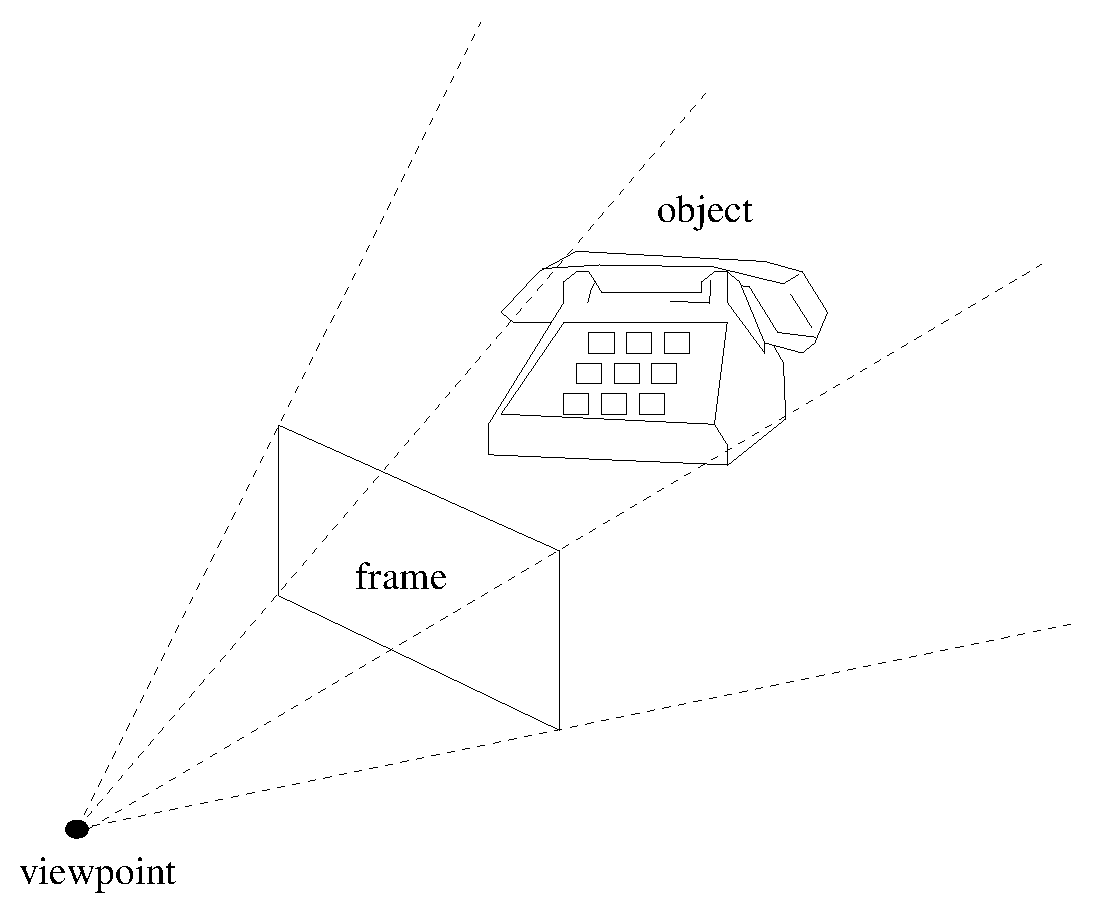
\includegraphics[width=2.3in, height=2in,angle = 0]{raytracing.ps}
\end{center}
\end{figure}
Lines ('rays') are extended from the viewpoint through a dense grid of points on the window,
and checked for intersection with the object.  If such an intersection exists, it should be 
registered as a point on the object 'visible' from the viewpoint.  In computer graphics, these 
points are projected back on the window, which becomes a 2D image that can be displayed on the
computer screen.  For our purposes, we refrain from doing this projection, and store the 
full 3D coordinates of the detected point.\\
Note that a ray may intersect the object more than once.  In these cases, the intersection point
closest to the viewpoint is chosen, as the other points are 'hidden' by it.  As mentioned above,
there are two raytracing routines in this example program.  The robust routine calculates all
possible intersection points for each ray, and then choses the nearest one.  This should always
work, but can be slow since no information is re-used.  When we have found an intersection point
for a given ray, we can usually expect that the next, neighouring ray will intersect in a point
close to the one already found.  If this is the case, it would be speedier to use a local 
algorithm that converges on the intersection point quickly given a good initial guess.  This is
the basis for our 'quick' routine.  This routine uses the robust raytracing algorithm to find
the first point on a surface, and then it switches over to the fast method as long as it is 
possible to do so.  However, since the quick method never finds more than one intersection point,
and since a ray may generally intersect an object more than once, we have no guarantee that
the point found is the one truly visible from the viewpoint.  There are some checking procedures
that make things better, but we still have no guarantee.   If the user inspects the results 
obtained, he will notice this problem even on the simple example given here.  In general, it
can be said that the rapid algorithm should only be used in some special cases, where we know
for a fact that any ray from the viewpoint will not intersect the surface more than once.\\

This is the only of the example programs that can be run with a command line argument.  If the 
first argument is \verb/q/, then the quick raytracing routine will be invoked.  Else, the
robust and slow routine is used.

\subsubsection{What it demonstrates}
\begin{enumerate}
\item The basic setting and principe of a raytracer, with a defined viewpoint, window and 
intersection with rays.
\item The use of the SISL routine \verb/s1856/, which calculates all intersections between a 
spline surface and a line.
\item The use of the SISL routine \verb/s1518/, which converges to an intersection between
a spline surface and a line, given a good initial guess.
\end{enumerate}
\subsubsection{Input/output}
The surface to be raytraced is read from the file \verb/example10_surf.g2/, generated by
the \verb/example10/ program.  The other parameters necessary for the raytracing are hard-
coded (viewpoint, view window, resolution, etc.).  The resulting points are written to the
file \verb/example15_points.g2/. 
\chapter{The object viewer program}

\section{General}
The object viewer program bundled with this distrubtion of SISL is intended to be
a simple but handy tool for visualising curves and surfaces generated by SISL.  The
supported file format is the \verb/Go/ (\textbf{G}eometric \textbf{O}bject) format, 
which is a simple, ASCII-based format defined by SINTEF.  The viewer is based on OpenGL. 
The object(s) to be viewed are specified on the command line when starting the 
program.  Once the program is started, the user cannot open other files containing
SISL objects.  The viewer allows the user to zoom, pan and rotate the objects with
the mouse, and some other useful commands can be accessed through the keyboard.
\\
\\
In the viewer window, several curves and surfaces can be displayed simultaneously.
At all times, exactly \emph{one} surface and \emph{one} curve are defined as being
\emph{active} (the other ones being \emph{passive}).  With keyboard commands, the user
can change the currently active surface/curve.  An object just becoming active will
flash for a few seconds.  With other keyboard commands, the user can \emph{enable/disable}
surfaces and curves.  This refers to turning the display of these objects on or off.
For details, refer to the section on keyboard commands.

\section{Command line arguments}
When starting up the viewer, the options listed below can be used.  If no option is
specified, a short text listing the available options is printed on screen.

\begin{itemize}
\item[$\bullet$] \textbf{\verb/s/} \textit{filename} - view the surface(s) contained in
the file \textit{filename}.  Note: this command line option can be used repetitively if
the user wants to inspect several surfaces at once.
\item[$\bullet$] \textbf{\verb/c/} \textit{filename} - view the curve(s) contained in the
file \textit{filename}.  Note: this command can be used repetitively if the user wants
to inspect several curves at once.
\item[$\bullet$] \textbf{\verb/p/} \textit{filename} - view the point(s) contained in 
the file \textit{filename}.  Note: this command line option can be used repetitively if
the user wants to inspect several surfaces at once.
\item[$\bullet$] \textbf{\verb/r/} \textit{integer} set surface refinement factor 
(number of facets in each direction on the surface). Default value is 100.  Higher values
gives smoother drawing of the surface.  NB: this option has to \emph{precede} the 's' 
option!
\item[$\bullet$] \textbf{\verb/e/} \textit{string} the string contains keypresses to execute
directly upon start (see the section on keyboard control keys for details).
\item[$\bullet$] \textbf{\verb/hotkeys/} does not start the viewer, but displays a list 
of keyboard commands that can be used when viewing.
\end{itemize}

A file can contain one or several curves, or one or several surfaces.  Files containing
both curves and surfaces are not supported.  The viewer can read several files to be
viewed at once.  On the command line, each ``curve'' file should be preceded with the
letter 'c', and each ``surface'' file should be preceded with the letter 's'.  After 
launch, all the objects contained in the given files are shown simultaneously.  The user
can disable the view of certain curves and surfaces if he or she wants to.  

\section{User controls}

After program launch, the viewing of curves and surfaces can be controlled with the mouse
and keyboard.  The mouse is used to define viewing angle, direction and zoom factor, while
keyboard keys are used to turn on/off objects and to change certain view parameters.

\subsection{Mouse commands}
It is assumed that a 3-button mouse is used.  By dragging the mouse while holding down the
\emph{left button}, the user can rotate the current view in an intuitive way.  By dragging
with a certain speed, the view will continue to rotate even after the left button is released.
The \emph{middle button} is used for zooming.  Hold down this button and move the mouse 
forwards and backwards in order to zoom in and out.  Holding down the \emph{right button}
while dragging the mouse moves the view up and down.

\subsection{Keyboard commands}

The available keyboard commands are:

\begin{itemize}
\item[$\bullet$] \textbf{\verb/q/} - quit the viewer program
\item[$\bullet$] \textbf{\verb/<space>/} - change the currently active curve 
(cycles through each of them)
\item[$\bullet$] \textbf{\verb/<tab>/} - change the currently active surface 
(cycles through each of them)
\item[$\bullet$] \textbf{\verb/w/} - turn on/off the wireframe display for surfaces
\item[$\bullet$] \textbf{\verb/B/} - toggle between black and white color for backgrounds
\item[$\bullet$] \textbf{\verb/A/} - toggle drawing of coordinate axes on/off
\item[$\bullet$] \textbf{\verb/S/} - toggle drawing of surfaces
\item[$\bullet$] \textbf{\verb/e/} - toggle visibility of currently active surface
\item[$\bullet$] \textbf{\verb/a/} - make all loaded surfaces visible
\item[$\bullet$] \textbf{\verb/d/} - hide all surfaces except the currently active one
\item[$\bullet$] \textbf{\verb/<ctrl>-e/} - toggle visibility of currently active curve
\item[$\bullet$] \textbf{\verb/<ctrl>-a/} - make all loaded curves visible
\item[$\bullet$] \textbf{\verb/<ctrl>-d/} - hide all curves except the currently active one
\item[$\bullet$] \textbf{\verb/O/} - center all objects around origo, and rescale objects
so that they fit inside the unit volume (does not preserve aspect ratio)
\item[$\bullet$] \textbf{\verb/o/} - center all objects around origo, no rescaling
\item[$\bullet$] \textbf{\verb/+/} - increase thickness of axes
\item[$\bullet$] \textbf{\verb/-/} - decrease thickness of axes
\item[$\bullet$] \textbf{\verb/>/} - increase size of points
\item[$\bullet$] \textbf{\verb/</} - decrease size of points
\item[$\bullet$] \textbf{\verb-/-} - decrease length of axes
\item[$\bullet$] \textbf{\verb/<esc>-w-[n]/} - store viewpoint in slot [n], where [n]
is a number from 0 to 9.  The viewpoint will be saved to file, and can such be preserved
from one session to another.
\item[$\bullet$] \textbf{\verb/<esc>-r-[n]/} - load a previously saved viewpoint from
slot [n], where [n] is a number from 0 to 9.
\end{itemize}

\cleardoublepage
\chapter{Appendix: Error Codes}
\label{errorcodes}
For reference, here is a list of the error codes used in SISL.
They can be useful for diagnosing problems encountered
when calling SISL routines.
However please note that a small number of SISL routines
use their own convention.

\begin{verbatim}
Label Value  Description
--------------------------------------------------------------------------------
err101 -101  Error in memory allocation.

err102 -102  Error in input. Dimension less than 1.

err103 -103  Error in input. Dimension less than 2.

err104 -104  Error in input. Dimension not equal 3.

err105 -105  Error in input. Dimension not equal 2 or 3.

err106 -106  Error in input. Conflicting dimensions.

err107 -107  			

err108 -108  Error in input. Dimension not equal 2.

err109 -109  Error in input. Order less than 2.

err110 -110  Error in Curve description. Order less than 1.

err111 -111  Error in Curve description. Number of vertices less than order.

err112 -112  Error in Curve description. Error in knot vector.

err113 -113  Error in Curve description. Unknown kind of Curve.

err114 -114  Error in Curve description. Open Curve when expecting closed.

err115 -115  Error in Surf description. Order less than 1.

err116 -116  Error in Surf description. Number of vertices less than order.

err117 -117  Error in Surf description. Error in knot vector.

err118 -118  Error in Surf description. Unknown kind of Surf.

err119 -119

err120 -120  Error in input. Negative relative tolerance.

err121 -121  Error in input. Unknown kind of Object.

err122 -122  Error in input. Unexpected kind of Object found.

err123 -123  Error in input. Parameter direction does not exist.

err124 -124  Error in input. Zero length parameter interval.

err125 -125

err126 -126

err127 -127  Error in input. The whole curve lies on axis.

err128 -128

err129 -129

err130 -130  Error in input. Parameter value is outside parameter area.

err131 -131

err132 -132

err133 -133

err134 -134

err135 -135  Error in data structure.
             Intersection point exists when it should not.

err136 -136  Error in data structure.
             Intersection list exists when it should not.

err137 -137  Error in data structure.
             Expected intersection point not found.

err138 -138  Error in data structure.
             Wrong number of intersections on edges/endpoints.

err139 -139  Error in data structure.
             Edge intersection does not lie on edge/endpoint.

err140 -140  Error in data structure. Intersection interval crosses
             subdivision line when not expected to.
   						
err141 -141  Error in input. Illegal edge point requested.

err142 -142  

err143 -143

err144 -144  Unknown kind of intersection curve.

err145 -145  Unknown kind of intersection list (internal format).

err146 -146  Unknown kind of intersection type.

err147 -147

err148 -147

err149 -149

err150 -150  Error in input. NULL pointer was given.

err151 -151  Error in input. One or more illegal input values.

err152 -152  Too many knots to insert.

err153 -153  Lower level routine reported error. SHOULD use label "error".

err154 -154

err155 -155

err156 -156  Illegal derivative requested. Change this label to err178.

err157 -157

err158 -158  Intersection point outside Curve.

err159 -159  No of vertices less than 1. SHOULD USE err111 or err116.

err160 -160  Error in dimension of interpolation problem.

err161 -161  Error in interpolation problem.

err162 -162  Matrix may be noninvertible.

err163 -163  Matrix part contains diagonal elements.

err164 -164  No point conditions specified in interpolation problem.

err165 -165  Error in interpolation problem.

err166 -166

err167 -167

err168 -168

err169 -169

err170 -170  Internal error: Error in moving knot values.

err171 -171  Memory allocation failure: Could not create curve or surface.

err172 -172  Input error, inarr < 1 || inarr > 3.

err173 -173  Direction vector zero length.

err174 -174  Degenerate condition.

err175 -175  Unknown degree/type of implicit surface.

err176 -176  Unexpected iteration situation.

err177 -177  Error in input. Negative step length requested.

err178 -178  Illegal derivative requested.

err179 -179  No. of Curves < 2.

err180 -180  Error in torus description.

err181 -181  Too few points as input.

err182 -182

err183 -183  Order(s) specified to low.

err184 -184  Negative tolerance given.

err185 -185  Only degenerate or singular guide points.

err186 -186  Special error in traversal of curves.

err187 -187  Error in description of input curves.

err188 -188

err189 -189

err190 -190  Too small array for storing Curve segments.

err191 -191  Error in inserted parameter number.

err192 -192

err193 -193

err194 -194

err195 -195

err196 -196

err197 -197

err198 -198

err199 -199  Error in vectors?
\end{verbatim}

\cleardoublepage
\input{licensing_information}
\cleardoublepage
\printindex
\end{document}
